\documentclass[11pt,oneside]{book}
\usepackage[T1]{fontenc}
\usepackage[utf8]{inputenc}
\usepackage{lmodern,microtype,amsmath,amssymb,amsthm,mathtools,mathrsfs}
\usepackage[margin=30mm,headheight=15pt]{geometry}
\usepackage{booktabs,longtable,array,enumitem,xcolor,graphicx}
\usepackage{tikz}
\usetikzlibrary{arrows.meta,positioning,calc,fit,decorations.pathreplacing,patterns,intersections}
\usepackage[unicode,colorlinks=true,linkcolor=blue!45!black,citecolor=green!35!black,urlcolor=blue!55!black]{hyperref}
\usepackage{xurl}
\usepackage{fancyhdr}
\pagestyle{fancy}\fancyhf{}\fancyhead[L]{\small\nouppercase{\leftmark}}\fancyhead[R]{\thepage}
\renewcommand{\chaptermark}[1]{\markboth{\thechapter.\ #1}{}}
\setlength{\emergencystretch}{3em}
\setlist{topsep=5pt,itemsep=3pt}
\numberwithin{equation}{chapter}
\newtheorem{theorem}{Theorem}[chapter]
\newtheorem{lemma}[theorem]{Lemma}
\newtheorem{proposition}[theorem]{Proposition}
\newtheorem{corollary}[theorem]{Corollary}
\theoremstyle{definition}\newtheorem{definition}[theorem]{Definition}
\newtheorem{example}[theorem]{Example}
\theoremstyle{remark}\newtheorem{remark}[theorem]{Remark}
\newcommand{\ii}{\mathrm i}
\newcommand{\dd}{\mathrm d}
\newcommand{\CC}{\mathbb C}
\newcommand{\RR}{\mathbb R}
\newcommand{\ZZ}{\mathbb Z}
\newcommand{\NN}{\mathbb N}
\newcommand{\cH}{\mathcal H}
\newcommand{\cA}{\mathcal A}
\newcommand{\cP}{\mathcal P}
\newcommand{\cD}{\mathcal D}
\newcommand{\Bhat}{\widehat B}
\newcommand{\Turn}{\mathsf T}
\newcommand{\Cheb}{\mathsf C}
\newcommand{\Closure}{\mathsf C\!\ell}
\newcommand{\Vol}{\operatorname{Vol}}
\newcommand{\Tr}{\operatorname{Tr}}
\newcommand{\Res}{\operatorname{Res}}
\newcommand{\supp}{\operatorname{supp}}
\newcommand{\arccot}{\operatorname{arccot}}
\newcommand{\dist}{\operatorname{dist}}
\newcommand{\diag}{\operatorname{diag}}
\newcommand{\co}{\operatorname{co}}
\newcommand{\poly}{\operatorname{poly}}
\newcommand{\eps}{\varepsilon}
\newcommand{\sourcefile}[1]{\texttt{\detokenize{#1}}}
\tikzset{box/.style={draw,rounded corners,fill=blue!4,align=center,inner sep=7pt}, arr/.style={-{Latex[length=2mm]},thick}, port/.style={draw,fill=white,minimum size=4mm,circle,inner sep=0pt}}
\title{\Huge Volume limits for arborescent knots\\[8pt]\Large Long twists and explicit conditions\\for ordered tangle trees\\[18pt]\large Finite knot invariants, hyperbolic filling,\\and the preferred cusp shape}
\author{}
\date{1 November 2026}
\begin{document}
\hypersetup{pageanchor=false}
\maketitle
\clearpage
\hypersetup{pageanchor=true}
\frontmatter
\chapter*{Abstract}
We prove the volume conjecture for two specified classes of arborescent knot diagrams built by ordered stacking and quarter-turns of two-string tangles. The first is a recursive construction in which independently sufficiently large signed twist numbers give a hyperbolic knot and the volume limit. Its elementary pieces retain their original crossing circles, disk framings and endpoint order.

For ordered trees with one crossing-circle operator at every vertex, we give explicit sufficient conditions in the vertex degree $d_v$ and signed crossing power $n_v$. One condition is
\[
                  \sum_v\frac{d_v}{d_v^2+n_v^2}\le2^{-25}.
\]
A separate local argument proves the volume identity whenever, at every vertex,
\[
                   d_v\ge2^{28}\qquad\hbox{or}\qquad |n_v|\ge2^{27}.
\]
Thus $|n_v|\ge2^{27}$ suffices independently of the number of tangles. The degree alternative also permits any fixed short or zero powers at sufficiently large-degree vertices. A more flexible finite criterion allows a separate decay constant on each attaching edge and distinguishes the final vertex of the calculation. Every diagram and all its integer powers are fixed before the root-of-unity level $N$ tends to infinity. The original strand connections must give one knot, with no internally closed extra component.

The proof begins with the finite matrices defining the invariant and retains their derivative data at repeated spectral roots. For the long-twist construction, positive multiplication coefficients and exact rational inequalities control the signed color terms. For the quantitative tree theorems, a cut of the actual augmented exterior gives two octahedra per edge. Their positive deformations and primitive peripheral periods construct the metric after filling. The quantum calculation evaluates subtrees as exact polynomials, keeps their values at zero, and bounds every Fourier contribution relative to the next conditional critical value. This proves noncancellation and identifies the limiting action with the volume of the original knot complement. Only auxiliary circles are filled; the main knot cusp remains complete.

The same calculation gives a uniform microscopic main-meridian profile for the zero-framed reduced ADO invariant. The exact crossing and framing factors remain in the formula. The summed theorem also identifies the first correction with the preferred cusp shape. By attaching even stacks of sufficiently long terminal tangles to any fixed knot-paired circle-tree core, the degree alternative produces examples retaining arbitrarily many prescribed short-twist pieces. These attachments preserve the endpoint pairing and can change the knot.

Finally, the full asymptotic source determines the preferred geometric longitude on the previously covered strict Conway branches, including product junctions without crossing circles. The proof first treats circle trees by explicit representations and algebraic rigidity. At an unmarked junction, inserting a zero-crossing box and an auxiliary circle preserves the original tangle after meridian filling; an exact stationary elimination and the based boundary maps extend the longitude identity. It follows that the selected geometric irreducible factor divides the first nonzero classical symbol of every genuine all-level annihilator under the stated full-source hypotheses. This is a statement about the selected factor, not the entire A-polynomial or recurrence ideal.

\tableofcontents
\mainmatter
\chapter{The theorem and its scope}\label{ch:introduction}

\section{The problem}
The volume conjecture compares two objects with very different definitions: a finite root-of-unity knot invariant and the complete hyperbolic metric of a knot complement. Kashaev's finite invariant was introduced in \cite{Kashaev1995}; the asymptotic volume proposal appeared in \cite{Kashaev1997}. The relation with the root-of-unity specialization of the colored Jones polynomial is part of the historical setting \cite{MurakamiMurakami2001}. Here the invariant is fixed by explicit matrices and a specified enhancement. The comparison with that conventional normalization is proved by finite identities, rather than used to replace the source by another state integral.

A long-twist theorem has two limits that must be separated. First choose a diagram and a tuple of sufficiently large integer twists. These integers are then held fixed while the level $N$ tends to infinity. The proof must therefore control the whole finite invariant at every large level, not just a favorable color, a positive coefficient, or a formal solution of a recurrence. In particular, the oscillations responsible for the smaller volume after filling cannot be removed by taking absolute values before the filling transform.

This manuscript treats a compositional family. The local objects have four ordered boundary points, so products and turns can be compiled without choosing a new global decomposition at each stage. The main difficulty is that the exact mixed-color leaf contains a second, signed part, called its \emph{alias}. The compositional estimate controls that part when one leaf is attached to a completed child. It is a global supporting-plane inequality on the actual multiplication domain. Its proof uses a finite collection of rational inequalities with rigorous transcendental enclosures.

\section{Ordered tangles and completed expressions}
An elementary augmented tangle consists of two main strands encircled by one auxiliary crossing circle. Write $L$ for that four-port box and $h=\Turn L$ for its ordered quarter-turn. Product means the literal vertical stack, with the two intermediate strands joined in their recorded order. A turn bends the original boundary strands using the original cup and cap. Neither operation permits an unrecorded permutation of ports.

\begin{definition}[Completed grammar]\label{def:grammar}
A completed expression is generated by
\begin{equation}\label{eq:grammar}
 E ::= hh\ \mid\ \Turn(E)\ \mid\ E_1E_2\ \mid\ hE\ \mid\ Eh.
\end{equation}
Every occurrence of $h$ denotes a distinct crossing circle and an independent auxiliary color. A closed expression in the main theorem is the cylindrical closure $C(FG)$, where both $F$ and $G$ are completed. Its ribbon framing, local disk framings and one global cut are retained throughout.
\end{definition}

The equivalent convention allowing every $h^s$, $s\ge2$, as an initial block gives the same grammar. Arbitrary finite nesting and repeated chains such as $E_{n+1}=h\Turn(E_n)$, $E_0=hh$, are allowed. The restriction on the two root children is substantive: strict feasibility alone does not give the selected high-index complex packet needed below.

At leaf $\ell$, choose $\eps_\ell\in\{0,1,-1\}$ and retain the corresponding physical half twist. Filling the crossing circle by the original disk-framed power $R^{-2p_\ell}$ replaces that leaf by the actual rational tangle
\begin{equation}\label{eq:rational-leaf}
 \Turn\bigl(R^{\eps_\ell-2p_\ell}\bigr).
\end{equation}
Choose the signs so that the endpoint pairing gives one main component and no closed component inside the tangle tree. An elementary pairing induction, proved in Section~\ref{sec:pairings}, supplies such a choice. After every auxiliary filling, no crossing-circle component remains. Products and quarter-turns of the rational tangles in \eqref{eq:rational-leaf} give a Conway algebraic link; with the chosen pairing it is a knot. This is a membership statement derived from actual tangle operations. Equality of source scalars will never be used as a substitute for tangle isotopy.

\begin{theorem}[Long-twist volume limit]\label{thm:main}
Fix a finite expression $C(FG)$ as in Definition~\ref{def:grammar} and a half-twist pattern $\eps$ giving a knot. There is a finite number $P(F,G,\eps)$ such that, for every independently chosen tuple of signed integers $\mathbf p=(p_\ell)$ with $|p_\ell|>P(F,G,\eps)$, the resulting knot $K_{F,G,\eps}(\mathbf p)$ is hyperbolic and
\begin{equation}\label{eq:main-volume}
 \lim_{N\to\infty}\frac{2\pi}{N}
 \log\left|\langle K_{F,G,\eps}(\mathbf p)\rangle_N\right|
 =\Vol\bigl(S^3\setminus K_{F,G,\eps}(\mathbf p)\bigr).
\end{equation}
The level tends to infinity through all integers, including even and composite levels. The expression, signs and twists are fixed before that limit. The threshold depends on the fixed expression and sign pattern, but not on a comparison between the magnitudes or signs of the individual sufficiently long twists.
\end{theorem}

The notation $\langle\cdot\rangle_N$ denotes the enhanced reduced invariant with unknot value one specified in Chapter~\ref{ch:source}. The full modified one-cut normalization differs by the single factor $\ii^{N+3}/N$ and a unit framing character, and therefore has the same limit. There is only one such modified factor, on the marked main component. The auxiliary circles use ordinary pivotal traces.

The already established isolated closures $C(h^s)$, $s\ge3$, can be included as a separate inherited family. The case $C(h^3)$ is described explicitly in Section~\ref{sec:isolated}. The isolated $C(hh)$ is excluded: its even-level source is zero, and its odd-level source is confined to a flat boundary. More general root-leaf closures $C(hE)$ are not included in Theorem~\ref{thm:main}. For example, in $C(h\Turn(h^s))$ the inner complete leaf indices equal $1/4$, at the boundary of the uniform packet used here.

\section{Proof architecture}
There are four logically distinct comparisons. First, finite matrix identities express the original scalar in a nonsemisimple polynomial algebra. Second, the complete positive source has a strict entropy maximizer, and explicit ideal cells identify its action with the volume of the actual augmented-link complement. Third, rigorous alias bounds and a finite complex lattice saddle produce a nonzero packet for the original mixed source. Finally, the exact filling transform selects a nonzero charge contribution whose critical action is the volume after filling.

\begin{figure}[ht]
\centering
\begin{tikzpicture}[node distance=8mm, every node/.style={font=\small}]
\node[box,text width=11.5cm] (s) {Evaluate the augmented tangle by its finite matrices\\Keep both polynomial values and derivatives at repeated roots};
\node[box,below=of s,text width=11.5cm] (p) {Maximize the positive complete-color sum\\Build its ideal cells and recover the actual augmented link metric};
\node[box,below=of p,text width=11.5cm] (a) {Bound the signed complementary color terms throughout the construction\\Obtain a nonzero holomorphic asymptotic near the complete maximum};
\node[box,below=of a,text width=11.5cm] (f) {Evaluate the entire oscillatory filling sum\\Keep contour boundary terms and identify the primitive filling slope};
\node[box,below=of f,text width=11.5cm,fill=green!5] (v) {The actual knot complement after all auxiliary fillings\\$N^{-1}\log|\langle K\rangle_N|\longrightarrow\Vol(S^3\setminus K)/(2\pi)$};
\draw[arr] (s)--(p);\draw[arr] (p)--(a);\draw[arr] (a)--(f);\draw[arr] (f)--(v);
\end{tikzpicture}

\caption{The proof keeps the finite source and the geometric marking together. A complete-color volume identity alone would not justify the final arrow.}\label{fig:architecture}
\end{figure}

Each comparison has an obstruction that explains its formulation. Repeated Casimir roots prevent a replacement by values at distinct nodes. The complete circle is nilpotent at even levels, so a fixed complete-color operator cannot be inverted to perform filling. Positive coefficients control the complete action but not the signed aliases. An asymptotic expansion at a single real color does not control a complex saddle displaced by a fixed long filling. Finally, the full filling period has both endpoint currents and infinitely many Fourier charges. The proof retains these features instead of hiding them in a normalization or a formal stationary-phase argument.

\section{Conventions and proof records}
All logarithms on a positive real interval are real. Their complex continuations are selected from that interval and are used only on explicitly chosen zero-free neighborhoods. Put $\arccot X\in(0,\pi)$ for real $X$, and write $\ii^2=-1$. A constant may depend on the fixed tangle tree, its chosen strict stationary point and a fixed compact analytic neighborhood, but never on $N$. A polynomial factor means $N^C$ for such a fixed constant $C$.

The appendices give the finite identities and the analytic estimates used in the main proof. The exact rational certificates are finite mathematical objects, rather than fitted numerical data: their verifier checks coverage, supporting inequalities and every outward-rounding remainder. Chapter~\ref{ch:reproduction} separates these checks from the continuum arguments. Internal proof review and successful execution are reported as such; neither is described as external peer review.

\chapter{Evaluating the invariant in a finite polynomial algebra}\label{ch:source}

We now turn the tangle operations of Chapter~\ref{ch:introduction} into finite matrix calculations. A strand carries a finite-dimensional vector space, a crossing acts on the two corresponding factors, and joining endpoints means contracting the appropriate indices. Closing an auxiliary circle takes a trace. Leaving one marked main strand open until the final contraction gives the reduced normalization.

The purpose of the polynomial algebra introduced below is to make these contractions compositional. Every two-strand operator that occurs here is a polynomial in one matrix, the pair Casimir $\Omega$. Stacking becomes multiplication of polynomials, while the quarter-turn has a particularly simple action in the Newton basis. The last section then expresses an arbitrary filling power in the basis of colored auxiliary-circle operators. All of these statements are finite identities at each level; asymptotics begin only in Chapter~\ref{ch:entropy}.

\section{Crossings and the one-cut normalization}
Fix $N\ge2$, and set
\begin{equation}\label{eq:root-notation}
 d=N-1,\qquad q=e^{\pi\ii/N},\qquad Q=q^2,\qquad
 x=q^d,\qquad \kappa=q^{d^2/2},\qquad \rho=q-q^{-1}.
\end{equation}
There is no restriction to prime or odd $N$. The main strands carry the $N$-dimensional vector space $V_N$; this is what ``complete color'' means at this stage. The operators $H,K,E,F$ encode its quantum-group action. They are concrete matrices, which we specify so that the crossing convention can be checked. One convenient choice of basis is $v_0,\ldots,v_d$ and
\[
 H v_j=(d-2j)v_j,\quad K=q^H,\quad
 E v_j=[j]_q^2v_{j-1},\quad Fv_j=v_{j+1},
 \qquad [j]_q=\frac{q^j-q^{-j}}{q-q^{-1}}.
\]
Missing endpoint vectors are zero. For $k\ge0$, the quantum factorial is
$[k]_q!=\prod_{r=1}^k[r]_q$, with $[0]_q!=1$.
The finite universal crossing, including its Cartan factor, is
\begin{equation}\label{eq:universal-crossing}
 \mathscr R=q^{H\otimes H/2}
 \sum_{k=0}^{d}\frac{q^{k(k-1)/2}\rho^k}{[k]_q!}
 E^k\otimes F^k.
\end{equation}
Every denominator is nonzero. The physical braided crossing is obtained with the fixed exchange and transpose convention; the inverse is the actual matrix inverse. The framing and enhancement are part of the definition, not an unspecified factor appended to an asymptotic formula.

For calculations in the polynomial algebra it is useful to change basis on this same space. We call the new coordinates balanced; they do not define a different invariant. In this basis the operators are
\begin{equation}\label{eq:balanced-module}
 \mathcal E|a\rangle=(Q^{-a}-1)|a-1\rangle,\quad
 \mathcal F|a\rangle=(1-Q^{a+1})|a+1\rangle,\quad
 K|a\rangle=xQ^{-a}|a\rangle.
\end{equation}
The ordinary cup and cap, and the one marked cap, have entries
\begin{equation}\label{eq:cups}
 p_{ab}=Nx^{-b}\delta_{a+b,d},\qquad
 \ell_{ab}=\frac{x^a}{N}\delta_{a+b,d},\qquad
 m_{ab}=\frac{x^b}{N^2}.
\end{equation}
The cup creates two endpoints and the cap joins them. Their two snake identities say that a bend followed by the opposite bend evaluates to a straight strand. The different marked cap implements the reduced invariant and satisfies $mp=1$. The diagonal operator $g=K^{1-N}=(-1)^dK$ is the \emph{pivot}, the correction inserted when an ordinary strand is closed by a trace. For a two-strand operator $A$ commuting with the pair quantum-group action, the original cylindrical evaluation is
\begin{equation}\label{eq:phi-physical}
 \phi(A)=\frac1N\Tr_{V_N\otimes V_N}\bigl[(I\otimes g)A\bigr].
\end{equation}
The factor $1/N$ in this expression is the single cut average. It is not repeated at the auxiliary circles.

\begin{proposition}[Normalization]\label{prop:normalization}
Let $A_{\rm raw}$ be the scalar obtained from the original crossings, turns, ordinary auxiliary traces and the single mark. In the enhanced reduced Kashaev convention,
\[
 |\langle L\rangle_N|=|A_{\rm raw}(L)|.
\]
In the full modified one-cut convention the modulus is $N^{-1}|A_{\rm raw}(L)|$. The changes of recorded component framing contribute only unit phases at the complete color.
\end{proposition}
\begin{proof}
The exact Fourier comparison is recorded in Appendix~\ref{app:normalization}. It is a simultaneous similarity of every adjacent braid generator and its inverse, together with an exact equality of enhancements. The factorial changes of basis cancel on every internal or traced wire. On the one remaining head the partial trace is scalar: it commutes with $E,F,K$, whose distinct weights and nonzero adjacent coefficients force scalarity. Hence the open-factor similarity cancels as well.

For clarity, the complete modified dimension is evaluated as a whole meridian germ. With the original meridian $M=-q q^\alpha=e^u$,
\[
 d_N(\alpha)=-q^{N(1-N)/2}
 \frac{q^{\alpha+1}-q^{-\alpha-1}}{q^{N\alpha}-q^{-N\alpha}}
 =\ii^{N+3}\frac{\sinh u}{\sinh Nu}.
\]
Its removable value at $u=0$ is $\ii^{N+3}/N$. Exactly one component receives this factor. The twist at completeness is $q^{-d^2/2}=\kappa^{-1}$, of modulus one. These facts prove the asserted absolute normalization without estimating any large change-of-basis matrix.
\end{proof}

\section{The full pair algebra}

An operator on two strands must commute with the joint action of the quantum-group generators if it is to represent one of our invariant tangle boxes. The formulas below specify that joint action. The subsequent lemma identifies all such commuting operators; this is the meaning of the term \emph{commutant}.
The balanced pair generators and Casimir are
\begin{equation}\label{eq:pair-casimir}
 \mathcal E_{12}=\mathcal E_1K_2+\mathcal E_2,\quad
 \mathcal F_{12}=\mathcal F_1+K_1^{-1}\mathcal F_2,\quad
 K_{12}=K_1K_2,\quad
 \Omega=\mathcal F_{12}\mathcal E_{12}+qK_{12}+q^{-1}K_{12}^{-1}.
\end{equation}
Let $\Cheb_n(z)=2T_n(z/2)$, where $T_n$ is the usual Chebyshev polynomial. Thus $\Cheb_0=2$, $\Cheb_1=z$ and $\Cheb_{n+1}=z\Cheb_n-\Cheb_{n-1}$. Define
\begin{equation}\label{eq:hermite-algebra}
 P_N(z)=\Cheb_N(z)+2=\prod_{j=0}^{d}(z-c_j),\qquad
 c_j=q^{2j+1}+q^{-2j-1},\qquad
 \cH_N=\CC[z]/(P_N).
\end{equation}
The list of roots includes multiplicity. Since $c_{d-j}=c_j$, all distinct roots are double except the simple root $-2$ at odd $N$.

\begin{lemma}[Full commutant]\label{lem:commutant}
The endomorphisms of $V_N\otimes V_N$ commuting with the three pair generators are exactly $\CC[\Omega]\simeq\cH_N$.
\end{lemma}
\begin{proof}
Let $W_T$ be the span of $|a,T-a\rangle$. The $K_{12}$ eigenvalue one occurs only on $W_d$. The matrices $\mathcal E_{12}:W_{T+1}\to W_T$ for $T<d$, and $\mathcal F_{12}:W_T\to W_{T+1}$ for $T\ge d$, have triangular maximal minors with nonzero diagonals. Consequently the entire pair is generated from $W_d$ by these raising and lowering operators.

On $W_d$, the Casimir is a symmetric tridiagonal matrix with adjacent entries $-(1-Q^{a+1})^2\ne0$. Its first basis vector is cyclic: the $k$th power has last possible coordinate $k$, with coefficient equal to the nonzero product of the first $k$ adjacent entries. An operator commuting with this block is therefore a unique polynomial of degree below $N$ in that block. Subtracting the same polynomial in $\Omega$ from a pair intertwiner gives zero on $W_d$, hence zero everywhere by generation.

The elementary quantum-shift product gives $P_N(\Omega)=0$. The cyclic block has minimal polynomial of degree $N$; its continuant, or the generic highest-weight decomposition followed by regular specialization, gives precisely \eqref{eq:hermite-algebra}. This proves the claim with all first normal directions intact.
\end{proof}

At a double root $c$, reduction modulo $(z-c)^2$ leaves
\[
 f(z)=f(c)+f'(c)(z-c)\pmod{(z-c)^2}.
\]
Thus both the value and its first derivative are independent coordinates of the operator. Throughout the paper, retaining the ``full algebra'' or the ``normal data'' means retaining this derivative as well. A polynomial can vanish at every distinct root and still define a nonzero operator in $\cH_N$. Evaluating only at roots would therefore lose part of the invariant.

\section{The actual turn and the Newton basis}

We choose a polynomial basis adapted to successive Casimir roots, including their multiplicities. Its normalization is designed so that turning a physical box reverses the basis index exactly. The same basis makes the final closure a coefficient extraction. These are the two facts that will allow us to follow every internal summation index through a large construction.
Put
\begin{equation}\label{eq:newton-basis}
 s_r=\prod_{u=1}^{r}2\sin\frac{\pi u}{N},\quad s_0=1,\qquad
 B_r(z)=\prod_{j=0}^{r-1}(c_j-z),\qquad
 \Bhat_r(z)=\frac{B_r(z)}{s_r^2},\quad 0\le r\le d.
\end{equation}
The quarter-turn is the literal contraction
\[
 \Turn(A)=(I^{\otimes2}\otimes\ell)(I\otimes A\otimes I)
 (p\otimes I^{\otimes2}).
\]
Its entries in the recorded all-primal chart are
\[
 \Turn(A)_{(a,b);(c,e)}=x^{a-e}A_{(b,d-e);(d-a,c)}.
\]
The cups and caps are those of \eqref{eq:cups}. A different source-normalized rotation can carry an additional power of $x$; throughout this manuscript $\Turn$ is the unscaled genuine turn.

\begin{proposition}[Newton turn and closure]\label{prop:newton-turn}
In the full algebra,
\begin{equation}\label{eq:newton-turn}
 \Turn\Bhat_r=\Bhat_{d-r},\qquad
 \phi\left(\sum_{r=0}^{d}\alpha_r\Bhat_r\right)=\alpha_d,
 \qquad
 \phi(\Bhat_i\Bhat_j)=\delta_{i+j,d}.
\end{equation}
\end{proposition}
The finite verification is given in Appendix~\ref{app:newton}. It uses the physical turn, its nonzero adjacent charge-block entries and the finite quantum-binomial recurrence. In particular, \eqref{eq:newton-turn} is not a generic-$q$ continuation of a formula checked only on distinct root values. The turn is linear and involutive in this basis, but is not multiplicative.

The same closure can be displayed directly in Hermite coordinates:
\begin{equation}\label{eq:hermite-trace}
 \phi(f)=(-1)^d\sum_{c\ {
m double}}
 \bigl((4-c^2)f'(c)-cf(c)\bigr)
 +\mathbf1_{N\ {
m odd}}f(-2).
\end{equation}
Equivalently,
\begin{equation}\label{eq:leading-trace}
 \phi(f)=(-1)^dN^2[z^d](f\bmod P_N).
\end{equation}
For example, at a double root $c$, writing $Q_c=P_N/(z-c)^2$ gives
$Q_c(c)=N^2/(4-c^2)$ and $Q_c'(c)/Q_c(c)=c/(4-c^2)$ from the Chebyshev differential equation. The residue of $f/P_N$ is exactly the corresponding term of \eqref{eq:hermite-trace} after multiplication by $(-1)^dN^2$. Summing residues proves \eqref{eq:leading-trace}; the simple odd root has $P_N'(-2)=N^2$. The sole shortest tridiagonal path from the first to the last coordinate has product $(-1)^dN^2$, which also identifies this scalar with the original endpoint matrix element.

\section{Positive multiplication with every normal retained}

Suppose two stacked boxes contribute basis indices $i$ and $j$. Their product is a linear combination of output indices $r$. The following coefficient formula gives both the allowed triples $(i,j,r)$ and their weights. Calling this local operation a \emph{gate} is only shorthand for this one multiplication; the geometric operation remains the vertical stack.
\begin{theorem}[Multiplication law]\label{thm:positive-product}
If $i+j<N$, then
\begin{equation}\label{eq:positive-product}
 \Bhat_i\Bhat_j=\sum_{r=\max(i,j)}^{i+j}\mu_{ijr}\Bhat_r,
 \qquad
 \mu_{ijr}=\frac{s_{i+j}s_r}
 {s_i s_j s_{r-i}s_{r-j}s_{i+j-r}}>0.
\end{equation}
If $i+j\ge N$, the product is zero in the full algebra. In particular, a product gate has precisely the integer support
\begin{equation}\label{eq:gate-support}
 i+j\le d,\qquad \max(i,j)\le r\le i+j.
\end{equation}
\end{theorem}
\begin{proof}
At a generic parameter $\zeta$, put $t=-(\zeta-\zeta^{-1})^2$. The unnormalized coefficients are
\[
 B_iB_j=\sum_r
 t^{i+j-r}\frac{[i]![j]![i+j]!}
 {[r]![r-i]![r-j]![i+j-r]!}\,B_r.
\]
Multiplication by $c_i-z$ and the identity
$(c_i-z)B_r=B_{r+1}+(c_i-c_r)B_r$, with
$c_i-c_r=t[r+i+1][r-i]$, reduce induction to
\[
 [i+1][i+j+1]=[r][r-j]+[r+i+1][i+j+1-r].
\]
This follows by expanding the four powers of $\zeta$. Endpoint coefficients follow from the same zero factors. At the principal root, all factorial indices in the case $i+j<N$ are below $N$. Since $[u]!=s_u/(2\sin(\pi/N))^u$, normalization by $s_i^2s_j^2/s_r^2$ gives \eqref{eq:positive-product}.

For $i+j\ge N$, use the exact polynomial identity $B_N/B_j=B_{N-j}$, a consequence of $c_{d-u}=c_u$. Then $B_iB_j$ is divisible by $B_N=(-1)^NP_N$ with multiplicities. This proves the zero assertion without dropping the first normal directions.
\end{proof}

\section{The literal crossing circle and its colors}

A color $j$ on an auxiliary circle means that the circle carries a $j$-dimensional representation. The main strands still carry $V_N$. We must compute the resulting operator on those two main strands, including the trace around the auxiliary circle, before replacing that circle by twists. The answer is a Chebyshev polynomial in $\Omega$, with the sign fixed by the pivot.
For $1\le j\le N$, the auxiliary module is the ordinary $j$-dimensional highest-weight module. Its loop is the actual block-braiding word $[2,1,1,2]$, with the intermediate strand dimensions retained, followed by its ordinary pivot $K_j^{1-N}$. There is no auxiliary $1/j$ or $1/N$.

\begin{proposition}[Circle identity]\label{prop:circle}
The resulting two-head operator is
\begin{equation}\label{eq:circle}
 L_j=(-1)^{j-1}U_{j-1}(\Omega/2).
\end{equation}
Here $U_0=1$, $U_1(z/2)=z$, and $U_{n+1}(z/2)=zU_n(z/2)-U_{n-1}(z/2)$.
\end{proposition}
\begin{proof}
At generic $q$, evaluate the closed monodromy on a target highest vector of weight $n$. In one direction the positive raising terms annihilate that vector; in the return direction a positive lowering term cannot return to its highest coefficient. The two Cartan factors and the auxiliary pivot give
\[
 \sum_{a=0}^{j-1}q^{(n+1)(j-1-2a)}
 =U_{j-1}\bigl((q^{n+1}+q^{-n-1})/2\bigr).
\]
The generic pair highest vectors have distinct Casimirs and descendants of total dimension $N^2$, so this proves the full matrix identity. All finite crossing denominators have indices below $N$, and the identity specializes regularly. Finally $K_j^{1-N}=(-1)^{j-1}K_j$ at the root, proving \eqref{eq:circle}, including its nilpotent coefficients.
\end{proof}

In particular $L_N=(-1)^dP_N'(\Omega)/N$. The trace identity
\begin{equation}\label{eq:circle-trace}
 \phi(L_Nf)=N\sum_{j=0}^{d}f(c_j)
\end{equation}
counts the repeated roots. It follows first by Lagrange interpolation for a polynomial with distinct roots and then by polynomial continuation in its coefficients. At even levels $L_N^2=0$; at odd levels $L_N^2=N^2E_{-2}$, with the simple-node projector $E_{-2}$. Thus complete color alone cannot be inverted to reconstruct a filling.

Let $M=\lfloor d/2\rfloor$ and $h_j=\Turn L_j$. The complete leaf has the exact positive expansion
\begin{equation}\label{eq:complete-leaf}
 h_N=\sum_{v=0}^{M}a_{N,v}\Bhat_v,
 \qquad a_{N,v}=\frac{N^2s_{2v}}{s_v^4}>0.
\end{equation}
For $0\le h\le M$, with $h_0=0$, the full color decomposition is
\begin{equation}\label{eq:core-alias}
 h_{N-h}=\sum_{v=h}^{M}
 \frac{N^2s_{2v}}{s_v^2s_{v-h}s_{v+h}}\Bhat_v+(-1)^Nh_h.
\end{equation}
For $1\le h\le\lfloor N/2\rfloor$,
\begin{equation}\label{eq:low-alias}
 h_h=\sum_{r=0}^{h-1}(-1)^{h-1+r}
 \frac{s_r^2s_{h+r}}{s_{2r+1}s_{h-r-1}}\Bhat_{d-r}.
\end{equation}
These identities separate two different ranges of Newton indices. The first term in \eqref{eq:core-alias}, called the \emph{core}, has positive coefficients before a half twist and occupies the lower indices. The second term, called the \emph{alias}, is an exact signed contribution from the complementary color; formula~\eqref{eq:low-alias} puts it in the higher Newton indices. An alias is therefore part of the finite invariant, not an error introduced by approximation. Appendix~\ref{app:colors} derives both formulas from the finite Chebyshev generating function. Chapter~\ref{ch:alias} will prove when the contribution of aliases is exponentially smaller after the complete tangle is assembled.

\section{Half twists and exact filling}

The preceding formulas describe a circle with no retained crossing. We next insert one positive or negative crossing in its original disk framing. This changes both the coefficients and their phases. We then expand a full integer twist power in the circle basis. Keeping these two steps separate ensures that the physical power is exactly $R^{\eps-2p}$, with the retained half twist counted once.
A retained half twist acts on a turned leaf by
$\Turn_\eps(f)=\Turn(R^\eps\Turn f)$, for $\eps=\pm1$. Its exact transport is
\begin{equation}\label{eq:half-twist}
 \Turn_\eps\Bhat_v=\kappa^\eps(-1)^v
 \sum_{r=0}^{v}q^{\eps v(r+1)}
 \frac{s_v}{s_rs_{v-r}}\Bhat_r.
\end{equation}
The triangular formula retains the full Cartan phase and all normals. Its derivation uses the finite continuant expansion and root factorial reflection; the two signs are coefficient conjugates in the real Newton basis. A half-twisted alias may occupy every Newton coordinate, so the pure alias support cannot be reused after \eqref{eq:half-twist}.

The $N$ circle polynomials $L_1,\ldots,L_N$ form a basis of $\cH_N$. The full crossing has a Hermite polynomial $R=\kappa r_N(\Omega)$ with
\[
 r_N(c_k)=(-1)^kq^{k(k+1)},\qquad
 \frac{r_N'(c_k)}{r_N(c_k)}
 =-\frac{d-2k}{2(q^{2k+1}-q^{-2k-1})}
\]
at each double node, and the stated value at the odd simple node. Fourier--Hermite interpolation therefore gives, for every integer $p$,
\begin{equation}\label{eq:exact-filling}
 R^{-2p}=\kappa^{-2p}\sum_{j=1}^{N}\beta_{j-1}^{-p}L_j,
 \qquad \sum_{j=1}^{N}|\beta_{j-1}^{-p}|\le2N(1+|p|).
\end{equation}
The notation $\beta_{j-1}^{-p}$ denotes the full interpolation coefficient, not a power of a scalar eigenvalue. Its value and derivative data are specified in Appendix~\ref{app:fourier}.

Insert \eqref{eq:exact-filling} at every original auxiliary disk, tensoring with the spectators before taking the unchanged closure. If $\mathcal A_N(\mathbf h)$ is the actual mixed source with colors $N-h_\ell$, then
\begin{equation}\label{eq:whole-filling-source}
 \langle K(\mathbf p)\rangle_N
 =\chi_N\kappa^{-2\sum p_\ell}
 \sum_{j_1,\ldots,j_H=1}^{N}
 \left(\prod_\ell\beta_{j_\ell-1}^{-p_\ell}\right)
 \mathcal A_N(N-j_1,\ldots,N-j_H).
\end{equation}
Here $|\chi_N|=1$ in the reduced convention. This is an all-input finite identity. The remainder of the proof analyzes this complete sum, rather than replacing it by the complete-color term.

\chapter{From the finite sum to an angle maximization problem}\label{ch:entropy}

At complete auxiliary color, every elementary coefficient and every multiplication coefficient is positive. We can therefore determine its exponential growth by maximizing the growth rate of an individual summand. This chapter makes that statement precise in three steps: determine the exact allowed integer indices, pass to their scaled compact polytope, and prove that the resulting action has a unique maximum away from every nonforced boundary. The same functions will then be recognized as hyperbolic volumes.

The distinction between an exact integer constraint and its limiting inequality matters here. We use $d=N-1$ in every finite relation. The replacement by a continuous variable is made only after those relations have been solved, so no parity condition or half-lattice factor is lost.

\section{Following the allowed indices through the construction}
Expand an expression into its individual leaves, turns and binary products. A leaf has the positive support $[0,M]\cap\ZZ$. A turn replaces an index $r$ by $d-r$. A product is governed by \eqref{eq:gate-support}. Thus the source is a finite sum over a fixed tree of integer labels, with a positive coefficient at every admissible state in the complete pure case. The closure selects output $d$.

The finite support can be computed without evaluating any transcendental number. If a positive expression has interval support $[l,u]\cap\ZZ$, its turn has support $[d-u,d-l]\cap\ZZ$. If two children have supports $[l_1,u_1]$ and $[l_2,u_2]$, their product is zero when $l_1+l_2>d$. Otherwise its support is
\begin{equation}\label{eq:interval-compiler}
 [\max(l_1,l_2),\,\min(d,u_1+u_2)]\cap\ZZ.
\end{equation}
To verify that no integer in this interval is missing, fix such an output $r$. Choose $i\le r$ and $j\le r$ in the two intervals with $r\le i+j\le d$. Starting at the smallest permitted inputs and increasing them one at a time produces every intermediate sum up to $\min(d,u_1+u_2)$. The lower bound $r\ge\max(l_1,l_2)$ ensures that both individual caps $i,j\le r$ leave enough room. The coefficient is then positive by Theorem~\ref{thm:positive-product}.

At a cylindrical closing product, $i+j=d$ is forced and $\mu_{ij,d}=1$. Delete this gate only after retaining that exact relation. It is the unique forced flat gate in the completed-root construction.

\section{Strict output types}

The word \emph{strict} means that a state lies in the interior of every support inequality that has not been forced by closure. It is useful to classify a box by the possible values of its scaled output index. The letters in the following table name intervals, not new kinds of physical tangles. The table is a concise way of checking that the recursive construction leaves room for positive angles at every step.
The limiting support inequalities for a retained product are
\begin{equation}\label{eq:strict-domain}
 x>0,\quad y>0,\quad \max(x,y)<z<x+y<1.
\end{equation}
A strict leaf has $0<x<1/2$. A turn has output $1-x$. For arbitrary syntax made from $h$, turn and product, the possible strict output intervals are
\[
 L=(0,1/2),\qquad H=(1/2,1),\qquad A=(0,1),\qquad\varnothing.
\]
Turn exchanges $L$ and $H$ and fixes $A$. Product has the following table; an empty child makes the product empty.
\begin{center}
\begin{tabular}{c|ccc}
 & $L$ & $H$ & $A$\\\hline
$L$ & $A$ & $H$ & $A$\\
$H$ & $H$ & $\varnothing$ & $H$\\
$A$ & $A$ & $H$ & $A$
\end{tabular}
\end{center}
For example, a high child forces the output above $1/2$, and two high inputs violate $x+y<1$. For two low inputs and any prescribed $z\in(0,1)$, choose both in $(z/2,\min(z,1/2))$. The other entries follow by the same interval choices. At closure a strict reduced state exists exactly when the two intervals meet after reflection $y\mapsto1-y$.

\begin{lemma}[Strict feasibility]\label{lem:strict-feasible}
Every completed expression has a strict state at every output $b\in(0,1)$. Every completed/completed cylindrical closure has a strict reduced state.
\end{lemma}
\begin{proof}
For $hh$, choose equal leaves $a\in(b/2,\min(b,1/2))$. For a completed product choose its two outputs in the same interval and use induction in each child. For $hE$ or $Eh$, use that number for the bare leaf and for the completed child's output. A turn uses the child's strict state at $1-b$. At the closing product prescribe $1/2,1/2$ and remove its forced gate. All remaining inequalities are strict.
\end{proof}

The distinction between strict support and every boundary coordinate is useful. At even $N$, $hh$ has top support $2M=d-1$, not $d$. This missing boundary coordinate does not affect the strict rounding argument below. Conversely, an empty strict interval does not imply a zero source at every level: $\Turn h\,\Turn h$ is zero at even levels but has a boundary-only odd contribution.

\section{The primitive integer lattice}

A lattice is called primitive here when the remaining free indices range over the ordinary integer lattice, with no hidden congruence restriction. We prove this by solving the closing relation with coefficient one. This gives both the correct number of summation variables and an admissible integer state near any fixed strict real state at every large level.
Suppose there are $H$ leaves. The uncontracted tree has $H-1$ product gates. Remove the final forced gate and contract every turn by $r\mapsto d-r$. There are then $H$ leaf outputs and $H-2$ retained product outputs, with one closing relation. Solving that relation for one output in one of the two disjoint root subtrees leaves
\begin{equation}\label{eq:lattice-dimension}
 K=2H-3
\end{equation}
free integer coordinates. Every other index is an integer affine function of these coordinates with bounded, tree-dependent coefficients. No relation $2r=d$ is introduced.

Choose a strict reduced state and round its $d$-scaled free coordinates to integers. Reconstruct the eliminated indices exactly. The errors are bounded, whereas every strict inequality has a fixed positive slack times $d$. Therefore all constraints hold for every sufficiently large $N$, with either parity. For an open prescribed output, first fix $r_N/d$ in its actual strict interval and use a continuous strict state at that output; then round the remaining coordinates. This gives a genuine all-level lower sequence. It does not rely on a subsequence whose denominator happens to divide $d$.

\section{The action and its uniform finite approximation}

The factorials in the finite coefficients are products of sines. Their logarithms are Riemann sums for a single integrable function. We use its integral $J$ to express the exponential rates of an elementary piece and a stacking operation. The word \emph{action} below means this logarithmic growth function, with the normalization fixed by the finite coefficients.
Define
\begin{equation}\label{eq:log-sine}
 J(t)=\int_0^t\log(2\sin\pi u)\,\dd u,\qquad 0\le t\le1,
\end{equation}
with its continuous endpoint values. Reflection gives $J(1-t)=-J(t)$ and $J(1/2)=0$. The leaf and gate actions are
\begin{align}
 g(x)&=-2J(x)-2J(1/2-x)=J(2x)-4J(x),\label{eq:g-action}\\
 m(x,y,z)&=J(x+y)+J(z)-J(x)-J(y)\notag\\
 &\hspace{15mm}-J(z-x)-J(z-y)-J(x+y-z).\label{eq:m-action}
\end{align}
Let $\mathcal A_E$ be the sum of these terms over the leaves and retained gates, on the compact polytope defined by the non-strict support inequalities, the turn relations and the closing relation.

\begin{lemma}[Uniform factorial estimate]\label{lem:factorial-action}
Uniformly for $0\le r<N$,
\[
 \log s_r=NJ(r/N)+O(\log N).
\]
For a fixed tree, every nonzero complete state of scaled labels $\mathbf r/d$ has weight
\begin{equation}\label{eq:uniform-state-action}
 \log w_N(\mathbf r)=N\mathcal A_E(\mathbf r/d)+O_E(\log N).
\end{equation}
\end{lemma}
\begin{proof}
Away from the endpoints, compare the sum of $\log(2\sin\pi u)$ with its integral on consecutive mesh cells. Near zero and one, subtract $\log u$ or $\log(1-u)$; the remaining function has bounded derivative, and the logarithmic part is controlled by factorials. The total discrepancy is $O(\log N)$, uniformly in the stopping index. Apply this estimate to \eqref{eq:positive-product} and \eqref{eq:complete-leaf}. The shifts between $r/N$ and $r/d$, and between $M/N$ and $1/2$, change $NJ$ by at most $O(\log N)$ because $J$ has modulus of continuity $O(\delta|\log\delta|)$. There are a fixed number of factors.
\end{proof}

There are at most $N^K$ states. The upper bound from \eqref{eq:uniform-state-action}, together with strict-state rounding at the maximizing state once strictness is proved, will give the complete-source limit.

\section{Tetrahedral concavity and the boundary barrier}

The geometric content of the action appears in its second derivatives and in its boundary behavior. Each local term is a sum of ideal-tetrahedron volumes. Their concavity will give uniqueness; their infinite one-sided derivative at a nontrivial flat angle will prevent a maximum from escaping to the boundary. We check both points because concavity alone would allow a boundary maximum.
For $a+b+c=1$, $a,b,c\ge0$, put
\[
 V(a,b,c)=-\pi\bigl(J(a)+J(b)+J(c)\bigr).
\]
For positive angles this is the volume of the ideal tetrahedron with dihedral angles $\pi a,\pi b,\pi c$. It extends continuously by zero to the boundary. Its Hessian on the positive angle simplex is negative definite. This can be checked directly from $J''(t)=\pi\cot\pi t$: after eliminating $c$, the determinant is positive by the cotangent identity for three angles summing to $\pi$, while both diagonal entries of the volume Hessian are negative.

For a product write
\[
 p=z-x,\quad q=z-y,\quad r=x+y-z,\quad w=1-x-y,
 \qquad p+q+2r+w=1.
\]
Substitution and reflection of $J$ give
\begin{align}
 \pi g(x)&=2V(x,1/2-x,1/2),\label{eq:leaf-atoms}\\
 \pi m(x,y,z)&=V(y,x,w)+V(p,q,2r+w)
                  +V(p+q,r,r+w).\label{eq:gate-atoms}
\end{align}
Every triple in these expressions sums to one. Thus the entire action is concave on its original shared-label polytope.

\begin{proposition}[Unique strict maximum]\label{prop:strict-maximum}
After deleting the forced closing gate, the complete action has a unique strict maximizer. Its Hessian on the primitive coordinates is negative definite. The fixed-output profile $f_E(b)=\max\mathcal A_E$ is real analytic on $0<b<1$ for every completed expression.
\end{proposition}
\begin{proof}
Move from any boundary point toward the strict state of Lemma~\ref{lem:strict-feasible}. A tetrahedron of type $(0,a,1-a)$, $0<a<1$, has derivative $+\infty$ in this direction, since $-J(t)=-t\log t+O(t)$ near zero. A vertex-flat tetrahedron $(0,0,1)$ has a finite derivative: its two logarithmic singularities cancel. A positive tetrahedron also has a finite derivative. Hence no atom contributes a negative infinite term.

An endpoint wire descends through turns and products to a nonvertex-flat atom. At output zero both product inputs are zero; at output one they sum to one, giving $(y,x,0)$ unless an endpoint child permits further descent. A finite descent terminates at a leaf with atom $(0,1/2,1/2)$. Once all proper wires are interior, each remaining product boundary $p=0$, $q=0$, $r=0$ or $w=0$ exposes a nonvertex-flat atom in \eqref{eq:gate-atoms}. A leaf at $1/2$ does the same. Thus every nonforced boundary point has a direction of positive infinite derivative and cannot maximize.

At a strict point the sum of the tetrahedral Hessians is strictly negative on every nonzero reduced tangent. Indeed, annihilating all leaf angle maps and all three product angle maps annihilates every leaf and product wire; turns then annihilate their wires. The only removed gate was already determined by its two children and the closing relation. Strict concavity gives uniqueness, and the implicit-function theorem on each fixed-output slice gives analyticity.
\end{proof}

\begin{corollary}[Complete source limit]\label{cor:complete-limit}
For the positive complete scalar $Z_{E,N}$,
\[
 \lim_{N\to\infty}\frac1N\log Z_{E,N}=F_0,
 \qquad F_0=\max\mathcal A_E.
\]
\end{corollary}
\begin{proof}
The number of states is polynomial, so Lemma~\ref{lem:factorial-action} gives the upper bound. Round the strict maximizer in the primitive lattice. Its positive state weight gives the matching lower bound at every sufficiently large level.
\end{proof}

\section{Boundary parameters and the leaf interval}

For an open completed box, fix its output parameter $b$ and maximize over all its other indices. The resulting function is the profile $f_E(b)$. Its derivative measures how the optimum changes when the output is varied. We package that derivative and $b$ into three positive-branch coordinates $(B,X,Y)$. Chapter~\ref{ch:geometry} identifies their ratio with the shape of an ordered quadrilateral attachment face. For now they provide an efficient exact recursion for locating the stationary leaf parameters.
The ordered output metric will be described in Chapter~\ref{ch:geometry}. Its useful algebraic coordinates are
\begin{equation}\label{eq:port-def}
 B=\cot\pi b,\quad \varkappa=e^{-f_E'(b)},\quad
 X=\sqrt{\frac{1+B^2}{1+\varkappa}},\quad Y=\sqrt{\varkappa}\,X.
\end{equation}
They satisfy $X^2+Y^2-B^2=1$. A leaf has $(B,X,Y)=(X,X,1)$. At a stationary product, the two children share $X$, and direct differentiation of \eqref{eq:m-action} gives
\begin{equation}\label{eq:port-product}
 B_o=\frac{B_1B_2+X^2-1}{B_1+B_2},\qquad
 Y_o=\frac{Y_1Y_2}{B_1+B_2},\qquad B_1+B_2>0.
\end{equation}
A turn sends $(B,X,Y)$ to $(-B,Y,X)$.

\begin{lemma}[Bounds on the boundary parameters]\label{lem:port-bounds}
The boundary parameters of every completed box satisfy $-Y<B<X$. In a completed/completed closure every completed descendant has $0<X,Y<1$, and every leaf satisfies
\begin{equation}\label{eq:leaf-window}
 \frac12<X_\ell=\cot\pi a_\ell<1,
 \qquad \frac14<a_\ell<\frac{\arctan2}{\pi}.
\end{equation}
\end{lemma}
\begin{proof}
The base $hh$ has $B=X-1/(2X)$ and $Y=1/(2X)$. Turns preserve the claimed inequality. For a single attachment, \eqref{eq:port-product} becomes
\[
 B_o=X-\frac1{X+B},\qquad Y_o=\frac{Y}{X+B}.
\]
For $X\ge1$, the child inequality forces $B>\sqrt{X^2-1}$ and the result follows. For $X<1$, let $h_0=\sqrt{1-X^2}$ and $\alpha=\arccos X$. Express a child as $(B,Y)=(h_0\cot\beta,h_0\csc\beta)$. A bare leaf has $\beta=\alpha$, a completed child has $\beta>\alpha$, and product adds the angles, with their sum below $\pi$. This proves the strict upper bound and the lower bound $B_o+Y_o=h_0\cot((\beta_1+\beta_2)/2)>0$. It also proves the completed/completed step when $X<1$. When $X\ge1$, both completed children satisfy $\sqrt{X^2-1}<B_i<X$. Hence $0<X-B_i<X-\sqrt{X^2-1}\le1$, so $(X-B_1)(X-B_2)<1$. Formula~\eqref{eq:port-product} then gives $B_o<X$, while $B_o>0$ proves the lower bound.

At closure the boundary triples of the two boxes are $(B,X,Y)$ and $(-B,X,Y)$. Applying both inequalities gives $|B|<\min(X,Y)$; the hyperboloid relation implies $X,Y<1$. In the angle chart, parent $Y<1$ puts the sum of child angles below $\pi-\alpha$, while each child angle is at least $\alpha$. Every completed child therefore has $Y<1$, and turns exchange the bounds. Finally, at a single attachment $Y_o<1$ gives
$1<2X(X+B)<4X^2$. At an $hh$ base it gives $1/(2X)<1$. Thus every leaf has $X>1/2$, proving \eqref{eq:leaf-window}.
\end{proof}

For a fixed tree the inequalities give a compact neighborhood of every selected leaf inside $(1/4,1/2)$. This is the precise input needed for the complex source analysis. It is not a uniform bound over an unbounded family of trees.

\chapter{Ideal cells, ordered gluing, and complete cusps}\label{ch:geometry}

\section{Why the local volume identity is not enough}
The angle identity \eqref{eq:gate-atoms} proves concavity, but an abstract sum of tetrahedral volumes is not yet the volume of a link complement. We construct the cells, identify the ordered input maps, and then compare the closed colored boundary with the literal projection cut. This supplies both the topology and the degree of the geometric realization. The construction does not require a polyhedron existence theorem; Rivin's variational approach \cite{Rivin1994} provides useful context, but is not a premise of this explicit argument.

\section{The leaf pyramid}
In upper half-space, place the apex at $O=\infty$ and the ordered port vertices at
\begin{equation}\label{eq:leaf-vertices}
 (C_0,C_1,C_2,C_3)=(1,e^{2\pi\ii a},-1,-e^{2\pi\ii a}),
 \qquad 0<a<1/2.
\end{equation}
Their convex hull is an ideal quadrangular pyramid. Its four apex edges are right angled. The base edge angles alternate $\pi a$ and $\pi(1/2-a)$. A diagonal of the base gives the two tetrahedra of \eqref{eq:leaf-atoms}, so its volume is $\pi g(a)$. Color the side triangles $(O,C_1,C_2)$ and $(O,C_3,C_0)$ shaded; the other two side triangles are white. The base is the output port.

Call edges $01,23$ of an output port \emph{free}, and edges $12,30$ \emph{cap}. A leaf has free angles $\pi a$ and cap angles $\pi(1/2-a)$. A completed cell will have free angles $\pi b$ and cap angles $\pi(1-b)$.

\begin{figure}[ht]
\centering
\begin{tikzpicture}[scale=1.05]
\coordinate (c0) at (-2,-1);\coordinate(c1) at (1.4,-1.35);\coordinate(c2) at (2,.6);\coordinate(c3) at (-1.4,1);\coordinate(o) at (0,3);
\fill[blue!12] (o)--(c1)--(c2)--cycle;\fill[blue!12] (o)--(c3)--(c0)--cycle;
\draw[thick] (c0)--(c1)--(c2)--(c3)--cycle;
\draw[thick] (o)--(c0) (o)--(c1) (o)--(c2);\draw[thick,dashed] (o)--(c3);
\foreach \p/\l in {c0/C_0,c1/C_1,c3/C_3,o/O=\infty}{\fill (\p) circle(1.5pt);\node[above left=2pt] at (\p) {$\l$};}
\fill (c2) circle(1.5pt);\node[right=3pt] at (c2) {$C_2$};
\node at (0,-1.8) {quadrilateral gluing face};
\node[align=left,text width=5.5cm] at (6,.8) {Schematic hyperbolic pyramid.\\[4pt]All five vertices are ideal. The shaded triangular faces are $(O,C_1,C_2)$ and $(O,C_3,C_0)$.\\[4pt]In the boundary plane:\\ $C_0=1$, $C_1=e^{2\pi\ii a}$,\\ $C_2=-1$, $C_3=-e^{2\pi\ii a}$.};
\end{tikzpicture}

\caption{One leaf contributes two shaded crossing-disk triangles and one ordered port. The one-leaf cap angle is $\pi(1/2-a)$; replacing it by the completed cap angle would give the wrong seam.}\label{fig:leaf}
\end{figure}

\section{The multiplication prism}
For a strict product define $p,q,r,w$ as in Chapter~\ref{ch:entropy}. In the boundary plane set
\begin{equation}\label{eq:prism-vertices}
 v_0=1,\quad v_1=e^{2\pi\ii p},\quad
 v_2=e^{2\pi\ii(p+r)},\quad
 v_3=e^{2\pi\ii(p+r+q)}.
\end{equation}
The consecutive half-arcs are $p,r,q,r+w$. Let $P$ be the intersection of the lines $(v_0,v_1)$ and $(v_2,v_3)$. The Euclidean triangle $(P,v_1,v_2)$ has positive angles $\pi y,\pi x,\pi w$, and the sine rule gives
\begin{equation}\label{eq:prism-P}
 P=v_1+\frac{\sin\pi x\sin\pi r}{\sin\pi w\sin\pi p}(v_1-v_0)
  =v_2+\frac{\sin\pi y\sin\pi r}{\sin\pi w\sin\pi q}(v_2-v_3).
\end{equation}
In particular $|P|>1$. Attach the tetrahedron $(\infty,P,v_1,v_2)$ to the quadrangular pyramid $(\infty,v_0,v_1,v_2,v_3)$, on opposite sides of their common face. The two coplanar face pairs merge. The result is a convex ideal triangular prism with white triangular faces $(P,v_1,v_2)$ and $(\infty,v_0,v_3)$ and ordered ports
\begin{equation}\label{eq:prism-ports}
 F_x=(\infty,v_0,v_1,P),\quad
 F_y=(\infty,v_3,v_2,P),\quad
 F_z=(v_0,v_1,v_2,v_3).
\end{equation}
\begin{figure}[ht]
\centering
\begin{tikzpicture}[scale=2.1, every node/.style={font=\small}]
\coordinate(v0) at (1,0);
\coordinate(v1) at ({cos(43.2)},{sin(43.2)});
\coordinate(v2) at ({cos(79.2)},{sin(79.2)});
\coordinate(v3) at ({cos(140.4)},{sin(140.4)});
\coordinate(P) at (0.57935,1.06242);
% Exact intersection of the two extended chords is used below.
\path[name path=first] (v0)--($(v0)!3!(v1)$);
\path[name path=second] (v3)--($(v3)!3!(v2)$);
\path[name intersections={of=first and second,by=P}];
\draw[gray] (0,0) circle(1);
\fill[blue!10] (P)--(v1)--(v2)--cycle;
\draw[thick] (v0)--(P)--(v3)--cycle;
\draw[thick] (v0)--(v1)--(v2)--(v3);
\draw[dashed] (v1)--(v3);
\foreach \p/\lab/\pos in {v0/v_0/right,v1/v_1/right,v2/v_2/left,v3/v_3/left,P/P/above}
 {\fill (\p) circle(.7pt);\node[\pos=2pt] at(\p){$\lab$};}
\node at (0,-1.3) {$p=.12,\quad r=.10,\quad q=.17,\quad w=.51$};
\node[align=left,text width=5.2cm] at (2.6,.3) {Boundary-plane construction.\\[3pt]$P=(v_0v_1)\cap(v_2v_3)$ lies outside the unit circle.\\[3pt]The sixth ideal vertex is $\infty$. The three quadrilateral gluing faces have ordered vertices $(\infty,v_0,v_1,P)$, $(\infty,v_3,v_2,P)$ and $(v_0,v_1,v_2,v_3)$.};
\end{tikzpicture}

\caption{The exact boundary-plane construction of a strict prism at one rational angle tuple. The lines and circle are the defining support data; the drawing is not a perspective view of the three-dimensional hyperbolic cell.}\label{fig:prism}
\end{figure}

Its edge angles, divided by $\pi$, are
\begin{center}
\begin{tabular}{ll}\toprule
Edges & Angle\\\midrule
$Pv_1,\ \infty v_0$ & $x$\\
$Pv_2,\ \infty v_3$ & $y$\\
$v_1v_2,\ v_0v_3$ & $1-z$\\
$P\infty$ & $w$\\
$v_0v_1$ & $p$\\
$v_2v_3$ & $q$\\\bottomrule
\end{tabular}
\end{center}
The support half-spaces are the three vertical planes over the lines through $P$ and over $(v_3,v_0)$, and the hemispheres through the two remaining face circles. Formula~\eqref{eq:prism-P} places the two attached pieces on the required sides. Equivalently, their seam is locally convex because its boundary angle sums are at most $\pi$. The volume is $\pi m(x,y,z)$: triangulate the pyramid across $v_0v_2$ and cancel the complementary intermediate Lobachevsky terms; the attached tetrahedron supplies $V(y,x,w)$.

\section{Stationarity matches whole ordered faces}
For cyclically ordered points on a circle or line, define
\[
 \varkappa(a,b,c,d)=\frac{(a-b)(c-d)}{(a-d)(b-c)}>0.
\]
Three ordered vertices can be sent to $(\infty,0,1)$, so this number determines the ordered ideal quadrilateral. A cyclic shift or the relevant reversal replaces it by its reciprocal. Direct substitution gives
\begin{align}
 \varkappa(F_x)&=\frac{\sin\pi x\sin\pi r}{\sin\pi w\sin\pi p},&
 \varkappa(F_y)&=\frac{\sin\pi y\sin\pi r}{\sin\pi w\sin\pi q},\notag\\
 \varkappa(F_z)&=\frac{\sin\pi p\sin\pi q}{\sin\pi z\sin\pi r}.\label{eq:face-metrics}
\end{align}
These are $e^{-m_x}$, $e^{-m_y}$ and $e^{-m_z}$, respectively. The leaf metric is $\tan^2\pi a=e^{-g'(a)}$.

The lower and upper stack maps are exactly
\begin{equation}\label{eq:ordered-stack}
 (C_0,C_1,C_2,C_3)\mapsto(v_0,v_1,P,\infty),\qquad
 (C_0,C_1,C_2,C_3)\mapsto(\infty,P,v_2,v_3).
\end{equation}
Both invert the port metric. At each internal wire, stationarity says that the child output derivative and parent input derivative sum to zero. Hence $\varkappa_{\rm child}\varkappa_{\rm parent}=1$, precisely the isometry condition for \eqref{eq:ordered-stack}. This verifies the full face map, rather than only an edge-product equation.

\section{Convex assembly and the closed cut}
Attach child cells to the two prism inputs on opposite supported sides. A leaf cap edge meets a prism edge with total angle $\pi/2$; a completed cap edge gives $\pi$ and merges two white faces. The common input edge has angle $\pi(w+x+y)=\pi$. The two free output seams have angles $\pi(p+x)=\pi z$ and $\pi(q+y)=\pi z$, while the cap output angles are $\pi(1-z)$.

These inequalities prove local convexity at each finite seam. To justify global convexity directly, a length-minimizing sequence between two finite points of the union stays in a compact hyperbolic ball. A shortest path exists. Local convexity makes it an ambient geodesic at every finite point, so it is the unique ambient segment and lies in the union. Ideal vertices are not finite points and introduce no additional exception. Thus each completed expression gives a convex ideal cell with one supported port and the claimed free/cap pattern. Its nonport edges remain right angled, and its two shaded triangles per leaf keep their labels.

At the final closure, the outputs are $b$ and $1-b$. Stationarity gives equal ordered port metrics. The gluing is
\begin{equation}\label{eq:closing-map}
 F:C_j\longmapsto G:C_{3-j}\qquad(j\bmod4).
\end{equation}
It implements both the stack interface and the two outside closing wires. Free and cap angles each sum to $\pi$ for two completed children. After merging flat white seams, the result is a convex right-angled ideal polyhedron $P_E$. It has $2H$ shaded triangles, $H+2$ white faces, $3H$ ideal vertices and $6H$ edges. These counts are checks, not the proof of topology.

For topology, cut the literal augmented diagram along its projection sphere and the recorded half crossing disks. In each projection ball the auxiliary semicircles are boundary-parallel along those half disks. Drilling them and then cutting returns a ball. A disk contributes precisely the two shaded triangles $(O,C_1,C_2)$ and $(O,C_3,C_0)$. The remaining regions are white. The original stack identifies lower corners $2,3$ with upper corners $1,0$ and preserves the exposed order $(F_0,F_1,G_2,G_3)$. Turns rotate that order, and the final closure pairs $0$ with $3$ and $1$ with $2$. These rules determine every oriented white facial walk. They are exactly the rules induced by \eqref{eq:ordered-stack} and \eqref{eq:closing-map}. The labeled sphere cellulation therefore agrees with the projection cut; its identification extends over each ball. Reversing the cuts gives the stated link exterior with degree one.

\section{Complete cusps and half-twist partners}
Take two oppositely oriented copies of $P_E$. Pair white faces between copies by their projection labels. In a pure leaf, pair its two shaded triangles within each copy, fixing $O$ and sending $C_1\mapsto C_0$, $C_2\mapsto C_3$. The edge words alternate white and shaded gluings, contain four right angles, and return pointwise: the copied white maps and the inverse triangle maps cancel. Thus there is no translation along an edge hidden by an angle count.

At each ideal vertex, a horosphere cuts a Euclidean rectangle. Scale it so that its two opposite shaded sides have length one. Every shaded triangle then has the same canonical corner horocycles. All shaded and white pairings preserve the decoration. Uniform shrinking makes the horospheres disjoint. The links glue without dilation to the actual compact cusp tori, while their complement is compact. The resulting metric is complete and has volume
\begin{equation}\label{eq:complete-volume}
 \Vol(Y_E^0)=2\Vol(P_E)=2\pi F_0.
\end{equation}

A half twist rotates one side of the twice-punctured disk by $\pi$, exchanging both punctures and the upper/lower half disks. Hence the shaded maps become
\[
 S_0^+\to S_1^-:\ (O,C_1,C_2)\mapsto(O,C_3,C_0),\qquad
 S_1^+\to S_0^-:\ (O,C_3,C_0)\mapsto(O,C_1,C_2).
\]
They go across the two copies, not within one copy. White maps are unchanged. The explicit edge matrices in Chapter~\ref{ch:marked} show pointwise cancellation of all three odd edge words. The length-one triangle decorations are also preserved, so every fixed half-twist pattern has the same complete volume $2\pi F_0$. The two half-twist signs have the same unmarked pairing but different collar paths; those paths are kept for filling.

\section{A constructive knot choice}\label{sec:pairings}
For ports $(0,1,2,3)$ in cyclic order, write
\[
 I=(0,3)(1,2),\qquad U=(0,1)(2,3),\qquad X=(0,2)(1,3).
\]
A pure leaf gives $U$ and an odd leaf gives $X$. Turn exchanges $I,U$ and fixes $X$. Tracing the two stack wires gives
\begin{center}
\begin{tabular}{c|ccc}
 lower/upper & $I$ & $U$ & $X$\\\hline
$I$ & $I$ & $U$ & $X$\\
$U$ & $U$ & $U$ plus an internal circle & $U$\\
$X$ & $X$ & $U$ & $I$
\end{tabular}
\end{center}
Only $U\cdot U$ creates an internal component. The base $hh$ offers $\{I,U\}$ without such a component. Every product of two feasible two-element subsets of $\{I,U,X\}$, after deleting the forbidden choice, still offers at least two elements; the same holds when one child is the leaf set $\{U,X\}$. Turn permutes the choices. Induction gives at least two loop-free choices for every completed expression. At the root choose $U$ or $X$, whose cylindrical closure is one component, and backtrack the finite choices. Either sign realizes an odd leaf. Full twists have even endpoint permutation, so all subsequent auxiliary fillings preserve the one main component.

\chapter{Alias estimates that survive composition}\label{ch:alias}

\section{Coefficient envelopes on the true support}
Write each mixed leaf as core plus alias, using \eqref{eq:core-alias} and then applying \eqref{eq:half-twist} when required. A low physical color has no core. A high physical color has the displayed positive core before its half twist. The resulting signed arrays are always propagated through the full Newton multiplication law.

The endpoint-uniform factorial estimates and the selected complete half-twist recurrence give the following coefficient bounds, uniformly in every physical color and Newton index:
\begin{equation}\label{eq:leaf-envelopes}
 \begin{aligned}
 |[\Bhat_r]C_j^\eps|&\le \exp\{N[\widetilde g(r/N)+e_N]\},
       &&0\le r\le M,\\
 |[\Bhat_r]A_j^\eps|&\le N^C e^{Nk(r/N)},
       &&0\le r\le d,\\
 \widetilde g(u)&=g(\max(u,1/4)),\qquad
 k(u)=-2J(u/2).
 \end{aligned}
\end{equation}
Here $e_N\to0$ uniformly over colors and indices. No polynomial prefactor is asserted for the core through spectral collisions. Zero coefficients satisfy the same bounds. The first profile is constant below $1/4$ and agrees with $g$ above it; its derivative joins continuously at zero. The second follows directly from the triangular transport: the logarithmic rate of a term with upper index $v/N=w$ is
\[
 J(w)-J(u)-J(w-u),\qquad w\ge\max(u,1/2).
\]
Its maximum is at $w=(1+u)/2$. Reflection and duplication of $J$ reduce that value to $-2J(u/2)$. The untransformed alias coefficients in \eqref{eq:low-alias} are bounded by $N/2$, so they have no additional exponential cost. The detailed finite derivation and the core recurrence estimate are in Appendix~\ref{app:selected-source}.

The gate domain is the entire tetrahedron
\begin{equation}\label{eq:alias-domain}
 D=\{(u,v,w):u,v\ge0,\ \max(u,v)\le w\le u+v\le1\}.
\end{equation}
In particular, an aliased input can exceed $1/2$. All three functions $\widetilde g$, $k$ and $m$ are concave on their stated domains. For $k$, this is $k''(u)=-(\pi/2)\cot(\pi u/2)<0$; for $m$, it follows from \eqref{eq:gate-atoms}. This global concavity is what makes a finite supporting-plane certificate possible.

\section{Why a block estimate is needed}
At a pure leaf $a$, the tangent deficit against an alias is
\[
 I(a)=\min_{0\le u\le1}\{g(a)+g'(a)(u-a)-k(u)\}.
\]
It can be negative in part of the interval allowed by \eqref{eq:leaf-window}. Thus an induction that assigns a positive loss to every individual leaf would fail. The multiplication gate provides a compensating contribution. We first treat an entire $hh$ seed, then a new leaf together with the gate attaching it to a completed child.

\begin{lemma}[Two-leaf block]\label{lem:two-leaf-gap}
At the pure stationary $hh$ block, write
\[
 X=\cot\pi a,\quad \cot\pi b=X-\frac1{2X},\quad
 F_2(b)=2g(a)+m(a,a,b),\quad \lambda=2\log(2X^2).
\]
For $1/2\le X\le1$, each of the two alias dual envelopes satisfies
\begin{align}
 \max_{D,\ v\le1/2}\{k(u)+\widetilde g(v)+m(u,v,w)-\lambda w\}
 &\le F_2(b)-\lambda b-\frac1{100},\label{eq:AC-gap}\\
 \max_D\{k(u)+k(v)+m(u,v,w)-\lambda w\}
 &\le F_2(b)-\lambda b-\frac1{100}.\label{eq:AA-gap}
\end{align}
\end{lemma}
\begin{proof}
Let $P(\lambda)$ be the pure dual maximum with both inputs at most $1/2$. At $(a,a,b)$, $m_u=m_v=-2\log X$, $m_w=2\log(2X^2)$ and $g'(a)=2\log X$. Concavity therefore gives $P(\lambda)=F_2(b)-\lambda b$.

Choose a rational feasible pure point $p$ and a rational strict point $v$ for an alias action $H$. The pure value bounds $P$ below; concavity gives the global upper tangent $H(w)\le H(v)+\nabla H(v)\cdot(w-v)$. The vertices of $D$ are
\[
 (0,0,0),\ (1,0,1),\ (0,1,1),\ (1/2,1/2,1/2).
\]
Cutting by the core condition $v\le1/2$ gives instead
\[
 (0,0,0),\ (1,0,1),\ (1/2,1/2,1/2),\
 (0,1/2,1/2),\ (1/2,1/2,1).
\]
Partition $\lambda/\log2\in[-2,2]$ into sixteen intervals of length $1/4$. The certificate supplies one pure point and two alias tangent points on each interval. For every vertex and both interval endpoints it verifies
\[
 A(p)-\lambda p_w-H(v)-\nabla H(v)\cdot(w-v)+\lambda w_w>\frac1{100}.
\]
The expression is affine in the slope and in $w$, so these checks cover the whole interval and polytope. There are 288 rationally enclosed inequalities. Their least certified lower bound is
\[
 \frac{210002102902309638093785766005979344329}
 {5000000000000000000000000000000000000000}>\frac1{25}.
\]
Appendix~\ref{app:certificate} proves the enclosure rules and specifies the finite data and replay. No optimizer, sampled covering, or assertion about the alias maximizer is used in verification.
\end{proof}

\section{A leaf attached to an arbitrary completed child}
Let $(B,X,Y)$ be the selected child port and $(B_p,X,Y_p)$ the parent port. Put
\begin{equation}\label{eq:attachment-slopes}
 \begin{gathered}
 a=\arccot X/\pi,\quad b=\arccot B/\pi,\quad
 c=\arccot B_p/\pi,\qquad B_p=X-\frac1{X+B},\\
 \mu=f_E'(b)=2\log(X/Y),\qquad
 \lambda=f_{hE}'(c)=\mu+2\log(X+B).
 \end{gathered}
\end{equation}
The proper-port bounds give $1/2<X<1$ and $1/(2X)-X<B<X$. Define
\begin{align}
 P(\mu,\lambda)&=\max_{D,\ u\le1/2}
       \{g(u)+m(u,v,w)+\mu v-\lambda w\},\label{eq:single-P}\\
 Q(\mu,\lambda)&=\max_D
       \{k(u)+m(u,v,w)+\mu v-\lambda w\}.\label{eq:single-Q}
\end{align}
Only the new leaf is restricted below half in $P$. The child variable $v$ retains its whole interval; it is represented by its output tangent, not by a second bare leaf.

\begin{lemma}[Attachment gap]\label{lem:attachment-gap}
At every proper attachment in the completed-root grammar,
\begin{equation}\label{eq:attachment-gap}
 P(\mu,\lambda)-Q(\mu,\lambda)\ge\frac1{2500}.
\end{equation}
The pure maximum in \eqref{eq:single-P} is attained at $(a,b,c)$ from \eqref{eq:attachment-slopes}.
\end{lemma}
\begin{proof}
The three derivatives there are $m_u=-2\log X$, $m_v=-\mu$, $m_w=\lambda$. Thus the pure objective is stationary, and concavity gives its global maximum. The same is true with $\widetilde g$ replacing $g$, because $a>1/4$ and the two functions agree near $a$.

For $1/2<X\le2/3$, both slopes belong to $[-2\log2,0]$. Indeed, either child or parent has $Y<1$, so $2\log(X/Y)>2\log X>-2\log2$, while $Y^2\ge1-X^2>X^2$ gives the upper bound zero. On this entire square an exact certificate proves $P-Q>1/1000$. It uses 55 dyadic rectangles, a rational pure point and a global alias tangent on each rectangle. For the four slope corners and four vertices of $D$, it checks
\begin{multline}\label{eq:single-certificate}
 g(p_1)+m(p)-\{H(v)+\nabla H(v)\cdot(w-v)\}\\
 +\mu(p_2-w_2)-\lambda(p_3-w_3)>\frac1{1000},
 \qquad H=k+m.
\end{multline}
The 880 inequalities and exact recursive square coverage imply the global assertion. The least lower bound is
\[
 \frac{55437191760019874892517972684020763373}{10^{40}}
 >\frac1{1000}.
\]
This uses the same outward rational engine as the block certificate.

For $X\ge2/3$, the elementary one-leaf estimate is
\begin{equation}\label{eq:leaf-tangent-certificate}
 k(u)\le g(a)+g'(a)(u-a)-\frac1{2500},\qquad 0\le u\le1.
\end{equation}
Here is a direct proof of its endpoint margin. For $a\ge\arctan\sqrt2/\pi$, the minimum deficit occurs at $u=1$, and it equals
\[
 g(a)+(1-a)g'(a)=\frac2\pi\operatorname{Ti}_2(X)+\log X,
 \quad \operatorname{Ti}_2(X)=\int_0^X\frac{\arctan t}{t}\,\dd t.
\]
It decreases with $a$. At $X=2/3$, four alternating terms give
$\operatorname{Ti}_2(2/3)>1708762/2679075$; the logarithm series gives
$\log(3/2)\le177391/437500$. With $\pi<22/7$, the difference is greater than $57269/136687500>1/2500$. For $1/4\le a\le\arctan\sqrt2/\pi$, the interior minimizing alias index is
$u=(2/\pi)\arcsin(\tan^2(\pi a)/2)>a$, so the deficit decreases with $a$ and its endpoint is larger than the same bound. The exact rational checks are included in the reproduction suite.

Finally add the tangent of the concave gate and the child linear term. The three variable coefficients cancel by stationarity, proving \eqref{eq:attachment-gap}.
\end{proof}

\begin{figure}[ht]
\centering
\begin{tikzpicture}[node distance=14mm]
\node[box] (h) {new elementary piece\\core or alias contribution};
\node[box,right=22mm of h] (e) {existing completed box $E$\\$f_E(b)+\mu(v-b)-\gamma$};
\node[box,below=17mm of $(h)!0.5!(e)$,text width=9cm] (g) {the stacking coefficient with rate $m(u,v,w)$\\$\max(u,v)\le w\le u+v\le1$};
\node[box,below=of g,text width=9cm,fill=green!5] (o) {tangent for the stacked box $f_{hE}(c)+\lambda(w-c)$\\loss: new alias $\delta$, inherited alias $\gamma$, both $\delta+\gamma$};
\draw[arr](h)--(g);\draw[arr](e)--(g);\draw[arr](g)--(o);
\end{tikzpicture}

\caption{The child retains its output tangent and its original index. The new estimate is a leaf--gate comparison; it does not substitute a leaf for the child.}\label{fig:alias-induction}
\end{figure}

\section{The whole-tree induction}
For every completed subtree at its selected output $b_E$, write $\lambda_E=f_E'(b_E)$. We prove, uniformly over all colors and all output indices,
\begin{equation}\label{eq:subtree-tangent}
 |[\Bhat_r]E_S|\le
 \exp\!\left(N\left[f_E(b_E)+\lambda_E(r/N-b_E)-\delta_S+e_N\right]\right),
 \quad e_N\to0,
\end{equation}
where $S$ is a specified alias subset, $\delta_\varnothing=0$, and $\delta_S>0$ when $S\ne\varnothing$. Lemma~\ref{lem:two-leaf-gap} supplies the base. A turn reverses the index, negates the slope, and adds only the fixed affine correction from $d/N=1-1/N$. A completed/completed product adds both child tangents and the gate tangent. The internal derivatives cancel, while any inherited loss remains.

For $hE$, the exact split is
\[
 C_{hE}=C_h\star C_E,\qquad
 A_{hE}=A_h\star C_E+C_h\star A_E+A_h\star A_E,
\]
where $\star$ is \eqref{eq:positive-product} with $i+j\le d$. A new alias loses at least $1/2500$ by Lemma~\ref{lem:attachment-gap}; a child alias carries its old loss; when both occur the losses add. A core leaf uses the tangent of $\widetilde g$ with zero new loss. Thus the parent may take the minimum of its child loss and $1/2500$. The order $Eh$ has the same algebraic bound without moving a coupon through a turn.

At the root, the two output tangents cancel on $i+j=d$. The finite affine shifts contribute $O(1)$ to the exponent. There are only polynomially many wire states and finitely many alias subsets for a fixed tree. We obtain constants $\gamma>0$ and $C$ such that the total aliased source satisfies
\begin{equation}\label{eq:whole-alias-gap}
 |\mathcal A_N-\mathcal A_N^{\rm core}|
 \le N^C e^{N(F_0-\gamma)}
\end{equation}
uniformly over all physical colors.

The all-core majorant also has a unique maximum at the complete strict state. On its high-index neighborhood it agrees with the strictly concave complete action. If another global maximum existed, concavity would make the segment joining it to the strict maximum constant, contradicting the negative Hessian near that maximum. Compactness therefore gives a fixed loss outside a fixed state window. Inside the window, the exact local core bound has a strict loss when any complementary color $h_\ell$ is at least a fixed positive multiple of $N$. Combining the two alternatives yields
\begin{equation}\label{eq:physical-color-gap}
 \max_\ell h_\ell\ge\delta N
 \quad\Longrightarrow\quad
 |\mathcal A_N(\mathbf h)|\le N^C e^{N(F_0-\gamma_\delta)}.
\end{equation}
The uniform global envelope and the strict color estimate are proved in Appendix~\ref{app:global-core-envelope}. Equations~\eqref{eq:whole-alias-gap} and \eqref{eq:physical-color-gap} are the global estimates required for filling. They concern the entire physical color range, not only a formal small-color series.

\chapter{The selected complex color packet}\label{ch:packet}

\section{A finite holomorphic object}
Let $\mathbf k\in\ZZ^K$ be the primitive wire coordinates from \eqref{eq:lattice-dimension}. Every other wire has the exact form
\begin{equation}\label{eq:affine-offsets}
 r_w=N\ell_w(\mathbf x)+\delta_w,\qquad \mathbf x=\mathbf k/N,
\end{equation}
with an integral affine function $\ell_w$ and a fixed integer $\delta_w$. In particular, each use of $d=N-1$ contributes to the offsets. Choose a closed rectangular box about the strict complete maximizer, lying wholly inside the retained support. By Lemma~\ref{lem:port-bounds}, every leaf lies in a fixed compact subinterval of $(1/4,1/2)$.

For pure leaves, the exact color coefficient on this box is
\[
 \frac{N^2s_{2r}}{s_r^2s_{r-h}s_{r+h}},\qquad t=h/N.
\]
Use the canonical factorial continuation for the paired arguments $r-h,r+h$. For signed leaves use the finite continuant sum, with its continuous $q^{h^2}$ chirp and its selected high-index recurrence solution. The precise construction, including the endpoint source anchor and exponential interpolation error, is proved in Appendix~\ref{app:selected-source}. In particular, no interpolation is chosen merely because it agrees to order $N^{-1}$ on the real grid.

Define $C_N(\mathbf t)$ by the \emph{finite} rectangular wire sum of the exact continued-color leaf factors and the original integer gate coefficients. At each fixed integer wire index, only the color is continued: the signed leaf remains its finite source sum with the canonical chirp. Index interpolants are introduced afterward as a proof device and replace this exact window only with exponentially small error. This is the definition in \eqref{eq:b1-exact-window}. It is holomorphic on a fixed complex polydisk and separately even in every $t_\ell$. It agrees with the original source in the small physical color corridor up to the exponentially small errors established in Chapter~\ref{ch:alias} and the local interpolation proof.

\section{The selected local action}
For a pure leaf the action is
\begin{equation}\label{eq:pure-color-action}
 g(x,t)=J(2x)-2J(x)-J(x-t)-J(x+t).
\end{equation}
For a signed half twist, the selected action $f_\eps$ is an analytic shear of this action. Put
\begin{equation}\label{eq:local-shear}
 \chi=t-\frac{\eps g_t(x,t)}{2\pi\ii},\qquad
 f_\eps(x,\chi)=g(x,t)-\frac{\eps g_t(x,t)^2}{4\pi\ii},
 \qquad \eps\in\{0,\pm1\}.
\end{equation}
For $\eps=0$ this is the identity. For $\eps\ne0$, the implicit map is nonsingular near the selected complete leaf. The finite recurrence selects this branch and fixes its additive constant; the relation is not used to choose an arbitrary solution after taking a semiclassical limit.

Let $F_\eps(\mathbf x,\boldsymbol\chi)$ be the sum of the $f_{\eps_\ell}$ and the unchanged gate actions. The implicit-function theorem gives a unique nearby stationary point $\mathbf x_*(\boldsymbol\chi)$, and define
\[
 \Phi_\eps(\boldsymbol\chi)
 =F_\eps(\mathbf x_*(\boldsymbol\chi),\boldsymbol\chi).
\]
The same relation holds after eliminating all internal wires:
\[
 \chi_\ell=t_\ell-\frac{\eps_\ell\partial_{t_\ell}\Phi_0}{2\pi\ii},\qquad
 \Phi_\eps(\boldsymbol\chi)
 =\Phi_0(\mathbf t)-\sum_\ell
 \frac{\eps_\ell(\partial_{t_\ell}\Phi_0)^2}{4\pi\ii}.
\]
At fixed $\chi$, differentiation of \eqref{eq:local-shear} gives $(f_\eps)_x=g_x$ and $(f_\eps)_\chi=g_t$. Thus the wire stationary equations are the pure equations evaluated at the implicitly changed colors. This proves the global shear by the envelope theorem, with the complete value $F_0$ as its anchor.

\section{Offsets, powers of the level, and the Gaussian}
On a compact complex strict window, the factorial expansion is
\begin{equation}\label{eq:factorial-local}
 G_N(N\alpha+c)=\sqrt{2N\sin\pi\alpha}\,
 e^{NJ(\alpha)}(2\sin\pi\alpha)^c\bigl(1+O(N^{-1})\bigr).
\end{equation}
The square roots and logarithms continue from positive real arguments. The integer shift $c$ is essential. For a signed leaf the corresponding offset factor is $e^{\delta\partial_x f_\eps}$, evaluated at the changed critical point, not at the complete point or with $g$ in place of $f_\eps$.

Each leaf has prefactor $N^{1/2}$; each of the $H-2$ retained gates has prefactor $N^{-3/2}$. Hence the summand has $N^{3-H}$. A $K=2H-3$ dimensional lattice Gaussian contributes $N^{K/2}$, leaving $N^{3/2}$. More explicitly, if
\[
 I_N(\mathbf x,\boldsymbol\chi)
 =N^{3-H}b_\eps(\mathbf x,\boldsymbol\chi)
 e^{NF_\eps(\mathbf x,\boldsymbol\chi)}(1+O(N^{-1})),
\]
then the leading packet amplitude is
\begin{equation}\label{eq:packet-amplitude}
 a_\eps(\boldsymbol\chi)=
 \frac{(2\pi)^{K/2}b_\eps(\mathbf x_*(\boldsymbol\chi),\boldsymbol\chi)}
 {\sqrt{\det[-\partial^2_{\mathbf x}F_\eps(\mathbf x_*,\boldsymbol\chi)]}}.
\end{equation}
Every factor in $b_\eps$ is specified by \eqref{eq:factorial-local}, the finite signed recurrence, and the offsets \eqref{eq:affine-offsets}.

\begin{theorem}[Exact corridor packet]\label{thm:packet}
For the fixed completed-root expression there are a fixed complex polydisk, a nonzero holomorphic $a_\eps$, and a separately even holomorphic $\Phi_\eps$ such that
\begin{equation}\label{eq:packet}
 C_N(\boldsymbol\chi)=N^{3/2}a_\eps(\boldsymbol\chi)
 e^{N\Phi_\eps(\boldsymbol\chi)}(1+O(N^{-1}))
\end{equation}
uniformly there. The physical source has the comparison
\begin{equation}\label{eq:packet-comparison}
 |\mathcal A_N(\mathbf h)-\eta_N C_N(\mathbf h/N)|
 \le N^C e^{N(F_0-\gamma)},\qquad 0\le h_\ell\le\delta N,
\end{equation}
where $\eta_N=\exp(\ii\pi d\sum_\ell\eps_\ell/4)$ is the retained unit phase. At zero,
\begin{equation}\label{eq:color-hessian}
 \Phi_\eps(0)=F_0,\qquad
 \partial_{\chi_\ell}\partial_{\chi_j}\Phi_\eps(0)
 =-\frac{2\pi X_\ell}{1-\eps_\ell\ii X_\ell}\delta_{\ell j}.
\end{equation}
The statement holds at both parities and all sufficiently large levels.
\end{theorem}
\begin{proof}
The local finite interpolation and its exponentially small error are proved in Appendix~\ref{app:selected-source}. Apply the finite complex lattice Laplace lemma of Appendix~\ref{app:lattice-laplace} to the full rectangular window. That lemma uses exact cotangent residues, bounds every vertical side and nonconstant cotangent mode, and translates the ordinary integral to the unique complex critical point. It gives \eqref{eq:packet} and \eqref{eq:packet-amplitude}.

At completeness, the signed multiplier relative to the positive amplitude is
\[
 \prod_{\eps_\ell\ne0}\sqrt{\sin\pi a_\ell}
 \exp(-\ii\eps_\ell\pi a_\ell/2),
\]
which is nonzero. The positive amplitude is positive by the strict Gaussian. For pure colors, separate evenness makes the mixed wire--color derivative vanish at zero, and direct differentiation of \eqref{eq:pure-color-action} gives $-2\pi X_\ell$. The shear transforms it to \eqref{eq:color-hessian}. Its real part is strictly negative. The source estimates of Chapter~\ref{ch:alias}, together with the finite-window local error, prove \eqref{eq:packet-comparison}. All lattice offsets are fixed integers and no parity-dependent lattice density occurs.
\end{proof}

After shrinking the polydisk, this implies a source-specific Gaussian upper bound
\begin{equation}\label{eq:complex-gaussian-bound}
 |C_N(\mathbf x+\ii\mathbf y)|
 \le N^C\exp N\{F_0-a_0\|\mathbf x\|^2+B_0\|\mathbf y\|^2\},
 \qquad a_0>0.
\end{equation}
This bound is needed for the finite Fourier contours. A pointwise asymptotic on the physical grid would not imply it.

\section{An exact three-leaf calibration}\label{sec:isolated}
For $C(h^3)$ choose the three leaf indices $i,j,k$ as free coordinates. The surviving gate output is $d-k$, so its limiting output is $1-x_3$ with integer offset $-1$. The complete phase is
\[
 F(\mathbf x)=\sum_{\ell=1}^3g(x_\ell)+m(x_1,x_2,1-x_3).
\]
Its stationary point is $x_\ell=a=\arctan2/\pi$. The negative Hessian is
\[
 A=\frac{25\pi}{4}(I_3+\mathbf1\mathbf1^T),\qquad
 \sqrt{\det A}=\frac{125\pi^{3/2}}4.
\]
The three unshifted leaf amplitudes are $\sqrt{10}/8$, the unshifted gate amplitude is $5\sqrt{10}/16$, and the gate offset is $e^{-m_z}=4$ at completeness. Thus $b=125/512$ and $a_0=\sqrt2/64$. The complete rate is $F_0=2v_8/\pi$, so the augmented volume is $4v_8$. At a changed color the offset is $e^{-m_z}$ evaluated at the changed critical point; it is not the constant four.

The alias proof for this isolated case uses the exact symmetric kernel
\[
 \phi(\Bhat_i\Bhat_j\Bhat_k)
 =\frac{s_{i+j}s_{i+k}s_{j+k}}
 {N s_i s_j s_k s_{i+j+k-d}}
\]
on $i+j,i+k,j+k\le d$ and $i+j+k\ge d$, and zero elsewhere. It follows from \eqref{eq:positive-product} and $s_rs_{d-r}=N$. For one or two aliases, algebraic reassociation groups the aliased leaves into a two-leaf block and uses Lemma~\ref{lem:two-leaf-gap} at $X=1/2$; the remaining core tangent cancels the output slope, with only $\log4/N$ from the closing shift. For three aliases, $k\le v_3/\pi$ and $m\le3v_3/\pi$, while $6v_3<2v_8$. The exact rational margin and its elementary bounds are included in the reproduction suite. This is a source identity, not a tangle move. The one-leaf cap seam in the geometric closure is $\pi/2$, as in Chapter~\ref{ch:geometry}. These observations supply the same packet and filling argument for the isolated three-leaf case.

\chapter{The marked deformation and its volume primitive}\label{ch:marked}

\section{A metric modulus is not yet a peripheral coordinate}
The real port metric $e^{-f_E'(b)}$ describes an ordered ideal quadrilateral. To identify the filling action with volume, one must also construct the nearby representation on the same link exterior, specify the two auxiliary peripheral curves, and fix the additive constant of its regulator. Matching only a Hessian or an unmarked cusp shape would not suffice.

Appendix~\ref{app:marked-calibration} gives the local rational face maps and their compositions. The construction starts at the complete metric of Chapter~\ref{ch:geometry}. It continues the leaf apex flags and the prism coordinates in the selected source variables. The input and output maps obey the nine local prism compatibility identities, so the white-face map is independent of the sequence of glued cells. The pure and signed shaded pairings give pointwise edge relations. The main cusps stay parabolic. The resulting framed representation is holomorphic on the same sufficiently small parameter neighborhood used by the packet.

\begin{proposition}[Marked source primitive]\label{prop:marked-primitive}
For the completed-root source, with the original disk framings and half-twist signs, the selected deformation has centered primitive auxiliary logarithms
\begin{equation}\label{eq:UV}
 U_\ell=-2\pi\ii\chi_\ell,\qquad
 V_\ell=-2\partial_{\chi_\ell}\Phi_\eps.
\end{equation}
Its absolute complex volume primitive can be chosen as
\begin{equation}\label{eq:regulator}
 G=2\pi\ii\Phi_\eps,
 \qquad dG=\frac12\sum_\ell V_\ell\,dU_\ell,
 \qquad \Im G(0)=\Vol(Y_E^\eps)=2\pi F_0.
\end{equation}
The half-twist contribution is the specified quadratic correction $-\eps_\ell V_\ell^2/8$ in $G$. The physical filling power is $\eps_\ell-2p_\ell$.
\end{proposition}
\begin{proof}
The local rational identities and original peripheral paths are proved in Appendix~\ref{app:marked-calibration}. Differentiating the shear \eqref{eq:local-shear} gives the same boundary covectors as the pure source after the primitive meridian shear. In each glued port the two internal covectors cancel, leaving only the auxiliary boundary terms. Thus the differential is \eqref{eq:regulator}. The complete polyhedron fixes its imaginary constant, so no arbitrary additive volume normalization remains. The sign of the meridian shear is determined by the original collar path, not merely by the unmarked half-twist pairing.
\end{proof}

For perspective, in the leaf coordinate $E=e^{2\pi\ii a}$ the complete disk longitude has translation $-2(E+1)$. The two signed meridian collar paths have translations $-2$ and $2E$, differing by that longitude. Each pair spans the area of the two cusp rectangles and is primitive. Their relation to the quantum sign is checked with the recorded crossing convention. This explains why the two signs can have the same complete volume but different filling equations.

\section{Geometric completion for long primitive slopes}
The local deformation is a representation of the actual augmented-link group near its oriented complete holonomy, with a bounded finite collection of framed vertices and face maps. The strict complete shapes remain nondegenerate in a small neighborhood. The primitive equations
\begin{equation}\label{eq:filling-equations}
 U_\ell+p_\ell V_\ell=-2\pi\ii
\end{equation}
have a unique nearby solution for all independently sufficiently large signed $p_\ell$. One can see the local existence by writing $1/p_\ell$ as independent small parameters and applying the implicit-function theorem to the cusp equations. The sign and the integer on the right side are fixed by the primitive collar, not chosen after solving a formal equation.

The geometric completion argument in Appendix~\ref{app:marked-calibration} constructs a smooth solid-torus completion at each filled cusp on this branch. The remaining main cusp stays complete. It applies on one fixed neighborhood, hence requires only a lower bound on each $|p_\ell|$, with no comparison between them. The resulting complete metric is on the topology obtained by the specified auxiliary disk fillings. After the knot pairing choice and all such fillings, that topology is $S^3\setminus K_{F,G,\eps}(\mathbf p)$.

Set
\begin{equation}\label{eq:filled-action}
 S_{\eps,\mathbf p}(\boldsymbol\chi)=\Phi_\eps(\boldsymbol\chi)
 +\frac{\pi\ii}{2}\sum_\ell\frac{(\chi_\ell-1)^2}{p_\ell}.
\end{equation}
Its critical equations are exactly \eqref{eq:filling-equations}, by \eqref{eq:UV}. The regulator with the solid-torus correction gives
\begin{equation}\label{eq:filled-volume}
 2\pi\Re S_{\eps,\mathbf p}(\boldsymbol\chi_*)
 =\Vol\bigl(S^3\setminus K_{F,G,\eps}(\mathbf p)\bigr).
\end{equation}
This is an equality on the selected, correctly marked branch. Chapter~\ref{ch:filling} proves that the full finite invariant has a nonzero leading contribution with precisely this action.

\chapter{The whole filling period}\label{ch:filling}

\section{The analytic inputs are now proved}
For the fixed diagram, Chapters~\ref{ch:alias} and \ref{ch:packet} give a global physical-color gap, an exponentially accurate separately even corridor packet, and a uniform holomorphic asymptotic. In this chapter write $b=H$ for the number of filled circles, $\varphi=\Phi_\eps$, and
\[
 \varphi''(0)=2\pi\ii\diag(\tau_1,\ldots,\tau_b),\qquad
 \tau_\ell=\frac{\ii X_\ell}{1-\eps_\ell\ii X_\ell},\qquad
 \Im\tau_\ell>0.
\]
The different cusps need not have equal $\tau_\ell$. The packet exponent is $\mu=3/2$.

The coefficient mass bound in \eqref{eq:exact-filling} shows that the global source error and the corridor comparison error cost only a polynomial in $N$ for fixed twists. They remain exponentially below $e^{NF_0}$. This removal takes place before folding colors: an alias need not be even and is not artificially made so. It remains to analyze the exact even corridor.

Let $H_N=\lfloor\delta N\rfloor$, and define its finite Fourier polynomial
\begin{equation}\label{eq:finite-Fourier}
 \mathcal F_N(\mathbf z)=
 \sum_{|h_\ell|\le H_N}C_N(\mathbf h/N)
 e^{2\pi\ii\mathbf h\cdot\mathbf z}.
\end{equation}
This is an entire, one-periodic function in each variable and is separately even. It is finite at every $N$; no infinite-lattice extension has been made.

\section{An exact Fourier bound away from zero frequency}
We record the finite contour estimate that controls the physical endpoints. In one coordinate suppose
\[
 |C_N(x+\ii y)|\le N^C e^{N(F-a x^2+B y^2)}
\]
on a fixed tube. For a fixed $\phi_0>0$ and fixed nonnegative integer $r$,
\begin{equation}\label{eq:noncentral-Fourier}
 \left|\sum_{h=-H_N}^{H_N}h^rC_N(h/N)e^{\ii\phi h}\right|
 \le N^{C_r}e^{N(F-g)},\qquad
 \dist(\phi,2\pi\ZZ)\ge\phi_0,
\end{equation}
for some $g>0$.

To prove it, reduce $\phi$ to $[\phi_0,2\pi-\phi_0]$ and use the rectangle in the unscaled variable $z$ with real sides $\pm(H_N+1/2)$ and imaginary sides $\pm\sigma N$. The exact residue formula is
\[
 \frac1{2\pi\ii}\oint z^r C_N(z/N)e^{\ii\phi z}
 (\pi\cot\pi z-\ii\pi)\,\dd z.
\]
The kernel equals $2\pi\ii/(e^{2\pi\ii z}-1)$. On the upper and lower horizontal sides the products with $e^{\ii\phi z}$ are bounded by $4\pi e^{-\phi\sigma N}$ and $4\pi e^{-(2\pi-\phi)\sigma N}$. On a vertical half-integer side the bound is $2\pi e^{-\phi_0|\Im z|}$. Choose $\sigma$ first so that $B\sigma^2$ is smaller than both half the horizontal loss and half the real boundary loss. All four sides then have a strict exponential gap. This proves \eqref{eq:noncentral-Fourier}; fixed derivatives are treated by the factor $h^r$. The argument is uniform in the other real colors and in a smaller complex neighborhood of any remaining parameters.

\section{The total derivative and the zero-charge cancellation}
The exact Fourier--Hermite interpolation of Appendix~\ref{app:fourier} has a useful combined form. In one color, for the normalized power $r_N^{2P}$, put
\[
 U_N(z)=e^{2\pi\ii PNz^2}\sinh(2\pi\ii z)\mathcal F_N(z),\qquad
 z_k=(k+1/2)/N-1/2.
\]
Then the folded color pairing is exactly
\begin{equation}\label{eq:sampled-derivative}
 \sum_{h=0}^{H_N}\beta_{N-h-1}^{P}C_N(h/N)
 =\frac{(-1)^d\kappa^{-P}}{2\pi\ii N^2}
 \sum_{k=0}^{N-1}U_N'(z_k).
\end{equation}
The derivative contains both the $h$ term and the linear normal term from the Hermite data. Removing either would change this identity.

The endpoint values satisfy
\[
 U_N(1/2)=U_N(-1/2)=0,\qquad
 U_N'(1/2)=U_N'(-1/2).
\]
The periodic extension of $U_N'$ is continuous and piecewise smooth. Two integrations by parts give an absolutely summable Fourier series at each fixed $N$. Midpoint Fourier selection followed by one integration by parts gives
\begin{equation}\label{eq:one-charge}
 (-1)^d\kappa^{-P}
 \sum_{m\ne0}(-1)^{md}m
 \int_{-1/2}^{1/2}e^{2\pi\ii N(Pz^2-mz)}
 \sinh(2\pi\ii z)\mathcal F_N(z)\,\dd z.
\end{equation}
There is no zero charge: it vanishes from the two exact endpoint zeros. For an even source the terms at $m$ and $-m$ are equal, because both $m$ and the hyperbolic sine change sign. This equality precedes any saddle approximation.

Taking $P_\ell=-p_\ell$ in every color and restoring the Cartan factors gives the full corridor expression
\begin{multline}\label{eq:full-charge}
 \chi_N\eta_N(-1)^{bd}\kappa^{-\sum p_\ell}
 \sum_{\mathbf m\in(\ZZ\setminus\{0\})^b}
 (-1)^{d\sum m_\ell}\prod_\ell m_\ell\\
 \times\int_{[-1/2,1/2]^b}
 e^{-2\pi\ii N\sum_\ell(p_\ell z_\ell^2+m_\ell z_\ell)}
 \prod_\ell\sinh(2\pi\ii z_\ell)\mathcal F_N(\mathbf z)\,\dd\mathbf z.
\end{multline}
This is a sum of commuting color-register functionals. No physical box is commuted through another box.

\section{Uniform charge tails and their endpoint currents}
Absolute convergence at each $N$ is not a uniform exponential tail estimate. We prove the latter before using a Gaussian approximation. By \eqref{eq:noncentral-Fourier}, $\mathcal F_N$ and its first few derivatives are exponentially small on fixed complex strips based at $z=\pm1/2$. Fix a small strip height $\sigma$ using only this source estimate.

For $m>0$, shift the one-dimensional Fourier integral down by $\sigma$. On the horizontal side the source's physical support gives a bound with exponent
\[
 F_0-2\pi\sigma(m-|P|-\delta).
\]
The two vertical sides must be paired. Their common Fourier endpoint phase is $(-1)^{mN}$, and their difference is
\[
 V_N(v)=U_N(1/2-\ii v)-U_N(-1/2-\ii v),\qquad0\le v\le\sigma.
\]
Periodicity of the finite Fourier polynomial and the exact endpoint relations give $V_N(0)=V_N'(0)=0$. Keeping the chirp's height-dependent cost, rather than bounding it at the top of the strip, gives
\[
 |V_N(v)|\le\poly(N,P)v^2e^{N(F_0-g_1)+2\pi|P|Nv}.
\]
Therefore
\begin{equation}\label{eq:paired-current}
 \left|m\int_0^\sigma e^{-2\pi mNv}V_N(v)\,\dd v\right|
 \le\frac{\poly(N,P)m}{N^3(m-|P|)^3}e^{N(F_0-g_1)},
 \qquad m>|P|.
\end{equation}
This is summable for $m>2|P|+2\delta+2$. The upper shift treats negative $m$. Neither vertical current has been set to zero.

In several variables, remove tails one at a time while all other chirps remain on real grids or finite real integrals. If $D_i$ is the exact sampled derivative functional and $D_i^{\rm lo}$ its finite-charge restriction, use the exact identity
\[
 \prod_iD_i-\prod_iD_i^{\rm lo}
 =\sum_i\left(\prod_{j<i}D_j^{\rm lo}\right)
 (D_i-D_i^{\rm lo})\left(\prod_{j>i}D_j\right).
\]
The low-charge functionals have finite supremum norm; the sampled ones and their fixed derivatives cost powers of $N$ and the fixed slopes. All spectator chirps have modulus one. Thus each term has the exponential gap of \eqref{eq:paired-current}, without a factor $e^{N|p_j|}$ from a different cusp. This is the point that permits independently unequal long slopes.

\section{The central Fourier packet}
The implicit-function theorem defines $\boldsymbol\xi(\mathbf z)$ by
\[
 \nabla\varphi(\boldsymbol\xi)+2\pi\ii\mathbf z=0.
\]
Set
\begin{equation}\label{eq:Fourier-action}
 \Psi(\mathbf z)=\varphi(\boldsymbol\xi(\mathbf z))
      +2\pi\ii\boldsymbol\xi(\mathbf z)\cdot\mathbf z,
 \qquad
 B(\mathbf z)=\frac{(2\pi)^{b/2}a_\eps(\boldsymbol\xi(\mathbf z))}
 {\sqrt{\det[-\varphi''(\boldsymbol\xi(\mathbf z))]}}.
\end{equation}
Both functions are separately even, $B(0)\ne0$, and
\begin{equation}\label{eq:Psi-quadratic}
 \Psi(\mathbf z)=F_0-\pi\ii\sum_\ell\frac{z_\ell^2}{\tau_\ell}
 +O(\|\mathbf z\|^4).
\end{equation}
Exact half-grid cotangent rectangles applied to \eqref{eq:finite-Fourier} turn it into $N^b$ times its finite real integral, with exponentially small boundary and nonconstant-mode errors. Translate that integral to the parallel real contour through $\boldsymbol\xi(\mathbf z)$. The strict complex Gaussian estimate controls the connectors. Gaussian integration gives, uniformly on a fixed complex polydisk,
\begin{equation}\label{eq:Fourier-packet}
 \mathcal F_N(\mathbf z)=N^{\mu+b/2}B(\mathbf z)e^{N\Psi(\mathbf z)}
 (1+O(N^{-1})).
\end{equation}
This argument applies to the exact $C_N$, not to a pointwise real-grid approximation whose error might have uncontrolled Fourier behavior.

\section{Local charges for independently signed slopes}
For a nonzero integer vector $\mathbf m$, define
\[
 T_{\mathbf m}(\mathbf z)=\Psi(\mathbf z)
 -2\pi\ii\sum_\ell(p_\ell z_\ell^2+m_\ell z_\ell).
\]
Write $e_\ell=1/p_\ell$ and $t_\ell=m_\ell/p_\ell$. The saddle equations are
\begin{equation}\label{eq:charge-saddle}
 z_\ell=-\frac{t_\ell}{2}
       +\frac{e_\ell\Psi_\ell(\mathbf z)}{4\pi\ii}.
\end{equation}
At $\mathbf e=0$ their derivative in $\mathbf z$ is the identity, so one fixed polydisk in $(\mathbf t,\mathbf e)$ has a unique holomorphic solution. Completing the square yields
\begin{equation}\label{eq:charge-square}
 T_{\mathbf m}(\mathbf z(\mathbf t,\mathbf e))
 =\frac{\pi\ii}{2}\sum_\ell\frac{t_\ell^2}{e_\ell}
 +\widehat B(t_1^2,\ldots,t_b^2,\mathbf e),
\end{equation}
where the remainder is holomorphic even at $e_\ell=0$. For real parameters the first term is purely imaginary. Put $b_\ell=\pi\Im\tau_\ell/|\tau_\ell|^2>0$. Equation~\eqref{eq:Psi-quadratic} gives
\[
 \partial_{t_\ell^2}\Re\widehat B(0,0)=-b_\ell/4.
\]
On one smaller fixed real box these derivatives are at most $-b_\ell/8$. Integrating along the squared coordinates proves
\begin{equation}\label{eq:charge-gap}
 \Re T_{\mathbf m}(\mathbf z_{\mathbf m})
 \le\Re T_{\mathbf1}(\mathbf z_*)
 -\sum_\ell\frac{b_\ell}{8}\frac{m_\ell^2-1}{p_\ell^2}
\end{equation}
for all local nonzero charges. The strict loss holds unless every $|m_\ell|=1$. This is an exact analytic inequality on a fixed parameter box, not a conclusion from a truncated expansion with comparable slopes.

Separate evenness writes $\Psi_\ell=z_\ell Q_\ell(z_1^2,\ldots,z_b^2)$. Thus
\[
 z_\ell=-\frac{t_\ell}{2(1-e_\ell Q_\ell/(4\pi\ii))}.
\]
For a nonzero charge, $z_\ell\ne0$; on the small neighborhood $\sinh(2\pi\ii z_\ell)\ne0$. The real part of the translated-contour Hessian stays negative definite. Hence the local Gaussian coefficient is nonzero for negative as well as positive slopes.

There are finitely many charges left after the tails were removed. A charge outside the local ratio box has some $|m_i/p_i|\ge t_0$. Split its real interval at $|z_i|=t_0/4$. Outside, the source Fourier bound has a fixed loss. Inside,
$|m_i+2p_i z_i|\ge |p_i|t_0/2$; a small imaginary displacement of the appropriate sign decreases the filling phase. The displacement can be chosen within the fixed source tube, and its joining segments are estimated with the same nonstationary inequality and the endpoint Fourier loss. Spectator coordinates are still real. This supplies a fixed exponential loss for every such nonlocal charge. For local saddles, the connector height is $O(|p_i|^{-1}|m_i/p_i|)$ by the displayed factorization, which keeps their boundary losses below the selected saddle. These estimates are detailed in Appendix~\ref{app:filling-contours}.

\section{Noncancellation and the final action}
The $2^b$ charges with $|m_\ell|=1$ have identical complex critical action. Under $(m_\ell,z_\ell)\mapsto(-m_\ell,-z_\ell)$, the product $m_\ell\sinh(2\pi\ii z_\ell)$, the parity character and the integral are unchanged. They add exactly. For these charges the factor $(-1)^{bd+d\sum m_\ell}$ in \eqref{eq:full-charge} is one.

Combining \eqref{eq:Fourier-packet} with the $b$-dimensional Gaussian gives
\begin{equation}\label{eq:final-asymptotic}
 \langle K(\mathbf p)\rangle_N
 =\chi_N\eta_N\kappa^{-\sum p_\ell}N^{3/2}
 D(\mathbf p)e^{NT_{\mathbf1}(\mathbf z_*)}
 (1+O_{\mathbf p}(N^{-1})),
\end{equation}
where
\begin{equation}\label{eq:final-amplitude}
 D(\mathbf p)=
 \frac{2^b(2\pi)^{b/2}B(\mathbf z_*)
 \prod_\ell\sinh(2\pi\ii z_{*,\ell})}
 {\sqrt{\det[-T_{\mathbf1}''(\mathbf z_*)]}}\ne0.
\end{equation}
The Gaussian branches are fixed by the translated original real contours. The selected real action tends to $F_0$ as all $1/p_\ell\to0$. Enlarge the fixed slope threshold so that it lies above every source, endpoint, nonlocal-charge and interpolation error level. Equation~\eqref{eq:final-asymptotic} then holds for the whole source, not only for the corridor.

Finally $\Psi_\ell=2\pi\ii\xi_\ell$ and the charge-one saddle equation give $\xi_\ell=1+2p_\ell z_{*,\ell}$. Substitution into the Legendre expression shows
\[
 T_{\mathbf1}(\mathbf z_*)
 =\varphi(\boldsymbol\xi)+\frac{\pi\ii}{2}
 \sum_\ell\frac{(\xi_\ell-1)^2}{p_\ell}
 =S_{\eps,\mathbf p}(\boldsymbol\xi).
\]
Equations~\eqref{eq:filled-volume}, \eqref{eq:final-asymptotic} and Proposition~\ref{prop:normalization} prove Theorem~\ref{thm:main}. The construction fills precisely the auxiliary cusps. The surviving cusp is the knot cusp, so the right side is the knot complement volume.

\chapter{An explicit volume theorem for ordered trees of crossing
circles}\label{ch:quantitative-circle-trees}

The number of twists at a region is not the only quantity that can make
filling controllable. In the construction below, a crossing circle of
large degree meets many geometric pieces. Its complete cusp makes even a
small integer twist correspond to a long normalized filling slope. This
gives a numerical sufficient condition for the volume conjecture in
which some twist coefficients may be short or zero.

\section{The knot construction}\label{sec:circle-the-knot-construction}

A two-string tangle is drawn in a ball with four ordered boundary
points: lower left, lower right, upper right, upper left. A product
places one ball above another and joins their two adjacent endpoints by
uncrossed arcs. The order of the factors is retained. The operation
\(T\) rotates an entire ball through the specified quarter-turn in the
diagram plane. Cylindrical closure joins lower left to upper left and
lower right to upper right outside the final ball.

Fix a finite tree \(\mathcal T\) with at least one edge, together with
the cyclic order of the edges and the tangle frame at each vertex. There
is one original crossing circle at every vertex, including the terminal
vertices. There is no unmarked product junction. Each edge represents an
actual quarter-turn of a child tangle, rather than a crossing of two
drawn edges.

Here is a precise recursive way to specify the diagrams. Choose a
terminal vertex as root. At a nonroot vertex \(v\), put the integer
braid \(R^{n_v}\) between the two ordered lists of its child tangles: \begin{equation}
 W_v=\left(\prod_{w\in I_v^-}T(W_w)\right)R^{n_v}
       \left(\prod_{w\in I_v^+}T(W_w)\right).
 \label{eq:circle-1}
\end{equation} The lists \(I_v^-\) and \(I_v^+\) specify the position of the
crossing box in the original cyclic order. Empty lists are allowed. If
\(w\) is the root's unique neighbor, close \(R^{n_0}T(W_w)\)
cylindrically. This is an actual link diagram, not a tensor network
considered only up to scalar identities. Other choices of cutting
section are related by the physical closed-collar moves, with their
induced rotations and reversals of factor order retained.

The augmented diagram replaces each \(R^{n_v}\) by its crossing circle
and a retained half twist \(\epsilon_v\in\{0,\pm1\}\), where
\(n_v\equiv\epsilon_v\pmod2\). Filling that circle on its original
disk-framed slope \(\mu_v+p_v\lambda_v\), with \begin{equation}
                         n_v=\epsilon_v-2p_v,
 \label{eq:circle-2}
\end{equation} restores exactly the indicated integer braid. Here \(\mu_v\) goes
once around the auxiliary circle and \(\lambda_v\) follows its punctured
disk. The main strands are not filled.

We require that the closed main strands form one knot \(K\). This
includes excluding a closed main component created inside an
intermediate box. The test uses only the strand pairings and the
parities of the \(n_v\); large magnitudes alone do not guarantee it.
Write \(d_v\) for the degree of \(v\) in the circle tree and
\(E=|E(\mathcal T)|\). This graph degree is unrelated to the quantum
level \(N\).

\section{The quantitative theorem}\label{sec:circle-the-quantitative-theorem}

Let \(F_N(M)\) be the zero-framed reduced Akutsu--Deguchi--Ohtsuki (ADO)
invariant of the actual knot, normalized to one on the unknot. Its
marked meridian coordinate is \(M\), and at \(q_N=e^{\pi i/N}\) its
complete value is the reduced Kashaev invariant \(K_N(K)=F_N(1)\).
Moving the meridian on the scale considered here means setting
\(M=q_N^s\), with \(s\) in a fixed complex disk. Define \begin{equation}
 \mathfrak S(\mathcal T,\mathbf n)
       =\sum_v\frac{d_v}{d_v^2+n_v^2},\qquad
 H_N(s)=\frac{\sin(\pi s)}{N\sin(\pi s/N)},\quad H_N(0)=1.
 \label{eq:circle-3}
\end{equation} Let \(w(D)\) be the oriented writhe of the actual filled diagram,
using the same positive checked-crossing convention as \(R\). The exact
framing and crossing factor is \begin{equation}
 A_N(s)=q_N^{a(D)s^2/2},\qquad
                         a(D)=-w(D)-\sum_v n_v.
 \label{eq:circle-4}
\end{equation} The power uses the fixed logarithm \(\log q_N=\pi i/N\). All crossing
and strand-turn factors are included in \eqref{eq:circle-4}; it is not a chosen
normalizing phase.

\begin{theorem}[A degree and twist criterion]\label{thm:circle-quantitative} Fix the ordered tree, its diagram frames, and its
signed integer powers before letting \(N\) tend to infinity. Suppose the
main strands form a knot and \begin{equation}
                         \mathfrak S(\mathcal T,\mathbf n)\le2^{-25}.
 \label{eq:circle-5}
\end{equation} Then the knot complement is hyperbolic, and \begin{equation}
 \lim_{N\to\infty}\frac{2\pi}{N}\log|K_N(K)|
                      =\operatorname{Vol}(S^3\setminus K).
 \label{eq:circle-6}
\end{equation} For every fixed \(R<1\), the stronger statements \begin{equation}
 \frac{F_N(q_N^s)}{F_N(1)A_N(s)H_N(s)}
       =1+O_{\mathcal T,\mathbf n,R}(N^{-1}),
 \qquad |s|\le R,
 \label{eq:circle-7}
\end{equation} and \begin{equation}
 \frac{2\pi}{N}\log|F_N(q_N^s)|
           \longrightarrow\operatorname{Vol}(S^3\setminus K)
 \label{eq:circle-8}
\end{equation} hold uniformly on that disk. In particular these values are nonzero
there for all sufficiently large levels. Both level parities and
composite levels are included. The tree, its degrees, its twist numbers
and the radius \(R\) do not grow with \(N\).

\end{theorem}

The constant in \eqref{eq:circle-5} is conservative. It makes the condition explicit; no
optimality is asserted. There is no additional strict-angle hypothesis
for this literal class. Indeed an unturned elementary circle has
attainable output interval \((1/2,1)\), and a turned subtree has
interval \((0,1/2)\). The exact product interval shows that one
upper-interval factor together with any number of lower-interval factors
again has the full upper interval, in any fixed association. The turn
changes it to the lower interval. At the terminal root the two
complementary intervals give a strict closing pair. This inductive
construction supplies the strict augmented geometry used by the
finite-source proof. In the two-circle case the excluded two-odd pattern
is not a knot; the knot test retains the necessary even, or pure, leaf.

Two consequences make the range of \eqref{eq:circle-5} concrete.

\begin{itemize}

\item
  For a tree with \(E\) edges, every tuple satisfying
  \(|n_v|\ge8192\sqrt E\) satisfies \eqref{eq:circle-5}, because \(\sum_vd_v=2E\).
\item
  Start with any ordered tree on \(m\) vertices, with arbitrary fixed
  powers at those vertices. Attach \(B\) new terminal circles at each
  vertex and give each added circle a power of magnitude at least \(B\).
  The resulting sum is strictly less than \(2m/B\). Hence
  \(B\ge2^{26}m\) suffices, with the original powers still arbitrary,
  including zero. The knot/parity test remains necessary.
\end{itemize}

An unmarked product junction can also be included by inserting the
literal identity braid \(R^0\) at its prescribed position in the ordered
stack. Add a crossing circle there in the augmented diagram and fill it
with \(\epsilon=p=n=0\). The filled diagram is unchanged. The augmented
exterior is different, and the added degree-\(d\) circle contributes
\(1/d\) to \eqref{eq:circle-3}. This gives a direct application to constructions with
sufficiently large-degree unmarked junctions when the same total bound
holds. It does not treat such junctions as free or assert that a
low-degree unmarked junction satisfies \eqref{eq:circle-5}.

All these are finite constructions. Their potentially large size is
fixed before the quantum limit. Related results use several invariant
and root conventions;
\href{https://sashakolpakov.github.io/murakamis_dream/notes/general_untwisted_augmented_source_literature_coverage.html}{the
coverage discussion} records their precise scopes.

\section{Why the original exterior has the required geometric
pieces}\label{sec:circle-why-the-original-exterior-has-the-required-geometric-pieces}

Cut the augmented diagram along the projection sphere and the original
crossing disks. The two resulting balls carry white projection faces and
shaded disk triangles. At a leaf with half-segments
\((v_0,v_1,v_2,v_3)\), the shaded triangles are \((O_v,v_1,v_2)\) and
\((O_v,v_3,v_0)\), where \(O_v\) is the auxiliary-circle end. The
literal strand matching fixes every cyclic vertex order and hence every
white face boundary.

Adding one terminal child supplies an explicit local cell attachment.
Let \(h_v\) denote the quarter-turned crossing-circle tangle. Write its parent's unturned box as \(P_v=T^{-1}h_v\), so its exposed
tuple is \((v_3,v_0,v_1,v_2)\). If the old downstream matches are
\(v_1-x_1\) and \(v_2-x_2\), insertion of \(h_w\) immediately after
\(P_v\) replaces them by \begin{equation}
 v_1-w_1,\quad v_2-w_0,\quad w_2-x_1,\quad w_3-x_2.
 \label{eq:circle-9}
\end{equation} Set \(C=(v_1,x_1)\), \(B=(v_2,x_2)\), \(D=(v_1,w_1)\), and
\(A=(v_2,w_0)\). An octahedron with opposite vertices \(O_v,O_w\) and
equator \(A,B,C,D\) has shaded faces \begin{equation}
 (O_v,B,C),\quad(O_v,D,A),\quad(O_w,D,C),\quad(O_w,B,A).
 \label{eq:circle-10}
\end{equation} Glue its first face to the old face \((O_v,C,B)\), with the opposite
boundary orientation. The other three faces are precisely the new shaded
faces prescribed by \eqref{eq:circle-9}. The adjacent white sectors also concatenate in
the literal strand order. Thus this is an attachment in the original
cut, not a recognition based on equal volumes.

\begin{figure}[ht]
\centering
% Native TikZ fragment: a labeled ideal-cell attachment.
\begin{tikzpicture}[x=1cm,y=1cm,line cap=round,line join=round,
  font=\small,vertex/.style={circle,fill=black,inner sep=1.25pt},
  face/.style={fill=blue!15,draw=blue!65!black,line width=1pt},
  dir/.style={-{Latex[length=1.7mm]},blue!70!black,line width=.85pt}]
\coordinate (ov) at (-3.5,1.85);
\coordinate (b) at (-2.45,.65);
\coordinate (c) at (-4.65,.45);
\coordinate (l) at (-5.7,-.55);
\coordinate (ll) at (-4.85,-1.6);
\coordinate (r) at (-2.85,-1.45);
\fill[gray!7] (ov)--(b)--(r)--(ll)--(l)--(c)--cycle;
\draw[gray!65] (ov)--(b)--(r)--(ll)--(l)--(c)--cycle;
\draw[gray!55] (l)--(r) (ll)--(c) (c)--(r) (ov)--(l);
\path[face] (ov)--(c)--(b)--cycle;
\draw[dir] ($(ov)!.31!(c)$)--($(ov)!.66!(c)$);
\draw[dir] ($(c)!.34!(b)$)--($(c)!.67!(b)$);
\draw[dir] ($(b)!.30!(ov)$)--($(b)!.62!(ov)$);
\foreach \p/\lab/\where in {ov/O_v/above,b/B/right,c/C/left}{
 \node[vertex] at (\p) {};
 \node[\where=3pt] at (\p) {$\lab$};
}
\node[align=center,text width=4.1cm] at (-4.05,-2.65)
 {Existing projection ball\\shaded face $(O_v,C,B)$};
\coordinate (nv) at (2.7,1.85);
\coordinate (nw) at (2.7,-1.8);
\coordinate (na) at (3.95,-.45);
\coordinate (nb) at (3.45,.65);
\coordinate (nc) at (1.45,.45);
\coordinate (nd) at (1.95,-.65);
\fill[gray!5] (nv)--(nb)--(na)--(nw)--(nd)--(nc)--cycle;
\draw[gray!55,dashed] (nw)--(nb) (nb)--(na);
\draw[gray!70] (nv)--(na)--(nw)--(nd)--(nv)
 (nv)--(nb)--(nc)--(nv) (nc)--(nd) (nd)--(na) (nc)--(nw);
\path[face] (nv)--(nb)--(nc)--cycle;
\draw[dir] ($(nv)!.31!(nb)$)--($(nv)!.65!(nb)$);
\draw[dir] ($(nb)!.32!(nc)$)--($(nb)!.66!(nc)$);
\draw[dir] ($(nc)!.29!(nv)$)--($(nc)!.62!(nv)$);
\foreach \p/\lab/\where in {nv/O_v/above,nw/O_w/right,na/A/right,nb/B/right,nc/C/left,nd/D/left}{
 \node[vertex] at (\p) {};
 \node[\where=3pt] at (\p) {$\lab$};
}
\node[align=center,text width=4.1cm] at (2.7,-2.85)
 {\mbox{New octahedron}\\for edge $vw$\\shaded face $(O_v,B,C)$};
\node[fill=white,inner sep=3pt,align=center,text width=2.3cm]
 at (-.25,1.1) {Match equal labels;\\reverse face orientation};
\node[align=center,text width=11.2cm] at (-.85,-3.8)
 {The glued triangle becomes internal. The three other shaded faces of the
 octahedron retain the circle $v$ and introduce the circle $w$.};
\end{tikzpicture}

\caption{Attaching one octahedron in a projection half of the actual
augmented tangle diagram. Equal labels are identified, and the blue
faces have opposite boundary orientations. The triangle becomes
internal; the other three shaded disk faces retain the parent circle
and introduce the child circle, as listed in
\eqref{eq:circle-10}. Only the attachment faces are blue. The labels
$O_v,O_w$ belong to the original auxiliary crossing circles.
The same attachment is made in the other projection half.}
\label{fig:circle-octahedral-attachment}
\end{figure}

The left-insertion version attaches along the other parent triangle. It
allows the parent box to remain at its specified position among its
children. Start from one tree edge and insert the remaining children in
the appropriate left and right order, carrying each rotated child ball
with its frame. Each projection half is a tree of \(E\) octahedra
attached along \(E-1\) triangles. Its remaining shaded faces are exactly
the original two per circle.

The internal interfaces give the additional disk pages. At a circle of
degree \(d_v\), the \(d_v\) incident blocks occur in the original cyclic
order. One distinguished seam retains the original half twist; the other
seams are the untwisted insertion maps. In particular the construction
does not put one copy of the retained crossing on every incident edge.
It also retains the actual half-turn produced when a turn is moved
across the closing sphere. Restoring the labeled faces recovers the
original augmented link and its primitive disk paths. The
\href{https://sashakolpakov.github.io/murakamis_dream/notes/actual_all_circle_octahedral_decomposition.html}{ordered
decomposition proof} gives the full half-segment and face-word
calculation.

\section{Positive cells and primitive filling periods}\label{sec:circle-a-positive-geometric-path-rather-than-a-small-total-logarithm}

For an edge with endpoint angular variables \(t,u\), the finite quantum
sum has the following analytic phase. Its derivatives determine the
geometric logarithms below: \begin{equation}
 \begin{aligned}
 \psi(t,u)&=\operatorname*{stat}_{x}[b(x,t)+b(x,u)],\\
 b(x,t)&=\int_0^x\log(2\cos2\pi v+2\cos t)\,dv-2J(x),\\
 J(x)&=\int_0^x\log(2\sin\pi v)\,dv.
 \end{aligned}
 \label{eq:circle-11}
\end{equation} Branches continue \(x=1/4,t=u=0\). In particular \begin{equation}
 \tan^2(\pi x)=\frac1{1+\tan^2(t/2)+\tan^2(u/2)},\qquad
 \psi_t=-\frac1\pi\operatorname{arsinh}
                       (\tan(t/2)\cos(u/2)).
 \label{eq:circle-12}
\end{equation} Let \(\Psi=\sum_{vw}\psi(\tau_v,\tau_w)\). The first Fourier term of
the exact crossing traces has phase \begin{equation}
 \Psi(\boldsymbol\tau)+\frac{i}{4\pi}\sum_v n_v\tau_v^2
                                      -i\sum_v\tau_v.
 \label{eq:circle-13}
\end{equation} To locate its geometric branch, vary its last coefficient
continuously from zero to one. For \(0\le c\le1\) solve \begin{equation}
 \Psi_{\tau_v}+\frac{i n_v}{2\pi}\tau_v=ic,
                         \qquad\boldsymbol\tau(0)=0.
 \label{eq:circle-14}
\end{equation} The quantitative estimate \eqref{eq:circle-5} gives a unique branch with \begin{equation}
 |\tau_v(c)|\le
 \frac{2\pi c}{(1-1/50)\sqrt{d_v^2+n_v^2}}<0.00111,
                    \qquad\Im\tau_v(c)<0\quad(c>0).
 \label{eq:circle-15}
\end{equation} This is a bound on each local angular parameter. It is not a bound
requiring the total primitive meridian logarithm to stay near zero.

Each edge block admits eight positively oriented ideal tetrahedra
whenever both angular parameters have modulus at most \(0.01\). Their
complete shapes are \(i\), and their deformed shapes stay within
distance \(0.4\) of \(i\). On a disk page put \(Q=e^{i\tau_v}\). The
three complex ratios on its incoming edges are \((-Q^{-1},-Q,-Q^{-1})\);
the outgoing ratios are their inverses. These ratios keep both angle and
shear, and depend only on this circle's parameter. Consequently adjacent
blocks fit even if their other endpoints have different parameters. At
the distinguished odd seam the original cross-copy disk maps exchange
the prescribed punctures. Their full matrix edge words are identities.
Positivity and continuation fix every interior edge angle at \(2\pi\).

The actual meridian crosses the consecutive disk-page sectors once. A
pure edge contributes \(-2\pi\psi_{\tau_v}\); the single retained half
twist contributes \(-i\epsilon_v\tau_v\). The original primitive
logarithms are therefore \begin{equation}
 U_v=-2\pi\Psi_{\tau_v}-i\epsilon_v\tau_v,\qquad
 V_v=2i\tau_v,
 \qquad U_v+p_vV_v=-2\pi ic.
 \label{eq:circle-16}
\end{equation} These are continued logarithms of actual paths. Their last identity
cannot be obtained by reducing \(U_v\) to a principal logarithm.

For completeness, the link of an auxiliary ideal vertex is a torus with
a nonsingular similarity structure. Since \(\Re V_v>0\), its holonomy
has a second fixed point \(q_v\) after the marked point has been sent to
infinity. The developing image avoids \(q_v\): a zero of the invariant
vector field \((z-q_v)\partial_z\) has positive index, whereas a torus
has total index zero. Hence \(\log(z-q_v)\) develops a complete
Euclidean torus. Near \(c=0\), \(q_v\) tends to infinity and the periods
on the fixed original paths tend to zero. Their difference from \eqref{eq:circle-16} is
a continuous integer multiple of \(2\pi i\), and is therefore zero along
the whole path.

The slope in \eqref{eq:circle-16} has cone angle \(2\pi c\). Its independent longitude
has positive real period, so it bounds a punctured metric tube with a
positive core length. At \(c=1\), attaching the core produces a smooth
solid torus on precisely the original primitive slope. The main cusp
stays a complete parabolic cusp. This constructs a complete
finite-volume hyperbolic metric on the original knot complement,
including the short coefficients permitted by \eqref{eq:circle-5}. The
\href{https://sashakolpakov.github.io/murakamis_dream/notes/actual_all_circle_angular_octahedra.html}{local angular cells} give
the explicit vertex and face formulas, and the
\href{https://sashakolpakov.github.io/murakamis_dream/notes/actual_all_circle_geometric_completion.html}{geometric completion
proof} retains the original odd seams and logarithmic periods throughout
this path.

\section{The action and the invariant have the same
normalization}\label{sec:circle-the-action-and-the-invariant-have-the-same-normalization}

The same actual cells fix the additive constant of the complex action.
With \(V_v=2i\tau_v\), set \begin{equation}
 G=2\pi i\left(\Psi-\sum_v\tau_v\Psi_{\tau_v}\right)
                                  +\frac12\sum_v\epsilon_v\tau_v^2.
 \label{eq:circle-17}
\end{equation} Then \(dG=\frac12\sum_vV_v\,dU_v\). At zero, its imaginary part is
the volume of the original complete augmented link. The marked boundary
formula is \begin{equation}
 \operatorname{Vol}=\Im G-\frac12\sum_v\Re U_v\Im V_v.
 \label{eq:circle-18}
\end{equation} Let \(\mathcal C(c)\) be \eqref{eq:circle-13} with the last term multiplied by \(c\),
evaluated at \eqref{eq:circle-14}. Substitution of the original filling relation in
\eqref{eq:circle-17}--\eqref{eq:circle-18} gives \begin{equation}
                         \operatorname{Vol}_c=2\pi\Re\mathcal C(c).
 \label{eq:circle-19}
\end{equation} At \(c=1\), the right side is thus the volume of the knot complement
just constructed.

The finite invariant selects this action without an assumption about
saddle dominance. The polynomial expansion of the finite invariant
assigns an integer label \(0\le k<N\) to every internal edge. Its
normalized label is \(x=k/N\); the high range is
\(k>\lfloor(N-1)/2\rfloor\). The complete contribution of an edge is
maximized at \(x=1/4\). Outside \([1/5,3/10]\), that edge loses a fixed
exponential amount; a high index loses a fixed amount as well. The total
discarded source has an absolute gap \(\pi/200\), independently of graph
size, although its polynomial prefactor can depend on the fixed tree and
powers. The exact finite angular sum has a Gaussian bound weighted by
the vertex degrees. Its real decay constant can be taken as \(1/400\)
and its imaginary growth constant as \(70\).

Preconditioning \eqref{eq:circle-14} by \((d_v-i n_v)/(2\pi)\) gives a contraction with
constant at most \(1/25\). The same estimates compare every retained
nonzero Fourier charge with charge one, with a strict loss unless every
charge has magnitude one. The exact crossing-trace identity has already
paired the reflected positive and negative modes, and the resulting
coefficient of the first charge is exactly one. Exact contour identities
bound the omitted charge tails and their joining segments by an absolute
exponential error. The possible drop of the first action is at most
\(\pi(2550/2401)\mathfrak S\), which \eqref{eq:circle-5} places below half the available
error gap. Thus the selected term is nonzero for both parities of \(N\).

The physical closing trace contributes exactly \(H_N\), and all
remaining crossing, changes of tensor order and zero-framing factors
combine into the exact \(A_N\) in \eqref{eq:circle-4}. The bounded insertion on each
retained edge is \(1+O(N^{-1})\); the conditioned saddle evaluation
therefore gives \eqref{eq:circle-7}. The full constant and the scalar are retained when
passing to \eqref{eq:circle-6}--\eqref{eq:circle-8}. Neither the volume of a comparison diagram nor the
complete augmented volume replaces the filled knot volume. The
\href{https://sashakolpakov.github.io/murakamis_dream/notes/actual_all_circle_curvature_filling_limit.html}{quantitative
finite-sum proof} contains the uniform contraction, Fourier-tail and
joining-contour estimates; the
\href{https://sashakolpakov.github.io/murakamis_dream/notes/all_circle_uniform_newton_bounds.html}{elementary Newton bounds}
give an independent derivation of the graph-independent decay constants.
The \href{https://sashakolpakov.github.io/murakamis_dream/notes/actual_main_meridian_exact_scalar.html}{exact scalar proof}
retains the physical strand orientations and framing in \eqref{eq:circle-4}.

\section{A geometric form of the numerical
condition}\label{sec:circle-a-geometric-form-of-the-numerical-condition}

At the complete auxiliary cusp the primitive shape is
\(2i c_v/(1-i\epsilon_v c_v)\), where \(c_v=1/d_v\). The normalized
length of a slope means its Euclidean length divided by the square root
of the cusp area. For the actual primitive filling slope this gives \begin{equation}
 \mathcal L_v^2=\frac{d_v^2+n_v^2}{2d_v},\qquad
                 \mathfrak S=\frac12\sum_v\mathcal L_v^{-2}.
 \label{eq:circle-20}
\end{equation} Thus \eqref{eq:circle-5} is equivalently \(\sum_v\mathcal L_v^{-2}\le2^{-24}\). This
identity explains why high degree can compensate for a small crossing
power. The proof above establishes the completion for these particular
ordered exteriors; it does not import an unrelated normalized-length
criterion or classify all short fillings.

\section{The preferred cusp and the first
correction}\label{sec:circle-the-preferred-cusp-and-the-first-correction}

The remaining cusp belongs to the knot itself. Normalize its meridian
translation to one. Its preferred longitude, which has linking number
zero with the knot, then translates by a complex number \(\tau_K\), the
preferred cusp shape. This geometric normalization is needed to
interpret the first correction in the quantum profile.

Let \(x_e^*\) be the branch in \eqref{eq:circle-12} evaluated at \(\boldsymbol\tau(1)\).
The finite edge-insertion calculation retains one further term: \begin{equation}
 \frac{F_N(q_N^s)}{F_N(1)A_N(s)H_N(s)}
 =1-\frac{\pi s^2}{N}\sum_e\cot(\pi x_e^*)
                 +O_{\mathcal T,\mathbf n,R}(N^{-2}).
 \label{eq:circle-21}
\end{equation} The finite insertion calculation, derived in Sections 5--6 and 8 of
\href{https://sashakolpakov.github.io/murakamis_dream/notes/actual_main_meridian_grouped_wire_packet.html}{the joint wire calculation},
has an integrand independent of \(s\), multiplied by
\(1-\pi s^2\sum_e\cot(\pi x_e)/N+O(N^{-2})\), uniformly with derivatives.
At the nondegenerate joint saddle, the normalized expectation of this
coefficient differs from its critical value by \(O(N^{-1})\).
Its explicit factor \(1/N\) makes that an \(O(N^{-2})\) error.
The common saddle corrections cancel in the ratio, and the other
charges and contour terms are exponentially smaller by the quantitative
estimate. This proves the remainder in \eqref{eq:circle-21} under the
present summed criterion.

The geometric translation calculation gives, on the same filled
branch, \begin{equation}
                   \tau_K=a(D)+2i\sum_e\cot(\pi x_e^*).
 \label{eq:circle-22}
\end{equation} This identification follows from the actual preferred longitude; it
is not a definition of the cusp shape from \eqref{eq:circle-21}.

Let \(\lambda_{\mathrm{aug}}\) be the preferred main longitude in the
augmented exterior and \(\mu_K\) its meridian. For the fixed filling
integers retain the boundary word
\(\lambda_{\mathrm{fill}}=\lambda_{\mathrm{aug}}
\mu_K^{\sum_vp_v\ell_v^2}\), where \(\ell_v\) is the actual linking
number with crossing circle \(v\). Before the endpoint this is simply a
fixed curve on the unfilled main boundary. At \(c=1\), surgery homology
identifies it with the preferred longitude of the smooth filled knot
complement.

Here is why its translation formula applies beyond the initial
small-deformation neighborhood. The edge blocks form a positive ideal
triangulation of the original augmented exterior. Near completeness,
prescribing the main meridian logarithm and the primitive auxiliary
longitude logarithms determines its marked shape germ uniquely. The
\href{https://sashakolpakov.github.io/murakamis_dream/notes/general_marked_multicusp_gluing_rigidity.html}{marked multicusp
gluing theorem}, Sections 2--3 and 5, proves precisely these mixed
peripheral coordinates and the corresponding decorated representation
statement. Its logarithmic gluing Jacobian has the form
\(A+B\operatorname{diag}(1/(z_j-1))\). The edge and peripheral rows are
Lagrangian, whereas positivity of the shapes gives \(\Im(1/(z_j-1))<0\);
pairing a supposed kernel vector with its complex conjugate proves that
the Jacobian is invertible.

Developing this triangulation with the earlier marked representation and
its actual cusp flags therefore identifies the two representation germs.
The exact circle-variable elimination identifies their retained
physical-edge labels by \eqref{eq:circle-12}, before any edge is eliminated. The
\href{https://sashakolpakov.github.io/murakamis_dream/notes/actual_main_meridian_preferred_cusp.html}{preferred-longitude
face-word calculation} then supplies the translation
\(a(D)+2i\sum_e\cot(\pi x_e)\) for this fixed boundary word near
completeness. Both sides continue holomorphically on the small angular
chart: the main meridian remains a nonidentity parabolic, so the
commuting longitude has a uniquely defined translation in its
unit-meridian frame. This ratio has no logarithmic integer ambiguity.
Their equality thus continues along the whole positive charge path. At
the smooth endpoint the fixed word is the preferred longitude, giving
\eqref{eq:circle-22}. The same original surgery homology gives exactly the integer
\(a(D)=-w(D)-\sum_vn_v\), with no unrecorded framing shear.

Put \(z=2\pi i s\) and \begin{equation}
 \mathcal H_N(z)=\frac{\sinh(z/2)}{N\sinh(z/(2N))},
                         \qquad\mathcal H_N(0)=1.
 \label{eq:circle-23}
\end{equation} Combining the exact factor \eqref{eq:circle-4}, the expansion \eqref{eq:circle-21}, and the geometric
identity \eqref{eq:circle-22} gives \begin{equation}
 \frac{F_N(e^{z/(2N)})}{F_N(1)\mathcal H_N(z)}
   =1+\frac{\tau_K z^2}{8\pi iN}
                         +O_{\mathcal T,\mathbf n,R}(N^{-2}),
                         \qquad |z|\le2\pi R<2\pi.
 \label{eq:circle-24}
\end{equation} All fixed derivatives have the corresponding limits on smaller disks.
The shape in this formula belongs to the filled knot complement, not the
complete augmented link. The exact scalar in \eqref{eq:circle-4} remains part of the
statement; its quadratic expansion is the integer contribution to the
preferred cusp in \eqref{eq:circle-24}.

\section{The pointed quantum A-period}\label{sec:circle-pointed-a}

Fix a genuine all-level quantum A-operator \(P\) annihilating the
knot's reduced ADO family. The finite initial vector \(c_0\) of
ordinary-color polynomials selects its solution. The
\href{https://sashakolpakov.github.io/murakamis_dream/notes/actual_conway_pointed_quantum_a_volume.html}{pointed operator construction},
Sections 2--3, gives an ordered recurrence row \(r_N(q)\) with
\begin{equation}\label{eq:circle-pointed-identity}
 \mathscr P_N(P,c_0)
 =\operatorname{CT}_{t=0}
    \bigl[r_N(q_N(1+t))c_0(q_N(1+t))\bigr]=K_N(K).
\end{equation}
The constant Laurent coefficient is taken after multiplying the
whole row by the initial vector. This retains cancellations at
singular recurrence steps and the required derivatives of the fixed
initial data.

\begin{corollary}
Under the hypotheses of Theorem~\ref{thm:circle-quantitative},
\begin{equation}\label{eq:circle-pointed-limit}
 \lim_{N\to\infty}\frac{2\pi}{N}
       \log|\mathscr P_N(P,c_0)|
                 =\Vol(S^3\setminus K).
\end{equation}
\end{corollary}
\begin{proof}
The exact reconstruction \eqref{eq:circle-pointed-identity} holds
at every sufficiently large level. Substitute it in
\eqref{eq:circle-6}.
\end{proof}
This is a limit for the operator with its specified initial data.
Identifying the selected geometric factor of its classical symbol
remains a separate problem and is not used in this corollary.

\chapter{A local filling condition from subtree polynomials}
\label{ch:local-circle-messages}

The summed condition in Chapter~\ref{ch:quantitative-circle-trees}
compares an error for the complete augmented diagram with the total
change of action caused by filling. That comparison is useful when
the sum of the changes is small. A tree also permits a different
calculation. Evaluate a terminal subtree first, keep its value at
zero exactly, and estimate the polynomial left on its one boundary.
The next trace then needs to absorb only its own change of action.
This chapter proves that this procedure gives a sufficient condition
at each vertex, with no sum over the vertices.

We keep exactly the ordered tangle construction of
Section~\ref{sec:circle-the-knot-construction}. There is one crossing
circle at every vertex of a finite tree, including its terminal
vertices. The cyclic orders, positions of the crossing boxes,
quarter-turns, disk framings and retained half twists are part of
the diagram. Each tree edge is an actual quarter-turn. Write
$d_v\ge1$ for a vertex degree and
$n_v=\epsilon_v-2p_v$ for its signed crossing power. The component
test must give one main knot, including no closed main component
inside an intermediate tangle.

\section{The local volume theorem}

The reduced invariant, the root of unity, and the exact scalar
factors have the same normalization as before:
\begin{equation}\label{eq:local-normalizations}
\begin{aligned}
 q_N&=e^{\pi i/N},& K_N(K)&=F_N(1),\\
 H_N(s)&=\frac{\sin\pi s}{N\sin(\pi s/N)},&
 A_N(s)&=q_N^{a(D)s^2/2},\\
 a(D)&=-w(D)-\sum_vn_v.
\end{aligned}
\end{equation}
The removable value of $H_N$ at zero is one. The exponent $a(D)$
uses the oriented writhe of the actual filled diagram and its
original checked-crossing convention.

\begin{theorem}[A local degree and twist condition]
\label{thm:local-circle-volume}
Fix the ordered tree, its strand frames, its knot parity pattern,
and all its signed integer powers. Suppose
\begin{equation}\label{eq:local-criterion}
 \kappa=\max_v\frac{d_v}{d_v^2+n_v^2}\le2^{-120}.
\end{equation}
Then the actual filled knot complement is hyperbolic. For every
fixed $0\le R<1$,
\begin{equation}\label{eq:local-profile}
 \frac{F_N(q_N^s)}{F_N(1)A_N(s)H_N(s)}
       =1+O_{\mathcal T,\mathbf n,R}(N^{-1}),
 \qquad |s|\le R,
\end{equation}
and
\begin{equation}\label{eq:local-volume}
 \frac{2\pi}{N}\log|F_N(q_N^s)|
       \longrightarrow\Vol(S^3\setminus K)
\end{equation}
uniformly on that disk. These values are nonzero for all sufficiently
large levels. The limit includes both parities and composite levels.
The tree, the powers and the disk are fixed before $N$ tends to
infinity.
\end{theorem}

The numerical test is independent of the number of vertices.
Polynomial prefactors, error constants and starting levels can
depend on the entire fixed tree and its powers. Thus the theorem
does not assert a limit for a sequence of diagrams growing with $N$.
The knot condition also retains the two-circle qualification from
Chapter~\ref{ch:quantitative-circle-trees}: the two-odd pattern is
not a knot, so an admissible two-circle knot has a pure leaf.

The constants in the summed and local tests are different. Neither
test is being used as an optimal characterization. Both remain
sufficient results. A simple consequence of the local test is
\[
 \frac{d}{d^2+n^2}\le\frac1{2|n|}\quad(n\ne0):
 \qquad |n_v|\ge2^{119}\ \text{for every }v
 \quad\Longrightarrow\quad\eqref{eq:local-criterion}.
\]
This bound no longer grows with the number of edges. A zero power
is permitted if its degree is at least $2^{120}$, provided the
other vertices satisfy their own inequalities and the diagram is
a knot. These large constants make the scope explicit; they are
not estimates of the smallest admissible twists.

\section{What a subtree leaves on its boundary}

Choose a terminal root. A nonroot vertex has one edge toward its
parent and a finite ordered list of child subtrees. After evaluating
all the crossings and internal edges in those child subtrees,
each child leaves a polynomial in the one variable at its boundary.
Writing that variable as $-2\cos t$ is convenient for the exact
root-of-unity trace. We denote the polynomial value by $M_{w,N}(t)$.
It is even and periodic as a function of the angle $t$.

The fixed Newton polynomials $e_k$ and their full pairing are
defined in Section~\ref{sec:q-coordinates}. The full edge kernel is
\begin{equation}\label{eq:local-kernel}
 K_N(t,u;s)=\sum_{k=0}^{N-1}
 e_k(-2\cos t)e_k(-2\cos u)\frac{H_N(s)}{W_k(s)}.
\end{equation}
Every Newton index is included. In particular the boundary
polynomial is not obtained by discarding high indices before the
subtree has been evaluated.

Let $\mathcal D_{n_v,\sigma_v,N}^{(t)}$ be the actual trace after
multiplication by the full crossing power at $v$. It acts in
$-2\cos t$, takes the remainder in the prescribed Casimir quotient,
and retains values and first derivatives at repeated roots.
The orientation type determines $\sigma_v\in\{0,s,-s\}$. The edge
orientation scalar $\gamma_{e_v}$ belongs to that edge once.
The exact outgoing polynomial is
\begin{equation}\label{eq:local-recursion}
 M_{v,N}(u)=\gamma_{e_v}(s)\,
 \mathcal D_{n_v,\sigma_v,N}^{(t)}
 \left[K_N(t,u;s)\prod_{w\text{ child of }v}M_{w,N}(t)\right].
\end{equation}
Only $K_N$ depends on $u$. Hence $M_{v,N}(u)$ has trigonometric
degree at most $N-1$, independently of the size or depth of the
subtree. The trace may receive a polynomial of much larger degree
in $-2\cos t$; its quotient operation handles that degree without
changing the outgoing degree bound.

\begin{figure}[ht]
\centering
% The diagram is the actual finite tensor contraction on a rooted tree.
\begin{tikzpicture}[x=1cm,y=1cm,line cap=round,line join=round,
  font=\small,
  vertex/.style={circle,draw=blue!65!black,fill=blue!8,
    minimum size=8mm,inner sep=1pt},
  edge/.style={line width=1pt,draw=blue!65!black},
  sub/.style={draw=gray!65,fill=gray!7,line width=.7pt}]
\node[vertex] (parent) at (0,3.15) {$u$};
\node[above=5pt] at (parent.north) {Parent angle};
\node[vertex] (v) at (0,.8) {$t$};
\draw[edge] (parent)--(v);
\node[fill=white,inner sep=3pt,align=center] at (-.9,2.0)
 {$K_N(t,u;s)$};
\node[right=8pt,align=left] at (v.east)
 {Vertex $v$\\crossing power $n_v$};
\coordinate (left) at (-1.8,-.65);
\coordinate (middle) at (0,-.65);
\coordinate (right) at (1.8,-.65);
\foreach \p in {left,middle,right}{
  \draw[edge] (v)--(\p);
  \path[sub] (\p)--($(\p)+(-.55,-1.25)$)--
    ($(\p)+(.55,-1.25)$)--cycle;
}
\node at (-1.8,-1.5) {$w_1$};
\node at (0,-1.5) {$\cdots$};
\node at (1.8,-1.5) {$w_m$};
\node[fill=white,inner sep=2pt,rotate=39] at (-1.3,-.15)
 {$M_{w_1,N}(t)$};
\node[fill=white,inner sep=2pt,rotate=-39] at (1.3,-.15)
 {$M_{w_m,N}(t)$};
\node[align=center,text width=5.2cm] at (0,-3.05)
 {Each child subtree has already been evaluated\\
 as a polynomial in $-2\cos t$.};
\node[anchor=north west,align=left,text width=7.4cm] (kerneltext)
 at (3.3,3.65) {
 The edge keeps every index $0\le k<N$:
 \[
 K_N(t,u;s)=\sum_{k=0}^{N-1}
 e_k(-2\cos t)e_k(-2\cos u)\frac{H_N}{W_k}.
 \]
 The trace at $v$ acts only in $t$:
 \[
 M_{v,N}(u)=\gamma_{e_v}\,
 \mathcal D_v^{(t)}
 \left[K_N(t,u;s)\prod_{j=1}^{m}M_{w_j,N}(t)\right].
 \]
 Trigonometric degree in $u$: at most $N-1$.
 };
\node[anchor=north west,align=left,text width=7.4cm]
 at ([yshift=-4mm]kerneltext.south west) {
 Factor out the exact value at zero:
 \[
 \widehat M_{v,N}(u)=\frac{M_{v,N}(u)}{M_{v,N}(0)}.
 \]
 Its local phase and its real decay control the next
 trace. The denominator includes all crossing and
 orientation factors from this subtree.
 };
\end{tikzpicture}

\caption{Evaluating a subtree of the original finite contraction.
The blue edge retains the full Newton kernel. Each lower triangle
denotes a child subtree with its existing polynomial boundary value.
The trace at $v$ acts only on $t$, leaving an even trigonometric
polynomial in the parent angle $u$. Its value at zero is factored
out exactly before estimating the next trace.}
\label{fig:tree-boundary-message}
\end{figure}

The last root trace acts on the product of its child polynomials.
The original closing and framing factors, reference factors and
one reduced cut factor are then restored. This is a change in the
order of a finite tensor contraction. It does not commute tangles
or change any physical quarter-turn.

\section{Why the normalization is local}

The induction proves that $M_{v,N}(0)$ is nonzero and that, near
the origin,
\begin{equation}\label{eq:local-message-expansion}
 \frac{M_{v,N}(u)}{M_{v,N}(0)}
 =\frac{\alpha_v(u)}{\alpha_v(0)}
   e^{Nh_v(u)}(1+O(N^{-1})).
\end{equation}
Here $\alpha_v$ is holomorphic and nonzero,
$h_v(0)=h'_v(0)=0$, and $h_v$ is even. The important uniform
property is its curvature:
\begin{equation}\label{eq:local-phase-class}
 \left|h_v''(u)+\frac1{2\pi}\right|
       \le\frac1{40\pi},\qquad |u|\le2^{-12}.
\end{equation}
It depends on the single edge joining the subtree to its parent.
It does not grow with the number of vertices already evaluated.

To see why this is possible, let $\psi(t,u)$ be the exact edge
action of \eqref{eq:qe-9}--\eqref{eq:qe-12}. The conditional action
at a vertex is
\[
 A_v(t,u)=\psi(t,u)+\sum_w h_w(t).
\]
Its $t$ curvature is close to $-d_v/(2\pi)$. After including the
crossing chirp and the first Fourier charge, the stationary
equation has the form
\[
 \left(\frac{d_v-in_v}{2\pi}\right)t=-i+E_{v,t}(t,u),
 \qquad |E_{v,tt}|\le\frac{d_v}{40\pi}.
\]
The stationary value, with its value at $u=0$ subtracted, is the
new phase $h_v$. Differentiating a stationary value gives a Schur
complement:
\[
 h_v''=\psi_{uu}
 -\frac{\psi_{ut}^2}{A_{v,tt}+in_v/(2\pi)}.
\]
The denominator grows with $d_v$ and $|n_v|$, whereas the two
derivatives in the numerator come from one edge. The explicit
edge bounds therefore preserve \eqref{eq:local-phase-class}.

The exact denominator in \eqref{eq:local-message-expansion} is
essential. On a smaller zero-free disk,
\[
 \frac1N\log\frac{M_{v,N}(u)}{M_{v,N}(0)}
 =h_v(u)+\frac1N\log\frac{\alpha_v(u)}{\alpha_v(0)}
       +O(N^{-2}).
\]
The next trace retains this entire expression. Its error changes
an analytic amplitude; it does not add the difference between a
subtree's complete and filled actions to each of its ancestors.

\section{From a local saddle to the full finite trace}

A local expansion alone cannot exclude a larger contribution far
from the origin. The induction also proves a real angular envelope
for the exact polynomial,
\[
 \left|\frac{M_{v,N}(u)}{M_{v,N}(0)}\right|
 \le CN^A e^{-N2^{-18}(1-\cos u)},\qquad u\in[-\pi,\pi].
\]
The degree bound following \eqref{eq:local-recursion} converts this
to a linear bound on complex strips by the subharmonic maximum
principle. Near the origin the phase curvature gives a quadratic
bound instead. Combining the two proves one fixed complex-strip
estimate for every subtree.

The exact crossing trace is then treated on its translated root
grid. Its Fourier coefficients retain the Chebyshev factors
$U_{\ell-1}(\cos2\pi\sigma_v)$, the parity signs and all endpoint
currents. The first coefficient is exactly one. The conditional
critical values are strictly ordered with the charge, and all
large charges and contour connectors have a fixed conditional
loss. Condition~\eqref{eq:local-criterion} makes the current
vertex's first-charge action drop smaller than that loss.
It does not compare this loss with a sum over descendants.

Finally the real envelope is proved afresh from the actual trace:
the full polynomial norm of a fixed crossing power, multiplication,
quotient reduction and the closing functional cost only a polynomial
in $N$. The edge kernel supplies angular decay at the outgoing
variable. Dividing by the newly proved nonzero value at zero spends
only the same local action drop. This closes the induction.
Appendix~\ref{app:local-messages} gives all constants, finite
contours, collision limits and normalizations.

\section{A separate vertexwise metric criterion}

The geometric completion requires less than the local quantum
condition. The following result is useful independently.

\begin{theorem}[Positive completion from vertexwise data]
\label{thm:vertexwise-geometry}
For the same actual ordered construction, suppose
\begin{equation}\label{eq:vertexwise-criterion}
 L_v=\sqrt{d_v^2+n_v^2}\ge630\qquad\text{for every }v.
\end{equation}
Then the charge equations
\begin{equation}\label{eq:vertexwise-charge}
 \Psi_v(\boldsymbol\tau)+\frac{in_v}{2\pi}\tau_v=ic,
 \qquad \Psi=\sum_{vw}\psi(\tau_v,\tau_w),\qquad 0\le c\le1
\end{equation}
have a unique solution in $|\tau_v|\le10^{-2}$. It is holomorphic
in $c$ near the closed unit disk and satisfies
\begin{equation}\label{eq:vertexwise-size-sign}
 |\tau_v(c)|\le
 \frac{2\pi c}{L_v-d_v/39000},\qquad
 \Im\tau_v(c)<0\quad(c>0).
\end{equation}
The actual cells complete to cone solid tori of angle $2\pi c$,
and to smooth solid tori at $c=1$. The main cusp remains complete.
When the component test gives a knot, the endpoint is its complete
finite-volume hyperbolic complement.
\end{theorem}

The sign in \eqref{eq:vertexwise-size-sign} is proved, rather than
inferred from the smallness of the parameters. Put
\[
 F(t,u)=2\operatorname{arsinh}(\tan(t/2)\cos(u/2)),\qquad E=F-t.
\]
On the radius $10^{-2}$ bidisk, the explicit derivatives give
$|E_t|,|E_u|<1/39000$. Since $E(0,u)=0$, write $E=tH$
with $H$ holomorphic and $|H|<1/39000$. The charge equation is
\[
 \left(d_v-in_v+\sum_{w\sim v}H(\tau_v,\tau_w)\right)\tau_v
       =-2\pi ic.
\]
Its denominator has strictly positive real part. This gives the
sign and a contraction whose row bound is $2/39000$, independent
of the tree size. The proof, including a finite variant with
different radii at different vertices, is in
Section~\ref{sec:vg-derivatives}.

The original primitive periods are
\begin{equation}\label{eq:vertexwise-periods}
 U_v=-2\pi\Psi_v-i\epsilon_v\tau_v,\qquad
 V_v=2i\tau_v,\qquad U_v+p_vV_v=-2\pi ic.
\end{equation}
Appendix~\ref{app:quantitative-geometry} proves that these are
actual logarithmic periods along a positive path. At the initial
cusp their integral ambiguities vanish; continuity preserves that
choice. At $c=1$ the primitive filling slope therefore makes one
full turn. The conclusion concerns the original marked exterior,
even if a total meridian logarithm has moved far from zero.

\section{The original volume and the two sufficient tests}

Back-substitution of the subtree stationary points gives the
simultaneous equations \eqref{eq:vertexwise-charge} at $c=1$.
The constants in the subtree phases cancel exactly, leaving
\[
 \mathcal C(c)=\operatorname*{stat}_{\boldsymbol\tau}
 \left[\Psi+\frac{i}{4\pi}\sum_vn_v\tau_v^2
                    -ic\sum_v\tau_v\right].
\]
The primitive-period calibration in
Section~\ref{sec:fg-6} gives
$\Vol_c=2\pi\Re\mathcal C(c)$. This identifies the action selected
by the finite trace with the volume of the actual filled complement.
It is the geometric step in Theorem~\ref{thm:local-circle-volume}.

Each edge sum contributes $N^{-3/2}$, and each circle trace contributes
$N^2$ times a nondegenerate one-dimensional Gaussian. A tree has one
more vertex than edge, so the full leading power is $N^{3/2}$.
Its amplitude is nonzero. The exact first Fourier coefficient,
the one reduced cut factor and the original scalar ledger then
give \eqref{eq:local-profile} and \eqref{eq:local-volume}.

The geometric criterion~\eqref{eq:vertexwise-criterion} by itself
does not prove a quantum volume limit. It can hold when neither
the summed quantum condition nor the local quantum condition does.
For example, on arbitrarily long paths with powers chosen from
$630$ and $631$, it holds at every vertex while the sum
$\sum_vd_v/(d_v^2+n_v^2)$ grows with the number of vertices.
The appropriate knot parity still has to be selected.
Theorem~\ref{thm:local-circle-volume} supplies a separate analytic
criterion. The earlier summed criterion in
Theorem~\ref{thm:circle-quantitative} remains useful, often with
much smaller powers on a particular finite diagram.

\chapter{A sharper degree and twist condition}
\label{ch:directed-circle-messages}

The preceding chapter estimates a subtree by the polynomial that it
leaves on its attaching edge. Two changes improve the resulting numerical
condition. First, the conditional kernel estimate is proved on a larger
rectangle of complex angles. Second, each attaching edge is allowed its
own decay constant, and the vertex evaluated last is not required to
produce a further boundary polynomial. These changes give an explicit
twist bound independent of the number of tangles. They also allow
arbitrarily many prescribed short-twist pieces, provided enough
long-twist terminal pieces are attached to them.

Throughout this chapter, the diagram is the ordered circle-tree
construction of Section~\ref{sec:circle-the-knot-construction}. A vertex
represents a crossing box with its original crossing circle; an edge is
an actual quarter-turn attachment. The order of the tangles and their
strand frames are part of the construction. Write $d_v$ for the degree
of a vertex and $n_v$ for its signed crossing power, measured in the
half-twist convention of the finite source. The tree has at least one
edge. Following the actual strands, including any components closed
inside an intermediate tangle, must give one knot.

\section{An explicit sufficient condition}

\begin{theorem}[Degree or twist length]
\label{thm:directed-degree-twist}
Fix the diagram and all its integer powers. Suppose that at every vertex
at least one of the following inequalities holds:
\begin{equation}\label{eq:directed-mixed}
                 d_v\ge 2^{28}
                 \qquad\hbox{or}\qquad |n_v|\ge 2^{27}.
\end{equation}
Different vertices may satisfy different alternatives. Then the knot
complement is hyperbolic and
\begin{equation}\label{eq:directed-volume}
 \lim_{N\to\infty}\frac{2\pi}{N}\log|K_N(K)|
                  =\Vol(S^3\setminus K).
\end{equation}
For the same reduced meridian state and exact scalar factors as in
\eqref{eq:local-normalizations}, every fixed $R<1$ also satisfies
\begin{equation}\label{eq:directed-profile}
 \frac{F_N(q_N^s)}{F_N(1)A_N(s)H_N(s)}
       =1+O_{\mathcal T,\mathbf n,R}(N^{-1}),\qquad |s|\le R.
\end{equation}
The values in this disk are nonzero for all sufficiently large $N$.
The limits include both parities and composite levels.
\end{theorem}

In particular, $|n_v|\ge2^{27}$ at every vertex suffices for every fixed
finite tree in this construction. The bound has no dependence on the
tree's size or depth. This quantifier concerns the sufficient bound:
the starting quantum level and the constants in the error may depend
on the entire fixed diagram. It does not allow the diagram to grow
with $N$.

The degree alternative permits any fixed signed power, including zero,
at vertices of sufficiently large degree. The number $2^{28}$ is a
conservative sufficient bound, not a proposed geometric transition.
For smaller diagrams the summed condition of
Theorem~\ref{thm:circle-quantitative} can be more useful. The finite
criterion below gives further choices that satisfy neither of these
two simple tests.

\section{Why the last vertex has a different condition}

Choose any vertex as the final vertex of the calculation and direct
the edges toward it. This only reorders a finite tensor contraction;
it does not rotate the physical diagram or change its framing.
A nonfinal vertex sends its parent the exact polynomial
$M_{v,N}(u)$ of \eqref{eq:local-recursion}. Its value at $u=0$ is
kept as a scalar, and the quotient is estimated on the full real
angle interval.

Let $k_0=2^{-16}$ and $r_0=1/16$. For each nonfinal vertex choose
a number $0<c_v<k_0$. The required outgoing estimate has the form
\[
 \left|\frac{M_{v,N}(t)}{M_{v,N}(0)}\right|
     \le C N^A \exp\{-Nc_v(1-\cos t)\}.
\]
The constant $c_v$ records how much decay remains after the trace at
that vertex. It is an explicit variable in a finite sufficient test;
it is not a quantity to be estimated from unknown invariant values.

The proof in Appendix~\ref{app:directed-circle-messages} defines two
positive numbers at each vertex. The first,
\[
 \beta_v=\frac{210}{361}
       \frac{d_v/(2\pi)}{|(d_v-in_v)/(2\pi)|^2},
\]
bounds the loss in real action between the conditional phase at zero
and its first Fourier critical value. The second, $\eta_v$, is the
smallest of four losses for the discarded parts of that vertex's
trace. Those four parts are the large Fourier indices, the original
endpoints of the angle interval, the part outside a central interval,
and the short vertical segments used to move the central interval
through its critical point.

At every vertex the test requires $\beta_v<\eta_v/2$ and a fixed
lower bound on $|(d_v-in_v)/(2\pi)|$. At a nonfinal vertex it also
requires
\[
                 \beta_v<(k_0-c_v)(1-\cos r_0).
\]
This last inequality regenerates the outgoing real estimate after
division by $M_{v,N}(0)$. The final vertex sends no polynomial onward,
so it does not need this last inequality. This distinction permits
some short-twist configurations that fail every uniform outgoing
bound.

\section{The conditional estimate and the proof of the theorem}

The proof uses the same full kernel as the preceding chapter:
\[
 K_N(t,u;s)=\sum_{k=0}^{N-1}
 e_k(-2\cos t)e_k(-2\cos u)\frac{H_N(s)}{W_k(s)}.
\]
All its indices and the derivative data at repeated spectral roots
remain present. The new estimate is uniform for
$|\Re u|\le1/8$, $|\Im u|\le2^{-11}$ and $|y|\le2^{-11}$:
\[
 |K_N(t+iy,u;s)|
 \le C_RN^{A_R}
 \exp N\{\Re\psi(0,u)-k_0(1-\cos t)+16y^2\}.
\]
The reference value is the actual conditional phase $\psi(0,u)$.
Using only an upper bound at the complete augmented diagram would
lose the gain from normalizing each subtree by its own value.

For indices in the fixed interval $1/5\le k/N\le3/10$, the
finite product is positive at real $u$ and its second logarithmic
derivative has an explicit bound. An imaginary displacement therefore
costs a quadratic exponential factor. The complementary indices
retain the full kernel's fixed exponential gap. Near the critical
point the original holomorphic edge expansion applies. These three
facts prove the displayed estimate on the entire rectangle.

The induction now keeps each child scalar exactly, proves a nonzero
first Fourier term at the next vertex, and compares every other term
with that same conditional action. The exact first Fourier
coefficient is one for both level parities. The finite trace's
endpoint terms are included in $\eta_v$; their omission would not be
justified by a local stationary-phase argument. Since the tree is
fixed, the relative $O(N^{-1})$ corrections in normalized children
alter the next amplitude without consuming an additional exponential
loss.

Choose $c_v=k_0/2$ at every nonfinal vertex. Elementary inequalities
then prove all the finite conditions under \eqref{eq:directed-mixed},
simultaneously for every degree. The proof uses
\[
 1-\cos(1/16)\ge 2^{-9}\frac{3071}{3072},
 \qquad
 \frac{d}{d^2+n^2}\le\frac1{2|n|}\quad(n\ne0),
\]
together with the rational comparisons written in the appendix.
It requires no scan over possible degrees.

Finally, restoring the exact child scalars gives the original joint
critical equations. Back-substitution keeps every selected angle in
the uniqueness region of the geometric filling theorem. The finite
conditions imply
\[
                    \sqrt{d_v^2+n_v^2}
                        \ge2\pi\,2^{15}>630,
\]
so Theorem~\ref{thm:vertexwise-geometry}, with the uniqueness estimates of Section~\ref{sec:vg-derivatives}, applies. The ordered octahedral construction and primitive filling periods
of Appendix~\ref{app:quantitative-geometry} identify this branch with
the actual knot complement. Its calibrated action is the volume in
\eqref{eq:directed-volume}. This is where the geometric theorem enters:
the quantum calculation alone supplies a critical value, not its
geometric interpretation. The restored crossing and framing factors
give \eqref{eq:directed-profile}.

\section{Keeping an arbitrary fixed collection of short-twist pieces}

The degree alternative has a useful constructive consequence. Begin
with any fixed ordered circle-tree diagram whose strand pairing gives
one knot, with no internal closed component. Its powers may be short,
zero or of either sign. Keep all of them.

At each original vertex choose a specific product slot beside its
crossing box. Insert there a consecutive stack of an even number
$B\ge2^{28}$ of new terminal pieces. Give every new piece a fixed odd
power of absolute value at least $2^{27}+1$, and use the actual
quarter-turn attachment. The original vertex now has degree at least
$2^{28}$, while every added vertex satisfies the twist alternative.

The knot condition survives for an elementary reason. Number the
four boundary points lower left, lower right, upper right, upper left
by $0,1,2,3$. An odd braid has the pairing
$\{\{0,2\},\{1,3\}\}$, and its quarter-turn has the same pairing.
An even stack of these pieces consists of two through strands with
pairing $\{\{0,3\},\{1,2\}\}$ and has no internal circle. It therefore
preserves the original local pairing in the chosen slot. Applying this
at every original vertex preserves the one-component test.
At the original closing vertex the insertion is made inside its fixed
local ball. If a new terminal piece is chosen as the recursive root,
the closed-collar move retains its induced endpoint frame and factor order.

\begin{figure}[htbp]
\centering
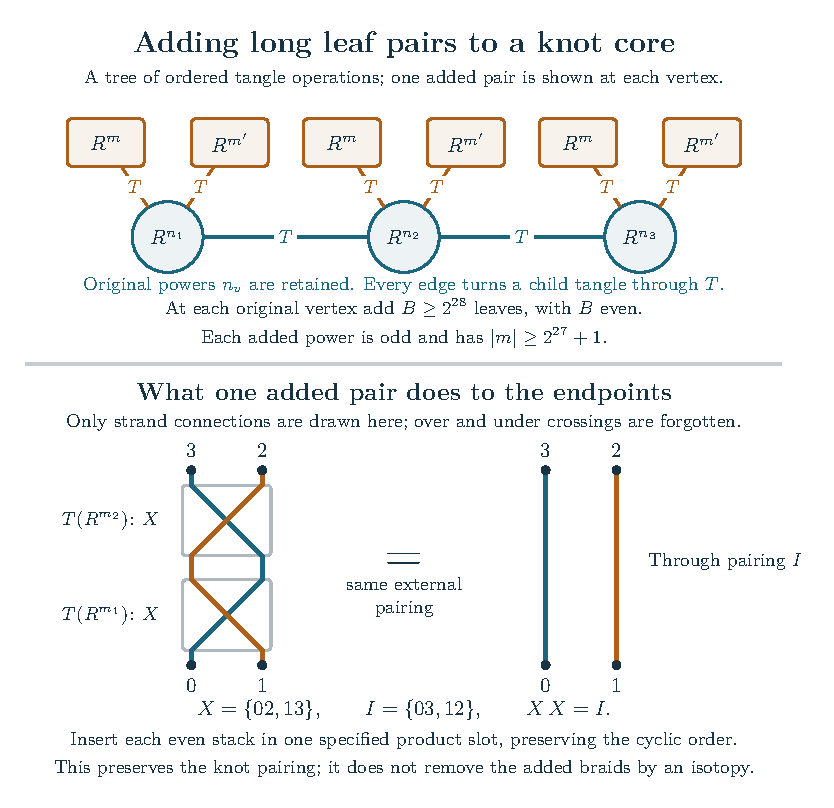
\includegraphics[width=.88\linewidth,height=.65\textheight,keepaspectratio]{../book/figures/directed-tree-volume.pdf}
\caption{Adding terminal pieces in pairs. The upper diagram records the tangle operations; only one of the required pairs is shown at each original vertex. Below, following the strands through two odd pieces gives two through connections. The endpoint pairing is preserved, while the knot type can change.}
\label{fig:directed-core-extension}
\end{figure}

\begin{corollary}\label{cor:directed-core-extension}
The resulting knot has a hyperbolic complement and satisfies
\eqref{eq:directed-volume} and \eqref{eq:directed-profile}.
The initial tree, all original powers, all inserted pieces and
their powers are fixed before $N$ tends to infinity.
\end{corollary}

This construction preserves the short-twist pieces and their endpoint
connections; it generally changes the knot. The corollary therefore
constructs a larger family of knots satisfying the volume identity.
It does not assert the identity for every unchanged short-twist
diagram from which the construction starts.

\section{A finite criterion beyond the simple bounds}

The choice of final vertex matters even with equal $c_v$. Consider
a star with $30{,}000{,}001$ terminal vertices. Give the center power
$2$ and each terminal vertex power $2^{60}+1$, and evaluate the
center last. The original strand calculation gives one knot.
For the center, exact rational bounds imply
\[
                   \frac{\beta_o}{\eta_o/2}<0.9.
\]
Its value of $\beta_o$ exceeds
$k_0(1-\cos r_0)$, so it cannot satisfy an outgoing condition for
any positive $c_o$. It need not do so because it is evaluated last.
The terminal vertices satisfy all their own conditions.

The summed test also fails for this example:
\[
 \sum_v\frac{d_v}{d_v^2+n_v^2}
 \ge\frac{30{,}000{,}001}{30{,}000{,}001^2+4}>2^{-25}.
\]
The example shows a precise benefit of the directed criterion.
Its size is deliberately conservative; no claim of a smallest such
example is needed. Appendix~\ref{app:directed-circle-messages}
gives the endpoint pairing calculation and the exact rational
inequalities, with a single reproduction command in
Chapter~\ref{ch:reproduction}.

\chapter{The geometric longitude selected by the finite source}
\label{gc:chapter}

The meridian profile contains more information than its first cusp
correction. For every covered fixed strict Conway tree with
independently sufficiently long signed twists, its full classical
characteristic is the preferred-longitude curve of the original
knot complement. Product junctions may have arbitrary valence and
may be adjacent. Ordered trees carrying a crossing circle at every
junction also retain their separate quantitative filling criteria.

We first establish the identity for the circle trees. Inserting a
circle around a zero-crossing box then supplies the geometric
extension to a bare product junction. Eliminating its angular
variable recovers the original stationary action with its constant,
while the ordered boundary paths recover the original knot group.
The consequence for a quantum recurrence uses the separate all-order
source theorem; the geometric statement alone supplies no new
asymptotic estimate for short fillings.

\section{The marked equations and their geometric branch}
\label{gc:equations}

Keep the literal construction of
Section~\ref{sec:circle-the-knot-construction}: one original crossing
circle at every vertex of a fixed finite ordered tree, at least one
edge, and an actual quarter-turn on every edge. The main strands must
form one knot, with no additional component closed inside a tangle.
All disk framings, endpoint orders and signed powers
$n_v=\epsilon_v-2p_v$ are retained.

Write $\mathcal E$ for the edge set. For an edge $e=vw$, let
$E_e=e^{2\pi i x_e}$ be its complex wire parameter, and put
$Q_v=e^{i\tau_v}$ at a crossing circle. These variables describe
the original cells, rather than a new diagram obtained by changing
the products. Let $M$ be the main meridian parameter. The selected
source flag has meridian eigenvalue $M^{-1}$; throughout this
chapter $L$ is the inverse eigenvalue of the preferred longitude
on that same flag. Equivalently, $(M,L)$ is the eigenvalue pair
on the other line of the determinant-one peripheral representation.

The finite source gives the rational equations
\begin{equation}\label{gc:edge}
\begin{aligned}
 &(E_e+Q_v)(E_e+Q_v^{-1})(E_e+Q_w)(E_e+Q_w^{-1})\\
 &\hspace{12mm}=(E_e-1)^2(1-E_eM^2)(1-E_e/M^2),
\end{aligned}
\end{equation}
\begin{equation}\label{gc:vertex}
 \prod_{e\ni v}\rho_{v,e}=Q_v^{n_v},
 \qquad
 \rho_{v,e}=\frac{Q_v+E_e}{1+Q_vE_e}.
\end{equation}
We use the chart on which these denominators are nonzero and the
selected critical point is nondegenerate, meaning that its Hessian
is invertible. Exponentiation alone
does not specify that point. To retain its logarithmic branch, put
\[
 b(x,\tau)=\int_0^x
       \log(2\cos(2\pi r)+2\cos\tau)\,dr-2J(x),
 \qquad J'(x)=\log(2\sin\pi x),
\]
with the original continued logarithms. The angular equations are
\begin{equation}\label{gc:first-charge}
 \sum_{e\ni v}b_\tau(x_e,\tau_v)
            +\frac{i n_v\tau_v}{2\pi}-i=0.
\end{equation}
The term $-i$ is the first Fourier charge of the actual crossing
trace. The positive charge path of the preceding geometric
completion starts at the complete augmented structure and ends
at this filled point. It identifies the source critical point
with the actual complete knot representation. The implicit-function
theorem then selects its continuation as $M$ varies near one.

\begin{theorem}[The preferred eigenvalue on the regular branch]
\label{gc:longitude-theorem}
Fix the construction above and a regular geometric branch through
an actual complete hyperbolic filling, with the logarithms selected
by \eqref{gc:first-charge}. On its continued germ,
\begin{equation}\label{gc:longitude}
 \boxed{\displaystyle
 L_{\mathrm{geom}}(M)
   =-M^{a(D)}
          \prod_{e\in\mathcal E}\frac{M^2-E_e(M)}
                                      {1-M^2E_e(M)},\qquad
 a(D)=-w(D)-\sum_vn_v .}
\end{equation}
Here $w(D)$ is the oriented writhe of the original filled diagram.
The longitude is its preferred zero-linking longitude, and the
representation is that of the original knot complement.
\end{theorem}

This theorem concerns a regular geometric branch. The long-filling
and quantitative hypotheses in the preceding chapters provide such
branches, with their stated knot and parity qualifications. They
remain the hypotheses for the corresponding volume limits; the
identification \eqref{gc:longitude} does not enlarge those analytic
claims.

\section{Why the equations describe the original exterior}
\label{gc:actual-exterior}

The attachment in Figure~\ref{fig:circle-octahedral-attachment}
is the topological starting point. Each original tree edge supplies
two octahedra. Their disk faces are sewn in the original cyclic
order, retaining the distinguished odd seam at each circle.
For a nonparabolic main meridian, both projection copies and their
white-face maps must deform. Keeping the old parabolic white maps
would give the wrong representation.

The resulting marked edge block satisfies \eqref{gc:edge}.
Its primitive auxiliary longitude has similarity $Q_v^2$,
and its meridian contribution is $\rho_{v,e}$.
The pure page identifications match both puncture generators.
At a positive half twist the actual ordered pair changes by
$(a,b)\mapsto(a^{-1}ba,a)$, preserving $ba$.
The invertible matrix $(ba)^{-1}-I$ realizes that conjugacy
near the geometric chart. The accompanying puncture flags must
also be transported: the two native ideal flags can select
opposite eigenvalues. The full generator matching, including
this exchange, is what permits gluing the actual collar.

Consequently the original primitive logarithms are
\begin{equation}\label{gc:primitive}
 U_v=\sum_{e\ni v}\log\rho_{v,e}-\epsilon_v\log Q_v,
 \qquad V_v=2\log Q_v,\qquad U_v+p_vV_v=-2\pi i.
\end{equation}
The last equality follows from the marked equation
\eqref{gc:first-charge}, since
$\exp(-2\pi b_\tau)=\rho_{v,e}$.
It retains the primitive period which disappears from
\eqref{gc:vertex}. The same ordered face and collar relations therefore construct
representations of the original augmented exterior. At the selected
filled point, $\operatorname{Im}\tau_v<0$, so $Q_v^2\ne1$.
The auxiliary longitude is noncentral and semisimple. Its commuting
filling word has eigenvalue ratio one by \eqref{gc:vertex}, and is
therefore projectively the identity. This proves descent to the
prescribed filled knot group, also on a sufficiently small nearby
germ. At $Q_v=\pm1$, an exponentiated slope equation alone would
not exclude a nontrivial parabolic filling word.

\section{From the peripheral differential to an exact identity}
\label{gc:rigidity}

There is a useful algebraic way to determine the entire longitude
without inferring it from a tangent. Put
$u=\log M$, $q_v=\log Q_v$, and
$f_e=(M^2-E_e)/(1-M^2E_e)$.
Differentiating the single edge equation gives
\begin{equation}\label{gc:edge-differential}
 du\wedge d\log f_e
 +\frac12 d\log\rho_{v,e}\wedge dq_v
 +\frac12 d\log\rho_{w,e}\wedge dq_w=0.
\end{equation}
The actual representation has the same boundary pairing:
\[
 du\wedge d\log L_{\mathrm{aug}}
       +\frac12\sum_v dU_v\wedge dq_v=0.
\]
Here $L_{\mathrm{aug}}$ uses the preferred augmented longitude.
This identity follows by pairing two infinitesimal representation
cocycles with the invariant trace form and evaluating their cup
product on the boundary of the exterior. The cochain Stokes
identity makes the total boundary evaluation zero. The factor
$1/2$ records that $U_v$ is a logarithm of an eigenvalue ratio.
Subtracting \eqref{gc:edge-differential} over all edges removes
the auxiliary terms in \eqref{gc:primitive}.

It follows that the rational squared discrepancy
\begin{equation}\label{gc:discrepancy}
 R=\frac{L_{\mathrm{aug}}^2}{\prod_e f_e^2}
\end{equation}
has no infinitesimal dependence on the auxiliary variables.
Two further facts turn that differential statement into an exact
formula. First, the generic source field has no extra algebraic
constants over $\mathbb C(M)$. Indeed its edge squareclasses are
\[
 (Q_v-1)^2(Q_w-1)^2
                 -4(M+M^{-1})^2Q_vQ_w.
\]
Each is an irreducible prime involving its own pair of vertex
variables. Their prime valuations make the squareclasses
independent, even after algebraically closing $\mathbb C(M)$.
Thus $R\in\mathbb C(M)$.

Second, at every fixed $M_0\ne0$ the group matrices and their
inverses admit a regular reconstruction for generic auxiliary
variables. This includes $M_0=\pm i$, where a particular ideal
subdivision degenerates but the character matrices remain regular.
The peripheral eigenvalue ratio and every $f_e$ are nonzero
there. Hence $R$ has neither a zero nor a pole on
$\mathbb C^*$, and therefore
\begin{equation}\label{gc:monomial}
                         R=cM^k
\end{equation}
for a nonzero constant $c$ and an integer $k$.
This regularity step is essential: a differential identity and a
single cusp derivative would not exclude a general rational
factor of $M$.

At the complete main cusp, $R(1)=1$. The already marked cusp
formula fixes $k=2a_{\mathrm{aug}}$, where
$a_{\mathrm{aug}}=-\sum_v\epsilon_v-w_\epsilon$.
The original surgery homology changes the preferred longitude by
$\mu_K^{\sum_vp_v\ell_v^2}$, with
$\ell_v\in\{0,\pm2\}$ the original circle linking numbers.
Its exponent is
\[
 a_{\mathrm{aug}}+\sum_vp_v\ell_v^2
             =-w(D)-\sum_vn_v=a(D).
\]
This proves the square of \eqref{gc:longitude}.

The remaining sign has a topological determination. A spin cover
is the double cover of oriented frames in which a full $2\pi$
rotation changes the lift's sign. On a Seifert
surface with one boundary component, a boundary-adapted tangent
frame winds $1-2g$ times relative to a global tangent frame.
The spin cover of that global frame has trivial boundary
monodromy, because the boundary is nullhomologous on the surface.
Thus the adapted frame lifts antiperiodically. At the straight
preferred cusp longitude it is the translation-invariant
horospherical frame; its positive unipotent lift therefore differs
from the actual longitude lift by a minus sign.
So $L_{\mathrm{geom}}(1)=-1$ at the complete filled point.
The two-valued holomorphic ambiguity in the squared identity is
constant, proving \eqref{gc:longitude}.
Appendix~\ref{app:geometric-characteristic} gives the marked
matrices, regularity argument and frame proof in full.

\section{Product junctions without crossing circles}
\label{gc:strict-extension}

A bare junction is a maximal consecutive product that contains no
crossing-circle operator. A binary association used to calculate its
kernel introduces hidden labels, but adds no physical quarter-turns.
The strict construction retains the original ordered products,
turns and cylindrical closure. Its real angle domain contains a
point at which every original leaf angle lies in $(0,1/2)$ and
every retained binary gate obeys
\[
                 \max(u,v)<w<u+v<1.
\]
The original endpoint test must give one knot, including any circles
closed inside a tangle. The two-leaf pure-leaf qualification and all
original parity conditions remain in force.

Let $\mathcal E_T$ denote the physical turn edges of the reduced
junction tree. Their covariant index $x_e$ is shared by the two ends
after lowering the trace pairing. When an incidence is exposed as
the ordinary output of its rooted branch, that output angle is
$1-x_e$. Put $X_e=e^{2\pi ix_e}$; this is the variable denoted $E_e$
in the preceding circle-tree formulas.

\begin{theorem}[The longitude for a strict Conway tree]
\label{gc:strict-longitude-theorem}
Fix such a strict ordered knot presentation and independently
sufficiently long signed powers, with the diagram and all its powers
fixed before the level varies. Its original complete hyperbolic
filled knot has a regular geometric main-meridian germ on which
\begin{equation}\label{gc:strict-longitude}
 L_{\mathrm{geom}}(M)
   =-M^{a(D)}\prod_{e\in\mathcal E_T}
           \frac{M^2-X_e(M)}{1-M^2X_e(M)},
 \qquad a(D)=-w(D)-\sum_i n_i.
\end{equation}
The $x_e(M)$ are selected by the original strict-tree action
continued with the physical-edge insertion
\begin{equation}\label{gc:strict-phase}
\begin{aligned}
 \Phi_t&=\Phi+\sum_{e\in\mathcal E_T}
       \{2J(x_e)-J(x_e+t)-J(x_e-t)\}
                 +\frac{\pi i a(D)}2t^2,\\
 &\hspace{32mm}M=e^{\pi it}.
\end{aligned}
\end{equation}
The preferred peripheral curves and the filled complement are those
of the original knot.
\end{theorem}

The proof begins with the framed collar in
Figure~\ref{fig:strict-zero-circle-junction}. Insert the literal
identity $R^0=I$ immediately before the ordered child product at
each bare junction, and encircle its two straight strands. Filling
that new circle along its primitive meridian restores the same
framed tangle. This operation creates no turn edge, crossing power
or preferred-longitude shear. It therefore leaves both
$\mathcal E_T$ and $a(D)$ unchanged.

There is a unique regular angular variable for each new circle.
If $x_1,\ldots,x_m$ are its incident covariant labels at the complete
strict optimizer, then $0<x_j\le1/2$, at most one label equals
$1/2$, and $\sum_jx_j>1$. With $k=\tanh(y/2)$, its zero-power
first-charge equation is
\begin{equation}\label{gc:zero-angular}
 \sum_j\arctan\bigl(k\tan\pi x_j\bigr)=\pi,
 \qquad \tau=-iy,\quad Q=e^y>1.
\end{equation}
A half label contributes $\pi/2$. The left side increases strictly
from zero or $\pi/2$ to $\pi\sum_jx_j$, so the solution exists,
is unique, and has a nonzero angular Hessian.

Let $V_m(\mathbf x)$ be the whole product action, after its original
hidden binary labels have been optimized. The exact elimination
identity is
\begin{equation}\label{gc:zero-legendre}
 V_m(\mathbf x)=\operatorname*{stat}_{\tau}
                  \left[\sum_j b(x_j,\tau)-i\tau\right].
\end{equation}
Both sides evaluate the same complete polynomial trace: one uses
the positive binary product, the other its first Fourier charge.
The constrained Laurent-coefficient calculation in
Appendix~\ref{app:strict-tree-geometric-characteristic} proves the
identity with its absolute constant. It continues holomorphically
through the possible half label.

The group marking requires a separate argument. In the fixed
product collar, the two based puncture loops satisfy
$a_{\mathrm{out}}=a_{\mathrm{in}}$ and
$b_{\mathrm{out}}=b_{\mathrm{in}}$, with disk-boundary word $ba$.
The complete old white-face maps identify the added primitive
longitude as $W_1^{-1}W_3$, up to its recorded orientation. Its
determinant-one normalization has trace $-(Q+Q^{-1})$, with
the same $Q>1$ as in \eqref{gc:zero-angular}. Pulling the old
holonomy back through the literal meridian-filling quotient keeps
both puncture generators and their paths. The resulting ordered
page conjugacies are the native all-circle conjugacies. Their
puncture pairs are irreducible, so the page intertwiners are unique
in the projective group. This identifies representations, including
the original odd seams, rather than matching only their traces.

At an internal half edge, $X_e=-1$ may be a double root of the
edge quadratic. The normalized character matrices remain regular.
One therefore retains the joint stationary system. The new angular
Hessian block is invertible; its Schur complement is exactly the
old strict reduced Hessian by \eqref{gc:zero-legendre}. The full
system is nondegenerate without inverting an individual edge
quadratic. Its rational longitude identity consequently extends
through this fold.

The selected added longitude remains semisimple near $Q>1$.
Its commuting meridian of eigenvalue ratio one is therefore
projectively identity, which removes the potential unipotent
ambiguity. The old marked deformation and sufficiently long
fillings identify the resulting main-meridian germ with that of
the original complete filled knot. Applying the all-circle
identity, and the same filled-knot Seifert sign, proves
\eqref{gc:strict-longitude}. No quantum estimate for the newly
drilled diagram is required; all quantum estimates remain those
of the original strict presentation.

\section{The resulting factor of a genuine quantum recurrence}
\label{gc:operator}

Now impose the all-order source hypotheses as well. They hold for
all the fixed strict Conway presentations in
Theorem~\ref{gc:strict-longitude-theorem} under independently
sufficiently long signed powers. For circle trees they also hold
under the summed condition
$\sum_vd_v/(d_v^2+n_v^2)\le2^{-25}$, or the local condition
$\max_vd_v/(d_v^2+n_v^2)\le2^{-120}$.
All original qualifications remain, and no data grow with the level.

Let $F_N(M)$ be the actual zero-framed reduced ADO state. A genuine
all-level annihilator means a fixed nonzero operator
\begin{equation}\label{gc:operator-definition}
 P(q,M,T)=\sum_{j=0}^d a_j(q,M)T^j,\qquad
 TM=qMT,\qquad
 P(q_N,M,T)F_N(M)=0
\end{equation}
at every sufficiently large level, where
$q_N=e^{\pi i/N}$ and $T$ shifts $M$ to $q_NM$.
The coefficients $a_j$ belong to $\mathbb C(q,M)$.
Clear its fixed rational denominators and remove the common
$q-1$ order. Setting $q=1$ and replacing the shift by a
commuting variable $L$ gives its first nonzero classical symbol
$P_0(M,L)$.

The all-order theorem in Appendix~\ref{app:filtered-characteristic}
uses the actual source on the translated microscopic charts
$s,s+1,\ldots,s+d$, away from ordinary resonances.
Its filtered logarithm selects the critical-value germ
$L_{\mathrm{eff}}=-e^{\mathcal S'(\log M)}$.
The exact edge insertion gives the right side of
\eqref{gc:strict-longitude}, with the original physical edge set.
The marked first-charge branch and the zero-circle elimination
fix the same filled representation. Theorems~\ref{gc:longitude-theorem}
and~\ref{gc:strict-longitude-theorem} therefore identify
$L_{\mathrm{eff}}$ with $L_{\mathrm{geom}}$ in their respective
source classes.

The reduced/full conversion retains its meridian factor: before
formal-domain cancellation the classical equation is
\begin{equation}\label{gc:meridian-factor}
 (M-M^{-1})^d P_0(M,L_{\mathrm{geom}}(M))=0.
\end{equation}
It follows that $P_0$ vanishes on the geometric germ.
Let $A_{\mathrm{geom},\mathbb C}$ be the irreducible Laurent
polynomial defining the smallest complex algebraic curve containing
this geometric eigenvalue germ. Then
\begin{equation}\label{gc:factor}
                     A_{\mathrm{geom},\mathbb C}\mid P_0.
\end{equation}
If $a_j\in\mathbb Q(q,M)$, one instead contracts the prime of
that germ to
$\mathbb Q[M^{\pm1},L^{\pm1}]$; the chosen complex component
need not itself be defined over $\mathbb Q$.

This is a selected geometric factor of every specified annihilator
under the source hypotheses. It does not identify the whole
classical symbol, the full A-polynomial, or the entire annihilator
ideal. Nor does it give a fixed-$M\ne1$ quantum asymptotic by
substituting $s$ of order $N$. The full geometric germ is obtained
from all orders on fixed microscopic charts and the separate
marked representation argument above.

\section{Transfer under an ordered reduction of the presentation}
\label{gc:intrinsic-transfer}

The reduced ADO function and the preferred eigenvalue germ belong
to the marked, zero-framed knot. Suppose the existing ordered
net-twist reduction gives an ambient isotopy from the input to a
covered strict presentation. The isotopy carries the knot
orientation, positive meridian, preferred zero-linking longitude
and cut mark. After correcting the transported ribbon framing to
zero, the full function $F_N(M)$ agrees at every level, as does
its rational continuation. Any genuine annihilator of that
intrinsic family therefore has the factor in \eqref{gc:factor}.
Presentation-specific recurrence formulas need not agree.

The same conclusion applies to an arbitrary-closure reduction
when it produces one covered strict knot factor and only unknot
factors. Under the reduction theorem's long surviving-factor
hypotheses, a hyperbolic knot input has precisely that form.
Removing the exhibited unknot summands is an ambient isotopy,
and its exterior map carries the preferred peripheral pair.
No assertion about quantum-growth multiplicativity for connected
sums is used here.

For a fixed original expression there are finitely many reduction
and parity branches. Taking the maximum of their strict source
and geometric thresholds gives a uniform sufficient threshold
for the surviving signed net powers. Large powers that cancel
to a short net power do not satisfy this condition. The integer
$a(D)$ and the edge factors are computed on the covered strict
diagram; only their preferred-longitude product and the selected
geometric factor are transferred intrinsically. The full proof
and precise reduction references are in
Section~\ref{gj:transfer-to-presentations-with-net-twists-and-arbitrary-closures}.

\chapter{Checking the certificates and understanding the scope}\label{ch:reproduction}

The volume theorems combine written analytic and geometric arguments with finite checks of different kinds. The long-twist proof reduces two local inequalities to exact rational certificates supplied with the paper. The quantitative circle-tree proof establishes its uniform bounds analytically; separate finite checks verify its edge formulas, face identifications and peripheral identities. This chapter distinguishes those roles and records the scope of each theorem.

\section{Three different kinds of evidence}
The manuscript contains analytic proofs, exact finite certificates, and optional finite audits. They have different logical roles. The matrix identities, support and strictness arguments, geometric incidence, complex estimates and filling analysis are proved in the text. The rational certificates are finite parts of the proof: the continuum inequalities reduce to their exact feasibility, coverage and supporting-plane checks. Finite matrix or numerical asymptotic audits provide independent checks of formulas and normalizations, but do not establish a theorem by extrapolation.

The proof is given in the chapters and appendices of this manuscript. The repository also supplies the exact certificate data and verification programs. Those programs check the finite inequalities described below; they do not formally verify the analytic or geometric arguments.

\section{Replaying the exact certificates}
From the repository root, run
\begin{verbatim}
python3 repro/verify.py --output repro/results
\end{verbatim}
The serial runner uses the standard Python library. It replays the two-leaf block certificate, the attachment square certificate and the optional endpoint certificate, compares their exact results with the recorded data, and checks the elementary rational leaf and isolated-three-leaf margins. Its report records the source and data hashes. Candidate generation and numerical optimization are not run by verification.

The principal proof files are
\begin{center}\small
\begin{tabular}{p{0.44\textwidth}p{0.46\textwidth}}\toprule
Certificate & Mathematical coverage\\\midrule
\path{verify_conway_two_leaf_block_alias_certificate.py}
& Sixteen slope intervals; both alias types; 288 corner/vertex inequalities.\\[5pt]
\path{verify_conway_single_leaf_attachment_certificate.py}
& Exact 55-rectangle cover; 880 corner/vertex inequalities on the full child/parent slope square.\\[5pt]
Endpoint certificate in the runner's manifest
& Optional stronger margin at the monotone-response endpoint; not needed for the main theorem.\\\bottomrule
\end{tabular}
\end{center}
All paths are resolved relative to the repository or script directory, rather than an author's temporary working directory. The runner's proof-input guide lists the written dependencies separately from executable checks.

\section{Checking the quantitative tree formulas}
The elementary edge equations and complex-strip estimates used by Chapter~\ref{ch:quantitative-circle-trees} have a portable reproduction command:
\begin{verbatim}
python3 repro/run_research_checks.py curvature-fillings
\end{verbatim}
The runner checks exact symbolic edge identities, finite samples of the stated complex inequality, labeled octahedral attachments and the full signed peripheral matrix words. Its output separates those computations from the uniform analytic and geometric proofs. Appendix~\ref{app:quantitative-sums} gives the full quantitative finite-sum proof, including both uniform Newton estimates, the weighted contraction and the charge-tail bounds. Appendix~\ref{app:quantitative-geometry} gives the complete ordered attachment, positive angular charts, primitive-period completion, volume calibration and preferred-cusp argument. The linked versions are optional separately available copies of those proofs. Such finite checks can detect sign or indexing errors; they do not replace the written proofs.

\section{The planar terminal decoration}
The finite identities for Chapter~\ref{ch:balanced-terminal-fans} have one command:
\begin{verbatim}
python3 repro/run_research_checks.py balanced-terminal-fans
\end{verbatim}
The script uses exact integer and rational arithmetic. It checks the
closed fan recurrence, the rational balance margin, the oriented
triangle subdivision and its new ordered quadrilateral, the matching
and even-level face parity, and the endpoint pairing of even stacks of
odd terminal tangles. It does not infer an asymptotic theorem from
sampled quantum values. Appendix~\ref{app:balanced-terminal-fans}
proves the geometric realization, full finite source, uniform
Fourier estimates and primitive completion.

\section{The directed criterion and unmarked junctions}

The exact rational comparisons for
Chapter~\ref{ch:directed-circle-messages} have one command:
\begin{verbatim}
python3 repro/run_research_checks.py directed-tree-fillings
\end{verbatim}
This program uses only Python's standard library. It verifies the
constant inequalities for the uniform twist bound and the star with
central power two, using rational enclosures of all quantities.
The uniform conditional kernel estimate, induction over arbitrary
fixed trees, noncancellation and geometric interpretation are written
proofs in Appendix~\ref{app:directed-circle-messages}.

For the local algebra of the unmarked-junction extension, run
\begin{verbatim}
python3 repro/run_research_checks.py strict-tree-geometry
\end{verbatim}
This program requires SymPy. It checks the white-map normalizations,
primitive disk-longitude trace, incident radius formulas and the
half-angle fold identity. Appendix~\ref{app:strict-tree-geometric-characteristic}
proves the based boundary-map comparison, stationary elimination and
full representation assembly. Those global statements are not
deduced from the finite matrix checks.

\section{Building the manuscript and illustrated guide}
The TeX source is in \sourcefile{manuscript/}; its native illustrations are in \sourcefile{manuscript/figures/}. A TeX Live or MacTeX installation with \sourcefile{latexmk} builds the paper:
\begin{verbatim}
python3 tools/build_manuscript.py
\end{verbatim}
The output is \sourcefile{manuscript/build/main.pdf}. The build manifest records the hashes of all TeX and bibliography inputs and the generated PDF. It is a typesetting record, not a mathematical certificate.

The illustrated guide is built separately:
\begin{verbatim}
python3 tools/build_book.py
python3 tools/check_book.py
\end{verbatim}
It is written to \sourcefile{docs/} and links the same authored PDF. Documentation builds do not execute research scripts. The guide also links the broader research companions and states their hypotheses separately from the two theorem classes developed here.

\section{What has and has not been proved}
Theorem~\ref{thm:main} is uniform in the level for each fixed finite completed expression and each fixed sufficiently long signed filling tuple. It includes both parity sequences and composite levels. Its threshold can depend on the expression, its complete geometry and its retained half-twist pattern, but imposes no bound on ratios between the long slopes.

Theorem~\ref{thm:circle-quantitative} uses a different sufficient hypothesis: the literal ordered circle tree and the explicit sum $\sum_vd_v/(d_v^2+n_v^2)\le2^{-25}$. The full diagram, all degrees and all integer powers are fixed before the limit. The theorem gives actual hyperbolicity and volume equality, a uniform microscopic meridian profile with its exact scalar, and the preferred-cusp correction. It permits short coefficients under this condition; it does not prove a statement about arbitrary short or rational fillings.

Both results keep the original strand order, knot-pairing test, disk framings and unfilled main cusp. The octahedral attachment is proved by actual labeled cuts. A scalar equality in $\cH_N$ is not used as a tangle isotopy. The continued boundary word used for the preferred-cusp calculation becomes the preferred longitude of the smooth filled knot only at the endpoint of the geometric path.

These are sufficient construction hypotheses, not a classification of all arborescent knots. The completed-box condition remains part of Theorem~\ref{thm:main}; the quarter-index states in circle trees are treated by the separate proof in Chapter~\ref{ch:quantitative-circle-trees}. More general strict ordered Conway trees have a long-twist theorem in the linked research companions, with their own full source and marked-geometry proofs. No general short-filling theorem follows merely from the existence of complete augmented cells or from an upper bound on the absolute values of a larger sum.

\section{The geometric longitude calculation}
The symbolic identities in the geometric characteristic chapter have one
reproduction command:
\begin{verbatim}
python3 repro/run_research_checks.py geometric-characteristic
\end{verbatim}
This group requires SymPy. It verifies the nonparabolic face maps,
character matrices, half-twist line transports, and the differential
and discriminant formulas. The topological gluing, boundary pairing,
algebraic constants and regularity arguments remain the written proofs
of Appendices~\ref{app:filtered-characteristic} and
\ref{app:geometric-characteristic}.


\section{Uniform bounds for inserting twists}
Appendix~\ref{app:uniform-filling-bound} proves a level-independent
bound for each original filling functional, measured against the
supremum of the shared spectral polynomial. Its finite identities
can be checked with one command:
\begin{verbatim}
python3 repro/run_research_checks.py filling-supremum
\end{verbatim}
This group requires SymPy and NumPy. It checks the derivative
interpolation and Chebyshev residues exactly, then compares the
functional with independently constructed signed crossing matrices
over finite fields. The shared exponential estimate remains a
separate hypothesis; these checks add no new volume class.

\appendix
\chapter{Finite algebra and normalization identities}\label{app:finite}

This appendix proves the finite identities on which the asymptotic argument rests. The first calculation compares the chosen crossing matrices and reduced trace with the conventional invariant. The next two calculations establish the Newton basis, its genuine geometric turn, and the exact color decomposition. The last calculation expands an arbitrary twist power while keeping derivatives at repeated roots. No limiting argument is used in these identities.

\section{The crossing comparison and enhancement}\label{app:normalization}
This section supplies the finite normalization calculation used in Proposition~\ref{prop:normalization}. Put $\omega=Q$ and
\[
 p_j=\prod_{h=1}^{j}(1-\omega^h),\qquad
 \bar p_j=\prod_{h=1}^{j}(1-\omega^{-h}),\qquad p_0=1.
\]
Kashaev's unbraided four-index matrix may be written by introducing nonnegative residues
\[
 u=[j-i-1],\quad v=[i-l],\quad t=[l-k],\quad h=[k-j].
\]
Its support conditions are equivalent to $u+v+t+h=N-1$, and on that support
\begin{equation}\label{eq:A-original-crossing}
 R^o_{(i,j);(k,l)}=
 \frac{N\omega^{1-(t+h)(u+h)}}{p_u\bar p_vp_t\bar p_h}.
\end{equation}
One free $j$ and such a composition specify one entry. Let $F_{ij}=\omega^{ij}/\sqrt N$. Its full Fourier transform has only the ordinary-integer-conserving entries
\begin{equation}\label{eq:A-Fourier-crossing}
 ((F^{-1}\otimes F^{-1})R^o(F\otimes F))_{(a-k,b+k);(a,b)}
 =\omega^{1+(a-k)(b+1)}\frac{p_ap_{b+k}}{p_{a-k}p_bp_k},
\end{equation}
for $0\le k\le\min(a,N-1-b)$.

Here is the finite summation. Define
\[
 S_m(X)=\sum_{j=0}^m\frac{X^j}{p_j\bar p_{m-j}}
 =\frac{\prod_{j=1}^m(X-\omega^j)}{p_m}.
\]
The equality follows by induction from $\bar p_m=(-1)^m\omega^{-m(m+1)/2}p_m$ and
$(1-\omega^m)S_m=(X-\omega^m)S_{m-1}$. The free Fourier index imposes conservation modulo $N$. The two remaining factors are
$S_{N-1-z}(\omega^{c-z})S_z(\omega^{z-a})$; their zeros force $c\le z\le a$. With $m=a-c$, the residual sum is
\[
 \omega^{1+c(b+1)}\frac{p_a}{p_c}
 \sum_{j=0}^m\frac{(-1)^j\omega^{j(j-1)/2}\omega^{(b+1)j}}
 {p_jp_{m-j}}
 =\omega^{1+c(b+1)}\frac{p_a}{p_c}
 \frac{(\omega^{b+1};\omega)_m}{p_m}.
\]
If $b+m\ge N$, the product contains $1-\omega^N$ and vanishes. Otherwise it is $p_{b+m}/p_b$, proving \eqref{eq:A-Fourier-crossing} with integer, rather than merely residue, conservation.

Set $G_j=p_j/(1-\omega)^j=q^{j(j-1)/2}[j]_q!$, $D_j=(-q)^j$, and $\gamma=\omega q^{-d^2/2}$. Substitution into \eqref{eq:universal-crossing} gives exactly
\[
 (F^{-1}\otimes F^{-1})R^o(F\otimes F)
 =\gamma(DG\otimes G)\mathscr R(G^{-1}\otimes G^{-1}D^{-1}).
\]
For the enhanced braid conventions take
\[
 B_K=P(R^o)^T,\quad\mu_K=-qS,\quad\alpha_K=-q,
 \qquad B_q=P\mathscr R^T,\quad\mu_q=K^{-1},\quad
 \alpha_q=q^{(N^2-1)/2},
\]
where $S v_j=v_{j+1\bmod N}$. On $b$ strands, the single similarity
\[
 U_b=F^{-\otimes b}\bigotimes_{j=1}^b(G^{-1}D^{j-1})
\]
works for every adjacent generator because the quantum crossing conserves integer weight and commutes with $D\otimes D$. It also sends $\mu_q^{\otimes b}$ to $\mu_K^{\otimes b}$, and $\gamma\alpha_q=\alpha_K$. The writhe characters cancel exactly. The partial traces commute with the remaining module generators; distinct $K$ weights and nonzero $F$ arrows imply scalarity. Thus every internal similarity cancels, including the one open factor of a reduced cut. This proves the finite enhanced comparison used in Chapter~\ref{ch:source}. Large factorial gauges are never estimated by their norms.

The primal/dual change of basis is $Bv_j=(-1)^jq^{j(j-N)}v_{d-j}$. Direct generator substitution conjugates $K^{-1}$ to the primal pivot and the crossing to the recorded primal convention. At completeness $g_{\rm ADO}=(-1)^dK$ and the twist has the corresponding sign. A $b$-strand closure of writhe $w$ and $c$ components has $w\equiv b-c\pmod2$, so the remaining enhancement ratio is $(-1)^{d(c-1)}$. Its modulus is one, and for a knot it is one in this convention.

\section{The block polynomial and the physical Newton turn}\label{app:newton}
For completeness we justify the block minimal polynomial used in Lemma~\ref{lem:commutant}. Before specialization, the ordinary highest-weight module of highest weight $d$ has weights $d-2a$. In the pair, a highest vector of total degree $j$ is obtained by solving the bidiagonal raising equation. If its coefficient at $|a,j-a\rangle$ is $u_a$, the equation at $|a,j-a-1\rangle$ determines $u_{a+1}/u_a$ as the negative ratio of the two nonzero raising entries. Thus for generic $q$ there is one such vector in each degree $j=0,\ldots,d$. Its highest weight is $2d-2j$, its Casimir is $q^{2d-2j+1}+q^{-2d+2j-1}$, and its successive lowering vectors are nonzero through the usual length. The dimensions $2d-2j+1$ sum to $N^2$. Distinct generic Casimirs make these submodules independent.

In degree $T\le d$, precisely the highest vectors $j\le T$ contribute one descendant each. Their eigenvalues give the block characteristic polynomial. At $q=e^{\pi\ii/N}$ it becomes
\[
 \prod_{j=0}^{T}(z-c_j),\qquad c_j=q^{2j+1}+q^{-2j-1}.
\]
All physical matrix entries specialize regularly. The nonzero adjacent entries of the tridiagonal block make a boundary vector cyclic, so this characteristic polynomial is also minimal even when roots coincide. At $T=d$ it is $P_N$. The elementary identity
\[
 \prod_{j=0}^{N-1}(z-q^{2j+1}-q^{-2j-1})=2T_N(z/2)+2
\]
can also be checked by putting $z=w+w^{-1}$: the roots correspond to $w^N=-1$, and the monic degree and leading coefficient agree. The generating property of $W_d$ propagates its vanishing to the full pair.

Now $B_r(\Omega)$ annihilates every degree block $W_T$ with $T<r$, with multiplicities, and has first-color bandwidth at most $r$. In the turned matrix its first-color displacement is $d-(a+b)$, so $\Turn B_r$ annihilates every $W_T$ with $T<d-r$. Its representing polynomial is therefore divisible by $B_{d-r}$.

For the reverse degree bound, its first middle-block column is
\[
 (\Turn B_r)_{a0}=x^{a-d}(B_r(\Omega))_{(d-a,0);(d-a,0)},
\]
which vanishes for $a>d-r$. A polynomial of degree $k<N$ in the cyclic tridiagonal middle block has a nonzero $k$th coordinate on the first basis vector, from its unique outermost path. Thus $\deg\Turn B_r\le d-r$, proving $\Turn B_r=C_rB_{d-r}$.

Use the physical entry from $(d-r,0)$ to $(0,d-r)$. On the turned side it is the unique $r$-step path in the high-degree block, whose factors are
\[
 Q^{j-r}(1-Q^{r-j})(1-Q^{j+1}),\qquad0\le j<r.
\]
Including the leading coefficient $(-1)^r$ gives $s_r^2$. The corresponding path for $B_{d-r}$ in the low block gives $s_{d-r}^2$. All turn monomials in this entry equal one. Hence
\[
 \Turn B_r=\frac{s_r^2}{s_{d-r}^2}B_{d-r},
 \qquad \Turn\Bhat_r=\Bhat_{d-r}.
\]
Finally $s_rs_{d-r}=N$ and \eqref{eq:leading-trace} give
$\phi(\Bhat_i\Bhat_j)=\delta_{i+j,d}$: use degree below $d$, leading coefficient at $d$, and full divisibility by $P_N$ above it. This proves Proposition~\ref{prop:newton-turn} by physical support and exact paths.

\section{Circle coefficients and the signed alias}\label{app:colors}

We derive the coefficient formulas rather than infer them from values at the distinct Casimir roots. That distinction is necessary because the quotient algebra also contains first derivatives at double roots. The generating-function calculation first gives a polynomial identity at a generic parameter; regular specialization then retains all those derivatives automatically.
The generic Chebyshev--Newton identity is
\begin{equation}\label{eq:A-Cheb-newton}
 U_{j-1}(z/2)=\sum_{r=0}^{j-1}(-1)^r
 \genfrac{[}{]}{0pt}{}{j+r}{2r+1}_q B_r(z).
\end{equation}
To prove it, successively divide
$1-zt+t^2=(1-c_rt+t^2)+t(c_r-z)$. The formal identity is
\[
 \frac1{1-zt+t^2}
 =\sum_{r\ge0}\frac{(-t)^rB_r(z)}{\prod_{i=0}^{r}(1-c_it+t^2)}.
\]
After $r$ steps the remainder is divisible by $t^{r+1}$. The denominator factors as a consecutive $q$-string, and the Gaussian Pascal recurrence gives its reciprocal coefficient. Taking the coefficient of $t^{j-1}$ gives \eqref{eq:A-Cheb-newton}. For $j\le\lfloor N/2\rfloor$, every factorial index is below $N$; specializing and turning proves \eqref{eq:low-alias}.

For higher colors use the polynomial identity
\[
 U_{N-h-1}=\tfrac12(\Cheb_hU_{N-1}-\Cheb_NU_{h-1}).
\]
Since $\Cheb_N=-2$ in the full algebra,
\[
 L_{N-h}=(-1)^h\tfrac12\Cheb_hL_N+(-1)^NL_h.
\]
The $v$th turned coefficient of the first term is
$(-1)^hN\sum_{k=0}^{d}\cos(h(2k+1)\pi/N)\Bhat_v(c_k)$.
This finite sum can be evaluated without a zero denominator. Put $z=w+w^{-1}$. The factorization of $B_v$ is the consecutive string
\[
 B_v(w+w^{-1})=(-1)^vw^{-v}
 \prod_{j=0}^{2v-1}\left(w-q^{-(2v-1)+2j}\right).
\]
For $0\le v,h\le M$, all its Fourier exponents after multiplication by $w^{\pm h}$ have absolute value below $N$. Summing at $w=q^{2k+1}$ extracts only the constant coefficient. The finite Gaussian product gives that coefficient as zero for $v<h$, and as
$(-1)^h s_{2v}/(s_{v-h}s_{v+h})$ for $v\ge h$. Dividing by $s_v^2$ and multiplying the two factors of $N$ proves \eqref{eq:core-alias}, including $h=0$ and both parities.

For the half twist, multiplication by $z$ in Newton coordinates is the lower bidiagonal matrix $Z$ with $Z_{rr}=c_r$ and $Z_{r+1,r}=-4\sin^2((r+1)\pi/N)$. The one-crossing matrix is
\[
 (R(Z))_{ij}=\kappa(-1)^iq^{i(j+1)}\frac{s_i}{s_js_{i-j}},\qquad i\ge j.
\]
Its first column is the finite Newton expansion of the crossing. Substituting the two neighboring ratios shows that it commutes with $Z$; since the first coordinate is cyclic, this determines the full matrix. Reversal on both sides gives \eqref{eq:half-twist}. Coefficient conjugation gives the inverse crossing because its full Hermite values and logarithmic derivatives are conjugate. This argument retains all normal directions.

\section{Fourier--Hermite interpolation of an arbitrary twist}\label{app:fourier}

Ordinary interpolation prescribes values. Hermite interpolation also prescribes derivatives at a repeated node. Here the crossing power supplies both data, and the change of variable $z=w+w^{-1}$ turns the interpolation problem into a finite Fourier calculation. The two Fourier equations below solve simultaneously for the coefficients that ordinary value interpolation would fail to distinguish.
For an integer $\ell$, let $f_{N,\ell}$ be the degree-below-$N$ remainder of $r_N^\ell$ modulo $P_N$. Negative powers exist because all its nodal values are nonzero. At $w_k=q^{2k+1}$ define
\[
 h_k=\bigl((-1)^kq^{k(k+1)}\bigr)^\ell,
 \qquad d_k=-\frac\ell2(d-2k)h_k.
\]
At a double node, $d_k=(w_k-w_k^{-1})f_{N,\ell}'(c_k)$; at the odd simple node both sides of the logarithmic derivative condition vanish without prescribing an extra derivative. Put
\[
 H_n=\frac1N\sum_kh_kw_k^{-n},\qquad
 D_n=\frac1N\sum_kd_kw_k^{-n},\qquad0\le n<N.
\]
Then
\begin{equation}\label{eq:A-Hermite-Fourier}
 f_{N,\ell}(z)=a_0+\sum_{n=1}^{d}a_n\Cheb_n(z),\qquad
 a_0=H_0,\quad a_n=\frac{D_n+(N-n)H_n}{N}.
\end{equation}
Indeed the Laurent polynomial $f(w+w^{-1})$ has symmetric coefficients $a_n$ at $w^{\pm n}$. At $w_k^N=-1$ its values and logarithmic derivatives have aliases
\[
 H_n=a_n-a_{N-n},\qquad
 D_n=na_n+(N-n)a_{N-n}.
\]
Solving gives \eqref{eq:A-Hermite-Fourier}. At the even middle index $H_{N/2}=0$ and the derivative equation still determines the coefficient. Paired nodes give the required compatibility, and the odd simple root imposes exactly one condition. Thus no root or normal is omitted.

Set $a_N=a_{N+1}=0$ and
\[
 \beta_j^{\ell/2}=(-1)^j(a_j-a_{j+2}),\qquad0\le j<N.
\]
The identity $\Cheb_n=U_n-U_{n-2}$ gives the circle expansion. Since $|h_k|=1$ and $|d_k|\le|\ell|N/2$, one has $|a_0|\le1$, $|a_n|\le1+|\ell|/2$, and
\[
 \sum_j|\beta_j^{\ell/2}|\le2N(1+|\ell|/2).
\]
For $\ell=2P$, these are the coefficients used in \eqref{eq:sampled-derivative}. To obtain that formula directly, substitute the two finite Fourier sums into $a_j-a_{j+2}$, set $j=N-h-1$, and pair $h$ with $-h$ in an even corridor. The difference of the two exponentials gives $\sinh(2\pi\ii z_k)$; the differentiated data give the linear factor $2PNz_k+h$, and differentiating the hyperbolic sine gives its cosine. Their sum is precisely $U_N'(z_k)/(2\pi\ii)$. The constant phase is $(-1)^d\kappa^{-P}$ and the two averaging factors give $N^{-2}$. This verifies \eqref{eq:sampled-derivative} with both normal terms and both parity conventions.

\chapter{Detailed estimates for the color sums and filling contours}\label{app:analytic}

The local and global estimates have different purposes. Section~\ref{app:selected-source} constructs an exponentially accurate holomorphic approximation on the strict neighborhood used for the saddle. Section~\ref{app:global-core-envelope} bounds every remaining core coefficient, including parameters where the recurrence eigenvalues meet. The last section treats the joining contours for the filling integral. Keeping these estimates separate prevents a local asymptotic expansion from being applied outside its proven domain.
\section{The exact local recurrence and its holomorphic asymptotic}
\label{app:selected-source}

This section proves the local source estimate used in the completed-root
theorem. Its hypothesis is a fixed compact interval
\begin{equation}\label{eq:b1-high-interval}
 I=[\tau_0,\tau_1]\subset(1/4,1/2)
\end{equation}
for every retained complete leaf coordinate. All constants may depend on
this interval and the fixed source tree. The color neighborhood and every
complex index neighborhood below are fixed independently of the level.
We work with the actual finite low core and its specified factorial
continuation. No homogeneous solution of a recurrence is substituted for
that source. In particular, an inverse-power approximation on the real
index grid will not be used as if it were an exponentially accurate
complex interpolation.

\subsection{Canonical factorials and the literal mixed coefficient}

To move a color parameter off the integer grid, we must specify a function that agrees with the finite coefficient and preserves its phase. The Gamma product below supplies that function for the sine factorials. Its exact shift identity will then allow the finite recurrence to remain valid at complex colors; agreement only in a leading asymptotic term would not be sufficient.

Retain
\[
 d=N-1,\quad M=\lfloor d/2\rfloor,\quad
 q=e^{\pi\ii/N},\quad Q=q^2,\quad \kappa=q^{d^2/2},\quad
 F_r=(Q;Q)_r.
\]
In this section $x$ denotes a scaled Newton index, rather than the
physical-frame scalar $q^d$. The sine factorial has the exact continuation
\begin{equation}\label{eq:b1-factorial}
 G_N(z)=\left(\frac{2\pi}{N}\right)^z\Gamma(z+1)
 \prod_{k=1}^{\infty}
 \frac{\Gamma(Nk+z+1)}{\Gamma(Nk-z)(Nk)^{2z+1}},
 \qquad -1<\Re z<N.
\end{equation}
All positive-base powers use their real logarithms. The logarithm of the
$k$th factor is $O_K(k^{-2})$ on compact subsets of the strip: in the
Gamma-ratio expansion its $k^{-1}$ term cancels. Thus the product is
holomorphic and zero-free there. Gamma's functional equation and the
convergent sine product give
\begin{equation}\label{eq:b1-factorial-shift}
 \frac{G_N(z+1)}{G_N(z)}=2\sin\frac{\pi(z+1)}N,
 \qquad G_N(0)=1,\qquad G_N(r)=s_r\quad(0\le r<N).
\end{equation}
The marked quantum factorial is
\begin{equation}\label{eq:b1-marked-factorial}
 \widehat F_N(z)=
 e^{\pi\ii z(z+1)/(2N)-\pi\ii z/2}G_N(z).
\end{equation}
Consequently
\[
 \widehat F_N(z+1)=(1-Q^{z+1})\widehat F_N(z),
 \qquad \widehat F_N(r)=F_r,
 \qquad Q^z=e^{2\pi\ii z/N}.
\]
These identities fix the continuation and its phase, not just its
asymptotic expansion. On a compact subset of $0<\Re z<1$, direct
Stirling expansion of \eqref{eq:b1-factorial} gives
\begin{equation}\label{eq:b1-factorial-asymptotic}
 \begin{aligned}
 \log G_N(Nz)
 &=NJ(z)+\frac12\operatorname{Log}(2N\sin\pi z)
   +\frac{\pi\cot\pi z}{12N}+O(N^{-3}),\\
 J(z)&=\int_0^z\operatorname{Log}(2\sin\pi u)\,\dd u.
 \end{aligned}
\end{equation}
Here the logarithm continues the real positive factorial branch. One
way to verify the uniform remainder is to expand the $k$th Gamma ratio:
its error is $O_K(N^{-3}k^{-3})$. These errors are summable; the
leading and half-log terms sum by the sine product. The first correction
sums by
\[
 z^{-1}+\sum_{k\ge1}\bigl((k+z)^{-1}-(k-z)^{-1}\bigr)
 =\pi\cot\pi z.
\]
Cauchy's estimate supplies the corresponding derivative bounds on
smaller compact sets.

Let $h$ be a physical color deficit and put $t=h/N$. At an integer
index $r>h$ the pure core coefficient is the literal factorial expression
\begin{equation}\label{eq:b1-pure-coefficient}
 A_N(r,t)=\frac{N^2s_{2r}}
 {s_r^2G_N(r-Nt)G_N(r+Nt)}.
\end{equation}
For a retained half-twist sign $\eps\in\{1,-1\}$, the exact triangular
Newton transport gives
\begin{equation}\label{eq:b1-signed-finite}
 d_N^\eps(r,t)=\kappa^\eps
 \sum_{v=r}^{M}(-1)^v q^{\eps v(r+1)}
 \frac{s_v}{s_rs_{v-r}} A_N(v,t),
 \qquad d_N^0(r,t)=A_N(r,t).
\end{equation}
For complex $t$ in a sufficiently small fixed disk, only the two
color-shifted factorials are continued. All their arguments remain in
regular strips. Equation \eqref{eq:b1-signed-finite} is then an exact
finite, even holomorphic function. At every physical integer $h<r$ it
is the original transported core, including all first normal directions.

The cancellation inside this finite sum is encoded by
\begin{align}
 A_{h,r}
 &=\sum_{v=r}^{M}
 \frac{Q^{-vr}F_{2v}}
 {F_v\widehat F_N(v-h)\widehat F_N(v+h)F_{v-r}},
 \label{eq:b1-A-source}\\
 D_{h,r}
 &=\frac{Q^{-r^2}F_{2r}}
 {F_r\widehat F_N(r-h)\widehat F_N(r+h)},
 \qquad U_{h,r}=A_{h,r}/D_{h,r}.
 \label{eq:b1-D-source}
\end{align}
The sum starts at $r$ in the present corridor. For physical $r<h$ its
lower endpoint would be $h$; those low indices belong to the separate
global envelope, not to the interpolation asserted here. The terminal
source in \eqref{eq:b1-D-source} is exactly $U_{h,M}=1$.

\subsection{Deriving the recurrence, including its endpoint}

The identity traditionally called a Ward equation here is simply a second-order recurrence obtained by telescoping the actual finite sum. A recurrence has many solutions, so we include its upper endpoint condition in the derivation. That condition is what selects the coefficient occurring in the invariant.

Put $H=Q^h=e^{2\pi\ii t}$, $T_h=H+H^{-1}$ and $Y=Q^r$. The
literal finite sum satisfies
\begin{multline}\label{eq:b1-Ward}
 QY^2(1-Q^2Y)A_{h,r+2}
 +Y(T_hQ^3Y^2+Q+1)A_{h,r+1}\\
 -Q(QY+1)(QY^2-1)A_{h,r}=0,
 \qquad A_{h,M+1}=0.
\end{multline}
Here and below an absent term beyond the finite upper support is zero.
We give the summation certificate, since the endpoint fixes which
solution of this second-order equation is the physical one.

For the summand of \eqref{eq:b1-A-source}, write $z=Q^v$. Its ratio
under $v\mapsto v+1$ is
\[
 \frac{Y^{-1}(1-Qz^2)(1+Qz)}
 {(1-Qz/H)(1-QHz)(1-Qz/Y)}.
\]
Use the rational certificate
\[
 g_h(z)=\frac{(1-z/H)(1-Hz)(1-z/Y)}{z^2}.
\]
The telescoping difference, divided by the original summand, is
\begin{equation}\label{eq:b1-Ward-certificate}
 \left(\frac1{YQ^2}-1\right)z^{-2}
 +\left(\frac1{YQ}+H+H^{-1}+\frac1Y\right)z^{-1}
 -\frac1{YQ}-1-\frac{H+H^{-1}}Y.
\end{equation}
The lower endpoint has $z=Y$ and hence vanishes. The upper endpoint
contains $F_{2M+2}=0$. The ratio for the shift $r\mapsto r+1$ is
$z^{-1}-Y^{-1}$. Expressing the first two $z^{-1}$ moments in terms of
$A_{h,r+1}$ and $A_{h,r+2}$ in
\eqref{eq:b1-Ward-certificate} gives \eqref{eq:b1-Ward} by multiplication
of its displayed denominators. This argument remains exact for complex
$h=Nt$: the shifted factorial equations are exact and the lower zero
is still $z=Y$. It does not use interpolation from finitely many colors.

Normalize by the actual $D_{h,r}$ and set
\[
 \operatorname{den}_r=(1-QY/H)(1-QYH).
\]
Then
\begin{equation}\label{eq:b1-normalized-recurrence}
 U_r=p_N(r,t)U_{r+1}+q_N(r,t)U_{r+2},
\end{equation}
where the exact rational coefficients are
\begin{align}
 p_N&=-\frac{Q^{-2}Y^{-1}(T_hQ^3Y^2+Q+1)}
                 {\operatorname{den}_r},
 \label{eq:b1-p-coefficient}\\
 q_N&=-\frac{Q^{-4}Y^{-2}(1-Q^2Y)(1-Q^3Y^2)(1+Q^2Y)}
 {\operatorname{den}_r\operatorname{den}_{r+1}}.
 \label{eq:b1-q-coefficient}
\end{align}
All these denominators are bounded away from zero on the corridor used
below. At the last recurrence row one has the exact wall
\begin{equation}\label{eq:b1-wall}
 q_N(M-1,t)=0,
 \qquad U_{M-1}=p_N(M-1,t),\qquad U_M=1.
\end{equation}
For odd $N=2m+1$, $M=m$ and the factor $1-Q^3Y^2$ vanishes.
For even $N=2m$, $M=m-1$ and $1+Q^2Y$ vanishes.
The zero is independent of $H$. In particular no nonexistent
$D_{h,M+1}$ is divided out and no arbitrary terminal ratio is imposed.

\subsection{The selected analytic root and a source-exact continued fraction}

We solve the recurrence backwards from its finite upper endpoint. On the strict high-index interval, one characteristic root dominates the other. The resulting contraction permits a holomorphic continued fraction. Crucially, an exact zero in the last recurrence row erases the artificial tail of this continued fraction, so it agrees with the original finite solution on the integer grid.

Regard \eqref{eq:b1-p-coefficient}--\eqref{eq:b1-q-coefficient} as
holomorphic functions $p(x,t,\varepsilon_N)$ and
$q_c(x,t,\varepsilon_N)$, where
$\varepsilon_N=N^{-1}$, $Y=e^{2\pi\ii x}$ and
$Q=e^{2\pi\ii\varepsilon_N}$. At $\varepsilon_N=0$, put
\begin{equation}\label{eq:b1-leading-recurrence}
 \begin{split}
 D_t&=(1-Y/H)(1-YH),\\
 p_0&=-Y^{-1}\frac{(H+H^{-1})Y^2+2}{D_t},\qquad
 q_0=-Y^{-2}\frac{(1-Y^2)^2}{D_t^2}.
 \end{split}
\end{equation}
The two roots of $\mu^2-p_0\mu-q_0=0$ at $t=0$ are
\begin{equation}\label{eq:b1-two-roots}
 \mu_s(x,0)=-Y^{-1},\qquad
 \mu_f(x,0)=Y^{-1}\cot^2(\pi x).
\end{equation}
On a compact real interval in $(1/4,3/4)$ containing
$[\tau_0,1/2]$, the selected branch $\mu=\mu_s$ is nonzero,
$\Re\mu>0$, and $|\mu_f/\mu|<1$. The same inequalities, with uniform
strict constants, hold on a fixed complex neighborhood and a sufficiently
small complex $t$ disk. Indeed at $t=0$ these assertions follow directly
from \eqref{eq:b1-two-roots}; nonvanishing and a separated quadratic root
persist on a small complex thickening. Write
\begin{equation}\label{eq:b1-dominance}
 \left|\frac{\mu_f}{\mu}\right|\le k_0<1,
 \qquad \Re\mu\ge m_0>0.
\end{equation}
The endpoint $x=1/2$ is included. Direct substitution gives
$\mu(1/2,t)=1$, while $q_0$ has a double zero there and its first
$\varepsilon_N$ derivative also vanishes. The selected root and its
normalization are regular at the physical terminal point.

Choose $\sigma_0>0$ so small that
$[\tau_0-\sigma_0,1-\tau_0+4\sigma_0]\subset(1/4,3/4)$.
Use a fixed complex neighborhood of this larger interval on which
\eqref{eq:b1-dominance} holds, and put
\[
 \mathcal L_N=\left\lceil(1/2-\tau_0+2\sigma_0)N\right\rceil,
 \qquad \mathcal F_x(z)=p(x,t,\varepsilon_N)
                  +\frac{q_c(x,t,\varepsilon_N)}z.
\]
Define the finite continued fraction
\begin{equation}\label{eq:b1-ratio-interpolant}
 v_N(x,t)=\mathcal F_x\circ\mathcal F_{x+\varepsilon_N}\circ
 \cdots\circ\mathcal F_{x+(\mathcal L_N-1)\varepsilon_N}
 \bigl(\mu(x+\mathcal L_N\varepsilon_N,t)\bigr).
\end{equation}
This is defined on a fixed complex neighborhood of $[\tau_0,1/2]$.
For a constant $C$ independent of $N$, the disks of radius
$C\varepsilon_N$ around the respective selected roots are invariant
under backward iteration. To prove this, note first that
\[
 \mathcal F_x(\mu(x+\varepsilon_N,t))-\mu(x,t)
 =O(\varepsilon_N).
\]
On those disks the derivative in the continued-fraction argument has
modulus at most $k_0+O(\varepsilon_N)$. Choose $k_1\in(k_0,1)$ and then
$C$ so that the $O(\varepsilon_N)$ error plus
$k_1C\varepsilon_N$ is at most $C\varepsilon_N$. This proves the
invariance inductively. The disks avoid zero, so every iterate is
holomorphic, nonzero, and has uniformly bounded inverse. In particular
\begin{equation}\label{eq:b1-ratio-leading}
 v_N(x,t)=\mu(x,t)+O(N^{-1})
\end{equation}
uniformly holomorphically on a fixed smaller domain.

At a physical $x=r/N$, the continued fraction reaches the row $M-1$.
By \eqref{eq:b1-wall}, that row forgets its entire remaining tail and
takes exactly the value $p_N(M-1,t)$. Backward induction from the literal
source $U_M=1$ therefore proves
\begin{equation}\label{eq:b1-exact-ratio}
 v_N(r/N,t)=\frac{U_{Nt,r}}{U_{Nt,r+1}},
 \qquad \tau_0N\le r<M.
\end{equation}
This also proves that the displayed physical source values are nonzero.
The equality holds uniformly for complex $t$ in the fixed disk. There is
no assertion about a nonexistent physical ratio at $r=M$.

Adding one more future step to \eqref{eq:b1-ratio-interpolant} changes
the future value by $O(\varepsilon_N)$, and the preceding
$\mathcal L_N$ contractions reduce that change by $k_1^{\mathcal L_N}$.
Thus its Riccati defect is exponentially small. This explains why the
analytic tail used to define the interpolant cannot hide a macroscopic
change of the original source.

\subsection{First transport correction and absolute amplitude normalization}

Let $p_1=\partial_{\varepsilon}p|_{\varepsilon=0}$ and
$q_1=\partial_{\varepsilon}q_c|_{\varepsilon=0}$, differentiating the
explicit rational coefficients. Define
\begin{equation}\label{eq:b1-nu}
 \nu=\frac{p_1+q_1/\mu-q_0\mu_x/\mu^2}
                  {1+q_0/\mu^2}.
\end{equation}
The denominator is $1-\mu_f/\mu$, bounded away from zero by
\eqref{eq:b1-dominance}. Substitution of
$\mu+\varepsilon_N\nu$ into the one-step Riccati equation gives a
residual $O(\varepsilon_N^2)$. The same contracting backward iteration
then gives
\begin{equation}\label{eq:b1-ratio-first}
 v_N=\mu+N^{-1}\nu+O(N^{-2})
\end{equation}
on a fixed smaller complex neighborhood. For example, subtract the
trial iterate from the exact one at each step. The resulting error is
bounded by the geometric sum of its $O(N^{-2})$ local defects and the
contracted terminal discrepancy. Cauchy estimates give the corresponding
uniform derivative expansions.

Use the logarithm with positive real part in
\eqref{eq:b1-dominance}, continuing from $\mu(1/2,t)=1$, and set
\begin{equation}\label{eq:b1-action-amplitude}
 \begin{split}
 S(x,t)&=\int_x^{1/2}\operatorname{Log}\mu(u,t)\,\dd u,\\
 C(x,t)&=\sqrt{\mu(x,t)}
 \exp\left(\int_x^{1/2}\frac{\nu(u,t)}{\mu(u,t)}\,\dd u\right).
 \end{split}
\end{equation}
The square root is one at $1/2$. The integral branches are fixed by the
actual selected source; $C$ is holomorphic and nonzero.

Summing logarithms of the exact ratios in
\eqref{eq:b1-exact-ratio}, using \eqref{eq:b1-ratio-first} and the first
Euler--Maclaurin endpoint term, gives
\begin{equation}\label{eq:b1-U-leading}
 U_{Nt,r}=C(r/N,t)e^{NS(r/N,t)}[1+O(N^{-1})].
\end{equation}
The product stops at $M-1$, because $U_M=1$. Replacing the true endpoint
$M/N$ by $1/2$ costs only $O(N^{-1})$: the displacement is $O(N^{-1})$
at either parity, and $\operatorname{Log}\mu(1/2,t)=0$. The remaining
endpoint terms in the correction are likewise $O(N^{-1})$. In
particular there is no free terminal matching constant.

At $t=0$, direct differentiation of
\eqref{eq:b1-p-coefficient}--\eqref{eq:b1-q-coefficient} yields
\[
 \operatorname{Log}\mu=\pi\ii-2\pi\ii x,
 \qquad \frac\nu\mu=-\frac\pi2\cot(\pi x)-\frac{5\pi\ii}2.
\]
Therefore
\begin{equation}\label{eq:b1-complete-calibration}
 S(x,0)=\pi\ii(1/2-x)^2,\qquad
 C(x,0)=\sqrt{\sin\pi x}\,
                 e^{-3\pi\ii(1/2-x)/2}.
\end{equation}
This calculation fixes the absolute amplitude from the finite source,
rather than from the value of an unknown closed invariant.

\subsection{Exponential interpolation before an oscillatory saddle}

Equation \eqref{eq:b1-U-leading} is not sufficient by itself for a
complex wire saddle. Its relative error is only inverse polynomial and
could exceed a fixed oscillatory cancellation. The exact ratio
\eqref{eq:b1-exact-ratio} supplies the needed stronger estimate.

Put $f_N(x,t)=\operatorname{Log}v_N(x,t)$ and $b_N=M/N$.
On a fixed larger complex tube the $f_N$ are uniformly bounded and
holomorphic. On an inner tube, Cauchy's estimate gives constants
$B,a>0$, independent of $N,t$, such that
\begin{equation}\label{eq:b1-Cauchy}
 |\partial_x^k f_N(x,t)|\le Bk!a^{-k}.
\end{equation}
For $K_N=\lfloor c_aN\rfloor$, with a sufficiently small fixed
$c_a>0$, form the holomorphic expression
\begin{align}
 E_N(x,t)
 &=N\int_x^{b_N}f_N(u,t)\,\dd u
       +\frac{f_N(x,t)-f_N(b_N,t)}2
 \notag\\
 &\quad+\sum_{k=1}^{K_N}
 \frac{B_{2k}}{(2k)!}N^{1-2k}
 \bigl[\partial_x^{2k-1}f_N(b_N,t)
       -\partial_x^{2k-1}f_N(x,t)\bigr].
 \label{eq:b1-optimal-EM}
\end{align}
The Bernoulli polynomial bound
$|B_{2k}(u)|\le4(2k)!/(2\pi)^{2k}$ together with
\eqref{eq:b1-Cauchy} bounds the Euler--Maclaurin remainder by
\[
 C N\left(\frac{K_N}{\pi aN}\right)^{2K_N}
 \le C e^{-cN}
\]
after decreasing $c_a$. This is uniform in the complex color disk and
on the physical high grid. Since the product of the exact ratios is
precisely $U_r$, it follows that
\begin{equation}\label{eq:b1-exponential-grid}
 U_{Nt,r}=e^{E_N(r/N,t)}[1+R_{N,r}(t)],
 \qquad |R_{N,r}(t)|\le C e^{-cN}.
\end{equation}
The empty terminal product equals one. The residual is retained as a
source term, rather than reinterpreted as a homogeneous solution.

The same explicit expression is holomorphic in the index $x$.
Using \eqref{eq:b1-ratio-first} in
\eqref{eq:b1-optimal-EM}, the higher Bernoulli terms sum to $O(N^{-1})$
on an inner fixed tube, and hence
\begin{equation}\label{eq:b1-interpolant-leading}
 e^{E_N(x,t)}=C(x,t)e^{NS(x,t)}[1+O(N^{-1})]
\end{equation}
uniformly holomorphically. Equations
\eqref{eq:b1-exponential-grid} and
\eqref{eq:b1-interpolant-leading} have distinct roles: the former is
an exponentially accurate comparison with the original finite source,
and the latter is a leading expansion of a specified complex function.

\subsection{Keeping the quadratic phase and determining the signed action}

The half-twist coefficient contains a quadratic exponential in the color. Such a phase is sometimes called a chirp. Its continuation is part of the finite formula, not an arbitrary choice of interpolation. We now combine it with the recurrence solution and the continued factorials; this calculation determines the local action and the nonzero amplitude used in the saddle.

Remove only the known external phase by defining
\[
 \ell_N^\eps(r,t)=e^{-\ii\eps\pi d/4}d_N^\eps(r,t),
 \qquad \eta_N=\exp\left(\frac{\ii\pi d}4
                               \sum_{\ell}\eps_\ell\right).
\]
The positive sign is the coefficientwise conjugate of the negative sign
on real parameters. Its holomorphic continuation uses Schwarz
reflection, not conjugation of a free holomorphic variable.

The original factorial phase gives the exact identity
\begin{equation}\label{eq:b1-color-phase}
 q^{h^2}\frac{D_{h,r}}{D_{0,r}}
 =\frac{G_N(r)^2}{G_N(r-h)G_N(r+h)}.
\end{equation}
It follows immediately from \eqref{eq:b1-marked-factorial}; the linear
and quadratic exponents in the two shifted arguments must both be kept.
Combining \eqref{eq:b1-signed-finite}--\eqref{eq:b1-D-source} with
\eqref{eq:b1-color-phase} gives the negative-sign interpolant
\begin{align}
 A_N^{\rm hol}(x,t)
 &=\frac{N^2G_N(2Nx)}
 {G_N(Nx)^2G_N(N(x-t))G_N(N(x+t))},
 \notag\\
 \nu_N(z)&=e^{-\pi\ii z+\pi\ii z(z+1)/N},
 \qquad P_N^{\rm ch}(x)=\frac{\kappa^{-1}e^{\pi\ii d/4}}{\nu_N(Nx)},
 \notag\\
 I_N^-(x,t)&=A_N^{\rm hol}(x,t)P_N^{\rm ch}(x)e^{E_N(x,t)}.
 \label{eq:b1-signed-interpolant}
\end{align}
The superscript on $P_N^{\rm ch}$ distinguishes this chirp factor from
the Casimir polynomial. At every integer $r$,
$\nu_N(r)=(-1)^rq^{r(r+1)}$. Its displayed analytic continuation is
fixed before any contour deformation. In particular,
\begin{equation}\label{eq:b1-chirp-cancellation}
 P_N^{\rm ch}(x)e^{NS(x,0)}
   =e^{\pi\ii(3/4-x-1/(2N))}.
\end{equation}
Changing the continuation of $(-1)^r$ would change a lattice frequency;
that change is not permitted. Equation
\eqref{eq:b1-exponential-grid} proves that
$I_N^-(r/N,t)$ agrees with the actual $\ell_N^-(r,t)$ up to a
relative exponential residual. For the positive sign set
$I_N^+(x,t)=\overline{I_N^-(\bar x,\bar t)}$; for the pure sign use
$I_N^0=A_N^{\rm hol}$, which agrees exactly on the grid.

Define
\begin{align}
 g(x,t)&=J(2x)-2J(x)-J(x-t)-J(x+t),
 \notag\\
 f_0(x,t)&=g(x,t),\qquad
 f_-(x,t)=g(x,t)+S(x,t)-S(x,0),
 \notag\\
 f_+(x,t)&=\overline{f_-(\bar x,\bar t)}.
 \label{eq:b1-local-actions}
\end{align}
The factorial expansion and \eqref{eq:b1-chirp-cancellation} yield
\begin{equation}\label{eq:b1-local-asymptotic}
 I_N^\eps(x,t)=N^{1/2}b_\eps(x,t)e^{Nf_\eps(x,t)}
                                      [1+O(N^{-1})],
\end{equation}
uniformly holomorphically on fixed smaller domains, with
\begin{align}
 b_0(x,t)&=
 \frac{\sqrt{\sin(2\pi x)}}
 {2^{3/2}\sin(\pi x)
       \sqrt{\sin(\pi(x-t))\sin(\pi(x+t))}},
 \notag\\
 b_-(x,t)&=b_0(x,t)e^{\pi\ii(3/4-x)}C(x,t),\qquad
 b_+(x,t)=\overline{b_-(\bar x,\bar t)}.
 \label{eq:b1-local-amplitudes}
\end{align}
All square roots continue their positive complete factorial branches.
At completeness,
\begin{equation}\label{eq:b1-amplitude-at-zero}
 \frac{b_\eps(x,0)}{b_0(x,0)}
 =\sqrt{\sin(\pi x)}e^{-\ii\eps\pi x/2},
 \qquad \eps\in\{-1,1\}.
\end{equation}
These factors are nonzero. The remaining $e^{-\pi\ii/(2N)}$ in
\eqref{eq:b1-chirp-cancellation} belongs to the stated inverse-power
error; it is not an omitted constant or parity phase.

\subsection{An exact source action identity and its Hessian}

The action above can also be characterized without integrating the
quadratic root. For each physical sign $\eps\in\{0,1,-1\}$ solve
near $s=t=0$ the equation
\begin{equation}\label{eq:b1-shear}
 t=s-\frac{\eps}{2\pi\ii}g_s(x,s).
\end{equation}
Its $s$ derivative at zero is $1-\eps\ii\cot(\pi x)$, which is
nonzero. Then the source-selected action satisfies
\begin{equation}\label{eq:b1-shear-action}
 f_\eps(x,t)=g(x,s)-\frac{\eps}{4\pi\ii}g_s(x,s)^2,
 \qquad (f_\eps)_x=g_x(x,s),\qquad (f_\eps)_t=g_s(x,s).
\end{equation}
The derivative identities follow by differentiating
\eqref{eq:b1-shear}. To identify the value with the actual selected
source, consider the negative sign. Put
$E=e^{2\pi\ii x}$, $H=e^{2\pi\ii t}$ and $T=e^{2\pi\ii s}$.
Exponentiating \eqref{eq:b1-shear} gives
\[
 H=\frac{T(E-T)}{ET-1},\qquad
 T^2+E(H-1)T-H=0,
 \qquad T=1\text{ at }H=1.
\]
For $K=e^{-g_x(x,s)}=-(1-E/T)(1-ET)/(1+E)^2$, elimination of $T$
gives
\begin{equation}\label{eq:b1-action-polynomial}
 K^2(1+E)^2+K[(H+H^{-1})E^2+2]+(1-E)^2=0.
\end{equation}
On the other hand \eqref{eq:b1-local-actions} and the selected quadratic
give $e^{-(f_-)_x}=E\mu D_t/(1+E)^2$, satisfying exactly
\eqref{eq:b1-action-polynomial}. At $H=1$, both constructions take
the branch $K=\tan^2(\pi x)$; their logarithms agree by their complete
marks. Hence their $x$ derivatives agree. The possible remaining function
of $t$ is zero by the limit $x\to1/2$: there $S=0$,
$J(1/2+t)=-J(1/2-t)$, and the implicit shear has $s=t$, $g_s=0$.
Schwarz reflection proves the positive sign. This fixes the source
action, not merely a Hessian with the same entries.

In particular, all local actions are even in $t$, equal $g(x,0)$ at
zero, and
\begin{equation}\label{eq:b1-local-hessian}
 (f_\eps)_{tt}(x,0)
 =-\frac{2\pi\cot(\pi x)}{1-\eps\ii\cot(\pi x)},
 \qquad \eps\in\{0,1,-1\}.
\end{equation}
Their real parts are strictly negative on the fixed high interval.

\subsection{The exact finite wire window and its lattice saddle}
\label{app:lattice-laplace}

We now specify the function to which the complex saddle argument is
applied. Let the fixed completed-root expression have $H$ leaves and
$K=2H-3$ primitive free integer wires. The last forced product is removed
using its exact relation $i+j=d$, whose coefficient is one. Every
remaining wire has the affine form
\[
 r_w=NL_w(y)+\delta_w,
 \qquad y=k/N,\quad k\in\ZZ^K,
\]
where the integer offsets $\delta_w$ are fixed by the original compiler.
Take a small fixed rectangular window $B$ about the strict complete
optimizer. All leaf coordinates lie in intervals of the form
\eqref{eq:b1-high-interval}, and every retained gate inequality is
strict on a fixed neighborhood of the closure of $B$.

The exact finite window is
\begin{equation}\label{eq:b1-exact-window}
 \mathcal C_N(\mathbf t)
 =\sum_{k/N\in B}
  \prod_{\ell=1}^{H}\ell_N^{\eps_\ell}(r_\ell,t_\ell)
  \prod_{g=1}^{H-2}\mu_N(r_{g,1},r_{g,2},r_{g,3}).
\end{equation}
Its support is independent of the complex colors. It is a finite,
separately even holomorphic function. For all sufficiently large $N$,
every state in this window is a true core state at every physical small
color deficit. The factors $\mu_N$ are the original positive Newton
coefficients, not their leading asymptotic replacements.

Replace each exact local factor by its canonical holomorphic
interpolant only after keeping its residual. The gate interpolation is
the same seven-factorial expression with $G_N$, and agrees exactly on
its integer grid. For the signed leaves, use
\eqref{eq:b1-signed-interpolant}. The total error in the finite sum is
bounded absolutely by
\begin{equation}\label{eq:b1-grid-error-before-saddle}
 \poly(N)\exp\{N(F_0+C\|\mathbf t\|^2-c)\}
\end{equation}
for some fixed $c>0$. Indeed there are polynomially many states, all
actions are even analytic perturbations of the common complete real
action, and the relative leaf errors in
\eqref{eq:b1-exponential-grid} are exponentially small. This estimate
is made before any oscillatory cancellation. Shrink the fixed color
polydisk so that \eqref{eq:b1-grid-error-before-saddle} is exponentially
below the nearby selected critical action.

The interpolated summand has phase
\begin{equation}\label{eq:b1-wire-phase}
 \mathcal F(y,\mathbf t)
 =\sum_{\ell}f_{\eps_\ell}(L_\ell(y),t_\ell)
  +\sum_g m(L_{g,1}(y),L_{g,2}(y),L_{g,3}(y)).
\end{equation}
At zero color it is the original complete action. Its wire Hessian at
the strict optimizer is negative definite. Thus it has one holomorphic
critical branch $y_*(\mathbf t)$, with
\[
 \Phi(\mathbf t)=\mathcal F(y_*(\mathbf t),\mathbf t).
\]
The local gate amplitude is
\[
 b_\mu(x,y,z)=2^{-3/2}
 \sqrt{\frac{\sin\pi(x+y)\sin\pi z}
 {\sin\pi x\sin\pi y\sin\pi(z-x)\sin\pi(z-y)\sin\pi(x+y-z)}}.
\]
Multiply all leaf and gate amplitudes by the exact leading offset factor
\begin{equation}\label{eq:b1-offset-factor}
 \exp\left[
  \sum_\ell\delta_\ell\partial_x f_{\eps_\ell}
  +\sum_g\nabla m(L_g(y))\mathbin{\cdot}\delta_g\right]
\end{equation}
to obtain the nonzero holomorphic density $b_E(y,\mathbf t)$.
The changed $f_\eps$ is used in \eqref{eq:b1-offset-factor}, including
at nonzero complex color; a pure offset factor would be incorrect.
The interpolated summand is
\[
 N^{3-H}b_E(y,\mathbf t)e^{N\mathcal F(y,\mathbf t)}
 [1+O(N^{-1})].
\]

For clarity we give the finite-lattice contour step. Choose the vertical
faces of the rectangle at half-grid values. In each coordinate the exact
summation kernel is $\pi N\cot(\pi Nz)$, with residue one at $z=k/N$.
On a vertical half-grid line, $|\cot(\pi Nz)|\le1$. Those faces lie
away from the strict real optimizer and retain a fixed phase gap.
On a horizontal line of fixed height $a>0$, the cotangent differs from
its constant value $\mp\ii$ by $O(e^{-2\pi Na})$. At complete color,
the real part of the phase grows under this small imaginary displacement
by at most $Ca^2$; the even color perturbation costs at most
$C\|\mathbf t\|^2$. Choose $a$ so $Ca^2<\pi a$, and then choose the
color polydisk small enough. Every nonconstant kernel term has an
exponential gap, including all side connectors. Applying this argument
successively in the $K$ primitive coordinates retains the full product
contour and its orientations. The constant horizontal terms give
$N^K$ times the ordinary integral. Replacing the moving half-grid
rectangle by $B$ costs only exponentially small boundary strips.

Translate that integral to the nearby complex critical point. The
endpoint connectors remain below its action, and the real tangent
Gaussian is uniformly nondegenerate. Extend its local Gaussian range
with exponentially small error. The odd first correction integrates to
zero, giving a relative $O(N^{-1})$ expansion. Thus
\begin{equation}\label{eq:b1-window-asymptotic}
 \mathcal C_N(\mathbf t)
 =N^{3/2}a_E(\mathbf t)e^{N\Phi(\mathbf t)}[1+O(N^{-1})],
 \qquad
 a_E(\mathbf t)=\frac{(2\pi)^{K/2}b_E(y_*(\mathbf t),\mathbf t)}
                    {\sqrt{\det[-\mathcal F_{yy}(y_*(\mathbf t),\mathbf t)]}}.
\end{equation}
The determinant square root is selected from the positive complete
Gaussian. The power is
$3-H+K/2=3/2$. The exponential grid error
\eqref{eq:b1-grid-error-before-saddle} is smaller than this answer by
the prior choice of color disk, and is added back only now. Both level
parities have the same primitive density and displayed normalization.

At completeness,
\begin{equation}\label{eq:b1-global-amplitude}
 \Phi(0)=F_0,\qquad
 a_E(0)=a_E^{\rm pure}(0)
 \prod_{\eps_\ell\ne0}
   \sqrt{\sin(\pi x_{\ell,*})}e^{-\ii\eps_\ell\pi x_{\ell,*}/2}\ne0.
\end{equation}
Evenness gives $\mathcal F_{yt_\ell}(y,0)=0$, so the wire Schur
correction to the color Hessian vanishes. With
$c_\ell=\cot(\pi x_{\ell,*})$, one obtains
\begin{equation}\label{eq:b1-global-hessian}
 \partial_{t_\ell}\partial_{t_j}\Phi(0)
 =-\frac{2\pi c_\ell}{1-\eps_\ell\ii c_\ell}\delta_{\ell j}
 =2\pi\ii\tau_\ell\delta_{\ell j},
 \qquad \tau_\ell=\frac{\ii c_\ell}{1-\eps_\ell\ii c_\ell},
 \qquad \Im\tau_\ell>0.
\end{equation}
On a smaller fixed complex box,
\begin{equation}\label{eq:b1-finite-packet-envelope}
 |\mathcal C_N(u+\ii v)|
 \le\poly(N)e^{N(F_0-a\|u\|^2+B\|v\|^2)},\qquad a>0.
\end{equation}
This bound is for the exact finite function
\eqref{eq:b1-exact-window}, by
\eqref{eq:b1-window-asymptotic}, not just its leading formal action.

\subsection{Returning from the local sum to the original evaluation}

We finish by stating precisely how the independent alias estimates are
used. The compositional proof in the main text gives a uniform positive
gap for every nonempty alias sector on the entire physical color cube.
It also gives a concave all-core majorant with the unique strict complete
maximizer used above. The latter uniqueness is global: it agrees with the
strict complete action near that point, and a second maximum of a concave
function would give a constant segment through that strictly concave
neighborhood.

Hence all core states outside the fixed wire window have a fixed gap,
uniformly in physical colors. Within that window the actual local
far-color recurrence estimate loses a fixed positive amount whenever
one physical deficit exceeds a fixed small corridor. Polynomial state
counting and the finite number of sectors therefore give constants
$\delta,\gamma>0$ such that the literal mixed scalar $\mathcal A_N$ obeys
\begin{align}
 \max_{0\le h_\ell\le\delta N}
 \left|\mathcal A_N(\mathbf h)-
          \eta_N\mathcal C_N(\mathbf h/N)\right|
 &\le\poly(N)e^{N(F_0-\gamma)},
 \label{eq:b1-source-restoration}\\
 \max_{\exists\ell:\,h_\ell>\delta N}
 |\mathcal A_N(\mathbf h)|
 &\le\poly(N)e^{N(F_0-\gamma)}.
 \label{eq:b1-color-complement}
\end{align}
The maximum in the second line is over the entire original physical
color cube, not just the low-core band. No alias is folded into the even
analytic packet. The external $\eta_N$ is exactly the retained unit
phase defined above.

The global coherent-core input here is its uniform exponential-rate
envelope, of the form $\exp\{N(\widetilde g+o(1))\}$ with the
$o(1)$ uniform over all physical indices and colors. It is not a
polynomial-prefactor assertion through every spectral collision.
To obtain \eqref{eq:b1-source-restoration}--\eqref{eq:b1-color-complement},
first fix the strictly positive variational and far-color margins, then
absorb the uniform $o(N)$ errors into, for example, half their minimum.
Polynomial counting and the remaining finite prefactors are harmless
after that reduction of $\gamma$. The polynomial-prefactor local packet
proved above is a separate estimate on its fixed regular high interval.

These estimates preserve the whole-source remainder through the finite
filling sum. For each fixed signed filling tuple, the exact Hermite
coefficient bound is $\sum_j|\beta_{j-1}^{-p_\ell}|\le2N(1+|p_\ell|)$.
Thus \eqref{eq:b1-source-restoration} and
\eqref{eq:b1-color-complement} incur only a polynomial multiplier in
that whole sum. The finite analytic packet, rather than its pointwise
leading approximation, is then used for the Fourier endpoint and charge
arguments. Its exact evenness, complex estimate
\eqref{eq:b1-finite-packet-envelope}, nonzero amplitude and Hessian
\eqref{eq:b1-global-hessian} are the needed inputs. The retained filling
analysis supplies the smaller filled action and a nonzero leading
coefficient; the source gap is not itself a replacement for that analysis.

The argument in this section requires
\eqref{eq:b1-high-interval}. No continuation through a quarter-index
dominance boundary, no additional root-leaf closure, and no theorem for
arbitrary tangle syntax is used in the manuscript's completed-root result.

\section{A uniform global envelope through the source collisions}
\label{app:global-core-envelope}

The local interpolation of Section~\ref{app:selected-source} is used
only on a fixed high-index interval. Here we prove the different estimate
needed before restricting to that interval: a uniform exponential-rate
bound for every physical color and every core index. The proof retains
the other recurrence branch, including its repeated-root colors.
Here $C_j^\eps$ always denotes the core polynomial of a single physical
leaf of color $j$ and half-twist sign $\eps$, as in
\eqref{eq:core-alias}; it does not denote the whole analytic packet.

\subsection{The complete-diagonal normalization and its literal wall}

Use $q,Q,d,M,F_r$ as in Section~\ref{app:selected-source}. For a physical
integer $0\le h\le M$, interpret the finite sum $A_{h,r}$ in
\eqref{eq:b1-A-source} with lower endpoint $\max(r,h)$. Thus all its
factorials have nonnegative arguments. Set
\[
 V_{h,r}=\frac{q^{h^2}A_{h,r}}{D_{0,r}},\qquad
 \chi=\frac{\pi h}{N},\qquad H=Q^h,\qquad Z=Q^{r+1}.
\]
The denominator is the complete diagonal, which is nonzero at every
$0\le r\le M$. The Ward identity, or its polynomial version before
cancellation of zero endpoint factors, gives
\begin{equation}\label{eq:b2-global-recurrence}
\begin{aligned}
 V_{h,r}&=p_{h,N}(r)V_{h,r+1}+q_N(r)V_{h,r+2},\\
 p_{h,N}(r)
 &=-\frac{Z^{-1}[(H+H^{-1})Z^2+1+Q^{-1}]}{(1-Z)^2},\\
 q_N(r)
 &=-\frac{Q^{-2}Z^{-2}(1-QZ^2)(1+QZ)}
 {(1-Z)^2(1-QZ)} .
\end{aligned}
\end{equation}
It holds also when $r<h$: the omitted lower terms of the polynomial
Ward telescope have their zero numerator factors, rather than divided
negative factorials. More explicitly, the certificate
$g_h(z)$ in Section~\ref{app:selected-source} vanishes at the lower
endpoint $z=Q^{\max(r,h)}$: its factor $1-z/Y$ applies when $r\ge h$,
and its factor $1-z/H$ applies when $r<h$.
At $r=M-1$ one has $q_N(r)=0$ at both parities.
We may therefore set the unused auxiliary value $V_{h,M+1}=0$.
The actual remaining terminal value obeys the exact identity
\begin{equation}\label{eq:b2-terminal}
 |V_{h,M}|=\frac{s_M^2}{s_{M-h}s_{M+h}}
 =\begin{cases}
 1,&N\ \hbox{odd},\\
 \cos\chi,&N\ \hbox{even}.
 \end{cases}
\end{equation}
Indeed $s_a s_{N-1-a}=N$. For odd $N=2M+1$, both products in
\eqref{eq:b2-terminal} equal $N$. For even $N=2m$, $M=m-1$,
$s_M^2=N/2$ and
$s_{M-h}s_{M+h}=N/(2\cos\chi)$. Thus the source at the wall has
modulus at most one uniformly over the entire physical color range.

The finite triangular transport and the marked factorial phases give
the following exact modulus in the normalized Newton basis:
\begin{equation}\label{eq:b2-source-coefficient}
 \bigl|[\Bhat_r]C_{N-h}^{\,\eps}\bigr|
   =\frac{N^2s_{2r}}{s_r^4}|V_{h,r}|,\qquad
 0\le r\le M,\quad \eps\in\{-1,1\}.
\end{equation}
One can obtain this directly by interchanging the two finite sums in
\eqref{eq:b1-signed-finite}; the coefficient in the unnormalized basis
$B_r$ is $N^2s_{2r}V_{h,r}/s_r^6$ times a unit phase.
Multiplication by $s_r^2$ gives \eqref{eq:b2-source-coefficient}.
The positive sign is the conjugate of the negative sign on the
physical grid. Phases have been used only to compute the modulus,
not deleted from the finite source.

\subsection{The spectral ellipse}

Let $T_N(r)$ be the companion matrix of
\eqref{eq:b2-global-recurrence}, so that
$(V_{h,r},V_{h,r+1})^t=T_N(r)(V_{h,r+1},V_{h,r+2})^t$.
Freeze $u=(r+1)\pi/N$ and let $Q\to1$ while
$Z=e^{2\ii u}$ and $H=e^{2\ii\chi}$ stay fixed. The limiting
matrix $T_0(u,\chi)$ has eigenvalues $Z^{-1}v$, where
\begin{equation}\label{eq:b2-ellipse-polynomial}
 v^2-bv-c=0,\qquad
 c=\cot^2u,\qquad
 b=(c-1)\cos^2\chi-2\ii\sqrt c\,\sin^2\chi.
\end{equation}
We claim
\begin{equation}\label{eq:b2-spectral-envelope}
 \rho(T_0(u,\chi))\le \rho_0(u):=\max(1,\cot^2u),
 \qquad 0<u\le\pi/2,\quad0\le\chi\le\pi/2.
\end{equation}

For $0<c<1$, a root on the unit circle would give $b=v-c/v$.
The unit-root locus in the $b$ plane is therefore the ellipse
\[
 \left(\frac{\Re b}{1-c}\right)^2+
 \left(\frac{\Im b}{1+c}\right)^2=1.
\]
For the value in \eqref{eq:b2-ellipse-polynomial}, its left side is
\[
 \cos^4\chi+\frac{4c}{(1+c)^2}\sin^4\chi\le1,
\]
strictly less than one when $\chi>0$. At $b=0$ the roots have
modulus $\sqrt c<1$. The line segment to an interior point of this
ellipse cannot cross the unit-root locus, so both roots remain in
the open unit disk. Continuity treats the ellipse boundary.
For $c>1$, apply the same argument to $v/c$, with parameter $1/c$.
At $c=1$ the roots of
$v^2+2\ii\sin^2\chi\,v-1$ have modulus one. At $c=0$ they are
$0$ and $-\cos^2\chi$. This proves
\eqref{eq:b2-spectral-envelope} without selecting an eigenbasis.

In particular, if $\chi_0>0$ and
$I\subset(\pi/4,\pi/2)$ is a fixed closed interval, then
\begin{equation}\label{eq:b2-strict-spectral}
 \sup_{\substack{u\in I\\\chi_0\le\chi\le\pi/2}}
 \rho(T_0(u,\chi))\le\theta<1.
\end{equation}
The endpoint color $\chi=\pi/2$ is included: there the two roots
coalesce, but their common modulus is $\sqrt c<1$.

\subsection{Frozen blocks and the singular lower endpoint}

Define
\begin{equation}\label{eq:b2-envelope-action}
 E(u)=
 \begin{cases}
 \displaystyle\frac2\pi\int_u^{\pi/4}\log\cot v\,\dd v,
       &0\le u<\pi/4,\\
 0,&\pi/4\le u\le\pi/2.
 \end{cases}
\end{equation}
We prove the two uniform assertions
\begin{align}
 \limsup_{N\to\infty}
 \max_{0\le h,r\le M}
 \left\{N^{-1}\log|V_{h,r}|-E(\pi r/N)\right\}
 &\le0,\label{eq:b2-global-rate}\\
 \limsup_{N\to\infty}
 \max_{\substack{\delta N\le h\le M\\0\le r\le\beta N}}
 \left\{N^{-1}\log|V_{h,r}|-E(\pi r/N)\right\}
 &\le-\gamma_{\delta,\beta},
 \label{eq:b2-far-color}
\end{align}
where $0<\delta<1/2$, $0<\beta<1/2$, and
$\gamma_{\delta,\beta}>0$. We use $\log0=-\infty$.

First fix a lower cutoff $a>0$. On $a\le u\le\pi/2$ the exact
coefficients and their first $u$ derivatives are uniformly bounded,
independently of the physical color. The exact normalized matrices
$B_N(r)=T_N(r)/\rho_0(u_r)$, $u_r=(r+1)\pi/N$, differ by
$O_a(N^{-1})$ from the bounded Lipschitz family
$B(u_r,\chi)=T_0(u_r,\chi)/\rho_0(u_r)$.

For any bounded $2$ by $2$ matrix $B$ whose eigenvalues have modulus
at most one, Cayley--Hamilton gives
\begin{equation}\label{eq:b2-CH}
 \|B^L\|\le L\|B\|+L-1\le C_aL.
\end{equation}
The coefficient of $B$ is
$\sum_{j=0}^{L-1}\lambda_1^{L-1-j}\lambda_2^j$, of modulus at
most $L$, and the constant coefficient has modulus at most $L-1$.
These expressions remain valid at a double root. If both roots
instead have modulus at most $\theta<1$, the same calculation gives
$\|B^L\|\le C_aL\theta^{L-1}$.

Choose a fixed block length $L$. Telescoping a product of $L$
adjacent exact normalized matrices against its frozen value gives
\[
 B_N(r)\cdots B_N(r+L-1)
   =B(u_r,\chi)^L+O_{a,L}(N^{-1}),
\]
uniformly in $\chi$. For a prescribed $\epsilon>0$, choose $L$
so that $C_aL<e^{\epsilon L}$, and then take $N$ sufficiently
large. Partition any propagation product into these blocks.
The incomplete end blocks cost a fixed constant, and all ordinary
blocks together cost at most $C_{a,\epsilon}e^{2\epsilon N}$.

For the strict estimate, choose
$I\subset(\max(\pi\beta,\pi/4),\pi/2)$. Every propagation from
the physical wall to $r\le\beta N$ crosses this interval. By
\eqref{eq:b2-strict-spectral}, increase the same fixed $L$ until
each full block in $I$ has norm at most $e^{-\gamma_0L}$ for some
$\gamma_0>0$. There are $N|I|/(\pi L)+O(1)$ such blocks.
Choose $\epsilon<\gamma_0|I|/(8\pi)$. Their strict negative budget
then exceeds the cost of all ordinary blocks.

Only $u=0$ has a singular coefficient. Directly from
\eqref{eq:b2-global-recurrence}, for $u_r\le a<\pi/8$,
\begin{equation}\label{eq:b2-endpoint-matrices}
 \|T_N(r)\|\le C\frac{N^2}{(r+1)^2}.
\end{equation}
Here $|H+H^{-1}|\le2$, $|1-Z|\ge4(r+1)/N$, and the ratio
$|1-QZ^2|/|1-QZ|$ is bounded by an absolute constant in this
range. If $K\le aN/\pi$, the product of the bounds in
\eqref{eq:b2-endpoint-matrices} is at most
$C^KN^{2K}/(K!)^2$. Hence the entire omitted initial segment
costs
\[
 \exp\{O(Na\log(1/a))+O(\log N)\},
\]
uniformly in its starting index. This cost has rate tending to
zero as $a\downarrow0$.

Finally $\log\rho_0(u)$ is decreasing until it reaches zero, so
the right-endpoint Riemann sum satisfies
\begin{equation}\label{eq:b2-Riemann-envelope}
 \sum_{j=r}^{M-1}\log\rho_0((j+1)\pi/N)
       \le N E(\pi r/N).
\end{equation}
Combine this scalar product with \eqref{eq:b2-terminal}, the frozen
blocks, and the endpoint bound. For \eqref{eq:b2-global-rate},
take $N\to\infty$ first and then let $a,\epsilon\downarrow0$.
For \eqref{eq:b2-far-color}, first fix $I$ and its negative
budget, then make $a\log(1/a)$ and $\epsilon$ small compared with
that budget, and finally take $N$ large. This proves both estimates
with their stated uniformity. There is no adiabatic eigenvector
argument and no polynomial bound claimed at a spectral collision.

\subsection{The actual coefficient envelopes and the macroscopic color loss}

The elementary sine-factorial estimate is uniform up to both endpoints:
\begin{equation}\label{eq:b2-factorial-endpoints}
 \log s_j=NJ(j/N)+O(\log N),\qquad 0\le j<N.
\end{equation}
For example, subtract $\log t+\log(1-t)$ from
$\log(2\sin\pi t)$ on $[0,1]$. The remainder is continuously
differentiable, so its Riemann-sum error is bounded; the two removed
terms are ordinary factorials and have $O(\log N)$ errors by
Stirling's inequalities. This also proves the uniform assertion
when one of the factorial indices is zero.

The complete prefactor in \eqref{eq:b2-source-coefficient} has rate
$g(x)=J(2x)-4J(x)$. Since $g'(x)=2\log\cot\pi x$,
\begin{equation}\label{eq:b2-g-plus-E}
 g(x)+E(\pi x)=g(\max(x,1/4))=\widetilde g(x).
\end{equation}
Consequently \eqref{eq:b2-global-rate} supplies a sequence
$e_N\downarrow0$ after taking its decreasing upper envelope, such that
\[
 |[\Bhat_r]C_{N-h}^{\,\eps}|
 \le \exp\{N[\widetilde g(r/N)+e_N]\},
 \qquad 0\le h,r\le M,\quad\eps\in\{-1,1\}.
\]
The same estimate holds for the pure sign. Its coefficient is zero
for $r<h$ and otherwise is
$N^2s_{2r}/(s_r^2s_{r-h}s_{r+h})$. Its rate is
$g(x)-\Delta(x,t)$, where
\[
 \Delta(x,t)=J(x-t)+J(x+t)-2J(x),\qquad 0\le t\le x\le1/2.
\]
For $t>0$ and $x<1/2$,
\[
 \partial_t\Delta
  =\log\frac{\sin\pi(x+t)}{\sin\pi(x-t)}>0,
\]
because the difference of the two sines is
$2\cos\pi x\sin\pi t>0$. Continuity includes the integrable
boundary $t=x$. Thus pure cores have a uniform strict loss when
$x$ lies in a fixed compact high interval and $t\ge\delta>0$.
For signed cores the same conclusion follows from
\eqref{eq:b2-far-color}, choosing $\beta$ above that high interval.
Both parities, the largest physical color, and all zero coefficients
are retained.

For completeness, the alias bound in \eqref{eq:leaf-envelopes}
requires no recurrence. We first prove the finite bound on the
untransformed alias. Write $\theta=\pi/N$. Its coefficient from
\eqref{eq:low-alias}, for $1\le j\le\lfloor N/2\rfloor$ and
$0\le r<j$, has modulus
\[
 b_{j,r}=\frac{s_r^2}{s_{2r+1}}
           \prod_{u=-r}^{r}2\sin((j+u)\theta).
\]
As a function of real $j$ in $r<j<N-r$, this positive product is
log concave and symmetric about $N/2$, so its maximum is there.
Cancelling $(2\sin u\theta)(2\cos u\theta)=2\sin2u\theta$
gives the upper bound
\[
 B_r=2\,
 \frac{\prod_{u=1}^{r}2\sin(2u\theta)}
      {\prod_{u=0}^{r}2\sin((2u+1)\theta)},\qquad
 \frac{B_{r+1}}{B_r}
    =\frac{\sin((2r+2)\theta)}{\sin((2r+3)\theta)}.
\]
The ratio is at most one and then at least one, with only one
possible switch, at $(4r+5)\theta=\pi$. Therefore the maximum
over $0\le r\le\lfloor N/2\rfloor-1$ is at an endpoint.
The first is $B_0=\csc\theta$. At the other endpoint, the even
and odd sine products give $B_{N/2-1}=N/2$ when $N$ is even;
when $N=2m+1$, reflection of the sine factors gives
$B_{m-1}=\csc\theta$. The even product identities follow by
evaluating the factorizations of $z^m-1$ and $z^m+1$ at $z=1$.
Finally $\sin(\pi/N)\ge2/N$. We have proved
$b_{j,r}\le N/2$ at every color and both parities.

A triangular half-twist entry has modulus
$s_v/(s_rs_{v-r})$, so \eqref{eq:b2-factorial-endpoints} gives
the rate
\[
 J(w)-J(u)-J(w-u),\qquad u=r/N,\quad w=v/N\ge\max(u,1/2).
\]
For $0<u<1$ its derivative in $w$ is
$\log[\sin(\pi w)/\sin(\pi(w-u))]$; it changes from positive to
negative at $w=(1+u)/2$. Reflection
$J(1-z)=-J(z)$ and duplication give the maximum
\[
 J((1+u)/2)-J(u)-J((1-u)/2)=-2J(u/2)=k(u).
\]
The two endpoint cases follow by continuity. All factorial errors
are $O(\log N)$, and there are at most $N$ summands. This proves
the alias bound with a polynomial prefactor, on its full original
index range $0\le r\le d$.

To pass from these leaf estimates to the complete source, first fix
the positive compositional alias margins and the compact core-state
gap in Chapter~\ref{ch:alias}. Every fixed tree has finitely many
leaves and gates and only polynomially many lattice states. Absorb
their uniform $e_N$ and the $O(\log N)/N$ gate errors into half the
fixed margin. Inside the remaining strict state window, the
macroscopic-color loss just proved supplies the other half of the
argument. This gives the whole-source bounds
\eqref{eq:b1-source-restoration}--\eqref{eq:b1-color-complement}.
The result is a uniform exponential-rate envelope at all colors;
the polynomial leading packet remains the separate regular local
theorem of Section~\ref{app:selected-source}.


\section{Nonlocal filling charges and local contour connectors}\label{app:filling-contours}
We give the additional contour details used after the infinite tails have been removed in Chapter~\ref{ch:filling}. All constants below are chosen from one fixed source neighborhood. They do not depend on the relative sizes of different filling slopes.

The exact finite Fourier polynomial and any fixed derivatives have a
strict gap when the real part of one Fourier coordinate stays a fixed
positive distance from the integers and all other Fourier coordinates
are real. We also need this statement in a complex strip. Apply the cotangent rectangle estimate
\eqref{eq:noncentral-Fourier} with a complex Fourier parameter. Write that coordinate
as $z_i=x_i+\ii v$, so its Fourier parameter is
$\phi+2\pi\ii v$, with $\phi=2\pi x_i$ reduced to
$[\phi_0,2\pi-\phi_0]$. On the entire unscaled summation rectangle,
$|\Re w|\le H_N+1/2\le\delta N+1/2$, and the additional factor satisfies
\[
 |e^{-2\pi v w}|\le
 e^{2\pi(\delta N+1/2)|v|}.
\]
Consequently every horizontal, vertical and nonconstant-kernel estimate
in the real-parameter proof retains its gap, reduced by at most
$2\pi\delta|v|+O(N^{-1}|v|)$. Choose a fixed $v_0>0$ small enough
that this loss is below half the real gap. The color contours used in
this argument remain inside the fixed holomorphic tube of
\eqref{eq:complex-gaussian-bound}. Summing the other physical colors
costs only a polynomial in $N$, because their Fourier phases remain
real and the source Gaussian bound is uniform in those colors.
Inserting fixed powers of any color index proves the same assertion
for fixed Fourier derivatives. Thus the resulting complex-strip gap is
uniform for $|v|\le v_0$ and real spectator Fourier variables, with
$v_0$ depending only on the fixed source and the excluded real interval,
not on the filling slopes.

Fix a sufficiently small local ratio radius $t_0$. For a finite charge with $|m_i/p_i|\ge t_0$, split the real interval in coordinate $i$ into $|z_i|\le t_0/4$ and its complement. In the first interval,
\[
 |m_i+2p_i z_i|\ge |p_i|t_0/2.
\]
Choose the sign of the imaginary shift to decrease the real part of
$-2\pi\ii(p_i z_i^2+m_i z_i)$. On this interval its derivative in the shift direction is bounded above by $-\pi|p_i|t_0$. The Fourier source grows at most $e^{2\pi\delta N|v|}$, and its analytic local action has bounded derivatives on the fixed tube. For sufficiently long $|p_i|$, the chirp decrease dominates uniformly. A fixed small shift gives a strict gap on the displaced segment.

The two joining segments start at $z_i=\pm t_0/4$, where the real Fourier source already has a fixed loss. Choose their common height small enough that this source loss is preserved. On the remainder of the real interval the source Fourier gap applies directly, so it need not be displaced. This proves a strict nonlocal-charge loss. The other variables remain real at this stage; their chirps have modulus one. The finite number of charges depends on the fixed slopes but is independent of $N$.

For a local charge put $t_i=m_i/p_i$ and $e_i=1/p_i$. Separate evenness gives $\partial_i\Psi(\mathbf z)=z_iQ_i(\mathbf z)$, where every $Q_i$ is holomorphic on one fixed neighborhood. The critical equation therefore gives the exact factorization
\[
 z_i=-\frac{t_i}{2\bigl(1-e_iQ_i(\mathbf z)/(4\pi\ii)\bigr)}.
\]
Choose $C_0\ge1$ bounding all $|Q_i|$ on that neighborhood, and increase the common slope threshold until $|e_i|C_0\le2\pi$ for every $i$. Then
\[
 \left|1-\frac{e_iQ_i(\mathbf z)}{4\pi\ii}\right|\ge\frac12,
 \qquad
 z_i+\frac{t_i}{2}
 =-\frac{e_it_iQ_i(\mathbf z)}
 {8\pi\ii\bigl(1-e_iQ_i(\mathbf z)/(4\pi\ii)\bigr)}.
\]
Thus $|z_i+t_i/2|\le C_0|e_it_i|/(4\pi)$. The coefficients of $Q_i$ need not be real when half twists are retained: boundedness and the displayed denominator estimate suffice. Since $\mathbf t,\mathbf e$ are real for the actual signed fillings, we obtain
\[
 |\Im z_i(\mathbf t,\mathbf e)|\le C|e_i||t_i|,
 \qquad |\Re z_i+t_i/2|\le C|e_i||t_i|.
\]
Choose first an outer real box $[-a,a]^b$ whose fixed complex thickening
lies inside the Fourier-packet domain and on which
$\Re\Psi''$ is negative definite on real tangent vectors. Next choose
the local ratio radius $t_0$ sufficiently small compared with $a$, and
only then decrease the upper bound on every $|e_i|$. The bounds above
give $|\Re z_{*,i}|\le C|t_i|$ and
$|\Im z_{*,i}|\le C|e_it_i|$ for every local charge. The part of the original real cube outside this box has a strict
Fourier gap; its chirps have modulus one. Estimate it on the real
contour. Translate the box
to $\mathbf z_*(\mathbf t,\mathbf e)+[-a,a]^b$, retaining all joining
faces. On any such face, with $\mathbf z=\mathbf x+\ii\mathbf y$,
some $|x_i|\ge a/2$, while $|y_i|\le C|e_it_i|$. The source bound and
the exact real part of the filling phase imply
\[
 \Re T_{\mathbf m}(\mathbf x+\ii\mathbf y)
 \le F_0-c\|\mathbf x\|^2
       +C_1\|\mathbf x\|\|\mathbf t\|+C_2\|\mathbf t\|^2
 \le F_0-g_a
\]
for a fixed $g_a>0$, after the stated choice of $t_0$. Indeed
$|p_i y_i|\le C|t_i|$ and $|m_i y_i|\le C t_i^2$; no ratio of two
different slopes occurs. Constants absorb the fixed dimension and the
bounded source Hessian. The same bounds apply to the intermediate faces
when the coordinates are translated successively.

On the translated real box, the critical equation removes the linear
term and the chirp Hessian has purely imaginary entries. Hence
\[
 \Re T_{\mathbf m}(\mathbf z_*+\mathbf u)
 \le\Re T_{\mathbf m}(\mathbf z_*)-c_1\|\mathbf u\|^2,
 \qquad \mathbf u\in[-a,a]^b,
\]
after shrinking the original source neighborhood. Gaussian integration
on this contour gives its local saddle term with a relative
$O_{\mathbf p}(N^{-1})$ error; the joining faces contribute the separate
absolute error $\poly(N,\mathbf p)e^{N(F_0-g_a)}$. The holomorphic
relative error in \eqref{eq:Fourier-packet} is carried through the same
contours, with its derivatives bounded by Cauchy's estimate on the
larger fixed domain. Only the first-charge integral needs a relative
asymptotic for the final conclusion. Its real critical value tends to
$F_0$ as all reciprocal slopes tend to zero, so increasing the common
threshold places it above $F_0-g_a$. For other local charges, the
saddle comparison \eqref{eq:charge-gap} and the same absolute connector
error suffice.

These connector estimates are applied only after the tails have been removed by the real-spectator telescoping argument. They therefore introduce no uncontrolled exponential factor from a larger slope at another cusp. Finally, the selected action tends to $F_0$ as all reciprocal slopes tend to zero. A single threshold absorbs the fixed source and contour losses. The proof never exchanges the limit $N\to\infty$ with a slope tending to infinity.

\chapter{The exact certificate arithmetic}\label{app:certificate}

The inequalities in Chapter~\ref{ch:alias} concern continuous domains. Their certificates are finite because concavity bounds each alias action by a tangent plane, while a feasible pure point bounds the pure maximum from below. The remaining difference is affine in the domain variables and slope parameters. It is therefore enough to check finitely many vertices and corners, provided coverage and all transcendental errors are controlled. This appendix supplies those controls.

\section{A finite proof object}
The two main certificates consist of rational points and exact coverage data. The two-leaf block table has sixteen closed slope intervals, one rational feasible pure point and two strict alias tangent points per interval. The attachment table is a recursively subdivided dyadic cover of $[-2,0]^2$ with 55 leaves, one pure point and one alias tangent point per leaf. The verifier checks feasibility and coverage before evaluating an inequality. It then checks every slope corner and every vertex of the appropriate product polytope.

The mathematical reason this finite object is sufficient is independent of the way candidate points were found. A feasible pure value is a lower bound for the pure maximum. A tangent to a concave alias action is a global upper bound, including at boundary points and on the core plateau. The difference is affine in the slope parameters and the product-domain point. Corner and vertex checks therefore prove the continuum inequality. An approximate optimizer could produce a poor candidate, but could not create a false verification result.

The exact files are
\begin{itemize}
\item \sourcefile{experiments/conway_two_leaf_block_alias_certificate.json};
\item \sourcefile{experiments/conway_single_leaf_attachment_certificate.json};
\item the corresponding \sourcefile{verify_conway_..._certificate.py} programs and recorded result files.
\end{itemize}
The reproduction runner supplies the complete, unambiguous path list and verifies fresh results against the committed records. The optional endpoint certificate strengthens the attachment margin but is not required by Theorem~\ref{thm:main}.

\section{Outward rational intervals}
Every interval endpoint is an integer multiple of $10^{-40}$. Addition and subtraction are exact on this grid. Products and quotients use floor and ceiling integer division in the outward directions, with sign cases handled explicitly. A denominator interval must avoid zero. Intersections and monotone range reductions are checked, rather than inferred from floating-point values.

The constant $\pi$ is enclosed by Machin's formula
\[
 \pi=16\arctan(1/5)-4\arctan(1/239).
\]
Forty terms of each alternating arctangent series, with the next-term remainder, suffice for the recorded precision. Sine arguments are reflected into $(0,\pi/2]$. The Taylor polynomial through degree 41 has error at most the next degree-43 term there. Cosine is evaluated as the sine of the complementary angle.

For a positive logarithm argument, scale by an explicitly recorded power of two. On the resulting range let $z=(x-1)/(x+1)$, with the verifier checking $0\le z<1/2$. Then
\[
 \log x=2\sum_{j=0}^{79}\frac{z^{2j+1}}{2j+1}+R,
 \qquad 0\le R\le\frac{2z^{161}}{161(1-z^2)}.
\]
The same series at $z=1/3$ encloses $\log2$. Negative logarithms are handled by reciprocal and sign, with outward intervals preserved.

\section{The integrated sine product}
For $0<t<1/2$, Euler's sine product gives
\begin{equation}\label{eq:C-J-series}
 J(t)=t\log(2\pi t)-t
 -\sum_{n=1}^{\infty}\frac{\zeta(2n)t^{2n+1}}{n(2n+1)}.
\end{equation}
To justify termwise integration, expand $\log(1-t^2/k^2)$ on compact subintervals below one, where the absolute double series converges; the initial logarithm is integrable at zero. The remaining terms all have the same sign. Use $\zeta(2)=\pi^2/6$, and for $2\le n\le20$ the rational bounds
\[
 \sum_{k=1}^{64}k^{-2n}\le\zeta(2n)
 \le\sum_{k=1}^{64}k^{-2n}+\frac{64^{1-2n}}{2n-1}.
\]
Since $\zeta(2n)<2$, the tail after $n=20$ in \eqref{eq:C-J-series} is bounded by
\[
 \frac{2t^{43}}{21\cdot43(1-t^2)}.
\]
The exact identities $J(0)=J(1/2)=J(1)=0$ and $J(1-t)=-J(t)$ reduce every action argument to this range. Thus every action and derivative used by the certificates has a proved rational enclosure.

\section{Gradients and coverage}
The derivatives evaluated by the verifier are
\begin{align*}
 g'(y)&=2\log\cot\pi y,& k'(x)&=-\log(2\sin(\pi x/2)),\\
 m_x&=\log\frac{\sin\pi(x+y)\sin\pi(z-x)}{\sin\pi x\sin\pi(x+y-z)},&
 m_y&=\log\frac{\sin\pi(x+y)\sin\pi(z-y)}{\sin\pi y\sin\pi(x+y-z)},\\
 m_z&=\log\frac{\sin\pi z\sin\pi(x+y-z)}{\sin\pi(z-x)\sin\pi(z-y)}.
\end{align*}
Every tangent point is strict, and the core tangent point in the block certificate lies above $1/4$, so these derivatives are finite and select the intended branch. The entire action remains concave even where a maximizer could lie on the boundary; differentiability is needed only at the chosen tangent point.

For the square certificate, each nonterminal rectangle is split into its four dyadic children. The verifier checks equality with these children, their endpoints and their depth. Thus the 55 leaves cover the square exactly. It does not infer coverage from a list of sampled centers or from an approximate total area. The 880 corner/vertex inequalities are then enclosed from below. Their minimum is the rational number printed in Chapter~\ref{ch:alias}; outward error can only weaken the lower bound.

\section{What execution establishes}
A successful replay establishes the finite supporting inequalities, their exact domains, the recorded rational margins and consistency of the immutable data. It does not numerically establish strict geometry, the complex recurrence asymptotic, or the filling theorem. Those are analytic arguments in the preceding chapters and Appendix~\ref{app:analytic}. The optional finite matrix audits check independent instances of the exact identities; their logical role is supplementary, not an extrapolation from tested levels.

\chapter{Face maps, peripheral markings, and the absolute volume}
\label{app:marked-calibration}

This appendix supplies the complete rational dictionary behind
Chapter~\ref{ch:marked}. Its scope is the completed grammar in
Definition~\ref{def:grammar}, with two completed cylindrical root children.
The quadrilateral gluing faces are auxiliary cut data; no physical
four-punctured-boundary representation is inferred from their moduli.
The original closed cut fixes the link group and every peripheral path. At each crossing circle its two shaded triangles meet at their common ideal apex; their union is the configuration called a bowtie. We retain both triangles and their labels. All matrices below are projective: multiplying a matrix by a nonzero scalar does not change its Möbius transformation. All logarithms continue from the strict complete chamber. An unfilled main cusp remains unfilled
after all auxiliary crossing-circle fillings.

\section{Two global incidence checks for the complete anchor}
The complete cells and ordered stack maps are constructed in
Chapter~\ref{ch:geometry}. Two points in that construction deserve an
explicit check before one uses the group presentation.

First, strict output dihedral angles keep the matching quadrilateral a
maximal supported face. Cells on opposite supporting sides intersect only
in that face inside hyperbolic space. Their ideal closures can meet only
on its supporting circle. An additional ideal vertex on that circle would
enlarge the supporting face beyond a quadrilateral edge, contradicting
its strictly nonflat angle. Thus there are no unrecorded ideal coincidences.

Second, at every open stage the four output corners are four unpaired
original terminal singletons. Product consumes $F_2/G_1$ and $F_3/G_0$
and retains $F_0,F_1,G_2,G_3$; turns only permute these singletons.
Consumed pairs never reappear among the exposed vertices of a gluing face. At the root, all four pairs
under $C_j^F\mapsto C_{3-j}^G$ join the disjoint root subtrees. Therefore
every main vertex is exactly a two-terminal pair, not a chain of
identifications, and a leaf's four corners stay distinct. Its two
shaded triangles share only their original apex. An edge and its partner
in the other shaded triangle are distinct, so the complete four-step
cycle contains four distinct edge occurrences. The horospherical links
are positive rectangles, and the canonical shaded-side decoration gives
the actual complete cusp tori described in Chapter~\ref{ch:geometry}.

\section{The selected color action and the complete face-pairing maps}
Write the pure leaf action and its color derivative as
\[
 g(x,t)=J(2x)-2J(x)-J(x-t)-J(x+t),\qquad
 v=g_t=\operatorname{Log}\frac{\sin\pi(x-t)}{\sin\pi(x+t)}.
\]
For physical sign $\eps\in\{0,1,-1\}$, the source-selected shear is
\begin{equation}\label{eq:app-shear}
 \chi=t-\frac{\eps v}{2\pi\ii},\qquad
 f_\eps(x,\chi)=g(x,t)-\frac{\eps v^2}{4\pi\ii},\qquad
 \dd f_\eps=g_x\,\dd x+v\,\dd\chi.
\end{equation}
At completeness its implicit derivative is $1-\eps\ii\cot\pi x\ne0$.
Here \(J(u)=\int_0^u\operatorname{Log}(2\sin\pi s)\,\dd s\), on the
continued complete branch. The finite packet identifies the shear and
its constant. An explicit algebraic check is useful: put
\(E=e^{2\pi\ii x}\), \(H=e^{2\pi\ii\chi}\), and
\(K=e^{-\partial_x f_-}\). The selected source quadratic gives
\begin{equation}\label{eq:app-source-port-curve}
 K^2(1+E)^2+K[(H+H^{-1})E^2+2]+(1-E)^2=0.
\end{equation}
At \(H=1\), it factors as
\((K+1)[K(1+E)^2+(1-E)^2]\), and the source branch is
\(K=\tan^2(\pi x)\). For the negative shear in
\eqref{eq:app-shear}, setting \(T=e^{2\pi\ii t}\) gives
\[
 H=\frac{T(E-T)}{ET-1},\qquad
 T^2+E(H-1)T-H=0,\qquad
 K=\frac{(E-T)(1-ET)}{T(1+E)^2}.
\]
Eliminating \(T\) gives \eqref{eq:app-source-port-curve} with the same
branch. This identifies the \(x\) derivative. The remaining
\(\chi\)-dependent constant is zero by the actual endpoint normalization.
For fixed small \(\chi\), at \(x=1/2\) one has \(v=0\), so the
hidden pure color tends to \(t=\chi\), not to zero. On the continued
branch \(J(1)=J(1/2)=0\) and
\(J(1/2+t)=-J(1/2-t)\), hence \(g(1/2,t)=0\) and the shear
quadratic vanishes. The finite-source action is
\(g(x,\chi)+S(x,\chi)-S(x,0)\), where
\(S(x,\chi)=\int_x^{1/2}\operatorname{Log}\mu(u,\chi)\,\dd u\).
The selected root is regular with \(\mu(1/2,\chi)=1\); both integrals
therefore tend to zero. This verifies the fixed-color constant on the
same holomorphic branch.
Schwarz reflection gives the positive sign. Thus the geometry below
does not select a new source solution or discard a quadratic color phase.

Normalize the ordered gluing face of an elementary pyramid to $(0,\infty,1,R)$, put
$E=e^{2\pi\ii x}$, $T=e^{2\pi\ii t}$, and select
\[
 Z=\frac{1+E}{1+T},\qquad
 R=\frac{T(1+E)^2}{E(1+T)^2},\qquad
 Z^2-(1+E)Z+ER=0.
\]
The two projection charts have apices $Z$ and $Z/E$. Their four maps are listed below. A white map pairs pieces coming from the projection sphere. A completion map is the same algebraic expression at an attachment edge where the adjacent prism supplies the actual face. We distinguish these roles before using the maps in a group relation:
\begin{equation}\label{eq:app-white-matrices}
\begin{aligned}
 W_0&=\begin{pmatrix}1&0\\0&E\end{pmatrix},&
 W_1&=\begin{pmatrix}1&E-1\\0&E\end{pmatrix},\\
 W_2&=\begin{pmatrix}E-R&R(1-E)\\E-1&1-ER\end{pmatrix},&
 W_3&=\begin{pmatrix}R&0\\1-E&ER\end{pmatrix}.
\end{aligned}
\end{equation}
At an elementary pyramid, $W_0,W_2$ are its actual white-face maps. The expressions $W_1,W_3$ become actual maps when the adjacent prism is attached at the edges called cap edges in Chapter~\ref{ch:geometry}. All matrix identities
here are projective. The pure shaded map and the two odd cross-copy maps are
\[
 S=\begin{pmatrix}0&-ER\\1&-1-E\end{pmatrix},\qquad
 A=\begin{pmatrix}R&-R\\1&ER-1-E\end{pmatrix},\qquad
 B=\begin{pmatrix}R/E-1-1/E&R\\-1&R\end{pmatrix}.
\]
They send the original labeled triangle vertices to their prescribed
partners. The apex equation verifies the fourth flag without any
unit-modulus assumption.

For a prism, transport all $W_j$ to the coordinates in
\eqref{eq:ordered-stack}. Direct rational substitution gives
\begin{align}
 W_{F,1}=W_{G,1}=W_{p,1}&=W_{\rm top},&
 W_{F,3}=W_{G,3}=W_{p,3}&=W_{\rm bottom},\notag\\
 W_{F,2}&=W_{G,0},&
 W_{p,0}=W_{F,0},\quad W_{p,2}&=W_{G,2}.
 \label{eq:app-nine-prism-identities}
\end{align}
Here \(p\) denotes the output gluing face, not a filling slope.
The nine identifications are identities of entire maps, not just
cross ratios. They can be verified without geometric continuation:
use independent phase variables
\(\mathsf a=e^{2\pi\ii p}\), \(\mathsf b=e^{2\pi\ii r}\),
\(\mathsf c=e^{2\pi\ii q}\), and the rational coordinates
\[
\begin{aligned}
v_0&=1,\quad v_1=\mathsf a,\quad
v_2=\mathsf a\mathsf b,\quad v_3=\mathsf a\mathsf b\mathsf c,\\
P&=1+\mathsf a-
\frac{\mathsf a[\mathsf a\mathsf b(1+\mathsf c)-1-\mathsf a]}
 {\mathsf a^2\mathsf b^2\mathsf c-\mathsf a}.
\end{aligned}
\]
The three wire phases are
\(\mathsf b\mathsf c,\mathsf a\mathsf b,\mathsf a\mathsf b\mathsf c\).
Normalize each ordered quadrilateral gluing face by
\[
M_{a,b,c}(z)=\frac{(z-a)(c-b)}{(z-b)(c-a)},\qquad
R=M_{a,b,c}(d).
\]
In world coordinates its white map is
\(\overline M^{-1}W_jM\), where the bar replaces
\(\mathsf a,\mathsf b,\mathsf c\) by their reciprocals, as prescribed
by the second chart. Inserting these formulas into
\eqref{eq:app-nine-prism-identities} gives equality entry by entry
up to a common scalar. Thus no unit-circle restriction or missing
translation is hidden in the identities.

The turn
map $T_Q(z)=(R-1)/(z-1)$ and closing map $C_Q(z)=(z-R)/(z-1)$ satisfy
\[
 T_QW_{j+1}(E,R)=W_j(E^{-1},1-R)T_Q,\qquad
 C_QW_j(E^{-1},R)=W_{2-j}(E,R)C_Q.
\]
The identities show that the map on a white face is independent of which constituent cell is used to compute it. Thus every triangular piece of one original white face has the same map, even when its deformed image is not planar. For pure leaves,
writing $\overline S$ for $S$ with $E$ replaced by $E^{-1}$, the edge words are
\[
 W_0S=\overline S W_0,\quad W_2S=\overline S W_2,\quad
 W_3S=\overline S W_1.
\]
For odd leaves they are
\[
 W_0^{-1}BW_2^{-1}A=I,\quad
 W_2^{-1}BW_0^{-1}A=I,\quad
 W_1^{-1}BW_3^{-1}A=I.
\]
All hold for independent nearby $E,R$. They include translation and
dilation, and the reverse words are inverses. The original closed cut
therefore supplies a representation of the actual half-twist partner
group: use its dual two-skeleton presentation, with exactly these white-face seams and shaded four-step relations. No representation is inferred from
the shape parameters of the gluing faces alone. The second charts depend holomorphically on the source
parameters by the reflected-minus convention, rather than by conjugating
those parameters.

A main meridian is $W_{j-1}^{-1}W_j$ at the corresponding corner.
The two maps fix that corner and have equal derivatives there:
\(E^{-1}\) at \(C_0,C_2\), and \(E\) at \(C_1,C_3\), using the
finite coordinate at infinity. Thus its
multiplier is one identically. It is nonidentity at completeness and
stays parabolic nearby. Its commuting peripheral partner is consequently
a translation as well. Every main cusp remains parabolic.

\section{Primitive logs, the absolute regulator, and filling}

We next compute the holonomy of the two actual peripheral curves. Their being primitive is a topological statement about the cusp lattice, so we check their complete translations before using their logarithms. The logarithms below are those of similarity multipliers; they are twice eigenvalue logarithms. This convention explains the factors of two in the volume differential and in the filling equation.
Put
\[
 \rho=\frac{Z}{1+E-Z},\qquad Q=\frac{E-Z}{Z-1}.
\]
The original disk longitude is $W_2^{-1}W_0$, with multiplier $Q^2$ in
the selected flag-at-infinity frame. The pure meridian is $S^{-1}$,
with multiplier $\rho$. The two actual odd meridians are
$A^{-1}W_0$ and $W_0^{-1}B$, with multipliers $\rho Q$ and $\rho/Q$.
Returning to the original complete leaf coordinate, their translations
are $-2$ and $2E$, while the disk longitude is $-2(E+1)$.
The two-rectangle lattice fixes their primitive integral marking and
orientation. The sign is fixed by the original threading convention:
for the negative coupon, the typed loop \([2,1,1,2]\) followed by
\(R^{-1}\) has auxiliary matrix
\[
 M_{\mathrm{aux}}=I-\frac{P+I}{1+E},\qquad \Tr P=-2,
\]
where \(P\) is the actual disk-product matrix and the preferred
projective longitude is \(-P\). Its translation ratio is \(1+E\),
identifying the first path above. Reversing the retained half twist
changes the meridian by one disk longitude and gives the second.
Thus the physical \(R^{-1}\) coupon uses the first path and \(R\)
the second, with no sign inferred solely from a Hessian. Consequently
\[
 \rho=e^{-2\pi\ii t},\qquad Q=e^{-v},\qquad
 U=-2\pi\ii t-\frac{\eps V}{2}=-2\pi\ii\chi,
 \qquad V=-2v.
\]
The half-longitude shear is a relation between the two actual primitive
cusp markings. It does not assert that half a longitude is an integral
loop or replace the actual link by a pure rational filling.
The centered similarity multipliers used for \(U,V\) are squares of
the corresponding eigenvalues. The original lift and pivot character
are retained in the finite source; no additional square-root choice
changes a peripheral word here.

Let $\Phi_\eps(\chi)$ be the selected stationary action in all free wires.
The envelope identity in \eqref{eq:app-shear} gives
\begin{equation}\label{eq:app-primitive}
 U_\ell=-2\pi\ii\chi_\ell,\qquad
 V_\ell=-2\partial_\ell\Phi_\eps,\qquad
 G=2\pi\ii\Phi_\eps,\qquad
 \dd G=\frac12\sum_\ell V_\ell\,\dd U_\ell.
\end{equation}
The source primitive includes the local term $-\eps_\ell V_\ell^2/8$.
It is retained before taking volume. At the complete point,
$\operatorname{Im}G(0)=2\pi F_0$ is the actual half-twist partner volume
from the explicit complete cells and original pairings.

For the nearby framed representation, triangulate the same original cut
balls and retain their peripheral decoration. The ideal-tetrahedron
variation follows directly from the Bloch--Wigner formula
\[
 \dd D(z)=\log|z|\,\dd\arg(1-z)
                    -\log|1-z|\,\dd\arg z.
\]
In the sum over the original oriented tetrahedra, face terms have equal
flags and opposite orientations and cancel. On a peripheral torus,
cut along the recorded primitive \(\mu,\lambda\) to a parallelogram.
The opposite sides cancel except for their two eigenline scale factors;
the remaining alternating product is
\(-2\,\mathcal M\wedge\mathcal L\), where
\(\mathcal M=e^u,\mathcal L=e^v\) and \(u=U/2,v=V/2\).
Here the sign is the boundary orientation of the truncated original
fundamental chain, and the factor two retains both eigenline flags.
Applying the displayed differential to that alternating product gives
\(2(\Re v\,\dd\Im u-\Re u\,\dd\Im v)\).
Different boundary tori have zero mutual intersection, and the
parabolic main tori have zero log contribution. Thus
\[
 \dd\Vol(\rho)
 =\frac12\sum_\ell\bigl(\operatorname{Re}V_\ell\,
       \dd\operatorname{Im}U_\ell
       -\operatorname{Re}U_\ell\,
       \dd\operatorname{Im}V_\ell\bigr).
\]
Using \eqref{eq:app-primitive}, this is the differential of
$\operatorname{Im}G-\frac12\sum\operatorname{Re}U\operatorname{Im}V$.
The complete anchor fixes the constant on the same connected marked
branch. Therefore the absolute identity is
\begin{equation}\label{eq:app-absolute-regulator}
 \Vol(\rho_\chi)=\operatorname{Im}G
       -\frac12\sum_\ell\operatorname{Re}U_\ell\operatorname{Im}V_\ell.
\end{equation}
This uses the original relative fundamental chain and its actual nearby
representation, not equal differentials on unrelated components.

\section{Smooth completion on the actual primitive filled topology}
We give the metric argument used here, including its uniformity in the
independently chosen slopes. Let \(M=Y_E^\eps\) carry the oriented
complete metric constructed above, with holonomy \(\rho_0\). A nearby
\emph{framed} representation consists of the actual face-paired
representation \(\rho\) and, at each cusp, its selected common fixed
flag. In a frame sending that flag to infinity, the two peripheral maps
are complex similarities. Their uniquely small multiplier logs are the
\(U,V\) just computed. We construct one neighborhood of this framed
complete point before choosing the filling slopes.

\subsection{An actual positive metric on the core and its ends}

The first task is to turn nearby holonomy data into local hyperbolic coordinate charts on the same manifold. On a compact truncated part we average small changes of the complete developing map. On each end we use an equivariant affine construction. Both maps are close to the original one on their common compact collar, allowing them to be joined without losing local invertibility.
Choose a compact cusp-truncated core with a slightly larger collar,
finitely many evenly covered balls, and a smooth partition of unity.
Write \(\eta_{j,\gamma}\) for its lifts, with one chosen lift of each
ball and \(\gamma\in\pi_1(M)\). In the future unit hyperboloid model
of hyperbolic space put
\[
 Y_\rho(x)=\sum_{j,\gamma}\eta_{j,\gamma}(x)
                 \rho(\gamma)\rho_0(\gamma)^{-1}x,
 \qquad
 E_\rho(x)=\frac{Y_\rho(x)}
                   {\sqrt{-\langle Y_\rho(x),Y_\rho(x)\rangle}}.
\]
Every summand is future timelike; their convex average is future
timelike too, so the normalization is defined. Reindexing the sum proves
\(E_\rho(\rho_0(\delta)x)=\rho(\delta)E_\rho(x)\).
Only finitely many terms occur on a compact fundamental part, and at
\(\rho_0\) the map is the identity. Thus it is \(C^1\)-close to the
identity and is an orientation-preserving local diffeomorphism in one
fixed representation neighborhood. This does not assume that the
deformed action is already discrete or free.

For one complete cusp write its universal coordinates as
\((w,s)\in\CC\times[s_0,\infty)\), with translation lattice
\(\Lambda\), and complete development \((w,e^s)\) in upper
half-space. Denote the deformed affine peripheral action by
\(A_\lambda(z)=a_\lambda z+b_\lambda\). Choose a nonnegative compactly
supported smooth \(\eta\) with
\(\sum_{\lambda\in\Lambda}\eta(w-\lambda)=1\), and define
\[
 d_\rho(w)=\sum_{\lambda\in\Lambda}\eta(w-\lambda)
                              A_\lambda(w-\lambda).
\]
Then \(d_\rho(w+\lambda)=A_\lambda d_\rho(w)\). On a fixed closed
fundamental parallelogram it is \(C^1\)-close to \(w\), so its real
Jacobian is positive; equivariance propagates that fact everywhere.
Let \(\xi_\rho\) be the real-linear extension of
\(\lambda\mapsto\log|a_\lambda|\). The map
\[
 F_\rho(w,s)=\bigl(d_\rho(w),e^{s+\xi_\rho(w)}\bigr)
\]
is exactly peripheral-equivariant. Its differential has positive
determinant \(e^{s+\xi_\rho(w)}\det_\RR Dd_\rho(w)\) for every
\(s\ge s_0\). Restore the moving flag frame and extend to all cusp
lifts by equivariance. Geodesically interpolate \(E_\rho\) and
\(F_\rho\) on the compact collar with an invariant smooth cutoff.
There both maps are \(C^1\)-close to the complete development, so the
interpolation remains a positive local diffeomorphism after one further
uniform shrink. Pullback of the hyperbolic metric now gives an actual
oriented nonsingular metric on the original manifold with its ideal
ends deleted.

\subsection{The logarithmic link and its primitive angular period}

At a filled cusp, the nearby peripheral similarities have two common fixed points. Sending one to infinity and translating the other to zero makes them multiplications. Their logarithms then act by translations on a Euclidean plane. We must show that the translations are exactly the selected small logs $U,V$, with no unnoticed multiple of $2\pi\ii$. Only after this check may the large integer $p$ be used in the relation $U+pV=-2\pi\ii$.
At a cusp to be filled, the equation \(U+pV=-2\pi\ii\) ensures that
at least one multiplier differs from one. Commuting affine maps then
have a common finite fixed point \(q\), in addition to infinity. For
either generator with \(a\ne1\), \(q=b/(1-a)\). Its numerator stays
away from zero near completeness, whereas both generator multipliers
tend to one; hence \(|q|\to\infty\) uniformly, even if one multiplier
equals one. The developed fundamental parallelogram and fixed generator
paths have uniformly bounded images and lengths. After shrinking the
neighborhood they miss \(q\), and equivariance implies that the entire
development misses \(q\).

On the simply connected link cover choose
\(f=\operatorname{Log}(d_\rho-q)\). Its differential is invertible
as a real map and is invariant under deck transformations. Consequently
\(|\dd f|^2\) descends to a nonsingular Euclidean metric on the compact
torus, hence is complete. Lifting Euclidean segments proves that its
developing local isometry \(f\) covers \(\CC\); because the plane is
simply connected, this is a global isometry. Its periods form an
injective real rank-two lattice. A fixed generator path of developed
length at most \(L\), contained in \(|d_\rho|\le R\), satisfies
\[
 |\Delta f|\le\frac{L}{|q|-R}\longrightarrow0.
\]
Exponentiating its increment gives the corresponding similarity
multiplier. The increment and its prescribed small log therefore differ
by an integer multiple of \(2\pi\ii\) which is exactly zero near
completeness. Thus the actual two log-link periods are \(U,V\),
before they are multiplied by any large slope. This is why the same
representation neighborhood works for all slopes.

Translate \(q\) to zero. On the compact link quotient the function
\(e^{s_0+\xi_\rho(w)}/|d_\rho(w)-q|\) is bounded above. The explicit
end therefore contains an entire equivariant epigraph
\(y>A|d_\rho-q|\). With
\[
 r=\frac{y}{|d_\rho-q|},\qquad
 R=\operatorname{arsinh}(1/r),\qquad
 \theta=\Im f,\qquad
 X=\Re f+\tfrac12\log(1+r^2),
\]
direct substitution into the upper-half-space metric gives
\begin{equation}\label{eq:app-smooth-tube}
 \dd s^2=\dd R^2+\cosh^2R\,\dd X^2+
                           \sinh^2R\,\dd\theta^2.
\end{equation}
The epigraph contains a whole punctured tube \(0<R<R_0\). A log period
\(L\) acts by \((X,\theta)\mapsto(X+\Re L,\theta+\Im L)\).
The actual primitive curve \(\mu+p\lambda\) has period
\(-2\pi\ii\), exactly one angular turn. Its complementary primitive
period can be taken to be \(V\), which has nonzero real part since
\(U,V\) are real-linearly independent. Adding the axis \(R=0\) in
\eqref{eq:app-smooth-tube} is therefore a smooth hyperbolic solid torus,
whose meridian is exactly \(\mu+p\lambda\). Its affine holonomy is
the identity, since it fixes both \(q\) and infinity with multiplier
one. The representation descends to the actual filled group. Reversing
the angular sign changes the parametrization of the meridian, not the
orientation of the metric.

At an unfilled main cusp both multipliers are one. The same construction
gives a translation-equivariant Euclidean link development, globally
the plane by completeness of the compact link; \(\xi_\rho=0\).
Its end contains a full horoball quotient, so it is complete and has
finite volume. The remaining region is compact. Attaching the finitely
many bounded-radius solid tori therefore gives a complete finite-volume
hyperbolic metric on precisely the filled topology. Its complete
universal developing map covers simply connected hyperbolic space,
so the holonomy is discrete and faithful. This proof used one fixed
framed neighborhood and no comparison between different slope sizes.

\subsection{The source saddle and its absolute knot-complement volume}
The full source filling transform selects a critical point of
\[
 S_{\eps,\mathbf p}(\chi)=\Phi_\eps(\chi)
       +\frac{\pi\ii}{2}\sum_\ell\frac{(\chi_\ell-1)^2}{p_\ell}.
\]
Its equations are exactly $U_\ell+p_\ell V_\ell=-2\pi\ii$.
For existence set \(r_\ell=1/p_\ell\) and write them as
\(V_\ell+r_\ell U_\ell=-2\pi\ii r_\ell\). At \(r=0\) their
\(\chi\)-Jacobian is \(-4\pi\ii\,\diag(\tau_\ell)\), with
\(\Im\tau_\ell>0\), by the source packet. It is invertible.
The holomorphic implicit-function theorem thus gives one nearby solution
for all \(r\) in a fixed polydisk, independently of their relative
sizes and signs. It lies in the framed neighborhood just constructed
after that polydisk is shrunk once more.
For independently sufficiently long fixed signed integral $p_\ell$, the
marked geometric completion gives smooth angle $2\pi$ on these primitive
filled curves, with the unfilled main cusp parabolic. The physical leaf
power is $R^{\eps_\ell-2p_\ell}$, once, in its original disk framing.
At this saddle, \eqref{eq:app-absolute-regulator} is
\[
 \Vol\bigl(S^3\setminus K_{F,G,\eps}(\mathbf p)\bigr)
  =2\pi\operatorname{Re}S_{\eps,\mathbf p}(\chi_*).
\]
All auxiliary circles have been filled and the chosen main component is
the knot. The knot cusp is unfilled. The separate full-source alias,
complex-packet and entire Fourier-period arguments are what identify this
geometric action with the original invariant's limiting rate.

\chapter{The quantitative finite-sum estimate}\label{app:quantitative-sums}

This appendix proves the analytic part of
Theorem~\ref{thm:circle-quantitative}. The finite ordered tree, the
crossing power at every vertex, the strand orientations and the knot
pairing are fixed throughout. The integer $N$ alone tends to infinity.
The proof gives explicit estimates on the original finite invariant;
Appendix~\ref{app:quantitative-geometry} identifies the resulting
critical action with the volume of the actual filled knot complement.

\section{Polynomial coordinates and the finite sum}\label{sec:q-coordinates}

We first specify the finite algebra used below, including the data
at repeated roots. Put $d=N-1$, $\theta=\pi/N$, and $q=e^{i\theta}$.
The main meridian parameter is $M=q^s$, with $s$ in a fixed disk
$|s|\le R<1$. Let $\mathsf T_N$ be the normalized Chebyshev polynomial
characterized by
$\mathsf T_N(t+t^{-1})=t^N+t^{-N}$. The polynomial relation for two
strands with the same orientation is
\[
 P_s(z)=\mathsf T_N(z)+2\cos(2\pi s).
\]
For opposite orientations it is $P_0(z)$. A canonical polynomial means
the representative of degree less than $N$ obtained by division by the
appropriate monic relation. These two divisions are kept distinct.
The fixed basis used to express both representatives is
\begin{equation}\label{eq:q-newton-definition}
 S_k=\prod_{r=1}^k2\sin(r\theta),\qquad
 c_j=2\cos((2j+1)\theta),\qquad
 e_k(z)=S_k^{-2}\prod_{j=0}^{k-1}(c_j-z),\quad 0\le k<N.
\end{equation}
An empty product is one. The low indices are
$0\le k\le\lfloor d/2\rfloor$; the remaining indices are high.
These words describe a division of the fixed basis, rather than a
change in the physical strand color.

The full norm of a canonical polynomial records its value at every
distinct complete node and its first derivative at every double node:
\begin{equation}\label{eq:q-full-norm}
 \|F\|_{\mathrm J}=\max\{|F(c_j)|:\ 0\le j\le\lfloor d/2\rfloor;
 \ |F'(c_j)|:\ c_j\text{ is a double root of }P_0\}.
\end{equation}
At odd levels the endpoint $-2$ is simple and has no derivative
coordinate. The derivative coordinates are the first normal data
referred to below. Hermite interpolation, which uses values and these
derivatives together, makes this norm polynomially equivalent in $N$
to the sup norm on $[-2,2]$ of the canonical polynomial and to its
Chebyshev coefficient norm. A polynomial cost means a bound $CN^A$;
$C,A$ can depend on the fixed diagram and on $R$.

The normalized closing functional on either algebra is
\begin{equation}\label{eq:q-trace-definition}
 \phi_\sigma(F)=(-1)^dN^2[z^d]\operatorname{rem}_{P_\sigma}F,
 \qquad \phi_\sigma(e_i e_j)=\mathbf1_{i+j=d},
 \qquad \sigma=0,s,-s.
\end{equation}
Here $[z^d]$ extracts a monomial coefficient. To see that the pairing
is unchanged when the relation moves, divide $e_i e_j=P_0A+B$.
Its degree is at most $2N-2$, so $\deg A\le N-2$. Since
$P_s=P_0+2\cos(2\pi s)-2$, its moving remainder is
$B-(2\cos(2\pi s)-2)A$, with exactly the same top coefficient.
This calculation retains the repeated-root data.

An actual quarter-turn reverses the index $k\mapsto d-k$ and
multiplies it by a specified scalar and a paired sine product. Set
\begin{equation}\label{eq:q-paired-definition}
 W_k(s)=\prod_{r=1}^k
       \left(1-\frac{\sin^2(\pi s/N)}{\sin^2(\pi r/N)}\right),
 \qquad H_N(s)=\frac{\sin(\pi s)}{N\sin(\pi s/N)},
 \qquad W_kW_{d-k}=H_N^2.
\end{equation}
The removable value is $H_N(0)=1$. The prescribed orientation type
supplies $\gamma_e(s)\in\{1,q^{-s^2/2},q^{s^2/2}\}$. After lowering
an index by the pairing in \eqref{eq:q-trace-definition}, a physical
edge identifies equal indices and carries
$\gamma_e(s)H_N(s)/W_k(s)$. Thus the edge factors are retained in the
finite contraction, even when its tensor entries are compared with a
positive reference. On every fixed disk $R<1$, these factors and
their inverses are bounded uniformly in $N$ and $k$. The exact
orientation and framing products give the scalar $A_N(s)$ in
\eqref{eq:circle-4}; they are not replaced by their limits.

The finite sum over the internal edge indices is called the packet
$B_N$. Its angular variables $\tau_v$ are the Fourier variables of the
circle traces. A Fourier charge $\ell_v$ labels the frequency
$N\ell_v$ produced by the translated root grid; it is not a new color
or a new filling coefficient. The polynomial $U_j$ used for its
coefficient satisfies
$U_j(\cos t)=\sin((j+1)t)/\sin t$, with removable values at the endpoints.
The fixed crossing operator $R_\sigma^{n_v}$ always includes its
physical scalar, the specified strand order and the pivotal closing
map. Negative powers mean its actual inverse.

For clarity, the interpolation used to move the finite index contour
has a fixed normalization. The sine factorial $S_r$ is continued by
\begin{equation}\label{eq:q-gamma-definition}
 G_N(z)=\left(\frac{2\pi}{N}\right)^z\Gamma(z+1)
 \prod_{k\ge1}\frac{\Gamma(Nk+z+1)}
 {\Gamma(Nk-z)(Nk)^{2z+1}},\qquad -1<\Re z<N.
\end{equation}
The powers use positive-base logarithms. This function is nonzero on
the strip, satisfies $G_N(0)=1$, $G_N(r)=S_r$, and
$G_N(z+1)/G_N(z)=2\sin(\pi(z+1)/N)$. For $x=k/N$ and
$u=Nt/(2\pi)$, the interpolant of $e_k(-2\cos t)$ is
\begin{equation}\label{eq:q-edge-interpolation}
 \frac{G_N(d/2+u)G_N(d/2-u)}
 {G_N(d/2-Nx+u)G_N(d/2-Nx-u)G_N(Nx)^2}.
\end{equation}
Gamma reflection gives $G_N(s)G_N(-s)=1/H_N(s)$ and hence the exact
analytic interpolation of the paired edge insertion is
\begin{equation}\label{eq:q-edge-insertion}
 \frac{H_N(s)}{W^{\mathrm{hol}}_{Nx}(s)}
 =\frac{G_N(Nx)^2}{G_N(Nx-s)G_N(Nx+s)}.
\end{equation}
All $d/2$ offsets are retained. The product normalization, its complex
bulk expansion and the finite cotangent interpolation are the ones
proved in the
\href{https://sashakolpakov.github.io/murakamis_dream/notes/exact_factorial_interpolation_and_complex_contours.html}{exact factorial interpolation theorem}
and the
\href{https://sashakolpakov.github.io/murakamis_dream/notes/actual_main_meridian_regular_circle_trace.html}{regular crossing-circle calculation}.
A periodic factor would change the interpolation and is not allowed.
The following estimates apply these fixed finite identities to the
explicit angular domain required by the quantitative theorem.

\section{Finite sums under the degree and twist criterion}\label{sec:qe}

The separately available version of this section is \href{https://sashakolpakov.github.io/murakamis_dream/notes/actual_all_circle_curvature_filling_limit.html}{finite sums under the degree and twist criterion}. The proof is reproduced here in full.

The number of branches incident to a crossing circle can supply part of the estimate previously obtained by taking its twist number large. This section proves the finite-sum limit under an explicit inequality in those two integers. The \hyperref[ch:quantitative-circle-trees]{volume theorem} combines it with the ordered octahedral decomposition and positive filling path. The limiting action is therefore the volume of the original knot complement throughout the stated class, including the short coefficients permitted by the inequality.

\subsection{Assertion and scope}\label{sec:qe-1}

Consider an actual reduced Conway operation tree in which every product junction carries an original crossing-circle operator. Include ordinary terminal crossing circles as degree-one vertices. The resulting circle graph \(\mathcal T\) is a finite tree, with physical quarter-turn edges and no bare junctions. Keep the ordered branches, orientations, knot pattern, primitive cut and zero framing. For the literal construction defined in the \hyperref[ch:quantitative-circle-trees]{volume theorem}, the strict angle condition follows inductively from the product intervals; it is not a further restriction on these trees.

Let \(d_v\ge1\) be the graph degree of circle \(v\), and let \(n_v\in
\mathbb Z\) be its actual fixed crossing power. The graph degree \(d_v\) is unrelated to the quantum degree \(N-1\). Put
\begin{equation}
\mathfrak S(\mathcal T,\mathbf n)
       =\sum_v\frac{d_v}{d_v^2+n_v^2}.
\label{eq:qe-1}
\end{equation}
The following conservative sufficient condition will be proved:
\begin{equation}
\mathfrak S\le2^{-25}.
\label{eq:qe-2}
\end{equation}
It implies a nonzero first joint Fourier charge and the actual reduced microscopic profile through both level parities, on every \(|s|\le R<1\). The exponential rate is the real part of the explicitly continued first-charge action. Conditions \eqref{eq:qe-1}--\eqref{eq:qe-2} are quantitative finite-action conditions, not an assumption that this saddle dominates.

Short, even zero, crossing powers are permitted by this certificate. Section~\ref{sec:qe-11} explains how the companion geometric proofs identify the action with the actual knot volume under the same bound. The graph and all powers are fixed before \(N\) tends to infinity.

The invariant in the conclusion is the reduced, zero-framed ADO polynomial \(F_N(M)\), normalized to one on the unknot. Its complete value is \(F_N(1)=K_N(K)\). Set \(q_N=e^{\pi i/N}\) and \(M=q_N^s\). The explicit elementary factors are
\[
H_N(s)=\frac{\sin(\pi s)}{N\sin(\pi s/N)},\qquad
A_N(s)=q_N^{a(D)s^2/2},\qquad a(D)=-w(D)-\sum_v n_v.
\]
Here \(w(D)\) is the writhe of the fixed original diagram. The \href{https://sashakolpakov.github.io/murakamis_dream/notes/actual_main_meridian_exact_scalar.html}{scalar calculation} specifies the same framing convention, including all orientation types. The critical action in the limit is defined in Sections~\ref{sec:qe-4} and~\ref{sec:qe-7}.

\subsection{Finite identities and the four uses of long twists}\label{sec:qe-2}

The finite identities used below have the following roles. Their separately available proofs are linked for reference:

\begin{itemize}
\item
  \href{https://sashakolpakov.github.io/murakamis_dream/notes/actual_main_meridian_direct_crossing_trace.html}{the exact crossing trace}, Sections 2--4 and 7: exact translated-grid trace, full crossing scalar, Fourier coefficients, normal limits and fixed-power polynomial bounds;
\item
  \href{https://sashakolpakov.github.io/murakamis_dream/notes/actual_main_meridian_grouped_wire_packet.html}{the finite sum over internal edge indices}, Sections 2 and 4--8: primitive lattice, canonical \(G_N\), finite cotangent currents and the saddle insertion rule;
\item
  \href{https://sashakolpakov.github.io/murakamis_dream/notes/actual_main_meridian_joint_filling_transform.html}{the joint Fourier calculation}, Sections 3--5: real-spectator telescoping and the exact coefficient of charge one;
\item
  \href{https://sashakolpakov.github.io/murakamis_dream/notes/actual_main_meridian_source_bounds.html}{bounds for the full polynomial traces}, Sections 1--4, with its cited full spectral-jet and Chebyshev folding bounds;
\item
  \href{https://sashakolpakov.github.io/murakamis_dream/notes/actual_main_meridian_exact_scalar.html}{the crossing and framing scalar}: the unchanged exact scalar identity for fixed integer powers.
\end{itemize}

These are mathematical inputs, not numerical diagnostics. The \href{https://sashakolpakov.github.io/murakamis_dream/notes/general_original_source_long_filling_transfer.html}{earlier source transfer theorem} and \href{https://sashakolpakov.github.io/murakamis_dream/notes/actual_pretzel_long_filling_charge_selection.html}{the pretzel filling calculation} use reciprocal-slope implicit functions; the geometric source-regulator theorem uses a neighborhood of the complete framed representation.

The long-twist hypothesis enters the joint Fourier argument in four analytic places: existence and charge ordering of a nearby critical branch; a nonempty finite charge cutoff with a fixed tail loss; the angular connectors; and comparison of the total critical drop with fixed discarded-source losses. The geometric completion is a separate fifth use. This proof replaces the four analytic uses in the all-circle class.

\subsection{A graph-independent discarded-source gap}\label{sec:qe-3}

Use the fixed complete Newton basis \(e_k\), \(0\le k<N\), and write
\begin{equation}
J(x)=\int_0^x\log(2\sin\pi u)\,du,\quad
 g(x)=J(2x)-4J(x),\quad G_0=g(1/4).
\label{eq:qe-3}
\end{equation}
The physical turn on a covariant edge retains equal indices and the actual factor \(\gamma_e(s)H_N(s)/W_k(s)\). This factor and its inverse are bounded on any fixed \(|s|\le R<1\), including all indices. Reference, pivot, framing and the single reduced-cut scalar are kept.

At a circle vertex the actual typed tensor is the prescribed version of
\begin{equation}
\phi_\sigma\!\left(R_\sigma^{n_v}
                                          \prod_{e\sim v}e_{k_e}\right),
                   \qquad \sigma=0,s,-s.
\label{eq:qe-4}
\end{equation}
The canonical polynomial of a fixed \(R_\sigma^{n_v}\) has polynomial complete spectral-jet norm. Low \(e_k\) have norm rate \(g(k/N)\); high \(e_k\) have polynomial norm, including their first normals. Finite-degree Chebyshev folding and exact top-coefficient extraction therefore give rate at most the sum of \(g\) over low incidences in \eqref{eq:qe-4}. The polynomial exponent can depend on the fixed valence and power. This is the full carrier-normalized tensor, not a distinct-node trace. Opposite-color types retain their explicit outside scalar.

Each physical edge has two incidences. The whole absolute rate is at most \(2\sum_{\text{low }e}g(k_e/N)\), and the positive complete action is
\begin{equation}
F_0=2|E(\mathcal T)|G_0.
\label{eq:qe-5}
\end{equation}
Retain the box \(k_e/N\in I=[1/5,3/10]\). Since
\begin{equation}
g'(1/4)=0,\qquad
 g''(x)=-4\pi/\sin2\pi x\le-4\pi,\qquad
 2[G_0-g(x)]\ge4\pi(x-1/4)^2,
\label{eq:qe-6}
\end{equation}
one low edge outside \(I\) loses at least \(\pi/100\). A high edge loses \(2G_0\ge\pi/4\). Closed factorial bounds and polynomial state counting consequently give a grouped scalar error
\begin{equation}
N^{A_{\mathcal T,\mathbf n,R}}
              e^{N(F_0-\eta_0)},\qquad \eta_0=\pi/200.
\label{eq:qe-7}
\end{equation}
This loss is independent of the tree size and the fixed powers; prefactors and starting levels are not uniform in those data. There are no bare-tensor replacement errors. No generic conversion from a small spectral norm to a low/high coefficient cone is used: the physical vertex trace \eqref{eq:qe-4} is bounded directly.

\subsection{Exact edge action}\label{sec:qe-4}

The retained packet factorizes over physical edges. Apart from its edge scalar, each factor is
\begin{equation}
K_N(t,u;s)=\sum_{k/N\in I}e_k(-2\cos t)e_k(-2\cos u)
                                      \frac{H_N(s)}{W_k(s)}.
\label{eq:qe-8}
\end{equation}
The canonical interpolation has phase
\begin{equation}
b(x,t)=\int_0^x\log(2\cos2\pi v+2\cos t)\,dv-2J(x),\qquad
 \psi(t,u)=\operatorname{stat}_x[b(x,t)+b(x,u)].
\label{eq:qe-9}
\end{equation}
All branches are continued from \(x=1/4,t=u=0\). Writing \(c=\cos2\pi x\), the stationary equation gives exactly
\begin{equation}
c=\frac{1-\cos t\cos u}{2+\cos t+\cos u},\qquad
 \tan^2\pi x=\frac1{1+\tan^2(t/2)+\tan^2(u/2)}.
\label{eq:qe-10}
\end{equation}
Substitution \(z=\tan\pi v\) in \(b_t\) yields
\begin{equation}
\psi_t=-\pi^{-1}\operatorname{arsinh}(\tan(t/2)\cos(u/2)).
\label{eq:qe-11}
\end{equation}
For \(Q=\sqrt{1-\sin^2(t/2)\sin^2(u/2)}\),
\begin{equation}
\psi_{tt}=-\frac{\cos(u/2)}{2\pi\cos(t/2)Q},\qquad
 \psi_{tu}=\frac{\sin(t/2)\sin(u/2)}{2\pi Q}.
\label{eq:qe-12}
\end{equation}
The Hessian determinant is exactly \(1/(4\pi^2)\). Thus
\begin{equation}
\Psi(\boldsymbol\tau)=\sum_{\{v,w\}\in E}\psi(\tau_v,\tau_w)
 =F_0-\tfrac12\sum_va_v\tau_v^2+\mathcal E(\boldsymbol\tau),
                 \qquad a_v=d_v/(2\pi).
\label{eq:qe-13}
\end{equation}
In particular the diagonal curvature grows with graph degree.

\subsection{An available complex packet and nonlinear bounds}\label{sec:qe-5}

Take \(r=1/4\). Formula \eqref{eq:qe-10} gives \(|x(t,u)-1/4|<0.003\) on \(|t|,|u|\le r\): \(|\tan(t/2)|<0.128\), hence \(|c|\le2(0.128)^2/[2-2(0.128)^2]<0.017\), and \(x=1/4-\arcsin(c)/(2\pi)\).

Here the radius is valid for the finite packet, not only its formal action. Put \(A=b(x,t)+b(x,u)\). On \(\Re x\in I\), \(|\Im x|\le1/50\), \(|t|,|u|\le1/4\),
\begin{equation}
A_{xx}=\sum_{\xi=t,u}
 \left[-\frac{2\pi\sin2\pi x}{\cos2\pi x+\cos\xi}
                                    -2\pi\cot\pi x\right],
 \qquad |A_{xx}|<44,\quad \Re A_{xx}<-12.
\label{eq:qe-14}
\end{equation}
For completeness, \(|\cos2\pi x|<0.338\), \(|\cos\xi-1|<0.032\), \(|\sin2\pi x|<1.009\). Also \(\Re\cot\pi x>0.72\), while the real part of the first fraction without \(2\pi\) exceeds \(0.328\): its conjugated numerator is at least \(0.95(0.655)-0.040(0.159)\) and its squared denominator is at most \(1.37^2\). These bounds imply \eqref{eq:qe-14}.

Use a finite cotangent contour of height \(h=1/500\) for the original integer sum. With \(X=\Re(x-x_*)\), \(Y=\Im(x-x_*)\), Taylor's formula gives
\begin{equation}
\Re[A(x)-A(x_*)]\le-6X^2+44|XY|+22Y^2.
\label{eq:qe-15}
\end{equation}
On a vertical endpoint side, \(|X|\ge0.047\), \(|Y|\le0.005\); the right side is below \(-0.002\). On a horizontal side its maximum in \(X\) is at most \((308/3)Y^2\le77/30000\), below the nonconstant cotangent-mode loss \(2\pi h=\pi/250\). The constant-mode integral translates to \(x_*\) with the same endpoint loss, and \eqref{eq:qe-14} gives a nondegenerate Gaussian on its real tangent. All canonical \(G_N\) arguments stay in regular bulk strips; no periodic normalization of the interpolation has been changed.

Thus each exact edge sum has a nonzero analytic amplitude and the usual uniform \(O_R(N^{-1})\) relative expansion on this disk, with all midpoint offsets retained. Its leading factors and \(-A_{xx}(x_*)\) never vanish. Multiplication gives the whole packet expansion with phase \eqref{eq:qe-13}, uniformly for the fixed tree.

Useful explicit nonlinear constants follow from \eqref{eq:qe-12}. Let \(\sigma=\sinh(r/2)\), \(k=\cosh(r/2)-1\), \(C=(1-\sigma^4)^{-1/2}\). The normalized diagonal error is at most \(2kC/(1-k)+C-1<1/50\), and the off-diagonal bound is \(\sigma^2C\); their sum is below \(1/25\). For example \(k<0.008\), \(\sigma<0.126\) prove these estimates. Set \(\delta=1/50\), \(\varepsilon=1/25\). Edgewise summation gives
\begin{equation}
\left|\mathcal E_v/\tau_v\right|\le\delta a_v,\qquad
 \sum_w|\mathcal E_{vw}|\le\varepsilon a_v,\qquad
 |\mathcal E(\boldsymbol\tau)|
                      \le\tfrac\varepsilon2\sum_va_v|\tau_v|^2.
\label{eq:qe-16}
\end{equation}
The quotient extends at \(\tau_v=0\). For the first bound integrate the diagonal Hessian error with other coordinates fixed. The last bound uses \(2|zw|\le|z|^2+|w|^2\) on each edge, not a dimension-dependent maximum-norm estimate.

\subsection{A uniform raw angular Gaussian}\label{sec:qe-6}

For \(k/N\in I\) the exact product is
\begin{equation}
\frac{e_k(-2\cos t)}{e_k(-2)}
 =\prod_{j<k}\left(1-
          \frac{\sin^2(t/2)}{\cos^2((j+1/2)\pi/N)}\right).
\label{eq:qe-17}
\end{equation}
Put \(u=\sin^2(t/2)\) for real \(t\). The first \(\lfloor N/5\rfloor\) factors have absolute value at most \(1-\alpha_1u\), \(\alpha_1=2\sqrt5-4\); the remaining at most \(N/10+1\) factors are bounded by \(1+\alpha_2u\), \(\alpha_2=2\sqrt5/5\). These follow by checking the two linear pieces of \(|1-u/c|\) with \(c\ge\cos^2(\pi/5)\) and \(c\ge\cos^2(3\pi/10)\), respectively. Therefore
\begin{equation}
\left|\frac{e_k(-2\cos t)}{e_k(-2)}\right|
 \le e^2e^{-\alpha N\sin^2(t/2)},\qquad
 \alpha=\frac{9\sqrt5-20}{25}>\frac1{250}.
\label{eq:qe-18}
\end{equation}
For complex \(t+iy\), \(|y|\le1\), one factor's squared modulus is at most its real squared value plus \(18y^2\). Indeed its denominator \(c>1/3\), its real absolute value is below two, \(\cosh y-1\le y^2\), and \(|\sinh y|\le2|y|\). The real linear majorants above are at least \(1/2\); consequently the additional factor is at most \(e^{36y^2}\). Since \(k\le3N/10\),
\begin{equation}
|e_k(-2\cos(t+iy))|
 \le e^2e_k(-2)
              e^{N[-\alpha\sin^2(t/2)+11y^2]}.
\label{eq:qe-19}
\end{equation}
Use \(\sin^2(t/2)\ge t^2/\pi^2\) for \(|t|\le\pi\). Summing the positive edge references and retaining the bounded edge insertions yields
\begin{equation}
|B_N(\mathbf t+i\mathbf y,s)|
 \le N^A\exp N\left[
  F_0-\frac1{400}\sum_va_vt_v^2+70\sum_va_vy_v^2\right].
\label{eq:qe-20}
\end{equation}
We used \(2\alpha/\pi>1/400\), \(22\pi<70\). Endpoint translations \(O_R(N^{-1})\) affect only prefactors.

\subsection{Critical branches without reciprocal-slope smallness}\label{sec:qe-7}

Set
\begin{equation}
b_v=n_v/(2\pi),\quad D_v=a_v-ib_v,\quad t_0=1/16,\quad
                   L_v=\lfloor t_0|D_v|\rfloor.
\label{eq:qe-21}
\end{equation}
Condition \eqref{eq:qe-2} implies \(|D_v|>32\) for all \(v\), so \(L_v\ge1\). For real continuous \(0\le\ell_v\le L_v\), the critical equation is
\begin{equation}
D_v\tau_v=-i\ell_v+\mathcal E_v(\boldsymbol\tau).
\label{eq:qe-22}
\end{equation}
The right-hand map after division by \(D_v\) is a contraction on the radius-\(1/4\) polydisk, with Lipschitz constant at most \(\varepsilon\). Its image has radius at most \(t_0+\delta/4<1/4\). Thus there is one analytic critical branch, also when some \(n_v=0\).

Writing \(Q_v=\mathcal E_v/\tau_v\), the exact identity is
\begin{equation}
\tau_v=-i\ell_v/(D_v-Q_v).
\label{eq:qe-23}
\end{equation}
For positive \(\ell_v\), \(\Im\tau_v<0\). With
\begin{equation}
\gamma_+=\frac{1+\delta}{(1-\delta)^2}=\frac{2550}{2401},
 \qquad
 \gamma_-=\frac{1-\delta}{(1+\delta)^2}=\frac{2450}{2601},
\label{eq:qe-24}
\end{equation}
one obtains
\begin{equation}
\gamma_-\frac{\ell_va_v}{|D_v|^2}
       \le-\Im\tau_v\le
 \gamma_+\frac{\ell_va_v}{|D_v|^2}.
\label{eq:qe-25}
\end{equation}
For \(\Phi_\ell=\Psi+\tfrac i2\sum b_v\tau_v^2-i\sum\ell_v\tau_v\) and its stationary value \(\mathcal C(\ell)\), \(\partial_{\ell_v}\Re\mathcal C=\Im\tau_v\). Integration in the independent charges proves
\begin{equation}
\Re\mathcal C(\ell)\le\Re\mathcal C(\mathbf1)
  -\frac{\gamma_-}{2}\sum_v
             \frac{a_v}{|D_v|^2}(\ell_v^2-1),\quad\ell_v\ge1,
\label{eq:qe-26}
\end{equation}
\begin{equation}
F_0-\beta\le\Re\mathcal C(\mathbf1)\le F_0,\qquad
 \beta=\frac{\gamma_+}{2}\sum_v\frac{a_v}{|D_v|^2}
                                  =\pi\gamma_+\mathfrak S.
\label{eq:qe-27}
\end{equation}
Each positive-charge coordinate is nonzero and has modulus below \(t_0/(1-\delta)<\pi/2\), so the actual factor \(\prod\sin\tau_v\) is nonzero. On a real tangent the Hessian has real part at most \(-(1-\varepsilon)\operatorname{diag}(a_v)\). The Gaussian determinant is nonzero.

\subsection{Infinite tails and connectors}\label{sec:qe-8}

Keep the exact full-normal charge coefficients
\begin{equation}
c_{\ell,N}(\sigma)=
 (-1)^{(N-1)(\ell-1)}U_{\ell-1}(\cos2\pi\sigma),\qquad c_{1,N}=1.
\label{eq:qe-28}
\end{equation}
Initially use formal parameter circles avoiding their removable sine denominators, as in the joint Fourier transform. Let \(A_0=1/400\) and choose
\begin{equation}
y_v=A_0t_0a_v/|D_v|.
\label{eq:qe-29}
\end{equation}
With spectators real or on physical translated grids, the exponent for this coordinate is bounded by
\begin{equation}
F_0-a_vt^2/400+|b_vty_v|-\ell y_v+70a_vy_v^2.
\label{eq:qe-30}
\end{equation}
After maximizing \(t\), the positive quadratic coefficient is \(70a_v+100b_v^2/a_v\le100|D_v|^2/a_v\). Since \(L_v+1>t_0|D_v|\), every omitted charge loses at least
\begin{equation}
\tfrac12A_0t_0^2a_v
                              \ge1/(409600\pi).
\label{eq:qe-31}
\end{equation}
Further charges carry \(e^{-N(\ell-L_v-1)y_v}\). The coefficient bound \(\ell e^{2\pi R'(\ell-1)}\) is absorbed for large \(N\) at this fixed tree.

Original endpoint loss is \(\pi^2a_v/400\). The chirp, finite-charge connector and imaginary Gaussian costs are bounded respectively by \(\pi A_0t_0a_v\), \(A_0t_0^2a_v\), and \(70A_0^2t_0^2a_v\), less than half that loss in total. The zero-mode current obeys the same estimate. Exact telescoping of physical functionals and finite real-integral approximants therefore gives the finite-charge formula with \eqref{eq:qe-31}. No spectator uses another coordinate's complex filling contour.

Next restrict real angles to \([-\rho,\rho]^m\), \(\rho=1/8\). The complement loses \(1/(51200\pi)\) by \eqref{eq:qe-20}. Translate this box to the imaginary part of its critical point. On any connector write \(\tau_v=t_v-i v_v\), with \(0\le v_v\le-\Im\tau_{\ell,v}\). These points stay in the radius-\(1/4\) polydisk. From \eqref{eq:qe-16} and Young's inequality,
\begin{equation}
\Re\Phi_\ell(\mathbf t-i\mathbf v)\le
 F_0-\tfrac18\sum_va_vt_v^2+
 \sum_v\left[\tfrac{1+\varepsilon}{2}a_v+
       \frac{2b_v^2}{(3-4\varepsilon)a_v}\right]v_v^2
                                      -\sum_v\ell_vv_v.
\label{eq:qe-32}
\end{equation}
The last two sums are at most \(-\tfrac14\sum_v\ell_vv_v\), because
\begin{equation}
\gamma_+\max\{(1+\varepsilon)/2,\;2/(3-4\varepsilon)\}<3/4.
\label{eq:qe-33}
\end{equation}
A connector face has some \(|t_v|=\rho\), and hence loss at least \(1/(1024\pi)\). This retains the negative Fourier contributions of all spectator coordinates instead of adding their imaginary growth costs independently. The translated real box has uniformly negative Hessian. Its translated horizontal integral has a relative Gaussian expansion at its own critical point. After the connectors are restored, the estimate for a nonminimal charge is its saddle term plus \(O(\operatorname{poly}(N)e^{N(F_0-\eta)})\), with \(\eta\) as chosen below. A connector need not be below that nonminimal charge's much smaller critical action. It is below the first-charge action, which is all that is required: \eqref{eq:qe-26} and this additive error give strict first-charge dominance. Only the first charge is asserted to have a relative asymptotic for the original contour.

\subsection{The actual analytic conclusion}\label{sec:qe-9}

Allowing polynomial prefactors, all source, real-box and charge-tail errors above have loss at least
\begin{equation}
\eta=1/(819200\pi).
\label{eq:qe-34}
\end{equation}
The finite-sum contour errors have larger fixed edge losses from Section~\ref{sec:qe-5}. Condition \eqref{eq:qe-2} gives
\begin{equation}
\beta\le\pi(2550/2401)2^{-25}<\eta/2.
\label{eq:qe-35}
\end{equation}
Thus all discarded errors lie below the same nonzero first-charge action. Only these fixed losses are compared with the total drop. The charge-dependent gaps \eqref{eq:qe-26} are compared directly with that filled action, not with the augmented reference.

The first coefficient \eqref{eq:qe-28} is exactly one for both parities. The entire difference of physical traces and their finite-charge approximation is holomorphic through the collisions. The maximum principle gives the estimates on every \(|s|\le R<1\), including actual constant and moving types, without assuming separate removability of divided endpoint currents.

The unchanged primitive count gives final power \(N^{3/2}\). All original crossing, mixed-reference, pivot and zero-framing factors are retained exactly. The resulting reduced invariant has
\begin{equation}
\frac{F_N(q_N^s)}{F_N(1)}
       =A_N(s)H_N(s)(1+O_{\mathcal T,\mathbf n,R}(N^{-1})),
 \qquad
 \frac{2\pi}{N}\log|F_N(q_N^s)|
                  \longrightarrow2\pi\Re\mathcal C(\mathbf1),
\label{eq:qe-36}
\end{equation}
uniformly on the disk, and is nonzero there for sufficiently large levels. The edge insertion rule also gives its cotangent correction at this same continued wire saddle. Section~\ref{sec:qe-11} supplies its geometric volume and cusp interpretation.

\subsection{Explicit analytic nonvacuity}\label{sec:qe-10}

For a star with center degree \(B\), arbitrary fixed center power \(n_0\), and leaf powers \(|n_j|\ge B\),
\begin{equation}
\mathfrak S=\frac{B}{B^2+n_0^2}
                    +\sum_{j=1}^B\frac1{1+n_j^2}<2/B.
\label{eq:qe-37}
\end{equation}
Thus \(B\ge2^{26}\) suffices, even for short or zero \(n_0\). For two adjacent centers each of degree \(B+1\), with \(B\) leaves at each and every leaf power of magnitude at least \(B\), both center powers may be arbitrary fixed short integers: \(\mathfrak S<4/B\), so \(B\ge2^{27}\) suffices. The large constants reflect deliberately coarse global estimates. The general quantity \eqref{eq:qe-1} allows any number and arrangement of short high-degree circles within the sum budget.

There is also an intrinsic interpretation at the original complete auxiliary cusps. The \href{https://sashakolpakov.github.io/murakamis_dream/notes/actual_conway_general_mask_marked_filling.html}{marked peripheral calculation} gives \(U=\epsilon v-2\pi i t\), \(V=-2v\), with \(v=\log[\sin\pi(x-t)/\sin\pi(x+t)]\). At completeness, \(v_t=-2\pi c\), where \(c=\cot(\pi x)\). Consequently the primitive cusp shape is
\[
\tau_{\mathrm{aux}}=\frac{dV}{dU}
             =\frac{2ic}{1-i\epsilon c}.
\]
The \href{https://sashakolpakov.github.io/murakamis_dream/notes/actual_conway_rigid_spine_and_flagged_tree_geometry.html}{complete tree geometry}, Section 5, gives \(c_v=1/d_v\) for the circle of degree \(d_v\). For the original filling slope \(\mu_v+p_v\lambda_v\), direct substitution now gives
\begin{equation}
\mathcal L_v^2
   =\frac{|1+p_v\tau_{\mathrm{aux},v}|^2}{\Im\tau_{\mathrm{aux},v}}
   =\frac{1+n_v^2c_v^2}{2c_v}
   =\frac{d_v^2+n_v^2}{2d_v},\qquad
                 \mathfrak S=\frac12\sum_v\mathcal L_v^{-2}.
\label{eq:qe-37a}
\end{equation}
Here \(\mathcal L_v\) is the length of the actual primitive filling slope divided by the square root of cusp area; the retained half-twist is included through \(n_v=\epsilon_v-2p_v\). Thus \eqref{eq:qe-2} is equivalently \(\sum_v\mathcal L_v^{-2}\le2^{-24}\) for this class. This is a translation of the analytic hypothesis using the proved cusp shape, not an imported geometric filling criterion.

These examples retain the original knot/parity qualification. Some star presentations overlap the existing long-pretzel and fixed-outer-power belt-stack results; zero boxes may admit the already known topological reduction. The graph-wide analytic criterion does not use those reductions.

\subsection{Identification with the knot volume}\label{sec:qe-11}

Small angular variables do not imply that the primitive meridian logarithms are small: a high-degree circle collects contributions from many edges. The geometric proof therefore follows the entire path of filling equations, with its logarithm branches retained.

The \hyperref[sec:ft]{ordered decomposition} cuts the original augmented exterior into two octahedra per tree edge. Its literal strand matchings retain every face pairing, half twist and primitive peripheral path. The \hyperref[sec:fa]{angular construction} subdivides these octahedra into eight positive tetrahedra per edge on the chart \(|\tau_v|<10^{-2}\). Section~\ref{sec:qe-7} places the whole path

\[
 \Psi_{\tau_v}+\frac{i n_v\tau_v}{2\pi}=ic,\qquad 0\le c\le1,
\]

inside this chart. The \hyperref[sec:fg]{completion proof} computes the actual periods

\[
 U_v=-2\pi\Psi_{\tau_v}-i\epsilon_v\tau_v,\qquad
 V_v=2i\tau_v,\qquad U_v+p_vV_v=-2\pi ic.
\]

It verifies that the primitive slope bounds a tube of cone angle \(2\pi c\). At \(c=1\) the tube is smooth, the auxiliary fillings are precisely the original surgeries, and the main knot cusp remains complete. The same proof fixes the additive volume constant at the complete augmented link and integrates the boundary-corrected action. It gives

\begin{equation}
2\pi\operatorname{Re}\mathcal C(\mathbf1)
             =\operatorname{Vol}(S^3\setminus K).
\label{eq:qe-38}
\end{equation}

Thus the analytic conclusion above is an actual uniform volume theorem under \eqref{eq:qe-2}. The \hyperref[sec:fc]{preferred-cusp continuation} also identifies the first correction geometrically. This establishes the summed criterion, not arbitrary short fillings or a criterion for graphs with cycles.

\subsection{Reproducing the edge calculations}\label{sec:qe-reproduction}

The \hyperref[sec:qu]{elementary Newton estimates} give a second direct proof of the uniform discarded-state and complex-strip bounds. The exact edge equations and finite samples of that strip inequality can be checked with:

\begin{verbatim}
python3 repro/run_research_checks.py curvature-fillings
\end{verbatim}

The \href{https://sashakolpakov.github.io/murakamis_dream/experiments/audit_all_circle_curvature_packet.py}{script} verifies four symbolic identities and samples the printed complex inequality at both even and odd levels. Its \href{https://sashakolpakov.github.io/murakamis_dream/experiments/all_circle_curvature_packet_results.json}{recorded output} states that finite scope. The uniform inequalities, contour argument and asymptotic conclusion are proved above; the script does not establish geometric completion.

\section{Uniform Newton bounds with explicit constants}\label{sec:qu}

The separately available version of this section is \href{https://sashakolpakov.github.io/murakamis_dream/notes/all_circle_uniform_newton_bounds.html}{uniform newton bounds with explicit constants}. The proof is reproduced here in full.

This section proves two uniform estimates used in the \hyperref[sec:qe]{quantitative filling limit}. It does not identify a complex critical value with the volume of a filled complement. The latter still requires the original marked geometry and smooth completion.

Fix a finite ordered tree. Every vertex carries its actual crossing-circle operator, including the degree-one vertices. Write \(d_v\) for a vertex degree and \(a_v=d_v/(2\pi)\). All graph data and integer crossing powers are fixed before the level \(N\) tends to infinity. Constants in polynomial prefactors may depend on these fixed data. The exponential constants below do not depend on the tree.

\subsection{A uniform loss outside the retained interval}\label{sec:qu-1}

Use the fixed complete Newton basis, the physical diagonal edge factors, the full value-and-first-derivative norm, and the fixed-power crossing bounds from \href{https://sashakolpakov.github.io/murakamis_dream/notes/actual_main_meridian_source_bounds.html}{the full polynomial trace bounds}. A low basis element has norm at most a polynomial times \(\exp(Ng(k/N))\); a high basis element has polynomial norm. Here
\[
g(x)=J(2x)-4J(x),\qquad
J(x)=\int_0^x\log(2\sin\pi u)\,du,
\]
\[
g'(x)=2\log\cot(\pi x),\qquad
g''(x)=-\frac{4\pi}{\sin(2\pi x)}\le-4\pi.
\]
Thus, with \(G_0=g(1/4)\),
\[
g(x)\le G_0-2\pi(x-1/4)^2.
\]

Each physical edge index occurs at its two ends. Quotient multiplication, a fixed crossing power, and the trace cost only a polynomial in the full norm. Consequently the absolute scalar sum is bounded by a polynomial times the sum of the products of the squared basis bounds. There are only polynomially many edge-index assignments for a fixed tree. Its complete maximum is \(F_0=2|E|G_0\).

Retain the interval \(I=[1/5,3/10]\) on every edge. A low edge outside \(I\) loses at least \(\pi/100\) in this rate. A high edge loses \(2G_0\), which is larger. The sum of every discarded assignment therefore has upper rate at most
\[
F_0-\pi/100+o(1).
\]
Equivalently, any fixed loss strictly smaller than \(\pi/100\), such as \(\pi/200\), holds with a polynomial prefactor for all sufficiently large levels. This statement retains both level parities and every first normal. It uses no comparison with a complete tensor at the same high index.

\subsection{An elementary Gaussian bound on the complex angular strip}\label{sec:qu-2}

Let \(N\ge160\) and \(k/N\in I\). Put
\[
r_j=\cos\frac{(2j+1)\pi}{N},\qquad
Q_r(z)=\frac{r+\cos z}{1+r}.
\]
The exact normalized basis value is
\[
\frac{e_k(-2\cos z)}{e_k(-2)}=\prod_{j=0}^{k-1}Q_{r_j}(z).
\]
Although some individual factors have a negative constant Laurent coefficient, those factors can be paired before taking absolute values.

Reserve the first \(m=\lfloor N/32\rfloor\) factors. Their parameters satisfy \(r_j\ge\cos(\pi/16)>9/10\). There are at most \(h\le N/20+1\) negative parameters, all greater than \(\cos(3\pi/5)>-2/5\). Pair each of these with a different parameter from the next \(h\) positions after the reserved ones. These positions are disjoint from the negative ones and have parameter at least \(\cos(\pi/4)>7/10\), because \(m+h\le N/8\). Every remaining unpaired parameter is nonnegative.

For a pair \(r>-2/5\), \(s>7/10\), the reciprocal polynomial
\[
(u^2+2ru+1)(u^2+2su+1)
\]
has coefficients \(1,2(r+s),2+4rs,2(r+s),1\), all nonnegative. After division by its value at \(u=1\) and multiplication by \(u^{-2}\), these are the weights of a symmetric probability measure supported on \(\{-2,-1,0,1,2\}\). A remaining single nonnegative factor has the analogous interpretation on \(\{-1,0,1\}\). For such a factor of Laurent degree \(b\),
\[
|Q(t+iy)|\le\cosh(by)\le\exp(b^2y^2/2).
\]

The reserved factors supply the real angular decay. If \(r\ge9/10\) and \(w=\sin^2(t/2)\), then
\[
|Q_r(t)|=\left|1-\frac{2w}{1+r}\right|\le1-w/2.
\]
For \(|y|\le1/4\), the identity
\[
|r+\cos(t+iy)|^2=(r+\cos t)^2
 +2r\cos t(\cosh y-1)+\sinh^2 y
\]
and \(2(\cosh y-1)+\sinh^2 y\le4y^2\) give
\[
|Q_r(t+iy)|^2\le1-w/2+4y^2,
\qquad
|Q_r(t+iy)|\le\exp(-w/4+2y^2).
\]
Since \(m\ge N/40\), multiplication gives the deliberately conservative bound
\[
\boxed{\displaystyle
\left|\frac{e_k(-2\cos(t+iy))}{e_k(-2)}\right|
\le\exp N\left\{-\frac{\sin^2(t/2)}{160}+4y^2\right\}.}
\]
For \(|t|\le\pi\), use \(\sin^2(t/2)\ge t^2/\pi^2\). Multiply the bound over the incidence factors of the original finite packet, retain the bounded physical edge factors, and sum its polynomially many indices. One obtains
\[
|B_N(\mathbf t+i\mathbf y,s)|
\le C N^A\exp N\left\{
F_0-\frac1{400}\sum_v a_vt_v^2
       +70\sum_v a_vy_v^2\right\},
\qquad |s|\le R<1.
\]
Indeed the stronger constants from the preceding calculation are \(1/(80\pi)\) and \(8\pi\). The displayed constants leave room for the physical translated endpoints of size \(O_R(N^{-1})\), which change the exponent by a bounded amount for a fixed graph and fixed strip. No assertion here concerns a growing graph as \(N\) tends to infinity.

\subsection{The explicit action of one edge}\label{sec:qu-3}

The two-ended Newton action is the critical value in \(x\) of
\[
R(x,t)+R(x,u),\qquad
R(x,t)=\int_0^x\log(2\cos(2\pi v)+2\cos t)\,dv-2J(x).
\]
The logarithm is continued from \((x,t,u)=(1/4,0,0)\). Put \(p=\tan(t/2)\), \(q=\tan(u/2)\). The wire critical equation gives
\[
\tan^2(\pi x)=\frac1{1+p^2+q^2}.
\]
If \(\psi(t,u)\) denotes the selected critical value, direct differentiation of the integral yields
\[
\psi_t=-\frac1\pi\operatorname{arsinh}
               \frac{p}{\sqrt{1+q^2}},
\]
\[
\psi''(t,u)=\frac1{2\pi\sqrt{1+p^2+q^2}}
\begin{pmatrix}-(1+p^2)&pq\\pq&-(1+q^2)\end{pmatrix},
\qquad \det\psi''=\frac1{4\pi^2}.
\]
All square roots and inverse functions use their branches at the origin. The full packet action is the sum over its physical edges. Its Hessian at zero is therefore \(-\operatorname{diag}(d_v/(2\pi))\). On the real angular chamber the edge Hessian is strictly negative definite. For the complex contours, this real statement must be supplemented by an explicit holomorphic bound; it does not prove global complex nondegeneracy or the geometric filling assertion.

\chapter{The ordered octahedral geometry and the filled cusp}\label{app:quantitative-geometry}

This appendix supplies the geometric proof for
Theorem~\ref{thm:circle-quantitative}. It starts with the actual ordered
tangle diagram and identifies its projection cut, rather than
recovering a manifold from a scalar identity. Section~\ref{sec:ft}
constructs the two-octahedron block at every physical tree edge and
tracks the primitive peripheral curves. Section~\ref{sec:fa} gives
positive tetrahedral shapes and the complete face maps.
Section~\ref{sec:fg} completes the original fillings and calibrates
their volume. Section~\ref{sec:fc} follows the preferred main longitude.

An ideal vertex lies at the sphere at infinity of hyperbolic space.
An ordered ideal tetrahedron is specified by its cross ratio; a
positive shape has positive imaginary part in the chosen orientation.
A logarithmic peripheral period records the full change of a continued
logarithm along a marked cusp curve. It is not reduced modulo $2\pi i$.
This distinction matters here: each local angular parameter remains
small, but the primitive meridian collects contributions from all
incident edge blocks. Its total logarithm reaches one full turn at
the smooth filling endpoint.

The shaded faces below come from cutting the original twice-punctured
crossing disks; the white faces come from the projection regions.
Their labels determine the gluing maps and the original cyclic order.
The word ``pants'' denotes the two-triangle thrice-punctured sphere
obtained by joining the projection copies of a disk-side face. It
always retains its three labeled punctures. The local M\"obius maps
$C$ and $T$ realize the closing and turn operations in the displayed
coordinate charts. The symbol $R$ in those charts is a normalized
ideal vertex parameter, distinguished from the crossing operator
by its definition in Section~\ref{sec:fa-1}.

\section{The ordered octahedral decomposition}\label{sec:ft}

The separately available version of this section is \href{https://sashakolpakov.github.io/murakamis_dream/notes/actual_all_circle_octahedral_decomposition.html}{the ordered octahedral decomposition}. The proof is reproduced here in full.

A crossing circle surrounds two strands of a link and bounds a disk punctured by them. Cutting along the projection regions and these disks opens the augmented link exterior into two balls. For the ordered tangle constructions considered here, each ball can be assembled from octahedra, with one octahedron for each edge of the tangle-operation tree. The proof identifies every boundary vertex and face, so it also identifies the original meridians and disk longitudes after the pieces are joined.

The tangles have two strings and four ordered endpoints. Their operations are vertical stacking, quarter-turns in the projection plane, and the specified cylindrical closure. Every product junction in the reduced operation tree carries an original crossing circle; there are no junctions without a circle. The tree, the order of its branches, and all endpoint frames are retained throughout. Faces created by opening crossing disks are called shaded faces; the pieces of the projection regions are called white faces.

This is the topological input for the \hyperref[ch:quantitative-circle-trees]{quantitative volume theorem}. The \hyperref[sec:fa]{angular cell calculation} provides positive shapes for its octahedra, and the \hyperref[sec:fg]{completion theorem} uses the path supplied by the \hyperref[sec:qe]{analytic filling criterion}. The present proof concerns the augmented exterior before filling.

\subsection{The actual ordered object and the statement}\label{sec:ft-1}

At each vertex \(v\) of a finite tree put an original two-strand crossing-circle tangle \(P_v\). It retains the crossing \(R^{\epsilon_v}\), where \(\epsilon_v\in\{-1,0,1\}\), and its auxiliary component bounds the original twice-punctured disk. Every edge is an actual quarter-turn between two ordered product junctions. There are no product junctions without their own original circle. Terminal circles are included as vertices of degree one. The tree has at least one edge. Write \(T\) for the actual quarter-turn, \(C\) for the cylindrical closure, and \(R\) for one positive braid crossing in the original ordered terminal frame.

The product order, the four endpoint frames, every rotation of a child ball, and every original disk orientation are part of the data. A representative recursive description has
\begin{equation}
W_v=P_v\prod_{w\text{ child of }v}T(W_w).
\label{eq:ft-1}
\end{equation}
The product here is in its specified order. At the closing sphere one may use the actual collar move to expose a root circle. A double turn then leaves its actual half-turn decoration on the affected subtree; it is not replaced by the scalar identity \(T^2=1\). The relevant moves are the literal closed-turn and cyclic collar isotopies in \href{https://sashakolpakov.github.io/murakamis_dream/notes/actual_conway_net_twist_volume.html}{the original ordered tangle moves}, equations (14)--(18). Their four collar sectors, and any reversal of the child order, are retained. Thus \eqref{eq:ft-1}, with those transported frames, describes the original all-circle ordered operation tree. It does not introduce a commutativity move on open two-tangles.

For clarity, the literal root adapter is
\begin{equation}
C\!\left(h_0T(E)\right)
 =C\!\left((TP_0)T(E)\right)
 \simeq C\!\left(P_0\,T^2(E)\right)
 =C\!\left(P_0\,\tau(E)\right).
\label{eq:ft-1a}
\end{equation}
Here \(\tau\) is the actual half-turn of the ball. If \(E=L_1\cdots L_k\), then \(\tau(E)=\tau(L_k)\cdots\tau(L_1)\), and \(\tau(TW)=T\tau(W)\). Thus the adapter reverses the displayed root order and transports every child frame; it does not suppress this rotation. The two-leaf case of \eqref{eq:ft-1a} is the base used below.

More generally the original circle coupon can occur between two ordered lists of child factors in a nonroot junction. Keep that position:
\begin{equation}
W_v=\left(\prod_{w\in I_v^-}T(W_w)\right)P_v
          \left(\prod_{w\in I_v^+}T(W_w)\right).
\label{eq:ft-1b}
\end{equation}
The lists record the cut at the parent edge in the original cyclic order. The left-insertion version of the calculation below handles this form without moving \(P_v\) through a child. Reassociation of a stack and transport of genuine turn-chain rotations put the literal circle-only tree in this form. At the root only the actual cyclic closed-collar move is used to choose its cutting position.

Write \(E\) for the number of tree edges, \(V=E+1\) for the number of circles, and \(d_v\) for the number of edges incident to circle \(v\). The exterior admits the following labeled cut:

\begin{itemize}
\item
  There is one pair of octahedral balls per original tree edge.
\item
  At a circle \(v\), its incident edge blocks are joined in the original cyclic order. There are \(d_v\) disk-side pages, and exactly one of their cyclic seams retains the original disk identification and its \(\epsilon_v\) crossing. All other page seams are the untwisted labeled identity seams supplied by the ordered insertion.
\item
  Cutting open those distinguished disk seams and the projection faces gives two balls. Each is a tree of \(E\) octahedra attached along \(E-1\) triangular faces. Its remaining boundary has exactly the two original shaded triangles of every crossing circle and the original white face cycles.
\end{itemize}

Here an octahedron means the explicitly labeled topological cell. The \hyperref[sec:fa]{angular charts} give its positive shapes. The topological proof does not require the union of several cells to be convex.

\subsection{How endpoint pairings determine the cut}\label{sec:ft-2}

Use the closed-cut convention of \href{https://sashakolpakov.github.io/murakamis_dream/notes/actual_conway_bowtie_projection_cut.html}{the projection and crossing-disk cut}, sections 2--4. For the turned elementary leaf \(h_v=T(P_v)\), label its four physical half-segments
\begin{equation}
(v_0,v_1,v_2,v_3)
 =(\text{lower left},\text{lower right},
   \text{upper right},\text{upper left}).
\label{eq:ft-2}
\end{equation}
A quarter-turn cyclically shifts this tuple. A lower factor \(F\) followed by an upper factor \(G\) joins \(F_2\) to \(G_1\) and \(F_3\) to \(G_0\), leaving exposed \((F_0,F_1,G_2,G_3)\). Cylindrical closure joins positions 0 to 3 and 1 to 2. These are actual empty joining strips in the projection plane.

One ideal vertex is assigned to each paired main segment and one vertex \(O_v\) to each original crossing-circle semicircle. The two shaded triangles of a leaf are
\begin{equation}
(O_v,v_1,v_2),\qquad (O_v,v_3,v_0),
\label{eq:ft-3}
\end{equation}
where a half-segment in this display denotes the main-segment vertex containing it. Around \(O_v\) the cyclic order is \((v_0,v_1,v_2,v_3)\). At a main-segment vertex the two shaded corner sectors concatenate in the order of the actual planar joining strip. These sectors determine all white face cycles by the usual boundary walk. In particular the full oriented boundary ribbon graph follows from the literal matching; matching only face or component counts would not suffice.

This endpoint construction records the reversible projection/disk cut. Drilling a boundary-parallel auxiliary semicircle and then opening its recorded half disk restores a ball. The disjoint leaf boxes permit this for all circles. White faces reglue by their actual projection labels. The two shaded faces reglue by the original disk map, including the retained half twist. The proof of that cut uses no quantum source identity.

For the next local calculation it is useful to use an inverse turn:
\begin{equation}
P_v=T^{-1}(h_v),\qquad
 \text{its exposed tuple is }(v_3,v_0,v_1,v_2).
\label{eq:ft-4}
\end{equation}
This is an exact physical identity by the definition of \(h_v\). It avoids using \(T^2=1\) on an arbitrary physical tangle.

\subsection{One terminal insertion is exactly one octahedron}\label{sec:ft-3}

Suppose the unturned \(P_v\) occurs at the beginning of its specified local stack. In the current full diagram, let \(x_1\) and \(x_2\) be the half-segments matched to \(v_1\) and \(v_2\) outside that box. Insert a new terminal child \(h_w\) immediately after \(P_v\). The literal product rule changes precisely the following two matches:
\begin{equation}
\begin{array}{c|c}
 \text{before}&\text{after}\\ \hline
 v_1\! -\! x_1&v_1\! -\! w_1,\quad w_2\! -\! x_1\\
 v_2\! -\! x_2&v_2\! -\! w_0,\quad w_3\! -\! x_2.
 \end{array}
\label{eq:ft-5}
\end{equation}
All other half-segment matches are unchanged. This remains true if \(x_1\) or \(x_2\) is in a nested factor or outside the local ball: the replacement only uses the two exposed output strips of \(P_v\).

Name the old two vertices \(C=(v_1,x_1)\), \(B=(v_2,x_2)\), and name the new internal vertices \(D=(v_1,w_1)\), \(A=(v_2,w_0)\). The outside vertices \(C\) and \(B\) are now represented respectively by \((w_2,x_1)\) and \((w_3,x_2)\). Attach the octahedron with vertices
\begin{equation}
(O_v,O_w,A,B,C,D).
\label{eq:ft-6}
\end{equation}
and equatorial cycle \((A,B,C,D)\). Its four shaded triangles are
\begin{equation}
(O_v,B,C),\quad (O_v,D,A),\quad
 (O_w,D,C),\quad (O_w,B,A).
\label{eq:ft-7}
\end{equation}
Glue the first one to the old shaded face \((O_v,C,B)\). The two orientations are opposite, as required for joining oriented balls. The old face disappears. The second triangle in \eqref{eq:ft-7} is exactly the new \(v\) face in \eqref{eq:ft-3}, and the last two are exactly the new \(w\) faces. The other shaded face of \(v\) is untouched.

The four white triangles are the complementary octahedral faces. Along the three edges of the glued triangle, their unions with the old white pieces are precisely the new white regions. One can verify this directly: at each of \(B,C,O_v\) remove the two glued shaded sectors and concatenate the remaining sectors; their order is exactly the planar strip substitution \eqref{eq:ft-5}. The new vertices \(A,D\) carry the new identity strips in that same order. Thus every remaining shaded sector and every cyclic vertex order agrees with the endpoint construction. Following these sectors around each white face therefore gives the same boundary cycle.

Perform the same attachment in the other projection copy. This adds exactly one two-octahedron edge block and introduces one new original circle. It neither identifies two old circles nor inserts a circle at the attachment seam.

The calculation also proves the inverse operation: remove a terminal edge block, restore the deleted triangular face, and undo \eqref{eq:ft-5}. The original diagram loses that terminal child and otherwise retains its actual strand connections and order.

There is also an explicit left-insertion version, needed for \eqref{eq:ft-1b}. Inserting \(h_w\) immediately before \(P_v\) changes
\begin{equation}
\begin{array}{c|c}
 v_3\! -\! x_3&v_3\! -\! w_3,\quad w_0\! -\! x_3\\
 v_0\! -\! x_0&v_0\! -\! w_2,\quad w_1\! -\! x_0.
 \end{array}
\label{eq:ft-7a}
\end{equation}
This is the same octahedral attachment on the other shaded face \((O_v,v_3,v_0)\). The two formulas are direct applications of the same lower-output/upper-input stack rule. They retain the physical rotation of each tangle and all its endpoint labels.

\subsection{Why this covers every ordered tree}\label{sec:ft-4}

Start with one actual tree edge. The two-leaf matching gives exactly the octahedral boundary \eqref{eq:ft-7}, in both projection copies. This is \href{https://sashakolpakov.github.io/murakamis_dream/notes/actual_reflected_two_circle_octahedral_base.html}{the labeled two-circle block}, after the recorded endpoint-frame rotation. Its proof is a disk/projection cut, not an equality of two scalar sources.

For a general tree, choose a terminal vertex as root and start with its unique incident edge. Expose that root by the actual closed-collar moves from section~\ref{sec:ft-1}, retaining all transported frames and orders. The initial root then has no further children to insert; at the other endpoint the only existing edge is its parent edge. At each vertex add the children on the right of \(P_v\) in reverse final order, always immediately after \(P_v\). Add the children on its left in their final order, always immediately before \(P_v\). This is a construction of the specified word, not a permutation of an existing word: successive insertions produce exactly the two ordered lists in \eqref{eq:ft-1b}, including the special case \eqref{eq:ft-1}. A new child initially has only its own crossing-circle tangle; its children are subsequently inserted inside its own ball. Its actual quarter-turn carries the whole local insertion, including the two projection sides and all four endpoint labels. Any previously recorded half-turn or input/output reversal similarly carries the complete insertion and its order. It does not remove the frame decoration.

Induction now gives exactly the original recursive word and its full boundary ribbon graph. Every step glues a ball along a triangular disk, so each projection copy stays a ball. There are \(E-1\) attachments after the initial octahedron. The shaded face count is
\begin{equation}
4E-2(E-1)=2V.
\label{eq:ft-8}
\end{equation}
The count is only a consistency check: the insertion proof has already identified each of these two faces with its particular original circle and each main-segment vertex with its literal pair.

The equality of oriented ribbon graphs gives a label-preserving homeomorphism of the final boundary spheres. Extend it over the balls by a ball extension. All original white and disk-face pairing maps are matched, hence the quotient is the original link exterior. This is stronger than an identification of the unmarked manifold: the main arcs, individual auxiliary circles, disk sides, and their specified collar paths are preserved.

The extra triangular interfaces provide the promised pages. In the whole exterior an upper interface triangle and its lower partner form a two-triangle, thrice-punctured sphere. The ends are the same original circle and its two physical main punctures. Its compactification is a twice-punctured spanning disk for that circle. These pages are obtained from the explicit cell subdivision and the preceding homeomorphism; we did not assume that a single original disk cut somehow creates all \(d_v\) pages. The insertion order places the pages consecutively in exactly the original cyclic order at that circle. There are \(d_v-1\) new seams there, plus the original distinguished disk seam.

\subsection{Retained half twists and reversed disk frames}\label{sec:ft-5}

First perform the projection construction with the disk cuts open. A retained crossing changes their regluing, not the half-segment compiler of the open cut. At each v keep its original distinguished seam throughout all insertions. Its original disk map is used once, after the untwisted page attachments. Thus no crossing is distributed among several edges, and no crossing is silently added at a new seam.

For \(\epsilon_v=0\) the original pure disk map pairs the two sides within the same projection copy. For \(\epsilon_v=+1\) or \(-1\) use its actual odd pairings: the punctures exchange and the two projection copies are permuted as in the original A,B disk maps. The signs +1 and -1 have their distinct primitive meridian words even though their endpoint permutation has the same parity. The explicit collar permutation is also recorded in \href{https://sashakolpakov.github.io/murakamis_dream/notes/actual_balanced_octahedral_belt_stack_volume.html}{the original half-twist collar}, section 3a. A full twist changes the peripheral marking and must not be discarded simply because its endpoint permutation is trivial.

A physical rotation or reflection of a disk frame transports its puncture labels, its two pages, and its chosen meridian and longitude together. Apply the insertion table in that transported frame. In particular a reversal that exchanges the projection copies is applied to both halves of every incident block. There is no use of an arbitrary puncture permutation justified only by the rigidity of an abstract thrice-punctured sphere.

These conventions cover the original signed and reversed diagrams. The local geometric block may be relabeled by these same actual rotations. Its shape formula is not used to determine the topology.

\subsection{Exact primitive peripheral concatenation}\label{sec:ft-6}

Fix one auxiliary circle \(v\) and orient its original disk-framed longitude \(\lambda_v\) and meridian \(\mu_v\) as in the original marked leaf theorem. After the page cut, a small cusp torus of \(v\) consists of \(d_v\) annular sectors, one from each incident edge block. Every page boundary on this torus is the same primitive disk-longitude class. A small meridian crosses these sectors once in their cyclic order. The insertion \eqref{eq:ft-5} subdivides one such transverse passage into two consecutive passages; it neither winds the meridian a second time nor changes its longitude class.

This can also be read as a face-word statement. Each insertion replaces one original disk-face passage by two passages separated by the new triangular interface. In the final word all internal interface changes of coordinates occur in inverse consecutive pairs. After eliminating them, the retained word is the original disk meridian. Its ordered factors are one endpoint passage for each incident block, followed at the distinguished seam by the single original half-twist correction. This is a statement about the actual marked loop before evaluating its holonomy.

Use the \hyperref[sec:fa]{local angular chart}, with common oriented longitude variable \(\tau_v\) at all pages of this circle. Its incoming/outgoing edge-ratio tables give exactly the inverse seam maps with the just-established puncture matching. In one edge block its small pure meridional increment is
\begin{equation}
u_{v,e}=-2\pi\,\partial_{\tau_v}\psi_e,
 \qquad V_v=2i\tau_v.
\label{eq:ft-9}
\end{equation}
This is the local primitive word, not an arbitrary logarithm of its multiplier. The longitude conjugates to the same element on all pages. Whenever it is loxodromic, its two fixed points are therefore carried to the same two marked points. In a coordinate with one at infinity and the other at \(q\), integrate \(d\log(z-q)\). The coordinate changes telescope in the concatenated path; the integral is the sum of the local increments \eqref{eq:ft-9}. At the complete value it is the continuous limit of this equality.

The original disk words fix the half-twist correction unambiguously. In the notation of the marked-leaf theorem, the pure meridian has multiplier \(\rho\), and the two odd primitive words have multipliers \(\rho Q\) and \(\rho/Q\). Write \(\nu\) for the local leaf response, so \(Q=e^{-\nu}=e^{i\tau_v}\) and \(\nu=-i\tau_v\). The physical \(R^{-1}\) tangle uses the first word and \(R\) uses the second. Thus the single retained crossing contributes \(\epsilon_v\nu=-i\epsilon_v\tau_v\), or equivalently \(-\epsilon_vV_v/2\). Consequently the actual continued primitive logs are
\begin{equation}
U_v=-2\pi\sum_{e\sim v}\partial_{\tau_v}\psi_e
                   -i\epsilon_v\tau_v,
 \qquad V_v=2i\tau_v.
\label{eq:ft-10}
\end{equation}
The original proof of these primitive words is \href{https://sashakolpakov.github.io/murakamis_dream/notes/actual_conway_general_mask_marked_filling.html}{the original marked face maps}, sections 5--6, including its equations (15)--(18). The two-rectangle cusp lattice there certifies their primitivity. Our page insertion preserves those same paths; it does not choose a new rational meridian slope.

In particular the integral in \eqref{eq:ft-10} is not reset to a principal logarithm after several pages. Each summand follows its local small branch, and the actual concatenated loop retains their full sum. This is precisely where a large total logarithm can occur while every individual block stays in its small positive chart.

Along the continuous first-charge equations, with charge \(c\in[0,1]\),
\begin{equation}
\partial_{\tau_v}\Psi
       +\frac{i n_v}{2\pi}\tau_v=ic,
 \qquad \Psi=\sum_e\psi_e,
 \qquad n_v=\epsilon_v-2p_v,
\label{eq:ft-11}
\end{equation}
\eqref{eq:ft-10} gives the exact original primitive filling word
\begin{equation}
U_v+p_vV_v=-2\pi i c.
\label{eq:ft-12}
\end{equation}
At \(c=1\) this is one primitive turn. This calculation identifies the word and its continued logarithm. The \hyperref[sec:fg]{completion proof} verifies the positive-cell and nonsingular cusp-link conditions along the path and deduces the smooth complete filling.

\subsection{From the cut to the geometric filling}\label{sec:ft-7}

This proof applies to the actual ordered circle-only tree, with all its inherited frames and disk collars. It does not assert such a cut for an arbitrary scalar tensor network, for arbitrary branching of six independent boundary slots, or for a graph with cycles. It uses neither commutativity of pair-algebra polynomials nor equality of source actions. No auxiliary component is filled or deleted in the topological identification.

The explicit terminal substitution \eqref{eq:ft-5}, its ribbon-face realization \eqref{eq:ft-7}, and the primitive path concatenation supply the ordered topological identification. The \hyperref[sec:fa]{local angular charts} give the positive cells and their full complex seam ratios. The \hyperref[sec:qe]{analytic criterion} constructs the charge path, and the \hyperref[sec:fg]{geometric completion} proves that its endpoint is a smooth complete metric on the stated filled topology.

\section{Positive angular coordinates on each edge block}\label{sec:fa}

The separately available version of this section is \href{https://sashakolpakov.github.io/murakamis_dream/notes/actual_all_circle_angular_octahedra.html}{positive angular coordinates on each edge block}. The proof is reproduced here in full.

Each edge in an ordered tree of crossing circles contributes two octahedra to the cut link exterior, one in each projection copy. This section gives their vertices and tetrahedron shapes as explicit functions of the two endpoint longitude parameters. The shapes remain positive on a fixed complex disk, independently of the size of the tree. The two-triangle disk boundaries depend only on their own circle parameter, which is what allows incident blocks with different other endpoints to be joined.

The \hyperref[sec:ft]{ordered decomposition} identifies these cells and all their labels with the original link exterior. The \hyperref[sec:fg]{completion proof} then follows their actual logarithmic periods to the smooth filling. These are the geometric inputs to the \hyperref[ch:quantitative-circle-trees]{quantitative volume theorem}, whose angular path is supplied by the \hyperref[sec:qe]{analytic criterion}.

\subsection{The actual two-leaf model}\label{sec:fa-1}

Start with the literal two-leaf closure \(C(h_0T(h_1))\). At a pure leaf use the original coordinates below. Here \(T\) is the quarter-turn, \(C\) is the cylindrical closure, and \(h_j\) is the turned two-strand piece with its original crossing circle.
\begin{equation}
Q=(0,\infty,1,R),\qquad
 Z=\frac{1+E}{1+H},\qquad
 E=e^{2\pi ix},\quad H=e^{2\pi it},
 \quad R=\frac{H(1+E)^2}{E(1+H)^2}.
\label{eq:fa-1}
\end{equation}
The parameter \(R\) in this display is the fourth normalized ideal vertex of the quadrilateral. The second projection copy has apex \(Z/E\), not a conjugation of the free parameters. The original turn and root closing maps are
\begin{equation}
T(z)=\frac{R_1-1}{z-1},\qquad
 C(z)=\frac{z-R}{z-1},\qquad R_1=1-R.
\label{eq:fa-2}
\end{equation}
These are the actual maps of \href{https://sashakolpakov.github.io/murakamis_dream/notes/actual_conway_general_mask_marked_filling.html}{the original marked face maps}, equations (11), (14), and the original closed projection cut. In particular both maps must be used when placing the second leaf. Applying only the turn would put the two complete apices at the same point.

The complete two-leaf wire is \(x=1/4\). In each projection ball, the two ideal pyramids are joined along their ordered quadrilateral bases. Their six outer vertices form an octahedron. This is a literal local cut statement, not a deduction from its volume.

\subsection{Solving in the two angular longitude variables}\label{sec:fa-2}

Write \(\tau_0=\tau\), \(\tau_1=\upsilon\), and prescribe the actual disk longitude logarithms
\begin{equation}
V_j=2i\tau_j.
\label{eq:fa-3}
\end{equation}
The pure leaf relation gives \(v_j=-i\tau_j\), where \(v_j=\log[\sin\pi(x-t_j)/\sin\pi(x+t_j)]\). On the branch through completeness, put
\begin{equation}
y=\tan(\tau/2),\qquad z=\tan(\upsilon/2),\qquad
 k=(1+y^2+z^2)^{-1/2},\qquad k(0,0)=1.
\label{eq:fa-4}
\end{equation}
Then the exact solution of the two-leaf stationarity equations is
\begin{equation}
\begin{aligned}
 \tan(\pi x)&=k,\\
 \tan(\pi t_0)&=iky,&
 \tan(\pi t_1)&=ikz,\\
 E&=\frac{1+ik}{1-ik},&
 H_0&=\frac{1-ky}{1+ky},&
 H_1&=\frac{1-kz}{1+kz},\\
 R&=\frac{1+z^2}{2+y^2+z^2},& R_1&=1-R,\\
 Z_j&=\frac{1+E}{1+H_j}.
\end{aligned}
\label{eq:fa-5}
\end{equation}
Indeed the logarithmic ratio equation first gives \(\tan\pi t_j=ik\tan(\tau_j/2)\). Its ordered metric is
\begin{equation}
\kappa_j=\frac{k^2(1+\tan^2(\tau_j/2))}
                       {1-k^2\tan^2(\tau_j/2)}.
\label{eq:fa-6}
\end{equation}
The wire equation is \(\kappa_0\kappa_1=1\). With \(a=y^2+z^2\), it factors as \((k^2+1)((1+a)k^2-1)=0\); the complete branch is \eqref{eq:fa-4}. Thus \(\kappa_0=(1+y^2)/(1+z^2)\), which yields \eqref{eq:fa-5}. No meridian-color approximation was used.

The two octahedra have the same equator \(q=(0,\infty,1,R)\), and apices
\begin{equation}
\begin{array}{c|cc}
 & A & B\\ \hline
 +&Z_0&\displaystyle\frac{RZ_1}{Z_1-R_1}\\[2mm]
 -&Z_0/E&\displaystyle\frac{RZ_1}{Z_1-ER_1}.
\end{array}
\label{eq:fa-7}
\end{equation}
For example, composing \eqref{eq:fa-2} gives \(C(T(Z_1))=RZ_1/(Z_1-R_1)\). Replacing the second-copy apex by \(Z_1/E\) gives the last entry. At zero the two rows are
\begin{equation}
(A_+,B_+)=((1+i)/2,(1-i)/2),\qquad
 (A_-,B_-)=((1-i)/2,(1+i)/2).
\label{eq:fa-8}
\end{equation}
The corresponding complete cells are the regular octahedra in their opposite labeled orientations.

\subsection{Uniform positive tetrahedra on an explicit complex bidisk}\label{sec:fa-3}

Subdivide the plus octahedron into the four tetrahedra with ordered vertices \((A_+,B_+,q_j,q_{j+1})\), \(j\bmod4\). Reverse the last two vertices in the minus copy. Use the cross ratio
\begin{equation}
[a,b,c,d]=\frac{(a-c)(b-d)}{(a-d)(b-c)}.
\label{eq:fa-9}
\end{equation}
All eight complete shapes are \(i\). This triangulates the actual two-pyramid union, with the internal diagonal joining its two apices.

There is a uniform positive chart on
\begin{equation}
|\tau|,|\upsilon|\le 10^{-2}.
\label{eq:fa-10}
\end{equation}
Here are deliberately loose explicit bounds. The elementary sine and cosine series give \(|y|,|z|<0.005001\). Hence \(|y^2+z^2|<0.000051\), \(|k-1|<0.000026\), \(|E-i|<0.00006\), \(|H_j-1|<0.0102\), and \(|R-1/2|<0.000026\). Substitution in \eqref{eq:fa-5} gives \(|Z_j-(1+i)/2|<0.004\). In each denominator in the B column of \eqref{eq:fa-7}, the complete modulus is \(1/2\), and its perturbation is less than \(0.0041\). The quotient estimate therefore bounds the motion of each finite vertex in \eqref{eq:fa-7} by \(0.02\); the remaining finite equatorial vertices are fixed or move by less than \(0.000026\).

Every finite pair of distinct complete vertices occurring in \eqref{eq:fa-9} has separation at least \(1/2\). Each difference factor therefore changes by relative size less than \(0.08\). Comparing both the numerator and denominator products with one bounds the cross-ratio quotient change by
\begin{equation}
\frac{4(0.08)+2(0.08)^2}{(1-0.08)^2}<0.4.
\label{eq:fa-11}
\end{equation}
For a factor involving infinity there are fewer factors and the same bound suffices. Thus every ordered shape lies in \(|w-i|<0.4\), and in particular has positive imaginary part. All denominators and ideal vertices remain distinct. The internal diagonal has total angle \(2\pi\): its product relation telescopes exactly, and its integer angle branch is fixed by \eqref{eq:fa-8}.

This is positivity of the actual local geometric tetrahedra, not positivity of the original real \((x,t_j)\) angle chamber. For complex angular parameters the equatorial quadrilateral need not be planar. The triangular octahedral boundary and the positive tetrahedral subdivision are the retained geometric objects.

\subsection{The two disk-side pants depend only on their longitude}\label{sec:fa-4}

The local white matrices in a leaf frame are
\begin{equation}
\begin{aligned}
 W_0&=\begin{pmatrix}1&0\\0&E\end{pmatrix},&
 W_1&=\begin{pmatrix}1&E-1\\0&E\end{pmatrix},\\
 W_2&=\begin{pmatrix}E-R&R(1-E)\\E-1&1-ER\end{pmatrix},&
 W_3&=\begin{pmatrix}R&0\\1-E&ER\end{pmatrix}.
\end{aligned}
\label{eq:fa-12}
\end{equation}
The relation \(Z^2-(1+E)Z+ER=0\) is retained. Put
\begin{equation}
Q=\frac{E-Z}{Z-1}=e^{-v}=e^{i\tau}.
\label{eq:fa-13}
\end{equation}
The incoming shaded triangle has cyclic vertices \((Z,\infty,1)\), and the outgoing one has \((Z,R,0)\). A disk cut doubles each of them across its adjacent white faces, producing the actual two-triangle pants boundary. In the plus chart, transport the opposite triangle through the appropriate \(W_j^{-1}\).

If an oriented edge has endpoints \((a,b)\) and the third vertices on its two sides are \(c,d\), measure its complex ratio by \eqref{eq:fa-9}. Direct substitution gives the following cyclic tables:
\begin{equation}
\begin{array}{c|ccc}
\text{incoming edge}&(Z,\infty)&(\infty,1)&(1,Z)\\ \hline
\text{ratio}&-Q^{-1}&-Q&-Q^{-1}\\[1mm]
\text{outgoing edge}&(Z,R)&(R,0)&(0,Z)\\ \hline
\text{ratio}&-Q&-Q^{-1}&-Q.
\end{array}
\label{eq:fa-14}
\end{equation}
For example the first incoming ratio is \((1-Z)/(E-Z)=-Q^{-1}\). Across its base edge, the opposite apex is \(W_1^{-1}(Z/E)=Z-E+1\), giving \(-Q\). For the outgoing base, its opposite apex is \(W_3^{-1}(Z/E)=ER/(2E-Z)\), giving \(-Q^{-1}\). The remaining entries follow in the same way from \eqref{eq:fa-12}.

This table removes the other endpoint's angular parameter completely. It also retains the shear, not just the plane angle. The two main puncture products are one; the third puncture product is \(Q^{\pm2}\), with the actual disk longitude having multiplier \(Q^2=e^{2i\tau}\). The sign of the oriented pants boundary is the inverse convention already recorded by the original marked disk word.

Consequently an outgoing disk-side boundary of one local block and an incoming boundary of another with the same \(\tau\) have inverse edge ratios under the original puncture matching. Normalize one triangle by its three ordered vertices. The other triangle's position is then fixed by \eqref{eq:fa-14}, so the whole two-triangle transition matches. Their edge shears cancel and their interior-angle branches, continued from \(\pi\), sum to \(2\pi\). This is the local geometric seam calculation required for joining edge blocks. It does not assert an arbitrary reordering of the three punctures.

\subsection{Local logarithmic increments and the edge action}\label{sec:fa-5}

Let \(\psi(\tau,\upsilon)\) be the pure two-leaf action in the angular variables, retaining its complete constant. Its actual Legendre relation gives
\begin{equation}
\partial_\tau\psi=it_0
   =-\frac1\pi\operatorname{arsinh}
                   (\tan(\tau/2)\cos(\upsilon/2)),
\label{eq:fa-15}
\end{equation}
with the branch through zero; interchange the endpoints for the other derivative. To verify the last equality, use \(\operatorname{artanh}(ky)=
\operatorname{arsinh}(y/\sqrt{1+z^2})\).

The local pure meridional increment is therefore
\begin{equation}
-2\pi it_0=-2\pi\partial_\tau\psi.
\label{eq:fa-16}
\end{equation}
It is a small actual log-link increment in this fixed local chart. The ordered disk-page proof in Section~\ref{sec:ft-6}, concatenates these local paths in their original order. The total pure meridian period is therefore the sum of \eqref{eq:fa-16}. A single retained half twist of sign \(\epsilon_v\) adds \(-\epsilon_vV_v/2\), in the original primitive basis. Consequently
\begin{equation}
U_v=-2\pi\sum_{e\sim v}\partial_{\tau_v}\psi_e
                         -i\epsilon_v\tau_v,
 \qquad V_v=2i\tau_v.
\label{eq:fa-17}
\end{equation}
The direct first-charge saddle with \(n_v=\epsilon_v-2p_v\) makes \eqref{eq:fa-17} exactly \(U_v+p_vV_v=-2\pi i\). The integer is fixed by concatenating the actual local increments and continuing the periods from the complete cusp, even when the total is no longer a small logarithm. Section~\ref{sec:fg-4} establishes that period statement without resetting a principal log.

\subsection{Assembly in the original ordered exterior}\label{sec:fa-6}

The \hyperref[sec:ft]{ordered decomposition} constructs the following finite assembly. Associate the two octahedra above to each physical edge of the circle tree. At a circle vertex, list its incident edges in the actual cyclic order and join the corresponding outgoing and incoming disk-side pants cyclically. Insert the prescribed retained half twist at its specified disk page. Table \eqref{eq:fa-14} supplies geometric seam matching for a common angular variable at that circle. The complete model has two octahedra per edge and \(D\) meridional sectors at a degree-\(D\) circle.

The topological proof cuts each original circle neighborhood into ordered disk pages and uses terminal-vertex insertion to identify the two-leaf block at each physical quarter-turn, including its four marked main segments. The two-circle endpoint pairs are interlaced by the actual quarter-turn. The proof retains that matching and every left or right insertion in the original product order. It also proves that the primitive meridian crosses the pages once in their cyclic order, with only the single recorded half-twist shear. These facts justify the actual paths used in \eqref{eq:fa-17}.

At a distinguished odd seam one uses the original puncture-and-copy exchange, rather than an arbitrary permutation of the three pants punctures. The original matrices and their three full projective edge-return words are given in Section~\ref{sec:fg-3}. Table \eqref{eq:fa-14} transports that specified map between incident blocks with a common longitude parameter.

Together, \eqref{eq:fa-10}, \eqref{eq:fa-14}, and the actual period equations provide the positive cells and link data used by that completion. The \hyperref[sec:qe]{analytic criterion} keeps every angular parameter below \(0.00111\), within the radius \(0.01\) proved here. The complete conclusion and its precise class of diagrams are stated in the \hyperref[ch:quantitative-circle-trees]{quantitative volume theorem}.

\section{Completing the actual fillings and calibrating volume}\label{sec:fg}

The separately available version of this section is \href{https://sashakolpakov.github.io/murakamis_dream/notes/actual_all_circle_geometric_completion.html}{completing the actual fillings and calibrating volume}. The proof is reproduced here in full.

The octahedral cells of an ordered tree of crossing circles stay positive while their angular longitude parameters vary in a fixed small disk. This section proves that the parameter path selected by the analytic filling equations completes those cells to the actual filled link exterior. It follows the full logarithmic period of each primitive filling curve, so the completed meridian makes exactly one turn at the endpoint. It then identifies the absolute volume with the continued critical action.

The \hyperref[sec:ft]{ordered decomposition} supplies the original topology and primitive curves. The \hyperref[sec:fa]{angular charts} supply the positive cells and their exact face maps. The \hyperref[sec:qe]{analytic criterion} supplies the path under the explicit bound in \eqref{eq:fg-4}. Together these establish the geometric part of the \hyperref[ch:quantitative-circle-trees]{quantitative volume theorem}. Only the original crossing circles are filled; the main knot cusp remains complete and unfilled.

\subsection{Exact topological and local inputs}\label{sec:fg-1}

Fix a finite circle-only Conway tree with at least two circle vertices. Every edge is a physical quarter-turn and every vertex is an original crossing circle. Keep its actual ribbon orders, projection-copy labels, half twists and primitive disk curves.

The \hyperref[sec:ft]{ordered cut theorem} supplies three marked facts.

\begin{itemize}
\item
  The original projection and disk-page cuts give two octahedra per edge, with the six vertices and face maps of the literal two-leaf \hyperref[sec:fa]{angular chart}. Any transported corner permutations and projection-copy changes are retained.
\item
  At each original circle, outgoing and incoming pages are joined in their actual cyclic order. The retained half twist occurs at its distinguished original seam. The face maps keep their full three-point labels.
\item
  The disk longitude is the boundary loop with period \(V_v=2i\tau_v\). The original meridian concatenates the local meridional page paths, with the single half-longitude shear \(-\epsilon_vV_v/2\). These are the original primitive curves.
\end{itemize}

Physical \(T^{-1}\), \(T\), and retained planar half-turns are not identified by source involutivity. Reversing a disk frame reverses both its paths and its peripheral coordinate. All formulas below use the fixed original disk basis.

The local positive eight-tetrahedron chart is valid on
\begin{equation}
|\tau_v|,|\tau_w|\le10^{-2}.
\label{eq:fg-1}
\end{equation}
Its incoming pants edge ratios are \((-Q^{-1},-Q,-Q^{-1})\), and its outgoing ratios are their inverses, where \(Q=e^{i\tau_v}\). Thus the marked seam cancels the full complex shears, and its two interior-angle branches sum to \(2\pi\). This includes both projection copies. At zero these are the two regular octahedra in the actual two-leaf cut.

\subsection{The analytic path and the actual peripheral formulas}\label{sec:fg-2}

Let \(F_0\) be the complete positive action, normalized so that \(2\pi F_0\) is the volume of the original augmented exterior. There are two regular octahedra per tree edge at completeness. Let
\begin{equation}
\Psi(\boldsymbol\tau)=\sum_{\{v,w\}}\psi(\tau_v,\tau_w),
 \qquad \Psi(0)=F_0,
 \qquad
 \psi_{\tau_v}=-\frac1\pi\operatorname{arsinh}
          \bigl(\tan(\tau_v/2)\cos(\tau_w/2)\bigr).
\label{eq:fg-2}
\end{equation}
The local action is separately even, with its complete branch and constant. Fix the original signs \(\epsilon_v\in\{0,\pm1\}\), integral fillings \(p_v\), and powers \(n_v=\epsilon_v-2p_v\). The \hyperref[sec:qe]{analytic criterion} supplies an analytic first-charge path \(\boldsymbol\tau(c)\), \(0\le c\le1\), with
\begin{equation}
\Psi_{\tau_v}+\frac{i n_v\tau_v}{2\pi}-ic=0,\qquad
 \boldsymbol\tau(0)=0,\qquad
 |\tau_v(c)|<10^{-2},\qquad
 \Im\tau_v(c)<0\quad(c>0).
\label{eq:fg-3}
\end{equation}
Write \(D_v\) for the circle-tree degree. The sufficient condition and pointwise bound are
\begin{equation}
\sum_v\frac{D_v}{D_v^2+n_v^2}\le2^{-25},\qquad
 |\tau_v(c)|\le
 \frac{2\pi c}{(1-1/50)\sqrt{D_v^2+n_v^2}},
\label{eq:fg-4}
\end{equation}
The common bound is less than \(0.00111\), inside \eqref{eq:fg-1}. The geometric proof only uses the explicit path properties \eqref{eq:fg-3}.

In a pure local block the small meridional increment is \(-2\pi\psi_{\tau_v}\). The ordered cut theorem consequently gives the original peripheral logarithms
\begin{equation}
U_v=-2\pi\Psi_{\tau_v}-i\epsilon_v\tau_v,
                      \qquad V_v=2i\tau_v.
\label{eq:fg-5}
\end{equation}
Their exponentials are the actual holonomy multipliers. Section~\ref{sec:fg-4} proves that the chosen lifts are also the actual log-link periods. The stationary equation gives
\begin{equation}
U_v+p_vV_v=-2\pi ic.
\label{eq:fg-6}
\end{equation}
The primitive basis is not reset when \(U_v\) approaches \(-2\pi i\).

\subsection{Positive metric on the cut-and-glued exterior}\label{sec:fg-3}

Realize every local block by its positive tetrahedra and perform the original identifications in Section~\ref{sec:fg-1}. Within a block the rational face identities retain the full edge return map. At a page seam the inverse ratios give both zero shear and angle \(2\pi\), not only equality of multiplier moduli. Their branches are continued from the complete cells.

At the distinguished odd seam use the original cross-copy maps, rather than the pure inverse-ratio identification. In the local leaf frame of the angular chart they are
\begin{equation}
A=\begin{pmatrix}R&-R\\1&ER-1-E\end{pmatrix},\qquad
 B=\begin{pmatrix}R/E-1-1/E&R\\-1&R\end{pmatrix}.
\label{eq:fg-6a}
\end{equation}
They send respectively \((Z,\infty,1)\) to \((Z/E,R,0)\) and \((Z,R,0)\) to \((Z/E,\infty,1)\). Thus they specify all three ideal vertices and the actual exchange of projection copies. With the four original white maps \(W_j\), direct multiplication gives the full projective edge returns
\begin{equation}
W_0^{-1}BW_2^{-1}A=I,\qquad
 W_2^{-1}BW_0^{-1}A=I,\qquad
 W_1^{-1}BW_3^{-1}A=I.
\label{eq:fg-6b}
\end{equation}
These are identities under \(Z^2-(1+E)Z+ER=0\), not modulus comparisons. The incoming and outgoing marked pants structures depend only on their common \(Q=e^{i\tau_v}\), by the local edge-ratio calculation. Transport each to the same ordered three-vertex pants chart. Equations \eqref{eq:fg-6a}--\eqref{eq:fg-6b} then give the same odd seam between any two incident blocks, even when their far-end parameters differ. The allowed puncture exchange is exactly the one in \eqref{eq:fg-6a}, not an arbitrary pants permutation. Every resulting edge has its complete angle branch \(2\pi\), by positivity and continuation from zero. The two physical signs retain their distinct primitive words and the single correction in \eqref{eq:fg-5}.

This gives a nonsingular local hyperbolic metric at every finite point of the original exterior. Face pairings are isometries, edge links have angle \(2\pi\) and identity return, and a finite subdivision vertex has a nonsingular spherical metric on its topological sphere link. Its complete local spherical development is the ordinary sphere. No global injectivity of the developing map is assumed.

The actual horospherical triangles form a nonsingular similarity structure on each topological cusp torus. Main puncture holonomies are the nontrivial parabolics of the local pants and remain so in the fixed local charts. The actual primitive main meridian is one of these local words. Its commutant is the translation group at its flag. Hence each main torus has a complete Euclidean translation link.

For \(c>0\), \eqref{eq:fg-3} and \eqref{eq:fg-5} give
\begin{equation}
\Re V_v=-2\Im\tau_v>0.
\label{eq:fg-7}
\end{equation}
The auxiliary peripheral group has a nonunit dilation and a second common fixed point \(q_v\). Its nonsingular similarity development misses \(q_v\). Indeed \((z-q_v)\partial_z\) is a globally invariant vector field; each possible zero has index \(+1\), whereas the total index on a torus is zero.

On the simply connected link cover put
\begin{equation}
f_v=\log(\operatorname{dev}_v-q_v).
\label{eq:fg-8}
\end{equation}
Its real derivative is invertible. The metric \(|df_v|^2\) descends to a nonsingular Euclidean metric on the compact torus, and is complete. Geodesic path lifting makes \(f_v\) a covering of the Euclidean plane; since the plane is simply connected, it is a diffeomorphism. Its periods form an injective real rank-two lattice.

\subsection{The periods throughout the charge path}\label{sec:fg-4}

Let \(P_{\mu_v},P_{\lambda_v}\) be the actual periods of \eqref{eq:fg-8} on the retained primitive paths. Their exponentials are the actual peripheral multipliers, so
\begin{equation}
P_{\mu_v}-U_v,\quad P_{\lambda_v}-V_v
                                         \in2\pi i\mathbb Z.
\label{eq:fg-9}
\end{equation}
These differences are continuous for \(0<c\le1\). The link remains nonsingular, its development avoids the second fixed point, and the paths and flags are retained. Choose a logarithm at one basepoint and transport it continuously; rebasing adds a constant and does not change a period.

The initial integers can be fixed directly from the complete charts. Choose a peripheral frame depending continuously on the selected flag and sending it to infinity. Write the longitude as \(z\mapsto a(c)z+b(c)\), with \(a(c)=e^{V_v(c)}\). At completeness \(a(0)=1\) and \(b(0)\ne0\), since the original primitive longitude is a nonzero translation in the complete torus. For \(c>0\), \eqref{eq:fg-7} makes \(a(c)\ne1\), and its second fixed point is \(q_v(c)=b(c)/(1-a(c))\). Thus \(|q_v(c)|\to\infty\).

For this fixed finite tree, the developed fixed-generator paths remain in one bounded region and have bounded Euclidean lengths as \(c\downarrow0\). They use finitely many actual triangles and transition maps, all continuous in the complete charts. If their images lie in \(|z|\le B\) and their lengths are at most \(L\), their actual logarithmic increments obey
\begin{equation}
|P_\gamma(c)|\le\frac{L}{|q_v(c)|-B}\longrightarrow0.
\label{eq:fg-9a}
\end{equation}
Meanwhile \eqref{eq:fg-5} gives \(U_v,V_v\to0\). Each integer difference in \eqref{eq:fg-9} is therefore zero for sufficiently small \(c\), and hence on all of \((0,1]\). This fixes the winding without importing a small-neighborhood completion theorem or resetting principal logs at the endpoint.

Equivalently, each page increment in \eqref{eq:fg-5} is small in its local two-leaf chart. Changes of a pants frame add logarithmic constants at the ends of a page path; those constants telescope around the circle. Its meridian accumulates the sum of the actual increments, even when high degree makes that sum close to \(-2\pi i\). The preceding continuity argument fixes the possible integer.

The actual slope period is thus \(-2\pi ic\). Its complementary primitive curve is the original longitude: the determinant of \((\mu_v+p_v\lambda_v,\lambda_v)\) in the original basis is one. Its positive core translation length is
\begin{equation}
\ell_v=\Re V_v=-2\Im\tau_v.
\label{eq:fg-10}
\end{equation}

\subsection{Cone completion and the smooth endpoint}\label{sec:fg-5}

The geometric end contains all sufficiently high vertical rays over its similarity triangles. Send its fixed points to zero and infinity, put \(r=y/|z|\), and use
\begin{equation}
R=\operatorname{arsinh}(1/r),\quad
 \theta=\Im f_v,\quad
 X=\Re f_v+\tfrac12\log(1+r^2).
\label{eq:fg-11}
\end{equation}
The metric is exactly
\begin{equation}
dR^2+\cosh^2R\,dX^2+\sinh^2R\,d\theta^2.
\label{eq:fg-12}
\end{equation}
Compactness of the actual similarity link shows that the end contains a whole punctured tube \(0<R<R_0\). Its primitive meridian period is \(-2\pi ic\), and its independent longitude has positive real part \eqref{eq:fg-10}. Adding the axis produces a cone solid torus of angle \(2\pi c\), with the specified topological meridian. At \(c=1\) it is an ordinary smooth solid torus.

Main cusps remain complete horoball quotients, and the remaining middle is compact. Thus the \(c=1\) metric is complete and has finite volume on the original filled topology. The complete universal local development covers simply connected hyperbolic space, so the resulting representation is the geometric holonomy. When the original component test gives one main component, the metric is on that original knot complement. Its main cusp is unfilled.

The intermediate cone description makes no discreteness claim for \(0<c<1\). It records the positive metric and its actual link completion; smoothness is asserted at \(c=1\).

\subsection{Absolute action and the primitive normalization}\label{sec:fg-6}

The calibration can be derived on this explicit geometric block family. It does not require choosing an unmarked character component by comparison of its derivatives at one point.

Put \(U_v^0=-2\pi\Psi_{\tau_v}\) and
\begin{equation}
G^0=2\pi i\left(\Psi-\sum_v\tau_v\Psi_{\tau_v}\right).
\label{eq:fg-13}
\end{equation}
Direct differentiation gives
\begin{equation}
dG^0=\tfrac12\sum_vV_v\,dU_v^0.
\label{eq:fg-14}
\end{equation}
The actual half twist changes \(U_v^0\) to \(U_v=U_v^0-\epsilon_vV_v/2\). Its marked primitive is therefore
\begin{equation}
G=G^0-\sum_v\frac{\epsilon_vV_v^2}{8}
 =2\pi i\left(\Psi-\sum_v\tau_v\Psi_{\tau_v}\right)
                          +\sum_v\frac{\epsilon_v\tau_v^2}{2}.
\label{eq:fg-15}
\end{equation}
This is exactly the source Legendre transform with its complete constant. In particular \(\Im G(0)=2\pi F_0\).

The original boundary fundamental-chain differential, applied to these actual positive blocks and their marked paths, gives
\begin{equation}
\operatorname{Vol}(\rho)
                  =\Im G-\tfrac12\sum_v\Re U_v\Im V_v.
\label{eq:fg-16}
\end{equation}
The constant is fixed at the complete assembly. Every local shape stays in a simply connected positive neighborhood of \(i\), and Section~\ref{sec:fg-4} retains the actual period lifts. No volume period is reset. The positive tetrahedral volume sum also shows directly that the volume tends to \(2\pi F_0\) as \(c\downarrow0\).

We now compare the representation volume in \eqref{eq:fg-16}
with the volume of the metric just constructed. Both are computed from the same oriented cell chain:
the eight positive tetrahedra at each original tree edge, with the
face identifications of Section~\ref{sec:ft}. To make the comparison
at an auxiliary end explicit, use the same finite boundary
triangulation and send its two fixed points to zero and infinity.
Here \(w\) ranges over a fixed fundamental cross section and
\(Y\) is a height parameter tending to infinity. Write the ideal
conical map as \((a(w),Yb(w))\), where \(a(w)\in\mathbb C\)
and \(b(w)>0\). The logarithmic link coordinate
\eqref{eq:fg-8} supplies a real function \(\eta\) whose deck increments
are the real peripheral periods, so \((0,Ye^{\eta(w)})\) is an
equivariant axis-valued comparison map. The homotopy
\[
 H_s(w,Y)=\left(sa(w),
     Y\exp\bigl((1-s)\eta(w)+s\log b(w)\bigr)\right),
                 \qquad 0\le s\le1,
\]
uses one shared assignment on every boundary face. It is equivariant
because \(a,b,e^\eta\) transform respectively by the peripheral
complex multiplier, its modulus, and its modulus. On the compact
fundamental cross section its horizontal derivatives are bounded,
its height is comparable to \(Y\), and its height derivatives are
\(O(Y)\). Thus the hyperbolic volume form
\(y^{-3}dx_1\wedge dx_2\wedge dy\) bounds the volume of this boundary
homotopy by \(O(Y^{-2})\), which tends to zero.

For each fixed \(0<c\le1\), the same comparison applies to the cone
tube of Section~\ref{sec:fg-5}. It compares the metric away from the
axis, which contributes no three-dimensional volume; it does not
assert smooth filling or descent to the filled group when \(c<1\). At \(c=1\), its meridian is the actual primitive curve
\(\mu_v+p_v\lambda_v\), with period \(-2\pi i\). Its real period
vanishes, so the axis assignment extends over that meridian disk;
extend the same boundary triangulation through the solid torus
with its added vertices on the axis. All added tetrahedra have zero
volume. The main cusp is unchanged, and its horoball comparison
also has vanishing boundary volume. Consequently the original representation chain and the completed
metric have the same absolute volume:
\begin{equation}
 \operatorname{Vol}(\rho)=\operatorname{Vol}_c.
\label{eq:fg-16a}
\end{equation} This is the filling-chain comparison used in
Appendix~\ref{app:marked-calibration}; it requires the primitive
completion and the nonsingular links already proved here, rather
than a small bound on the total peripheral logarithms.

Define the stationary charge action
\begin{equation}
\mathcal C(c)=\operatorname*{stat}_{\boldsymbol\tau}
 \left[\Psi+\frac{i}{4\pi}\sum_vn_v\tau_v^2
                                  -ic\sum_v\tau_v\right].
\label{eq:fg-17}
\end{equation}
At its critical point, set \(\Phi=G/(2\pi i)\). Substitution of \eqref{eq:fg-3} gives the exact cancellation
\begin{equation}
\Phi-\mathcal C(c)=-\frac{i}{2\pi}\sum_vp_v\tau_v^2,
 \qquad
 \tfrac12\Re U_v\Im V_v=p_v\Im(\tau_v^2).
\label{eq:fg-18}
\end{equation}
Consequently
\begin{equation}
\operatorname{Vol}_c
                                     =2\pi\Re\mathcal C(c).
\label{eq:fg-19}
\end{equation}
The primitive normalization has an independent differential check:
\begin{equation}
\frac{d}{dc}\,2\pi\Re\mathcal C(c)
                                  =2\pi\sum_v\Im\tau_v.
\label{eq:fg-20}
\end{equation}
The core is represented by the complementary primitive curve \(\lambda_v\), its length is \eqref{eq:fg-10}, and its cone angle is \(2\pi c\). The finite-cell Schläfli differential \(-\tfrac12\sum_v\ell_v\,d(2\pi c)\) gives \eqref{eq:fg-20}. This checks the factor and sign; \eqref{eq:fg-19} already follows from the marked regulator and the complete anchor, without cone rigidity.

At \(c=1\), \eqref{eq:fg-19} identifies the actual analytic first-charge rate with the original smooth filled volume. The ordered topological theorem and the analytic criterion supply the topology and path \eqref{eq:fg-3} used in this proof. The finite-source dominance and its exact normalization are proved in the \hyperref[sec:qe]{analytic theorem}.

\subsection{Scope of the completion}\label{sec:fg-7}

The metric argument permits large global meridian logs while every edge block remains uniformly close to its regular geometry. It does not require a globally small framed-representation norm.

The conclusion applies to the ordered all-circle trees of Section~\ref{sec:fg-1} under \eqref{eq:fg-4}, or more generally whenever their actual analytic path satisfies \eqref{eq:fg-3}. It does not assert that every bounded crossing power gives a hyperbolic filling. The degree-weighted bound permits some small powers because the resulting local angular changes remain small while the primitive meridian is assembled from many sectors.

The \hyperref[sec:fc]{preferred-cusp continuation} also follows the actual main longitude through this family. Its marking is established by the original face words and surgery homology. The complete geometric and analytic conclusions are collected in the \hyperref[ch:quantitative-circle-trees]{quantitative volume theorem}.

\section{The preferred cusp along the filling path}\label{sec:fc}

The separately available version of this section is \href{https://sashakolpakov.github.io/murakamis_dream/notes/actual_all_circle_preferred_cusp.html}{the preferred cusp along the filling path}. The proof is reproduced here in full.

A horospherical cross-section of the knot cusp is a Euclidean torus. Normalize the meridian's translation to one. The translation of the preferred longitude, which follows the knot once and has linking number zero with it, is its preferred cusp shape.

The ordered page decomposition and its positive angular realization construct a representation of the original augmented exterior. This section identifies its preferred main-cusp translation. The argument does not use a quantum asymptotic to identify a representation or a cusp. The small-neighborhood argument below is used only to establish an identity of holomorphic germs. The identity then continues along the entire positive angular chart, even when the original auxiliary meridian logarithms are no longer small.

The geometric inputs are the \hyperref[sec:ft]{ordered decomposition}, the \hyperref[sec:fa]{positive angular charts}, and their \hyperref[sec:fg]{actual filling completion}. The \hyperref[sec:qe]{analytic criterion} constructs the path used in the \hyperref[ch:quantitative-circle-trees]{quantitative volume theorem}. The original marked inputs are the face-map theorem \href{https://sashakolpakov.github.io/murakamis_dream/notes/actual_conway_general_mask_marked_filling.html}{the original marked face maps} and the full rational translation proof \href{https://sashakolpakov.github.io/murakamis_dream/notes/actual_main_meridian_preferred_cusp.html}{the preferred-longitude translation proof}.

\subsection{Statement}\label{sec:fc-1}

Fix an original ordered all-circle tree with at least one edge. Retain the original disk frames, half twists \(\epsilon_v\in\{0,1,-1\}\), and one main knot component. Let \(\mathcal E\) be its physical quarter-turn edges. Set
\begin{equation}
y_v=\tan(\tau_v/2),\qquad
 k_e=(1+y_v^2+y_w^2)^{-1/2},\qquad
 \tan(\pi x_e)=k_e,\qquad x_e(\mathbf0)=\frac14,
 \quad e=vw.
\label{eq:fc-1}
\end{equation}
All roots and inverse functions use their branches at zero. The local positive chart is \(|\tau_v|<10^{-2}\). The ordered page construction gives an actual marked representation there, with main meridian parabolic and primitive auxiliary longitude logarithm \(V_v=2i\tau_v\).

Let \(L_{\mathrm{path}}\) be exactly the framed main path in Sections 2--6 of the \href{https://sashakolpakov.github.io/murakamis_dream/notes/actual_main_meridian_preferred_cusp.html}{preferred-longitude calculation}. Let \(\lambda_K\) be the preferred longitude in the augmented exterior. Write \(w_\epsilon\) for the oriented writhe of its retained-half-twist diagram and \(\ell_v\) for the linking number of crossing circle \(v\) with the main knot. In the coordinate where the main meridian translates by one, their translations in the angular representation are
\begin{equation}
\begin{split}
 \operatorname{trn}(L_{\mathrm{path}})
    &=2i\sum_{e\in\mathcal E}\cot(\pi x_e)-\sum_v\epsilon_v,\\
 \operatorname{trn}(\lambda_K)
    &=2i\sum_{e\in\mathcal E}\cot(\pi x_e)
                        -\sum_v\epsilon_v-w_\epsilon .
 \end{split}
\label{eq:fc-2}
\end{equation}
Here \(\operatorname{trn}\) denotes Euclidean translation, not matrix trace. The signs are those of the original positive checked crossing and the actual oriented writhe.

For fixed integers \(p_v\), put \(n_v=\epsilon_v-2p_v\), and follow the positive charge path
\begin{equation}
U_v+p_vV_v=-2\pi i c,\qquad 0\le c\le1.
\label{eq:fc-3}
\end{equation}
Assume the path stays in the chart and has \(\operatorname{Im}\tau_v<0\) for \(c>0\), as supplied by the curvature-supported certificate. The completion theorem gives a smooth actual filled knot complement at \(c=1\). Its preferred cusp is
\begin{equation}
\boxed{\displaystyle
 \tau_K=-w_{\mathbf n}-\sum_vn_v
        +2i\sum_{e\in\mathcal E}\cot(\pi x_e(\boldsymbol\tau(1))).}
\label{eq:fc-4}
\end{equation}
Here \(w_{\mathbf n}\) is the oriented writhe of the diagram with the filled powers \(n_v\). Equivalently, the last sum is \(2i\sum_{vw\in\mathcal E}\sqrt{1+y_v^2+y_w^2}\), with the same branches. There is no smallness condition on the total \(U_v\) in this conclusion.

\subsection{Why actual representations can be compared near zero}\label{sec:fc-2}

There are two different geometric cell descriptions, so a source Hessian by itself does not identify their holonomies. We use the marked positive-gluing rigidity proved in \href{https://sashakolpakov.github.io/murakamis_dream/notes/general_marked_multicusp_gluing_rigidity.html}{the marked multicusp gluing theorem}, Sections 2--3 and 5. It is also used in Section 2 of \href{https://sashakolpakov.github.io/murakamis_dream/notes/actual_complete_core_geometric_deformation.html}{the original geometric deformation}. Here are the precise parts needed.

The new complete triangulation consists of eight positive ideal tetrahedra per tree edge. Its face labels and peripheral paths are those of the original exterior, by the ordered page proof. The old complete construction gives that same marked exterior. Their complete holonomies are conjugate by an orientation-preserving marked isometry. This is the geometric uniqueness of the complete finite-volume metric. It can also be obtained from the existing maximal-volume conjugacy argument in \href{https://sashakolpakov.github.io/murakamis_dream/notes/actual_fejer_unique_geometric_maximizer.html}{the geometric conjugacy theorem}, Section 1: the page representation is an actual representation of the original group and its positive complete tetrahedra have volume \(2|\mathcal E|v_8=2\pi F_0\), the known complete volume. This use of rigidity is after the actual topological identification; an equality of cell volumes alone would not identify exteriors.

For completeness, the positive-gluing uniqueness argument applies with an auxiliary longitude rather than a meridian prescribed at each auxiliary cusp. If there are \(t\) ideal tetrahedra and \(q\) cusps, select \(t-q\) independent edge equations and one primitive peripheral row at each cusp. The integral edge/peripheral identities identify the symplectic quotient of the edge row space with \(H_1(\partial M;\mathbb R)\). Thus these rows form a full-rank real Lagrangian matrix \((A\ B)\). Choose the main meridian row and all auxiliary longitude rows. They are independent and isotropic because they are one primitive nonzero class on each different torus.

In the positive local orders write
\begin{equation}
u_j=\log z_j,\qquad v_j=\log(1-z_j^{-1}),\qquad
 D_j=\frac{dv_j}{du_j}=\frac1{z_j-1},\qquad
 \operatorname{Im}D_j<0.
\label{eq:fc-5}
\end{equation}
The Jacobian at fixed chosen peripheral logs is \(A+B\operatorname{diag}(D_j)\). If it killed a nonzero vector \(a\), then \((a,\operatorname{diag}(D_j)a)\) would lie in the complexification of a real Lagrangian subspace. Its symplectic pairing with its conjugate would vanish. The same pairing is, up to the fixed nonzero imaginary factor, \(\sum_j\operatorname{Im}D_j|a_j|^2<0\), a contradiction. The implicit-function theorem therefore gives one decorated shape germ for the main meridian log zero and the auxiliary logs \(V_v=2i\tau_v\). The cited multicusp theorem proves the rank and decorated-representation statements for exactly these mixed peripheral coordinates. Its polarization is the all-cusp form of the proof in \href{https://sashakolpakov.github.io/murakamis_dream/notes/geometric_rigidity_and_cyclic_source.html}{the polarized gluing argument}, Section 1.

This is a statement about the entire nearby marked representation, not just a formal equality of its peripheral eigenvalues. To apply it to the old family, develop the vertices of the new ideal triangulation using the old representation and its recorded cusp flags. For a lifted ideal vertex \(gP_v\), use \(\rho(g)\xi_v\), where \(\xi_v\) is the selected peripheral fixed point. This is independent of the coset representative. Every complete tetrahedron has four distinct vertices, so the resulting cross ratios are holomorphic nearby and remain positive. They obey all the same edge and peripheral equations, with the same log branches by continuity. This puts the old representation into the new shape chart and justifies applying its uniqueness. No individual tetrahedron or subtree is separately conjugated.

The old auxiliary longitude coordinates are valid near zero: the marked theorem gives a diagonal, nonzero derivative of \(V\) with respect to the original auxiliary colors. Thus the old family can indeed be parametrized by these same \(V_v=2i\tau_v\). The preceding uniqueness identifies its representation, with all original paths, with the new page representation on a neighborhood of zero.

\subsection{Identification of the retained wire coordinates}\label{sec:fc-3}

Equality of representation germs must also use the same variables in the cotangent expression. Here that identification follows from the exact classical Legendre calculation, not a comparison of volumes.

In the original physical-edge variables the local angular action is
\begin{equation}
b(x,\theta)
 =\int_0^x\log(2\cos2\pi u+2\cos\theta)\,du-2J(x),
 \qquad
 J(x)=\int_0^x\log(2\sin\pi u)\,du .
\label{eq:fc-6}
\end{equation}
For a circle vertex, the analytic elimination of its original hidden variables gives
\begin{equation}
\operatorname{stat}_{\theta_v}\left[
       \sum_{e\sim v}b(x_e,\theta_v)
       +\frac{i\epsilon_v\theta_v^2}{4\pi}
       +i\chi_v\theta_v\right].
\label{eq:fc-7}
\end{equation}
This is the original selected circle action, with its original physical-edge indices: the one-leaf identity is derived explicitly in \href{https://sashakolpakov.github.io/murakamis_dream/notes/actual_main_meridian_regular_circle_trace.html}{the regular crossing-circle action}, Section 7, its circle-junction extension is in Section 9, and the joint-wire Legendre identity is (38)--(39) of \href{https://sashakolpakov.github.io/murakamis_dream/notes/actual_main_meridian_joint_filling_transform.html}{the joint filling transform}. The nondegenerate hidden Hessian makes these analytic eliminations unique near the original complete state. The identity retains the physical-edge variables before eliminating them.

There are no bare junctions in the present tree. Set \(\theta_v=-\tau_v\), so that the original relation \(V_v=-2i\theta_v\) becomes the geometric convention \(V_v=2i\tau_v\). Separate evenness leaves \(b\) unchanged. Every retained edge \(vw\) therefore has the stationary equation
\begin{equation}
\partial_x\{b(x,\tau_v)+b(x,\tau_w)\}=0.
\label{eq:fc-8}
\end{equation}
Writing \(c_e=\cos2\pi x_e\), this is
\begin{equation}
(c_e+\cos\tau_v)(c_e+\cos\tau_w)=(1-c_e)^2.
\label{eq:fc-9}
\end{equation}
The branch through \(x_e=1/4\) gives
\begin{equation}
c_e=\frac{1-\cos\tau_v\cos\tau_w}
               {2+\cos\tau_v+\cos\tau_w},
\label{eq:fc-10}
\end{equation}
which is exactly \eqref{eq:fc-1}. The derivative of \eqref{eq:fc-8} at zero is nonzero. Thus these are the retained old physical-turn labels as analytic germs, not merely variables with the same complete values.

The color itself also matches the primitive geometric meridian. Let \(\Psi(\boldsymbol\tau)\) be the sum of the stationary edge actions. The \(\theta\)-stationarity in \eqref{eq:fc-7} gives
\begin{equation}
\chi_v=-i\Psi_{\tau_v}
                   +\frac{\epsilon_v\tau_v}{2\pi},\qquad
 -2\pi i\chi_v
       =-2\pi\Psi_{\tau_v}-i\epsilon_v\tau_v=U_v .
\label{eq:fc-11}
\end{equation}
The last expression is the actual page-by-page primitive word from the ordered decomposition. Near zero it has derivative \(d_v-i\epsilon_v\) in \(\tau_v\), where \(d_v\) is the circle's degree. This is nonzero. Equation \eqref{eq:fc-11} is not used as a substitute for the representation comparison in Section~\ref{sec:fc-2}.

\subsection{Holomorphic continuation of the actual main translation}\label{sec:fc-4}

The old preferred-cusp proof establishes its rational identities before imposing any auxiliary filling equation. Its product potential, endpoint rebasing rule, actual quarter-turn maps, and pure and odd leaf words give
\begin{equation}
\operatorname{trn}(L_{\mathrm{path}})
             =2i\sum_e\cot(\pi x_e)-\sum_v\epsilon_v .
\label{eq:fc-12}
\end{equation}
on the old nearby marked family. By Sections~\ref{sec:fc-2}--\ref{sec:fc-3}, \eqref{eq:fc-12} holds for the actual new page representation near zero.

Both sides are holomorphic on the connected angular chart. For the right side this follows directly from \eqref{eq:fc-1}. For the left side, keep the actual based main meridian and longitudinal words. The meridian is nonidentity parabolic throughout the chart: it is conjugate to one of the nontrivial local pants meridians. Locally send its marked fixed point to infinity and normalize its translation to one. The commuting longitudinal holonomy is then a translation as well. Its coefficient is holomorphic and independent of the remaining translation in this normalization. These local functions agree on overlaps, so they define one holomorphic translation ratio on the entire chart.

Equivalently, choose the local trace-two unipotent lifts and write \(M=I+N\), \(L=I+\lambda N\). Since \(N\ne0\), the coefficient \(\lambda\) is a holomorphic function on any open set where a chosen entry of \(N\) is nonzero. The formulas agree on overlaps. This description uses no logarithm of the main longitude and therefore has no \(2\pi i\) or integer translation ambiguity.

The identity theorem now extends \eqref{eq:fc-12} throughout that chart. A continuation along the positive charge path would suffice; no uniform neighborhood in the original summed meridian coordinates is required. The original endpoint-sign convention remains part of the word: when an arc is reversed, both its traversal and its unit-meridian orientation reverse. The affine multipliers \(-1\) at odd seams are not replaced by \(+1\).

The homological computation of the fixed word is independent of the representation. It is exactly
\begin{equation}
[L_{\mathrm{path}}]
     =w_\epsilon[\mu_K]+\sum_v\ell_v[\mu_v],\qquad
 \lambda_K=L_{\mathrm{path}}\mu_K^{-w_\epsilon}.
\label{eq:fc-13}
\end{equation}
Hence the second identity in \eqref{eq:fc-2} continues with the first.

\subsection{The preferred longitude after the actual fillings}\label{sec:fc-5}

The original crossing circles are pairwise unlinked, and their primitive disk longitudes satisfy \([\lambda_v]=\ell_v[\mu_K]\). Filling the original slopes \(\mu_v+p_v\lambda_v\) gives
\begin{equation}
\lambda_{\mathrm{fill}}
       =\lambda_K\mu_K^{\sum_vp_v\ell_v^2}.
\label{eq:fc-14}
\end{equation}
This remains a fixed word on the main boundary throughout the cone path. At \(c=1\) it is precisely the preferred zero-linking longitude of the smooth filled knot exterior. At intermediate \(c\) its translation is simply the translation of that same boundary curve; no smooth filling at an intermediate nonintegral cone angle is asserted.

The disk orientations give \(\ell_v^2=2(1+o_v)\) with \(o_v=1\) for parallel strands and \(o_v=-1\) for antiparallel strands, while \(w_\epsilon=\sum_vo_v\epsilon_v\) and \(w_{\mathbf n}=\sum_vo_vn_v\). Therefore
\begin{equation}
-\sum_v\epsilon_v-w_\epsilon+\sum_vp_v\ell_v^2
                =-\sum_vn_v-w_{\mathbf n}.
\label{eq:fc-15}
\end{equation}
Adding the meridian translations in \eqref{eq:fc-14} to \eqref{eq:fc-2} proves \eqref{eq:fc-4}.

The new conclusion is a geometric identity on the positive angular continuation of this actual all-circle class. It does not extend the original real angle chamber, and it does not assert a formula on unrelated algebraic solutions. Its proof uses the exact marked representation, actual path words, local geometric uniqueness, and analytic continuation. The independent scalar calculation and the new source asymptotic may subsequently use \eqref{eq:fc-4}, but neither was used to identify this cusp.

\chapter{Exact subtree polynomials and local filling estimates}
\label{app:local-messages}

This appendix proves Theorem~\ref{thm:local-circle-volume} and the
separate metric criterion, Theorem~\ref{thm:vertexwise-geometry}.
The tree, all cyclic orders, all strand frames, all signed powers
and the knot pairing are fixed. Only the integer level \(N\) tends
to infinity. We use
\[
 \kappa=\max_v\frac{d_v}{d_v^2+n_v^2}\le2^{-120}
\]
for the quantum induction. The last section replaces this condition
by \(\sqrt{d_v^2+n_v^2}\ge630\) for geometric completion alone.

The exact finite coordinates, pairing, crossing polynomial and
translated-grid trace are those of Section~\ref{sec:q-coordinates}.
Their finite edge-sum expansion on a radius \(1/4\) bidisk is proved
in Section~\ref{sec:qe-5}; the global Newton product bounds are in
Section~\ref{sec:qu-2}. In particular the input to the present proof
is an asymptotic for an actual finite sum with its endpoint
currents, not only a formal critical value.

We call the polynomial left on the unique boundary of an evaluated
subtree its boundary message. Its value at zero will be factored
out exactly. The proof first establishes a class of limiting phases,
then closes an induction for the finite polynomials themselves.
Each step keeps all Newton indices and all repeated-root derivative
coordinates.

\section{The full finite kernel and exact recursion}\label{sec:lm-2}

Put \(d=N-1\), \(c_j=2\cos((2j+1)\pi/N)\), and \begin{equation}\label{eq:lm-6}
S_k=\prod_{r=1}^k2\sin(\pi r/N),\qquad
 e_k(z)=S_k^{-2}\prod_{j<k}(c_j-z).
\end{equation} The fixed pairing is \(\phi_\sigma(e_i e_j)=\mathbf1_{i+j=d}\). A physical turn, after lowering this pairing, identifies equal indices and retains \(\gamma_e(s)H_N(s)/W_k(s)\). Thus define \begin{equation}\label{eq:lm-7}
K_N(t,u;s)=\sum_{k=0}^{N-1}
       e_k(-2\cos t)e_k(-2\cos u)\frac{H_N(s)}{W_k(s)}.
\end{equation} This is the full kernel, not the regular-window truncation. It is an even trigonometric polynomial of degree at most \(N-1\) in each variable. The paired factors and their inverses are bounded uniformly in \(k,N\) on every fixed disk \(R<1\).

Choose a terminal root. For a nonroot vertex \(v\), its message to the parent angle \(u\) is the exact polynomial \begin{equation}\label{eq:lm-8}
M_{v,N}(u)=
 \gamma_{e_v}(s)\,
 \mathcal D_{n_v,\sigma_v,N}^{(t)}
 \left[K_N(t,u;s)\prod_{w\text{ child of }v}M_{w,N}(t)\right].
\end{equation} The functional \(\mathcal D_{n,\sigma,N}(F)=\phi_\sigma(R_\sigma^nF)\) uses the full physical crossing polynomial, including its Cartan scalar. The polynomial representative and the trace are defined by the exact quotient in Section~\ref{sec:q-coordinates}. The actual \(\sigma_v\) is \(s,-s\), or \(0\), according to the ordered pair. The reference monodromy factors remain outside in the same ledger as Theorem~\ref{thm:circle-quantitative}. Formula \eqref{eq:lm-8} follows by expanding the original covariant contraction and doing finite sums in a different order. It does not commute physical tangles.

At the root the final trace is \begin{equation}\label{eq:lm-9}
Z_N=
 \mathcal D_{n_0,\sigma_0,N}^{(t)}
                   \left[\prod_{w\text{ child of }0}M_{w,N}(t)\right].
\end{equation} The original closing/framing factor, prescribed reference factors, and one reduced cut factor \(H_N(s)\) multiply \eqref{eq:lm-9}. There is no discarded-source remainder in \eqref{eq:lm-8}--\eqref{eq:lm-9}. Every original normal channel and every \(0\le k<N\) is still present.

In particular \(M_{v,N}\) is always an even trigonometric polynomial of degree at most \(N-1\) in its parent variable, regardless of the size of the subtree. This is seen directly from \eqref{eq:lm-7}: the trace and all child operations act only in \(t\).

\section{Two full-kernel bounds}\label{sec:lm-3}

Use the following constants: \begin{equation}\label{eq:lm-10}
r=2^{-12},\quad c_K=2^{-16},\quad c=2^{-18},
 \quad y_0=2^{-56},\quad \rho=2^{-14},\quad t_0=2^{-16}.
\end{equation} All bounds allow polynomial factors in \(N\), depending on \(R\). Let \(G_0=g(1/4)\), and let \(\psi(t,u)\) be the edge action, with \(\psi(0,0)=2G_0\).

First, for real \(t,u\in[-\pi,\pi]\), \begin{equation}\label{eq:lm-11}
|K_N(t,u;s)|
 \le C_RN^{A_R}
 \exp N\{2G_0-c_K[(1-\cos t)+(1-\cos u)]\}.
\end{equation} To prove this, split \eqref{eq:lm-7} into \(k/N\in I=[1/5,3/10]\) and its complement. On \(I\), the product bound in Section~\ref{sec:qu-2} gives a factor \(\exp[-\alpha N\sin^2(t/2)]\) at each end, with \(\alpha>1/250\). The positive endpoint sum has rate \(2G_0\) and a polynomial prefactor. Outside \(I\), full Hermite interpolation gives a real sup bound with the single-edge loss \(\eta_K=\pi/200\), including high indices. Since \(4c_K<\eta_K\) and \(c_K<\alpha/2\), both pieces satisfy \eqref{eq:lm-11}.

Second, for complex \(|u|\le r\), real \(|t|\le\pi\), and \(|y|\le y_0\), \begin{equation}\label{eq:lm-12}
|K_N(t+iy,u;s)|
 \le C_RN^{A_R}
 \exp N\{\Re\psi(0,u)-c_K(1-\cos t)+16y^2\}.
\end{equation} This conditional normalization is essential. Replacing \(\Re\psi(0,u)\) by \(2G_0+O(r^2)\) would introduce an unnecessary error larger than some of the later local tail losses.

Here are the details. The complementary kernel, by the polynomial ellipse bound at each end, is at most \begin{equation}\label{eq:lm-13}
C_RN^{A_R}
 \exp N\{2G_0-\eta_K+|y|+|\Im u|\}.
\end{equation} Since \(|\psi(0,u)-2G_0|\le r^2\), its fixed gap absorbs the entire claimed angular loss in \eqref{eq:lm-12}, uniformly in \(t\). Indeed \(r+r^2+y_0+2c_K<\eta_K/2\).

For the retained kernel and \(|t|\le1/8\), the finite edge-sum saddle of Section~\ref{sec:qe-5} is uniform on \(|t+iy|,|u|\le1/4\). The exact formula for \(\psi_{tt}\) gives \begin{equation}\label{eq:lm-14}
|\psi_{tt}+1/(2\pi)|\le \frac1{50}\frac1{2\pi}.
\end{equation} Separate evenness implies \(\psi_t(0,u)=0\). Integrating \eqref{eq:lm-14} on the segment from zero to \(t+iy\) proves a stronger version of the exponent in \eqref{eq:lm-12}. Its polynomial amplitude and its exponentially small lattice currents are retained. For \(|t|\ge1/8\), use the explicit global bound \begin{equation}\label{eq:lm-15}
|e_k(-2\cos(t+iy))|
 \le e^2e_k(-2)e^{N[-\alpha\sin^2(t/2)+11y^2]}.
\end{equation} The product at the other end satisfies \(|e_k(-2\cos u)|\le e_k(-2)e^{Nr^2}\) on \(I\): the normalized product factors have denominators \(\cos^2((j+1/2)\pi/N)\ge1/3\), and \(|\sin(u/2)|^2<r^2/3\). The additional change from \(2G_0\) to \(\Re\psi(0,u)\) costs at most another \(r^2\). Now \begin{equation}\label{eq:lm-16}
2r^2<\frac{\alpha}{2}\sin^2(1/16),\qquad
                    c_K<\alpha/4.
\end{equation} These inequalities prove \eqref{eq:lm-12} on the remaining real angles. The first follows already from \(\alpha>1/250\), \(\sin(1/16)>1/(8\pi)\), and \(\pi^2<10\). No quadratic complex bound for an individual high basis element has been used in this argument.

On the small bidisk \(|t|,|u|\le r\), the full kernel also has the same nonzero analytic saddle expansion as its retained part. The complementary estimate \eqref{eq:lm-13} has a fixed gap there. In particular, \begin{equation}\label{eq:lm-17}
K_N(t,u;s)=N^{-3/2}a_e(t,u)
 e^{N\psi(t,u)}(1+O_R(N^{-1})),
\end{equation} with the paired insertion included in the error and with the exact midpoint normalization of Section~\ref{sec:q-coordinates}. The leading \(a_e\) is holomorphic and nonzero on a slightly larger disk. The outside \(\gamma_e(s)\) in \eqref{eq:lm-8} is not included in \(a_e\).

\section{A closed class of boundary phases}\label{sec:lm-4}

Write \(a_0=1/(2\pi)\). A boundary phase \(h(u)\) will satisfy \begin{equation}\label{eq:lm-18}
h(0)=h'(0)=0,\qquad h(-u)=h(u),\qquad
                 |h''(u)+a_0|\le a_0/20,\quad |u|\le r.
\end{equation} Assume the child phases have this property. At a nonroot vertex put \[
 a_v=d_v/(2\pi),\quad b_v=n_v/(2\pi),\quad D_v=a_v-ib_v,
\] \begin{equation}\label{eq:lm-19}
A_v(t,u)=\psi(t,u)+\sum_w h_w(t),\qquad
 C_{v,\ell}(u)=\operatorname{stat}_t
 \{A_v(t,u)+ib_vt^2/2-i\ell t\}.
\end{equation} There are exactly \(d_v\) incidences in the \(t\) variable. Consequently \begin{equation}\label{eq:lm-20}
A_v(t,u)=\psi(0,u)-a_vt^2/2+E_v(t,u),\qquad
 |E_{v,tt}|\le a_v/20,\quad |E_{v,t}/t|\le a_v/20.
\end{equation} The last quotient is removable at zero, by evenness in \(t\). For \(0\le\ell\le L_v=\lfloor t_0|D_v|\rfloor\), the equation \begin{equation}\label{eq:lm-21}
D_vt=-i\ell+E_{v,t}(t,u)
\end{equation} is a contraction on \(|t|\le r\). Its Lipschitz constant is at most \(1/20\), and its image has radius \(t_0+r/20<r\). The solution has \begin{equation}\label{eq:lm-22}
|t_\ell|\le\frac{\ell}{(1-1/20)|D_v|},\qquad
 \frac{380}{441}\frac{\ell a_v}{|D_v|^2}
 \le-\Im t_\ell\le
 \frac{420}{361}\frac{\ell a_v}{|D_v|^2}.
\end{equation} These inequalities hold also for complex \(u\). Indeed \(t_\ell=-i\ell/(D_v-Q_v)\), where \(|Q_v|\le a_v/20\); the real part of \(D_v-Q_v\) is positive. No reality assertion about a child phase is needed.

The normalized outgoing phase is \begin{equation}\label{eq:lm-23}
h_v(u)=C_{v,1}(u)-C_{v,1}(0).
\end{equation} Stationarity gives the exact derivative \begin{equation}\label{eq:lm-24}
h_v'(u)=\psi_u(t_1(u),u),\qquad
 h_v''(u)=\psi_{uu}
 -\frac{\psi_{ut}^2}{A_{v,tt}+ib_v}.
\end{equation} The denominator has modulus at least \((19/20)|D_v|\). The explicit edge bounds on the radius \(1/4\) disk give \(|\psi_{uu}+a_0|\le a_0/50\) and \(|\psi_{ut}|\le a_0/50\). Since \(|D_v|\ge a_v\ge a_0\), the right side differs from \(-a_0\) by at most \begin{equation}\label{eq:lm-25}
a_0\left(\frac1{50}+\frac{20}{19\cdot2500}\right)
                      <a_0/20.
\end{equation} Thus \eqref{eq:lm-18} closes without a depth or vertex-count constant. The same calculation starts the recursion when there are no children.

Charge ordering and the current vertex's action drop follow directly from \(\partial_\ell\Re C_{v,\ell}=\Im t_\ell\): \begin{equation}\label{eq:lm-26}
\Re C_{v,\ell}(u)\le\Re C_{v,1}(u)
 -\frac{190}{441}\frac{a_v}{|D_v|^2}(\ell^2-1),
\end{equation} \begin{equation}\label{eq:lm-27}
0\le \Re\psi(0,u)-\Re C_{v,1}(u)
 \le\frac{210}{361}\frac{a_v}{|D_v|^2}
 =\frac{420\pi}{361}\frac{d_v}{d_v^2+n_v^2}<4\kappa .
\end{equation} There is no sum over descendants in \eqref{eq:lm-27}.

\section{The exact finite-message induction}\label{sec:lm-5}

The inductive assertions are these, for all sufficiently large \(N\) depending on the fixed subtree, uniformly on each fixed main-parameter disk \(R<1\).

\begin{enumerate}
\def\labelenumi{\arabic{enumi}.}
\item
  \(M_{v,N}(0)\ne0\), and on \(|u|\le r\), \begin{equation}\label{eq:lm-28}
\frac{M_{v,N}(u)}{M_{v,N}(0)}
    =\frac{\alpha_v(u)}{\alpha_v(0)}
      e^{Nh_v(u)}(1+O(N^{-1})).
\end{equation} The amplitude is holomorphic and nonzero; \eqref{eq:lm-18} holds.
\item
  For real \(|u|\le\pi\), \begin{equation}\label{eq:lm-29}
\left|\frac{M_{v,N}(u)}{M_{v,N}(0)}\right|
       \le C N^A e^{-Nc(1-\cos u)}.
\end{equation}
\item
  For real \(|t|\le\pi\), \(|y|\le y_0\), \begin{equation}\label{eq:lm-30}
\left|\frac{M_{v,N}(t+iy)}{M_{v,N}(0)}\right|
   \le C N^A e^{N[-(c/2)(1-\cos t)+y^2]}.
\end{equation}
\end{enumerate}

Only the phase bound and displayed exponential constants are uniform in the subtree. Amplitude bounds, polynomial powers and thresholds are allowed to depend on the fixed subtree.

In \eqref{eq:lm-28} the normalization is the exact value \(M_{v,N}(0)\). It retains all \(N\)-dependent crossing, carrier and edge phases. More explicitly one may write \begin{equation}\label{eq:lm-28a}
M_{v,N}(u)=\Omega_{v,N}(s,\boldsymbol\sigma)\,
       \alpha_v(u)e^{N\mathcal F_v(u)}(1+O(N^{-1})).
\end{equation} Here \(\Omega_{v,N}\) is the original nonzero scalar ledger for that subtree, including the full \(q^{n_v(d^2/4-\sigma_v^2/2)}\) factors. It need not converge as \(N\) varies. The ratio in \eqref{eq:lm-28} cancels it exactly. The leading normalized amplitude \(\alpha_v(u)/\alpha_v(0)\) is independent of the microscopic parameters: the first charge coefficient is one and the paired edge insertion has leading value one. The next coefficients may depend on them. No oscillatory scalar has been hidden in a claimed \(N\)-independent amplitude.

To obtain \eqref{eq:lm-30} from \eqref{eq:lm-28}--\eqref{eq:lm-29}, use the exact degree bound following \eqref{eq:lm-9}. For a Laurent polynomial \(f\) of degree at most \(N-1\), the polynomial \(z^{N-1}f(z)\), and its reciprocal, give the elementary Poisson bound \begin{equation}\label{eq:lm-31}
|f(t+iy)|\le CN^A
 e^{N[-c(1-\cos t)+(1+c)|y|]}
\end{equation} when its real bound is \eqref{eq:lm-29}. Here are the details of the maximum-principle step. Write \(f(t)=P(e^{it})\), where the Laurent polynomial \(P\) has powers between \(-m\) and \(m\), with \(m\le N-1\). On the unit circle the subharmonic function \(\log|z^mP(z)|\) is bounded by the harmonic function
\[
 \log(CN^A)-Nc+Nc\Re z.
\]
The same inequality holds inside the disk, including at zeros of the polynomial. For \(y\ge0\), substitute \(z=e^{-y+it}\) and divide by \(|z|^m\). This gives
\[
 |f(t+iy)|\le CN^A
 \exp\{-Nc(1-e^{-y}\cos t)+my\}.
\]
For \(y\le0\), apply the same argument to \(z^mP(z^{-1})\). Finally \(1-e^{-|y|}\le|y|\) and \(m\le N\) give \eqref{eq:lm-31}. This argument needs no positivity or reality of the polynomial coefficients. For \(|t|\ge r/2\), our \(y_0\) satisfies \begin{equation}\label{eq:lm-32}
(1+c)y_0<\frac c2(1-\cos(r/2)).
\end{equation} For \(|t|<r/2\), use \eqref{eq:lm-28} and \eqref{eq:lm-18}: \begin{equation}\label{eq:lm-33}
\Re h_v(t+iy)\le
 -\frac{19a_0}{40}t^2+\frac{21a_0}{40}y^2.
\end{equation} Since \(|t+iy|<r\), these two estimates prove \eqref{eq:lm-30}. The amplitude costs only a fixed polynomial factor.

In applying the next trace, factor out the exact constants \(\prod_wM_{w,N}(0)\). Do not replace them by absolute complete-source bounds. On the local disk, the exact normalized child message has a holomorphic logarithm. More explicitly, \eqref{eq:lm-28} implies, on any fixed smaller disk, \begin{equation}\label{eq:lm-34}
\frac1N\log\frac{M_{w,N}(t)}{M_{w,N}(0)}
 =h_w(t)+\frac1N\log\frac{\alpha_w(t)}{\alpha_w(0)}
                         +O(N^{-2}).
\end{equation} The branches vanish at zero, and all fixed derivatives have the same orders by Cauchy. The thresholds in \eqref{eq:lm-34} may depend on the subtree. For a fixed vertex the sum of these corrections tends to zero. It therefore perturbs the local nondegenerate saddle by \(O(N^{-1})\), or equivalently is retained in its analytic amplitude. This is why inherited errors do not spend another exponential gap at every ancestor.

\section{Conditional trace tails and connectors}\label{sec:lm-6}

After extracting the exact child constants, \eqref{eq:lm-12} and \eqref{eq:lm-30} give the global bound for the actual input of the next trace: \begin{equation}\label{eq:lm-35}
|K_N(t+iy,u)\prod_w M_{w,N}(t+iy)/M_{w,N}(0)|
 \le CN^A e^{N[\Re\psi(0,u)-2^{-20}a_vt^2+128a_vy^2]}.
\end{equation} Indeed \(1-\cos t\ge2t^2/\pi^2\), \(d_v=2\pi a_v\), and \(2\pi<8\). At a root with no outgoing edge, omit \(K_N\), replace \(\psi(0,u)\) by zero, and retain the same bound because there are \(d_v\) incoming messages.

Set \begin{equation}\label{eq:lm-36}
A_0=2^{-41},\qquad
 y_v=A_0t_0a_v/|D_v|,\qquad L_v=\lfloor t_0|D_v|\rfloor.
\end{equation} Condition \eqref{eq:local-criterion} gives \(L_v\ge1\), and \(y_v\le2^{-57}<y_0\). The exact trace formula retains \begin{equation}\label{eq:lm-37}
c_{\ell,N}(\sigma)=
 (-1)^{(N-1)(\ell-1)}U_{\ell-1}(\cos2\pi\sigma),
                         \qquad c_{1,N}=1.
\end{equation} For a charge \(\ell>L_v\), the chirp and \eqref{eq:lm-35}, maximized in \(t\), cost at most \begin{equation}\label{eq:lm-38}
\left(128a_v+\frac{b_v^2}{4\cdot2^{-20}a_v}\right)y_v^2
 \le2^{18}\frac{|D_v|^2}{a_v}y_v^2.
\end{equation} The negative Fourier term is at least \(t_0|D_v|y_v\). Since \(2^{18}A_0<1/2\), the omitted tail has loss at least \begin{equation}\label{eq:lm-39}
\frac12A_0t_0^2a_v=2^{-74}a_v>2^{-77}
\end{equation} relative to \(\Re\psi(0,u)\). Each additional charge contributes \(e^{-N(\ell-L_v-1)y_v}\). For the fixed subtree, this dominates the exact coefficient growth \(\ell e^{2\pi R'(\ell-1)}\) for all sufficiently large \(N\).

At the original real endpoints the Gaussian loss is \(2^{-20}\pi^2a_v\). The chirp and finite-charge connectors cost at most \(\pi A_0t_0a_v+A_0t_0^2a_v+128A_0^2t_0^2a_v\). Their sum is less than half the endpoint loss. The exact zero-mode current obeys that endpoint bound. Thus the original finite functional, including its endpoints and normals, is its finite charge sum plus a conditional error with loss \eqref{eq:lm-39}.

For each retained charge, restrict the real integral to \([-\rho,\rho]\). Its complement loses at least \(2^{-20}a_v\rho^2>2^{-51}\). Translate the interval to \(\Im t_\ell\); its endpoints remain in \(|t|<r\). With \(\delta=1/20\), the same elementary Young inequality as in Section~\ref{sec:qe-8} gives, along the connectors, \begin{equation}\label{eq:lm-40}
\Re\{A_v(t-iv,u)+ib_v(t-iv)^2/2-i\ell(t-iv)\}
 \le \Re\psi(0,u)-\frac18a_vt^2
 +\left[\frac{1+\delta}{2}a_v+
 \frac{2b_v^2}{(3-4\delta)a_v}\right]v^2-\ell v.
\end{equation} For \(0\le v\le-\Im t_\ell\), the last two terms are at most \(-\ell v/8\), since \begin{equation}\label{eq:lm-41}
\frac{420}{361}
 \max\left\{\frac{21}{40},\frac{2}{14/5}\right\}
 =\frac{300}{361}<\frac78.
\end{equation} Thus each connector has loss at least \(a_v\rho^2/8>2^{-34}\). The translated horizontal integral has a nondegenerate Gaussian with real quadratic part bounded above by \(-(19/20)a_v\). Its leading amplitude is nonzero: the edge amplitude, the child amplitudes and the actual \(\sin t_\ell\) are all nonzero.

Combining these estimates, choose \begin{equation}\label{eq:lm-42}
\eta=2^{-80}.
\end{equation} Every nonminimal charge is its saddle term plus an absolute conditional error \(CN^Ae^{N(\Re\psi(0,u)-\eta)}\). It need not have a relative expansion at its own much lower action. But \eqref{eq:lm-27} and \eqref{eq:local-criterion} give \(4\kappa<\eta/2\). Consequently these errors are below the first conditional charge. Equation \eqref{eq:lm-26} orders all retained charges relative to that same charge. Its coefficient in \eqref{eq:lm-37} is exactly one, for both parities. This proves \eqref{eq:lm-28}, with a nonzero leading amplitude.

The argument initially takes the formal grid parameters on circles avoiding \(\sin2\pi\sigma=0\). The entire physical trace and its first-charge approximation are holomorphic through all collisions inside \(|\sigma|<1\). Apply the maximum principle to their whole difference on a slightly larger parameter disk. The leading orientation/crossing factors are explicit and nonzero; no divided endpoint current is declared separately removable. This extends the estimate, and the eventual nonvanishing, to every actual \(\sigma=0,\pm s\) and both complete parity sequences.

Finally, prove \eqref{eq:lm-29} freshly from the exact trace rather than from its local approximation. This step can use polynomial norms directly, so colliding-grid derivatives cause no additional assumption. The real sup norm of each canonical child polynomial, divided by \(|M_{w,N}(0)|\), is polynomial by \eqref{eq:lm-29}. For fixed real \(u\), \eqref{eq:lm-11} gives the real sup norm in \(t\) of the canonical kernel polynomial, retaining its factor \(\exp N[2G_0-c_K(1-\cos u)]\). Real sup and Chebyshev coefficient norms are polynomially equivalent at degree less than \(N\). The full crossing polynomial has polynomial norm. Multiply these polynomials, apply the exact Chebyshev folding bound in the correct \(P_{\sigma_v}\) quotient, and then its top-coefficient functional \eqref{eq:q-trace-definition}. All these are full polynomial identities and retain every normal channel. They give \begin{equation}\label{eq:lm-43}
|M_{v,N}(u)|\le
 CN^A\left|\prod_w M_{w,N}(0)\right|
       e^{N[2G_0-c_K(1-\cos u)]}.
\end{equation} The nonzero value just proved at \(u=0\) has the exponent \(2G_0-\Delta_v\), with \(0\le\Delta_v<4\kappa\). For \(|u|\ge r/2\), \begin{equation}\label{eq:lm-44}
4\kappa<(c_K-c)(1-\cos(r/2));
\end{equation} for \(|u|<r/2\), \eqref{eq:lm-28} and \eqref{eq:lm-33} give the stronger bound. Hence \eqref{eq:lm-29}, and then \eqref{eq:lm-30}, hold with the same constants for the outgoing message. This completes the induction. The proof is unchanged for a leaf, where the child product is empty.

\section{Root assembly and the original filled action}\label{sec:lm-7}

Apply the same local trace argument to \eqref{eq:lm-9}. Its normalized input has \(d_0\) incoming messages and no outgoing edge, so the only change to \eqref{eq:lm-19}--\eqref{eq:lm-43} is to omit \(\psi(t,u)\) and its constant. The current-vertex drop, charge ordering, tails and connector estimates have the same constants.

Recover the subtree constants recursively rather than summing their upper bounds. The child envelope identity \eqref{eq:lm-24} shows that the selected angles satisfy, at every original vertex, \begin{equation}\label{eq:lm-45}
\sum_{e\sim v}\psi_{e,\tau_v}
                  +\frac{in_v\tau_v}{2\pi}=i.
\end{equation} Their modulus is bounded by \(2\pi/[(19/20)\sqrt{d_v^2+n_v^2}]\), which is much less than the geometric chart radius. Substituting the recursive critical values makes all child constants telescope. The root action is exactly \begin{equation}\label{eq:lm-46}
\mathcal C(\mathbf1)=\operatorname{stat}_{\boldsymbol\tau}
 \left[\sum_e\psi_e+
 \frac{i}{4\pi}\sum_vn_v\tau_v^2-i\sum_v\tau_v\right].
\end{equation} It is the original filled action, not a sum of independently optimized cap actions. Its selected branch agrees with the unique small simultaneous solution, by the same weighted contraction used in \eqref{eq:lm-21}.

For the geometric path replace the right side of \eqref{eq:lm-45} by \(ic\), \(0\le c\le1\). The explicit edge Hessian estimates in Section~\ref{sec:qe-5} give the simultaneous contraction on the radius \(1/4\) polydisk, with diagonal nonlinear bound \(a_v/50\) and row bound \(a_v/25\). Condition \eqref{eq:local-criterion} implies \(\sqrt{d_v^2+n_v^2}\ge\kappa^{-1/2}\). Consequently that solution has \begin{equation}\label{eq:lm-46a}
|\tau_v(c)|\le
 \frac{2\pi c}{(1-1/50)\sqrt{d_v^2+n_v^2}}<10^{-2},
 \qquad \Im\tau_v(c)<0\quad(c>0).
\end{equation} The same factorization of the nonlinear derivative by \(\tau_v\) proves the sign, just as in \eqref{eq:lm-22}. These are precisely the primitive-completion hypotheses of Section~\ref{sec:fg}. All original disk periods, half twists and the calibrated action are therefore retained along the actual positive path.

Each edge sum contributes \(N^{-3/2}\); each actual circle trace contributes \(N^2\) times one nondegenerate one-dimensional Gaussian, hence \(N^{3/2}\). Since a tree has one more vertex than edge, the final power is \(N^{3/2}\). All its leading amplitudes are nonzero. The exact first coefficient \eqref{eq:lm-37}, rather than separate evenness alone, pairs the reflected Fourier modes.

The edge insertion is still \(H_N/W_k\), with the original Gamma interpolation and physical offsets. Its leading value is one and its first correction is the same cotangent insertion as in Theorem~\ref{thm:circle-quantitative}. The exact scalar ledger is unchanged by finite summation order. Thus the complete result is \eqref{eq:local-profile}--\eqref{eq:local-normalizations}, and the same first correction can be obtained by the normalized insertion rule if desired.

\section{A vertexwise geometric criterion}\label{sec:vg-derivatives}

We now prove Theorem~\ref{thm:vertexwise-geometry}. All the original ordered cell maps and primitive markings remain those of Appendix~\ref{app:quantitative-geometry}. This part of the argument does not assume the local quantum condition.

\subsection{Exact derivatives of the nonlinear error}\label{sec:vg-2}

On the branches through zero define \begin{equation}\label{eq:vg-5}
F(t,u)=2\operatorname{arsinh}\!
          \left(\tan(t/2)\cos(u/2)\right),\qquad
 E(t,u)=F(t,u)-t.
\end{equation} The edge action satisfies \(-2\pi\psi_t=F\). Put \begin{equation}\label{eq:vg-6}
Q(t,u)=\sqrt{1-\sin^2(t/2)\sin^2(u/2)},\qquad Q(0,0)=1.
\end{equation} Differentiation gives exactly \begin{equation}\label{eq:vg-7}
F_t=\frac{\cos(u/2)}{\cos(t/2)Q(t,u)},\qquad
 F_u=-\frac{\sin(t/2)\sin(u/2)}{Q(t,u)}.
\end{equation} Indeed \(1+\tan^2(t/2)\cos^2(u/2)=Q^2/\cos^2(t/2)\); the square roots agree at zero and hence throughout the small connected chart. This fixes the branches in \eqref{eq:vg-7}.

For \(|t|,|u|\le10^{-2}\), let \begin{equation}\label{eq:vg-8}
a=\frac1{79000},\qquad b=\frac1{199},\qquad
 \omega=b^4,\qquad \delta=\frac1{39000}.
\end{equation} The elementary series bounds with \(r=1/200\) give \begin{equation}\label{eq:vg-9}
|\sin(t/2)|\le\frac{r}{1-r^2/6}<b,\qquad
 |\cos(t/2)-1|
       \le\frac{r^2}{2(1-r^2/12)}<a,
\end{equation} and the same for \(u\). Thus \(|Q|^{-1}\le(1-\omega)^{-1}\) and \(|Q-1|\le\omega\). To see the latter estimate, use \((Q-1)(Q+1)=-\sin^2(t/2)\sin^2(u/2)\); the branch has \(\operatorname{Re}Q>0\), so \(|Q+1|\ge1\). Equation \eqref{eq:vg-7} now yields \begin{equation}\label{eq:vg-10}
\begin{split}
 |E_t|&\le
       \frac{2a/(1-a)+\omega}{1-\omega}<\delta,\\
 |E_u|&\le\frac{b^2}{1-\omega}<\delta.
 \end{split}
\end{equation} Both final inequalities are rational comparisons. In particular, \(E(0,u)=0\), and \begin{equation}\label{eq:vg-11}
E(t,u)=tH(t,u),\qquad
 H(t,u)=\int_0^1 E_t(\lambda t,u)\,d\lambda,\qquad
 |H(t,u)|\le\delta.
\end{equation} The function \(H\) is holomorphic also at \(t=0\). No division by a possibly vanishing unknown is needed to define it.

\subsection{A contraction independent of the size of the tree}\label{sec:vg-3}

Write \(L_v=\sqrt{d_v^2+n_v^2}=|d_v-in_v|\). Multiplying \eqref{eq:vertexwise-charge} by \(-2\pi\) and using \eqref{eq:vg-5} gives \begin{equation}\label{eq:vg-12}
(d_v-in_v)\tau_v+
       \sum_{w\sim v}E(\tau_v,\tau_w)=-2\pi ic.
\end{equation} Define the fixed-point map \begin{equation}\label{eq:vg-13}
\mathcal T_{c,v}(\boldsymbol\tau)=
       -\frac{2\pi ic}{d_v-in_v}
       -\frac{\sum_{w\sim v}E(\tau_v,\tau_w)}{d_v-in_v}.
\end{equation} On the closed polydisk of radius \(\rho=10^{-2}\), \eqref{eq:vg-11} and \(d_v/L_v\le1\) give, uniformly for complex \(|c|\le1\), \begin{equation}\label{eq:vg-14}
|\mathcal T_{c,v}|
       \le\frac{2\pi}{630}+\delta\rho<\rho.
\end{equation} For example the last strict inequality already follows from \(\pi<22/7\). The total row derivative is at most \begin{equation}\label{eq:vg-15}
\frac{d_v\delta+d_v\delta}{L_v}\le2\delta<1.
\end{equation} Hence \eqref{eq:vg-13} is a strict contraction in the ordinary maximum norm, with a constant independent of the graph size. It has exactly one fixed point in the polydisk. Iteration from zero converges uniformly in \(c\), so the fixed point is holomorphic for \(|c|<1\). The strict margin in \eqref{eq:vg-14} allows \(|c|\le1+\varepsilon\) for some positive \(\varepsilon\), proving the stated neighborhood assertion. The selected value at \(c=0\) is zero.

The sign needed for geometric completion is not inferred from smallness. Equation \eqref{eq:vg-11} rewrites \eqref{eq:vg-12} as \begin{equation}\label{eq:vg-16}
A_v(\boldsymbol\tau)\tau_v=-2\pi ic,\qquad
 A_v=d_v-in_v+\sum_{w\sim v}H(\tau_v,\tau_w).
\end{equation} For real \(c>0\), \begin{equation}\label{eq:vg-17}
\operatorname{Re}A_v\ge(1-\delta)d_v>0,\qquad
 \operatorname{Im}\tau_v
       =-\frac{2\pi c\,\operatorname{Re}A_v}{|A_v|^2}<0.
\end{equation} Moreover \(|A_v|\ge L_v-\delta d_v\), which proves \eqref{eq:vertexwise-size-sign}. Every \(\tau_v\) is nonzero for \(c>0\).

This argument allows arbitrary signs of \(n_v\), and \(n_v=0\). It makes no assumption that neighboring powers are comparable. The same sign proof works even when a large degree makes the total meridian logarithm in \eqref{eq:vertexwise-periods} close to \(-2\pi i\).

\subsection{Actual metric and absolute volume}\label{sec:vg-4}

The octahedral chart depends only on the parameters at the ends of one physical edge. Conditions \eqref{eq:vertexwise-size-sign} and \eqref{eq:vg-14} keep every such pair in its proved positive disk. The actual ordered disk seams match their full complex ratios, including the single prescribed odd seam. The original cut proof retains every primitive meridian and longitude. Thus Section~\ref{sec:fg} applies to the path just constructed, rather than to an unrelated solution of exponentiated gluing equations.

In particular, the actual logarithmic periods start at zero as \(c\downarrow0\): in a fixed complete peripheral frame the second fixed point escapes to infinity, and the increments of \(\log(z-q_v)\) along the fixed generator paths tend to zero. Their differences from \eqref{eq:vertexwise-periods} are continuous integers times \(2\pi i\), and hence vanish along the whole path. The slope in \eqref{eq:vertexwise-periods} makes one full primitive turn at \(c=1\). This is the winding information that exponentiated filling equations alone would not supply.

Let \begin{equation}\label{eq:vg-18}
\mathcal C(c)=\operatorname*{stat}_{\boldsymbol\tau}
 \left[\Psi+\frac{i}{4\pi}\sum_vn_v\tau_v^2
                         -ic\sum_v\tau_v\right].
\end{equation} The same actual fundamental chain and primitive period calibration as in Section~\ref{sec:fg-6} give \begin{equation}\label{eq:vg-19}
\operatorname{Vol}_c=2\pi\operatorname{Re}\mathcal C(c),
 \qquad
 \frac{d}{dc}\operatorname{Vol}_c
                      =2\pi\sum_v\operatorname{Im}\tau_v(c).
\end{equation} The complete anchor is the volume of two regular octahedra per tree edge. Every complementary primitive \(\lambda_v\) represents the core, of length \(\ell_v=-2\operatorname{Im}\tau_v\). The estimates above give the explicit bounds \begin{equation}\label{eq:vg-20}
\frac{4\pi c(1-\delta)d_v}{(L_v+\delta d_v)^2}
 \le\ell_v(c)\le
 \frac{4\pi c(1+\delta)d_v}{(L_v-\delta d_v)^2}.
\end{equation} If \(S=\sum_vd_v/L_v^2\), integration yields \begin{equation}\label{eq:vg-21}
\frac{2\pi^2(1-\delta)}{(1+\delta)^2}S
 \le\operatorname{Vol}_0-\operatorname{Vol}_1\le
 \frac{2\pi^2(1+\delta)}{(1-\delta)^2}S.
\end{equation} Here \(S\) is a useful bound on the volume change, not a hypothesis for existence or completion.

When the main component is a knot, the geometric preferred-cusp continuation of Section~\ref{sec:fc} also applies. With the original oriented writhe \(w_{\mathbf n}\), it gives \begin{equation}\label{eq:vg-22}
\tau_K=-w_{\mathbf n}-\sum_vn_v+
       2i\sum_{vw}
       \sqrt{1+\tan^2(\tau_v(1)/2)+\tan^2(\tau_w(1)/2)}.
\end{equation} Its proof uses the actual marked representation and preferred longitude. Equation \eqref{eq:vg-22} is not inferred from a quantum correction.

\subsection{A finite criterion with different radii at different vertices}\label{sec:vg-5}

One can keep the local graph data instead of using the common threshold \eqref{eq:vertexwise-criterion}. Choose radii \(0<r_v\le10^{-2}\). Set \begin{equation}\label{eq:vg-23}
s_v=\sinh(r_v/2),\qquad a_v=\cosh(r_v/2)-1,\qquad
 \omega_{vw}=s_v^2s_w^2.
\end{equation} The same derivative calculation gives \begin{equation}\label{eq:vg-24}
\begin{split}
 \alpha_{vw}
 &=\frac{a_v+a_w}{(1-a_v)\sqrt{1-\omega_{vw}}}
          +\frac1{\sqrt{1-\omega_{vw}}}-1,\\
 \beta_{vw}
 &=\frac{s_vs_w}{\sqrt{1-\omega_{vw}}},
 \end{split}
\end{equation} as bounds for \(|E_t|\) and \(|E_u|\) on the corresponding bidisk. Put \(h_v=\sum_{w\sim v}\alpha_{vw}\). The following finite inequalities suffice: \begin{equation}\label{eq:vg-25}
\begin{split}
 &2\pi+h_vr_v<L_vr_v,\qquad h_v<d_v,\\
 &\max_v\left[
       \frac{h_v}{L_v}
       +\sum_{w\sim v}\frac{\beta_{vw}r_w}{L_vr_v}\right]<1.
 \end{split}
\end{equation} The first line makes \eqref{eq:vg-13} preserve the product of the vertex disks and gives the sign in \eqref{eq:vg-17}. The second is a contraction bound in the weighted norm \(\max_v|\tau_v|/r_v\). The proof of Sections~\ref{sec:vg-3}--\ref{sec:vg-4} applies unchanged, with \begin{equation}\label{eq:vg-26}
|\tau_v(c)|\le\frac{2\pi c}{L_v-h_v}.
\end{equation} This is a finite numerical certificate in the integer degrees and powers and the chosen positive radii. All quantities can be bounded by rational Taylor enclosures; it does not assume the existence of a saddle or a geometric representation.

More generally, the second line of \eqref{eq:vg-25} can be replaced by a positive-vector certificate for the derivative matrix with diagonal entries \(h_v/L_v\) and off-diagonal entries \(\beta_{vw}/L_v\). If a positive vector \(q\) and a number \(\kappa<1\) satisfy \(Mq\le\kappa q\), contraction holds in the \(q\)-weighted norm. The invariant polydisk is still supplied separately by the first line of \eqref{eq:vg-25}. Thus choosing the contraction norm does not change the geometric parameter region.

\chapter{A classical characteristic selected by the microscopic meridian state}\label{app:filtered-characteristic}

The reduced ADO invariant is a function of a marked meridian eigenvalue \(M\). Its exact quantum recurrence compares the values at \(M,qM,q^2M,\ldots\). We prove that, for the knot classes specified below, the complete asymptotic expansion on the scale \(M=q_N^s\) selects one analytic curve in the classical symbol of every such recurrence. The curve is determined by the actual finite invariant and its original normalization.

The selected curve passes through \((M,L)=(1,-1)\), has the preferred cusp shape as its logarithmic tangent, and is invariant under \((M,L)\mapsto(M^{-1},L^{-1})\). We also give a rational formula for its longitude coordinate in the original internal variables. For the all-circle trees, the \hyperref[app:geometric-characteristic]{geometric longitude theorem} now identifies this entire germ with the geometric meridian--longitude germ. Together with the proof below, it gives the selected geometric factor of every genuine classical symbol. Appendix~\ref{app:strict-tree-geometric-characteristic} extends that identification to every covered strict presentation with unmarked product junctions.

Fix a knot admitting one of the following presentations, with its original endpoint orders, orientations and peripheral markings:

\begin{itemize}
\item
  a strict ordered Conway presentation with independently long fixed filling powers, under the hypotheses of the \href{https://sashakolpakov.github.io/murakamis_dream/notes/actual_main_meridian_filled_volume.html}{filled-meridian theorem};
\item
  an ordered all-circle tree satisfying the \href{https://sashakolpakov.github.io/murakamis_dream/notes/actual_all_circle_quantitative_volume.html}{summed degree-and-twist criterion}, \(\sum_v d_v/(d_v^2+n_v^2)\le2^{-25}\);
\item
  an ordered all-circle tree satisfying the \href{https://sashakolpakov.github.io/murakamis_dream/notes/actual_all_circle_local_message_volume.html}{local degree-and-twist criterion}, \(\max_v d_v/(d_v^2+n_v^2)\le2^{-120}\).
\end{itemize}

In the last two cases \(d_v\) is the number of edges incident to vertex \(v\), and \(n_v\) is its signed integer crossing power. The construction must give one knot, with no additional component closed inside a tangle. The diagram, powers and compact parameter sets are fixed before the level tends to infinity. Both level parities are retained.

Those theorems supply an actual finite-sum representation with a nonzero, nondegenerate joint first Fourier contribution and fixed exponential bounds for all discarded terms. The proof here extends that representation to the finitely many translated microscopic regions needed by an arbitrary fixed-order recurrence, then uses every order of its canonical factorial expansion. A leading volume limit or a finite cusp jet alone would not suffice.

\section{Exact finite inputs and the new issue}\label{fc:sec-1}

Write
\begin{equation}\label{fc:eq-1}
q_N=e^{\pi i/N},\qquad M=q_N^s,\qquad
 F_N(1)=K_N,\qquad
 H_N(s)=\frac{\sin\pi s}{N\sin(\pi s/N)}.
\end{equation}
 Here \(F_N\) is the actual zero-framed reduced ADO state in the marked coordinate \(M=-qx\), where \(x\) is the raw highest-weight parameter. The \href{https://sashakolpakov.github.io/murakamis_dream/notes/kashaev_ado_pointing.html}{normalization and pointing} fix \(K_N=F_N(1)\), the Kashaev value. The full modified-trace state is \(d_N(M)F_N(M)\), with
\begin{equation}\label{fc:eq-2}
d_N(M)=\eta_N\frac{M-M^{-1}}{M^N-M^{-N}},\qquad
 d_N(1)=\frac{\eta_N}{N}.
\end{equation}
 Here \(\eta_N=i^{N+3}\) in the fixed normalization. All these factors remain in the argument.

Let \(E\) denote the set of original physical quarter-turn edges.
The finite-source theorem, with the \href{https://sashakolpakov.github.io/murakamis_dream/notes/actual_main_meridian_exact_scalar.html}{exact scalar calculation}, gives a local integral or finite-contour expression whose main-parameter dependence, after the exponentially smaller errors have been removed, is exactly
\begin{equation}\label{fc:eq-3}
A_N(s)\prod_{e\in E}\mathcal I_N(x_e,s),\qquad
 A_N(s)=\exp\!\left(\frac{\pi i\,a(D)s^2}{2N}\right),
 \quad a(D)=-w(D)-\sum_v n_v,
\end{equation}

\begin{equation}\label{fc:eq-4}
\mathcal I_N(x,s)=
 \frac{G_N(Nx)^2}{G_N(Nx-s)G_N(Nx+s)}.
\end{equation}
 The integer \(w(D)\) is the oriented writhe of the original filled diagram, and \(n_v\) are its original signed crossing powers. The variables \(x_e\) are the normalized Newton indices on its physical quarter-turn edges. They are internal summation variables, distinct from the raw color \(x\) in \(M=-qx\). The single reduced-cut factor \(H_N(s)\) is outside this expression. The base phase and its exact interpolation do not depend on \(s\). Hidden edges introduced solely to resolve a product into binary multiplications are not added to \eqref{fc:eq-3}.

The function \(G_N\) is the fixed interpolation of the sine factorial, not an arbitrary solution of its difference equation:
\begin{equation}\label{fc:eq-4a}
G_N(z)=\left(\frac{2\pi}{N}\right)^z\Gamma(z+1)
 \prod_{k\ge1}
 \frac{\Gamma(Nk+z+1)}
      {\Gamma(Nk-z)(Nk)^{2z+1}},\qquad -1<\Re z<N.
\end{equation}
 Positive-base powers have their real logarithms. The \href{https://sashakolpakov.github.io/murakamis_dream/notes/exact_factorial_interpolation_and_complex_contours.html}{exact interpolation theorem}, Sections 1--2, proves local convergence, nonvanishing, \(G_N(0)=1\), and \(G_N(z+1)/G_N(z)=2\sin(\pi(z+1)/N)\). Its exact reflection identity fixes every endpoint normalization.

Equations \eqref{fc:eq-3}--\eqref{fc:eq-4} are the \href{https://sashakolpakov.github.io/murakamis_dream/notes/actual_main_meridian_grouped_wire_packet.html}{grouped-wire identities}, (25)--(27), (34a)--(36), together with the scalar theorem. The \href{https://sashakolpakov.github.io/murakamis_dream/notes/actual_main_meridian_general_component_comparison.html}{general component comparison} supplies the discarded-source error on a fixed strict tree. The \href{https://sashakolpakov.github.io/murakamis_dream/notes/actual_main_meridian_joint_filling_transform.html}{joint filling transform} supplies the nonzero first joint charge and its fixed gap. For the quantitative all-circle classes, the \href{https://sashakolpakov.github.io/murakamis_dream/notes/actual_all_circle_curvature_filling_limit.html}{summed estimate} or the \href{https://sashakolpakov.github.io/murakamis_dream/notes/actual_all_circle_local_message_volume.html}{local tree recursion} supplies the corresponding contour and nonzero-source bounds. The exact edge insertion is the same in all cases.

The published profile on \(|s|<1\) alone is not enough to insert an arbitrary order-\(d\) operator: its equation uses \(s,s+1,\ldots,s+d\). Section~\ref{fc:sec-2} addresses those charts from the exact source. No principle of analytic continuation of an asymptotic expansion is substituted for that argument.

\section{Fixed translated charts away from the resonances}\label{fc:sec-2}

Let \(K\) be a compact subset of the open upper half-plane. It may have arbitrarily large but fixed real extent. Actual orientation types use the moving parameters \(s\) or \(-s\), or the constant parameter zero. The moving compacts \(K\cup(-K)\) avoid every real integer and half-integer collision. The constant type keeps its original derivative data at the repeated nodes. The following checks extend the actual source bounds to \(K\), with constants depending on \(K\). They do not extend a uniform theorem across an ordinary resonance.

First, the crossing interpolation in the \href{https://sashakolpakov.github.io/murakamis_dream/notes/actual_main_meridian_source_bounds.html}{source-bound theorem}, equation (D14), is the exact rational expression
\begin{equation}\label{fc:eq-5}
r_{N,s}^{[n]}(z)=
 -\frac1{N(U-U^{-1})}
 \sum_{j=0}^{N-1}\lambda_j(s)^n(t_j-t_j^{-1})
              \frac{P_s(z)}{z-c_j(s)},\qquad U=e^{2\pi i s}.
\end{equation}
 Here \(t_j=q_N^{-2j-1+2s}\), \(c_j=t_j+t_j^{-1}\), and \(P_s(z)=T_N(z)+2\cos(2\pi s)\), where \(T_0=2,T_1=z,T_{k+1}=zT_k-T_{k-1}\). The number \(\lambda_j(s)\) is the crossing eigenvalue with the common Cartan scalar removed, as in the displayed interpolation. The full scalar multiplying that polynomial remains in the original crossing operator. On \(K\), \(|U-U^{-1}|\) has a positive lower bound. The nodes remain in an ellipse of height \(O_K(N^{-1})\), and the same divided-difference estimates give a polynomial bound for the canonical polynomial, including its values and first derivatives at the repeated complete nodes. This holds for every fixed positive or negative crossing power. The common full crossing scalar and mixed-order reference factors are bounded on \(K\); their exact ratios are still retained. The removable-collision maximum principle used on the unit disk is unnecessary here.

Second, Euler's product writes
\begin{equation}\label{fc:eq-6}
W_k(s)=\prod_{\substack{1\le r\le k\\j\in\mathbb Z}}
             \left(1-\frac{s^2}{(r+jN)^2}\right),
       \qquad 0\le k<N.
\end{equation}
 The indicated integers are distinct and nonzero. For \(s\in K\), the product over the finitely many small integers stays uniformly away from zero. The product of \(\min(1,|1-s^2/m^2|)\) over the remaining integers is bounded below by a positive constant, because its logarithmic tail is bounded by \(C_K\sum m^{-2}\). The corresponding product of maxima gives an upper bound. Every subset in \eqref{fc:eq-6} therefore has uniform upper and inverse bounds. The same is true of \(H_N(s)\), which converges uniformly to the nonzero function \(\sin(\pi s)/(\pi s)\) on \(K\).

Third, the complete-basis Newton envelopes and Hermite interpolation bounds do not involve \(s\). Chebyshev folding depends only on the bounded number \(\cos(2\pi s)\) and the fixed raw polynomial degree divided by \(N\). The all-parity whole-trace estimates and the \href{https://sashakolpakov.github.io/murakamis_dream/notes/actual_main_meridian_high_fourier_reflection.html}{reflected high-index difference} use finitely many polynomials \(U_{\ell-1}(\cos2\pi s)\) at each fixed-valence junction. Here \(U_\ell\) is the Chebyshev polynomial defined by \(U_0=1,U_1=2z,U_{\ell+1}=2zU_\ell-U_{\ell-1}\). Their bounds remain uniform on \(K\). The same complete geometric action and strict component gaps consequently give the grouped discarded-source estimates. This uses the whole trace comparison; it does not compare a separated additional coefficient with an old tensor.

The same point applies to the \href{https://sashakolpakov.github.io/murakamis_dream/notes/actual_main_meridian_regular_bare_trace.html}{regular bare trace}: its first Fourier alias has coefficient one, and every higher alias has a strict regular-window frequency gap. Replacing the unit disk by \(K\) changes only the bounded coefficients of these finitely many aliases. Its comparison to the complete bare tensor remains exponentially accurate.

Finally, use the exact translated grids in the \href{https://sashakolpakov.github.io/murakamis_dream/notes/actual_main_meridian_direct_crossing_trace.html}{direct crossing trace}, Sections 2--4. A bounded \(s\), regardless of its real part, changes their interval endpoints by \(O_K(N^{-1})\). Use translated single-grid rectangles, retaining their endpoint currents. If a common paired rectangle is used instead, it can include or exclude a bounded number of periodic copies near the endpoints; their residues must be restored explicitly. Every such residue has angular position \(\pm\pi+O_K(N^{-1})\), so the established endpoint estimate, with the other angular variables real, gives the same fixed exponential loss. This point matters because the chirp is not periodic.

In particular, for the only extension needed below, \(s\mapsto s+j\) with a fixed integer \(j\), the grid is shifted by exactly \(j\) spacings and the Casimir relation is unchanged. Reindex its central \(N-|j|\) entries and retain the at most \(|j|\) wrapped entries at each endpoint. Their nonperiodic chirp factors are explicit and bounded on the fixed parameter compact; the raw Newton factor supplies the endpoint gap. Thus the local comparison is proved by finite reindexing and its retained endpoint residues, not by treating the two unwrapped grids as identical. The exact paired-grid Fourier coefficients are
\begin{equation}\label{fc:eq-7}
(-1)^{(N-1)(\ell-1)}U_{\ell-1}(\cos2\pi\sigma),
 \qquad \sigma=s,-s,0.
\end{equation}
 For the moving types on \(K\), no division by a vanishing sine occurs. The constant type is the already proved full-normal limit. The coefficient bound
\begin{equation}\label{fc:eq-8}
|U_{\ell-1}(\cos2\pi\sigma)|
       \le \ell e^{2\pi |\operatorname{Im}\sigma|(\ell-1)}
\end{equation}
 is absorbed by the same \(e^{-N\ell y}\) tails for sufficiently large \(N\). The real-spectator telescoping and the common joint angular saddle are unchanged. Fixed-power discarded errors are bounded before these angular contours, as required by the grouped-source interface.

Thus the original nonzero first-charge packet and its exact scalars hold uniformly on \(K\), with the same action and fixed exponential gaps. For the local tree criterion the same checks apply at each normalized subtree; Section~\ref{fc:sec-4-1} gives its all-order induction. The threshold on the fixed filling powers, or the stated quantitative criterion, is unchanged; constants and starting levels may depend on \(K\). This extension is needed only on a finite union of small disks with positive imaginary part. It asserts no uniform result on a compact meeting a nonzero integer.

\section{All-order canonical interpolation}\label{fc:sec-3}

The exact factorial product admits, on any fixed complex bulk compact, its expansion to every prescribed order:
\begin{equation}\label{fc:eq-9}
\log G_N(Nx)=N J(x)+\tfrac12\log(2N\sin\pi x)
            +\sum_{j=1}^{L}N^{-j}b_j(x)+O_L(N^{-L-1}).
\end{equation}
 The \(b_j\) are holomorphic and have the original logarithm marks; some of them vanish. The expansion and every fixed derivative are uniform on a smaller compact.

This follows by repeating Section 4 of the \href{https://sashakolpakov.github.io/murakamis_dream/notes/exact_factorial_interpolation_and_complex_contours.html}{exact factorial interpolation theorem} with the finite Stirling expansion to the desired order. Its remainder follows from the finite periodic-Bernoulli integral formula. On a fixed complex bulk compact, the arguments \(N(k+x)\) and \(N(k-x)\) stay in a common right-half-plane sector. Taking sufficiently many Stirling terms bounds the remainder in the \(k\)-th factor by \(C_LN^{-L-1}k^{-L-1}\), with the first finitely many factors treated in the same sector. For a low requested order one may first take more terms so that the tail is summable. Summation preserves the desired uniform order, and Cauchy's estimate supplies fixed derivatives. The leading function remains the fixed primitive
\begin{equation}\label{fc:eq-10}
J'(x)=\log(2\sin\pi x),
\end{equation}
 and the half-logarithm in \eqref{fc:eq-9} is fixed by the exact lattice normalization. No periodic interpolation factor is introduced.

Set \(\delta=N^{-1}\), \(t=\delta s\), and define
\begin{equation}\label{fc:eq-11}
K(x,t)=2J(x)-J(x+t)-J(x-t).
\end{equation}
 Using \eqref{fc:eq-9} in \eqref{fc:eq-4}, formally to any specified order, gives
\begin{equation}\label{fc:eq-12}
\log\mathcal I_N(x,s)=
  \delta^{-1}K(x,t)+B_0(x,t)
                  +\sum_{j\ge1}\delta^j B_j(x,t).
\end{equation}
 Each \(B_j\) is holomorphic near \(t=0\), even in \(t\), and vanishes at \(t=0\). In particular the \(\log N\) terms cancel. Equation \eqref{fc:eq-12} means a formal two-parameter construction whose substitution \(t=\delta s\) agrees with the actual fixed-\(s\) asymptotic expansion. It is not an assertion of a physical fixed-\(t\) asymptotic theorem.

The complete bare factorials, the circle Newton factors and all Gaussian amplitudes have analogous all-order bulk expansions. Exact integer offsets remain in the calculation. If \(x=\ell(X)+\delta c\), then expansion of \(\delta^{-1}K(\ell+\delta c,t)\) contributes \(cK_x(\ell,t)\) to \(B_0\), and further holomorphic terms to the \(B_j\). It changes no term of the leading phase. The same observation retains the midpoint offsets from \(N-1\). The finite lattice currents and the other Fourier charges have a fixed exponential loss, so they do not contribute to any coefficient of these expansions.

\section{The filtered action theorem}\label{fc:sec-4}

Let \(X\) collect the original retained wire variables and the joint angular variables. Write \(\Phi(X)\) for the original first-charge filled phase at \(s=0\). Its critical point \(X_0\) is nondegenerate and has the original normalization. Define the analytic phase family
\begin{equation}\label{fc:eq-13}
\Phi_t(X)=\Phi(X)+\sum_{e\in E}K(x_e,t)
                         +\frac{\pi i\,a(D)}2t^2,
 \qquad
 S(t)=\Phi_t(X_*(t)),
\end{equation}
 where \(X_*(t)\) is the analytic critical point through \(X_0\). The implicit-function theorem supplies it on a fixed neighborhood of zero. This is a local analytic definition; its use does not require taking \(s=Nt\) in the physical invariant.

Formal stationary phase with the all-order analytic amplitude of Section~\ref{fc:sec-3} gives
\begin{equation}\label{fc:eq-14}
\log\frac{F_N(q_N^s)}{K_N H_N(s)}
 \sim N\{S(t)-S(0)\}
             +\sum_{j\ge0}N^{-j}\{C_j(t)-C_j(0)\},
 \qquad t=s/N.
\end{equation}
 Here the \(C_j\) are holomorphic germs. The leading amplitude is nonzero, so its logarithm is fixed by the ratio at \(t=0\). Possible residue-class dependence of lower amplitudes can be treated separately; the phase \(S\) is the same. The original powers of \(N\) and the scalar independent of \(s\) cancel in the displayed ratio.

For an explicit justification, perform formal Gaussian expansion of the local phase \(\Phi_t\), uniformly for small \(t\). Every coefficient is a finite polynomial in derivatives of the phase and amplitude and in the inverse Hessian. These derivatives are holomorphic in \(t\), and the Hessian stays invertible. Substitute \(t=\delta s\), Taylor-expand the resulting analytic coefficient functions, and truncate at any chosen power of \(\delta\). The uniform contour remainder and the exponentially small discarded terms prove the same fixed-\(s\) asymptotic coefficient. This argument applies on the original disk and on the translated compacts of Section~\ref{fc:sec-2}.

Consequently, writing the logarithm as
\begin{equation}\label{fc:eq-15}
\log\frac{F_N(q_N^s)}{K_N H_N(s)}
       \sim\sum_{r\ge1}N^{-r}p_r(s),
\end{equation}
 each \(p_r\) is a polynomial of degree at most \(r+1\). More precisely, its coefficient of \(s^{r+1}\) is exactly the coefficient of \(t^{r+1}\) in \(S(t)-S(0)\). Terms from the \(C_j\) have degree at most \(r\) and cannot contribute to this top diagonal. This proves the filtration, rather than inferring it from a few low-order coefficients.

The phase is even in \(t\). At its base critical point the first mixed derivatives in \(X,t\) vanish, so
\begin{equation}\label{fc:eq-16}
S'(0)=0,\qquad
 S''(0)=-2\pi\sum_e\cot(\pi x_e^{\mathrm{fill}})
                                      +\pi i\,a(D)
        =\pi i\,\tau_K.
\end{equation}
 The last equality uses the \href{https://sashakolpakov.github.io/murakamis_dream/notes/actual_main_meridian_preferred_cusp.html}{preferred-cusp formula}, with its \href{https://sashakolpakov.github.io/murakamis_dream/notes/actual_all_circle_preferred_cusp.html}{all-circle continuation} in the two quantitative classes. Higher derivatives of \(S\) are fixed by \eqref{fc:eq-13}, not by the cusp tangent alone.

\subsection{All orders for the local tree criterion}\label{fc:sec-4-1}

The local criterion requires a separate justification: its initial relative \(O(N^{-1})\) theorem does not by itself supply all the coefficients above.

The \href{https://sashakolpakov.github.io/murakamis_dream/notes/actual_all_circle_local_message_volume.html}{local recursion}, Sections 2--6, retains the exact full edge kernel and the exact polynomial passed from each subtree to its parent. Denote that polynomial by \(M_{v,N}(z)\), where \(z\) is the unevaluated parent angle. Its high-index estimate, real bound, finite-degree strip estimate and crossing-trace tail estimate depend exponentially only on the original complete kernel and the stated local criterion. On \(K\cup(-K)\), Section~\ref{fc:sec-2} changes only their prefactors. The constant orientation type retains its independent derivative limit. Thus the same fixed local exponential margins and nonzero conditional first charge remain available.

For any prescribed order \(L\), strengthen the induction to
\begin{equation}\label{fc:eq-16a}
\frac{M_{v,N}(z)}{M_{v,N}(0)}
 =e^{Nh_v(z)}\frac{\alpha_v(z)}{\alpha_v(0)}
 \left(1+\sum_{j=1}^{L}N^{-j}a_{v,j}(z,s)
                    +O_K(N^{-L-1})\right)
\end{equation}
 on a fixed smaller parent disk. Here \(h_v(0)=0\), the leading amplitude \(\alpha_v\) is nonzero, and the coefficients and remainder are holomorphic in the parent variable. The exact scalar \(M_{v,N}(0)\), independent of \(z\), is divided out; no convergence of this unnormalized subtree scalar is assumed.

For a terminal subtree, the all-order factorial expansion and finite translated first-charge contour prove \eqref{fc:eq-16a}. Suppose it holds for the children of a vertex. Their finite product has an expansion to every prescribed relative order. Since its normalized leading amplitude has no zero, its logarithm with value zero at the parent origin has the same property. The exact logarithm differs from its truncation by \(O_K(N^{-L-1})\), with fixed derivatives on a smaller disk.

Evaluate the next trace using the exact child polynomials. The original conditional real and strip estimates continue to bound its tails and connecting contours. On the first-charge contour its leading phase has a nondegenerate Gaussian and its amplitude is nonzero. The absolute local Gaussian integral is bounded by a constant times its leading magnitude, uniformly on a smaller parent disk. A holomorphic relative remainder of order \(N^{-L-1}\) therefore stays of that order after integration. Any extra finite derivative orders are obtained by starting the child expansion at higher order. The nonminimal charges and endpoint errors remain exponentially smaller than this conditional first charge. This proves \eqref{fc:eq-16a} at the next vertex.

The tree is fixed and finite, so this induction proves every order without claiming constants uniform in the tree's size or depth. In particular it does not compare an early local discard with the accumulated action decrease over the entire tree.

To identify the phase, perform the same induction on the auxiliary local integrals formed with the exact bulk arguments \(N(x\pm t)\). Their stationary equations are the original wire and angular equations with \(\sum_eK(x_e,t)\) added. Eliminating a child is ordinary stationary elimination with the invertible block Hessian supplied by the local proof. The resulting Schur complements give the same joint critical branch \(X_*(t)\) in \eqref{fc:eq-13}. Constants subtracted when normalizing a child are restored by its exact \(M_{v,N}(0)\), so no action is discarded.

The formal Gaussian coefficients also compose in this order. Gaussian integration with an invertible block Hessian is associative, and expansion to a fixed order involves only finitely many Gaussian moments. Repeated integration therefore gives the same coefficients as the joint local integral. At the root restore the original single cut factor and scalar \eqref{fc:eq-3}. This proves \eqref{fc:eq-14}--\eqref{fc:eq-16} for the local criterion, with exactly the original physical edge set.

\section{Exact operator compatibility on the shifted charts}\label{fc:sec-5}

Let
\begin{equation}\label{fc:eq-17}
P(q,M,T)=\sum_{j=0}^{d}a_j(q,M)T^j,\qquad TM=qMT,
\end{equation}
 be any specified nonzero actual all-level reduced-state annihilator. The shift \(T\) replaces \(M\) by \(qM\). This means that the displayed fixed rational-coefficient operator annihilates the whole meridian function \(F_N(M)\) at every sufficiently large root level. Its existence is the separate \href{https://sashakolpakov.github.io/murakamis_dream/notes/finite_sum_annihilator.html}{finite-sum annihilator theorem}, not a definition obtained by fitting the values in \eqref{fc:eq-1}. Clear its fixed rational denominators and remove its common \(q-1\) valuation. Denote its first nonzero classical symbol by \(P_0(M,L)\). No geometric factor is appended.

The exact reduced/full ratio in \eqref{fc:eq-2} satisfies
\begin{equation}\label{fc:eq-18}
\frac{d_N(q_N^jM)}{d_N(M)}
    =(-1)^j\frac{q_N^jM-q_N^{-j}M^{-1}}{M-M^{-1}}.
\end{equation}
 Thus, with \(f(M)=M-M^{-1}\), the same normalized function on the left of \eqref{fc:eq-15} obeys the actual root equation obtained from
\begin{equation}\label{fc:eq-19}
\widetilde P
  =\sum_{j=0}^{d}a_j(q,M)(-1)^j
                      \frac{f(M)}{f(q^jM)}T^j.
\end{equation}
 This is a fixed rational Ore operator. It retains the meridian divisor and sign character. Multiplying it on the left by \(\prod_{j=1}^{d}f(q^jM)\) clears its additional denominators. Its first classical symbol is
\begin{equation}\label{fc:eq-20}
f(M)^d P_0(M,-L).
\end{equation}
 The displayed meridian factor is recorded, not removed by a normalization convention.

Choose a small open disk \(D\) in the upper half-plane and put \(K=\bigcup_{j=0}^{d}(\overline D+j)\). Section~\ref{fc:sec-2} supplies the same all-order expansion at every argument in this exact equation. Division by the nonzero normalized state at \(s\in D\) and comparison of every asymptotic coefficient therefore gives its formal difference equation. All coefficient functions vanish on \(D\), hence identically as their polynomial or meromorphic functions of \(s\).

This is the required compatibility step. Exact ordinary-color values alone would not have supplied these shifted neighborhoods, and a formal expansion restricted to \(|s|<1\) would not have justified it for arbitrary operator order.

\section{Diagonal extraction forces a classical characteristic germ}\label{fc:sec-6}

Now write \(h=\log q\), \(u=\log M\), so \(u=hs\), and put
\begin{equation}\label{fc:eq-21}
\mathcal S(u)=\pi i\{S(u/(\pi i))-S(0)\}.
\end{equation}
 The degree filtration in Section~\ref{fc:sec-4} regrades the formal logarithm uniquely as
\begin{equation}\label{fc:eq-22}
h^{-1}\mathcal S(u)+\sum_{j\ge0}h^j A_j(u).
\end{equation}
 Indeed a monomial \(h^rs^k\) becomes \(h^{r-k}u^k\), and \(k\le r+1\) permits only the single negative power \(h^{-1}\). For each exponent of \(h\), its coefficient is a formal series in \(u\).

Under the \(j\)-fold shift \(s\mapsto s+j\), the ratio of these formal periods belongs to \(\mathbb C[[h,u]]\), with constant \(h\)-coefficient
\begin{equation}\label{fc:eq-23}
e^{j\mathcal S'(u)}.
\end{equation}
 The \(h^{-1}\) cancels in the finite difference \(\mathcal S(u+jh)-\mathcal S(u)\). All the \(A_j\) contribute zero to the constant coefficient of that difference.

The substitution \(\mathbb C[[h,u]]\to\mathbb C[s][[h]]\), \(u\mapsto hs\), is injective: distinct monomials \(h^au^b\) yield the distinct monomials \(h^{a+b}s^b\). Consequently the formal compatibility from Section~\ref{fc:sec-5} is an identity before this substitution. Taking its constant \(h\)-coefficient and using \eqref{fc:eq-20} gives
\begin{equation}\label{fc:eq-24}
f(e^u)^d\,P_0(e^u,-e^{\mathcal S'(u)})=0.
\end{equation}
 The first factor is a nonzero formal series. The formal series ring is a domain, so
\begin{equation}\label{fc:eq-25}
P_0(e^u,-e^{\mathcal S'(u)})=0.
\end{equation}
 This deduction retains the factor in the operator and cancels it only in a domain identity. It does not silently discard a peripheral component.

The analytic germ
\begin{equation}\label{fc:eq-26}
M=e^u,\qquad L=-e^{\mathcal S'(u)}
\end{equation}
 therefore lies on the first nonzero classical symbol of every actual all-level annihilator. Its \(M\) coordinate is nonconstant, so the kernel of the map from the Laurent polynomial ring in \(M,L\) to this analytic germ is a height-one prime. It is generated by an irreducible Laurent polynomial, and that polynomial divides every such \(P_0\). The marked reduced sign is \(L(0)=-1\), and
\begin{equation}\label{fc:eq-27}
\left.\frac{d\log(-L)}{du}\right|_{u=0}
                 =\mathcal S''(0)=\tau_K.
\end{equation}
 This is an actual source-selected characteristic, derived from the given operator and its selected microscopic family. A nonminimal left multiple does not create a choice in \eqref{fc:eq-26}: the phase was fixed by the physical source, and \eqref{fc:eq-25} also applies to a minimal annihilator if one is specified.

\subsection{Reciprocity of the selected factor}\label{fc:sec-6-1}

Evenness of the phase in \eqref{fc:eq-13} and uniqueness of its critical point imply \(S(-t)=S(t)\). Hence \(\mathcal S\) is even and \(\mathcal S'\) is odd. Formula \eqref{fc:eq-26} gives the exact germ identity
\begin{equation}\label{fc:eq-27a}
L_{\mathrm{eff}}(M^{-1})
                    =L_{\mathrm{eff}}(M)^{-1}.
\end{equation}
 The minus sign is consistent on both sides: the inverse of \(-e^{\mathcal S'(u)}\) is \(-e^{-\mathcal S'(u)}\).

Let \(Q_{\mathrm{sel}}(M,L)\) generate the height-one prime of this germ. Inversion preserves that prime by \eqref{fc:eq-27a}. The Laurent polynomial ring is a unique factorization domain, so its two irreducible generators are associates:
\begin{equation}\label{fc:eq-27b}
Q_{\mathrm{sel}}(M^{-1},L^{-1})
        =cM^\alpha L^\beta Q_{\mathrm{sel}}(M,L),
 \quad c\in\mathbb C^\times,\quad \alpha,\beta\in\mathbb Z.
\end{equation}
 This is reciprocity of the irreducible factor selected by the actual state. It does not identify it with a geometric factor by imposing reciprocity as an extra condition.

\section{Peripheral equations and their geometric interpretation}\label{fc:sec-7}

Equations \eqref{fc:eq-13}, \eqref{fc:eq-21}, and \eqref{fc:eq-26} construct a complete analytic germ, not just its first cusp jet. The proof above does not yet establish that this germ is the marked preferred-longitude eigenvalue of a nonparabolic representation of the filled knot group. The published Conway face family keeps the main cusp parabolic; its preferred-cusp calculation proves \eqref{fc:eq-16}, not that additional nonparabolic identification.

\subsection{A finite rational peripheral map for the new action}\label{fc:sec-7-1}

There is a concrete algebraic form of the proposed comparison. Retain the original logarithm of each sine near the selected filled wire, and put
\begin{equation}\label{fc:eq-28}
E_e=e^{2\pi i x_e},\qquad M=e^{\pi i t}.
\end{equation}
 Every filled wire lies in its original regular complex chart. Thus the sines in \eqref{fc:eq-11} are nonzero for sufficiently small \(t\), with their logarithms fixed by continuation from \(t=0\). Direct differentiation gives
\begin{equation}\label{fc:eq-29}
\begin{aligned}
 K_x(x,t)
 &=\log\frac{\sin^2(\pi x)}
                 {\sin(\pi(x+t))\sin(\pi(x-t))},\\
 K_t(x,t)
 &=\log\frac{\sin(\pi(x-t))}{\sin(\pi(x+t))}.
 \end{aligned}
\end{equation}
 Both logarithms vanish at \(t=0\). The elementary exponential formula for sine now yields the exact identities
\begin{equation}\label{fc:eq-30}
\exp K_x=
 \frac{(1-E)^2}{(1-EM^2)(1-E/M^2)},\qquad
 \exp K_t=\frac{M^2-E}{1-M^2E}.
\end{equation}
 For the second identity, for example, the factors \(e^{-\pi i(x-t)}\) and \(e^{-\pi i(x+t)}\) contribute \(M^2\), which gives \[
 M^2\frac{E/M^2-1}{EM^2-1}
                =\frac{M^2-E}{1-M^2E}.
\] This calculation fixes the factors and the sign without taking an unmarked square root of a shape monomial. Although a ratio in \eqref{fc:eq-30} might have other logarithms away from the chosen chart, its logarithm here is exactly the one in \eqref{fc:eq-29}, since both vanish at \(t=0\).

In coordinates where the physical edge \(x_e\) is an independent primitive wire, its old logarithmic critical equation is therefore changed by adding \(K_x(x_e,t)\); its exponentiated equation is multiplied by the first ratio in \eqref{fc:eq-30}. Hidden resolution wires receive no such term. In another integral primitive coordinate system the chain rule gives the product of these ratios to the corresponding signed incidence powers. Angular critical equations receive no direct insertion, because the added \(K\) terms depend only on their edge wires. They still change indirectly through the coupled solution \(X_*(t)\). The original flattening integers and the original finite cover used for the exponential coordinates remain fixed.

The derivative of a critical value has no derivative-of-critical-point term. Equations \eqref{fc:eq-13}, \eqref{fc:eq-21}, and \eqref{fc:eq-29} thus imply
\begin{equation}\label{fc:eq-31}
\begin{aligned}
 S'(t)
   &=\pi i\,a(D)t+\sum_e K_t(x_e(t),t),\\
 L_{\mathrm{eff}}(M)
   &=-M^{a(D)}
       \prod_{e\in E}\frac{M^2-E_e(M)}{1-M^2E_e(M)}.
 \end{aligned}
\end{equation}
 This is exactly the characteristic in \eqref{fc:eq-26}, with the marked reduced-state sign retained. It is a finite rational peripheral expression on the modified critical scheme, not an expression inferred from a cusp approximation. All its denominators are units at the selected filled point. In particular \(L_{\mathrm{eff}}(1)=-1\).

The inserted phase is even in \(t\), so uniqueness of the critical point gives \(X_*(t)=X_*(-t)\). Consequently the derivatives of the \(E_e\) contribute nothing to the first derivative of \eqref{fc:eq-31} at \(M=1\). With \(u=\log M\),
\begin{equation}\label{fc:eq-32}
\left.\frac{d}{du}
 \log\frac{e^{2u}-E_e(u)}{1-e^{2u}E_e(u)}
 \right|_{u=0}
   =2\frac{1+E_e(0)}{1-E_e(0)}
   =2i\cot(\pi x_e^{\mathrm{fill}}).
\end{equation}
 Equation \eqref{fc:eq-32} recovers \(a(D)+2i\sum_e\cot(\pi x_e^{\mathrm{fill}})=\tau_K\), and also checks the orientation of the candidate longitude. Every higher derivative is specified by the coupled modified equations and \eqref{fc:eq-31}; none is supplied by this first-derivative check.

\subsection{Explicit equations for an all-circle tree}\label{fc:sec-7-2}

For the all-circle construction, there are no bare product vertices to resolve, so the modified critical equations have a particularly short finite form. Let \(e=vw\) be an original tree edge, with wire \(x_e\), and let \(\tau_v\) be the angular variable of the crossing trace at vertex \(v\). Define
\begin{equation}\label{fc:eq-33}
\begin{aligned}
 b(x,\tau)
   &=\int_0^x\log(2\cos(2\pi r)+2\cos\tau)\,dr-2J(x),\\
 E_e&=e^{2\pi i x_e},\qquad Q_v=e^{i\tau_v}.
 \end{aligned}
\end{equation}
 The logarithm is initially the real one for \(0<x<1/2\), \(\tau=0\), and is continued on the selected regular chart. This is exactly the circle-incidence action from the \href{https://sashakolpakov.github.io/murakamis_dream/notes/actual_main_meridian_grouped_wire_packet.html}{grouped packet}, (23)--(24), and the \href{https://sashakolpakov.github.io/murakamis_dream/notes/actual_all_circle_curvature_filling_limit.html}{all-circle edge calculation}, Section 4.

Up to a fixed additive constant independent of \(t\), the first-charge phase before stationary elimination is
\begin{equation}\label{fc:eq-34}
\Phi_t(\mathbf x,\boldsymbol\tau)=
 \sum_{e=vw}\bigl[b(x_e,\tau_v)+b(x_e,\tau_w)+K(x_e,t)\bigr]
 +\sum_v\left(\frac{i n_v\tau_v^2}{4\pi}-i\tau_v\right)
 +\frac{\pi i\,a(D)}2t^2.
\end{equation}
 The linear term \(-i\tau_v\) is the retained first Fourier charge. It must remain when selecting the logarithmic branch, although it will disappear from the exponentiated equations.

Differentiating \eqref{fc:eq-33} first in \(x\) gives
\begin{equation}\label{fc:eq-35}
\exp b_x
 =\frac{2\cos(2\pi x)+2\cos\tau}{4\sin^2(\pi x)}
 =-\frac{(E+Q)(E+Q^{-1})}{(E-1)^2}.
\end{equation}
 For the angular derivative, the change of variable \(y=\tan(\pi r)\) gives
\begin{equation}\label{fc:eq-36}
b_\tau=-\frac1\pi
  \operatorname{artanh}\!\left(\tan(\tau/2)\tan(\pi x)\right),
 \qquad
 \exp(-2\pi b_\tau)=\frac{Q+E}{1+QE}.
\end{equation}
 The branch of \(\operatorname{artanh}\) is zero at \(\tau=0\). To verify the second identity without a sign choice, substitute \(\tan(\tau/2)=-i(Q-1)/(Q+1)\) and \(\tan(\pi x)=-i(E-1)/(E+1)\) into \(\exp(2\operatorname{artanh}z)=(1+z)/(1-z)\).

The wire equation is \(b_x(x_e,\tau_v)+b_x(x_e,\tau_w)+K_x(x_e,t)=0\). The two minus signs in \eqref{fc:eq-35} cancel. Using \eqref{fc:eq-30} therefore gives
\begin{equation}\label{fc:eq-37}
\begin{aligned}
 &(E_e+Q_v)(E_e+Q_v^{-1})
   (E_e+Q_w)(E_e+Q_w^{-1})\\
 &\quad=(E_e-1)^2(1-E_eM^2)(1-E_e/M^2).
 \end{aligned}
\end{equation}
 The edge equation is linear in the trace of its internal variable. Put
\begin{equation}\label{fc:eq-37a}
Z_e=E_e+E_e^{-1},\qquad B_v=Q_v+Q_v^{-1},\qquad
 D_M=M^2+M^{-2}.
\end{equation}
 Dividing \eqref{fc:eq-37} by \(E_e^2\) gives \[
 (Z_e+B_v)(Z_e+B_w)=(Z_e-2)(Z_e-D_M).
\] The quadratic terms cancel, leaving
\begin{equation}\label{fc:eq-37b}
Z_e=\frac{2D_M-B_vB_w}{B_v+B_w+D_M+2}.
\end{equation}
 The denominator is eight at the complete point and remains nonzero on the selected small-filling chart. The equation \(E_e^2-Z_eE_e+1=0\), with its chosen branch through \(E_e=i\) at completeness, recovers the original edge variable. This determines the internal variable by a quadratic equation with its original branch retained.

The angular equation, with its first-charge mark, is
\begin{equation}\label{fc:eq-38}
\sum_{e\ni v}b_\tau(x_e,\tau_v)
          +\frac{i n_v\tau_v}{2\pi}-i=0.
\end{equation}
 Multiplication by \(-2\pi\) and exponentiation give
\begin{equation}\label{fc:eq-39}
\prod_{e\ni v}\frac{Q_v+E_e}{1+Q_vE_e}=Q_v^{n_v}.
\end{equation}
 In obtaining \eqref{fc:eq-39}, the additive term \(-2\pi i\) has exponent one. Equation \eqref{fc:eq-38}, rather than \eqref{fc:eq-39} alone, retains which Fourier charge was used.

Equations \eqref{fc:eq-37}, \eqref{fc:eq-39}, and the longitude expression \eqref{fc:eq-31} are a finite rational system with parameter \(M\). Work on the original chart where their denominators are units, or equivalently clear denominators and saturate by those factors before taking the selected germ. The nondegenerate critical point and the continued logarithms choose one analytic solution through the original filled point. Exponentiation has other branches and cannot replace that choice. Eliminating the \(E_e,Q_v\) on this chosen germ gives the same \(L_{\mathrm{eff}}\) as \eqref{fc:eq-26}, not a separately normalized polynomial curve.

The \hyperref[app:geometric-characteristic]{geometric longitude theorem} constructs those nonparabolic blocks, glues their ordered boundary representations, and proves that \eqref{fc:eq-31} is the preferred longitude. Its algebraic rigidity argument rules out a residual meridian factor beyond the stated framing monomial. The first-charge logarithms still select the filled geometric branch among the algebraic solutions.

\subsection{Scope of the geometric identification}\label{fc:sec-7-3}

The \href{https://sashakolpakov.github.io/murakamis_dream/notes/actual_conway_general_mask_marked_filling.html}{marked Conway deformation}, Section 3, has a leaf function
\begin{equation}\label{fc:eq-40}
g(x,t)=J(2x)-2J(x)-J(x-t)-J(x+t),
 \qquad K(x,t)=g(x,t)-g(x,0).
\end{equation}
 That equality of scalar functions does not identify their peripheral uses. In the existing leaf construction \(t\) is the hidden auxiliary-circle parameter. Section 5 of that note proves that every actual main meridian remains parabolic identically: the two adjacent white maps have the same derivative at their common corner. The \href{https://sashakolpakov.github.io/murakamis_dream/notes/actual_deformed_circle_primitive_collar.html}{primitive collar calculation} likewise identifies an auxiliary meridian and disk longitude. The preferred-cusp theorem computes a translation in their parabolic main peripheral commutant. None of these statements gives a main meridian with eigenvalue \(e^{\pi it}\) simply by substituting this \(t\) into its existing cells.

The original marked braid source supplies a different nonparabolic construction. The \href{https://sashakolpakov.github.io/murakamis_dream/notes/marked_braid_holonomy.html}{critical-correspondence theorem}, Sections 4--6, identifies its regular exponential critical scheme with framed knot representations with actual meridian eigenvalue \(M\). The \href{https://sashakolpakov.github.io/murakamis_dream/notes/quantum_longitude_and_regulator_action.html}{longitude-insertion theorem}, Sections 1--4, identifies its preferred longitude, full meridian gauge, and logarithmic action differential. The \href{https://sashakolpakov.github.io/murakamis_dream/notes/actual_geometric_normal_period.html}{actual geometric normal-period theorem}, Sections 3--5, constructs the local geometric formal block of that braid scheme. Those results do not yet identify the grouped modified equations \eqref{fc:eq-30} with that particular critical block.

Appendix~\ref{app:strict-tree-geometric-characteristic} supplies the comparison at unmarked product junctions. It inserts a zero-crossing box with an auxiliary circle, proves stationary elimination including its constant, and checks the based boundary maps after meridian filling. The argument recovers the whole geometric representation, including possible half-angle folds; agreement of the cusp tangent alone would not suffice.

The argument also does not claim a physical asymptotic formula for fixed \(M\ne1\), or for \(s\) growing with \(N\). The variable \(t\) in Section~\ref{fc:sec-4} is an auxiliary analytic parameter used to organize all fixed-\(s\) coefficients. The ordinary-color divisors remain in \eqref{fc:eq-2}, \eqref{fc:eq-18}--\eqref{fc:eq-20}. The translated charts in Section~\ref{fc:sec-2} stay away from those divisors; no uniform nonvanishing state across ordinary-color resonances has been asserted.

For every full-source class listed at the start, the selected curve is the geometric eigenvalue germ, and its irreducible Laurent factor divides the first nonzero classical symbol. Chapter~\ref{ch:directed-all-orders} and Appendix~\ref{app:directed-all-orders} prove the required all-orders expansion on shifted charts for every directed certificate from Chapter~\ref{ch:directed-circle-messages}; those additional cases therefore have the same factor conclusion. No equality with the full A-polynomial or with an entire annihilator ideal is claimed.

\chapter{The geometric longitude of a tree of crossing circles}
\label{app:geometric-characteristic}\label{gi:the-geometric-longitude-of-a-tree-of-crossing-circles}

The edge equations of a tree of crossing circles determine a representation
of its link exterior. They determine the auxiliary meridians and longitudes
directly. This note identifies the main preferred longitude: its eigenvalue
is the product of the edge factors, with the monomial prescribed by the
original zero framing.

The construction retains the ordered tangles, crossing disks and their
primitive peripheral curves. The half twist at a disk is inserted through
its full two-generator boundary action. Merely exchanging three ideal
vertices while retaining the old white-face maps would give a false gluing
away from the parabolic main meridian.

This is a geometric and algebraic identification. It does not extend a
quantum asymptotic theorem to arbitrary short fillings.

\section{The diagram and the longitude identity}\label{gi:the-diagram-and-the-longitude-identity}

Take a finite tree with at least one edge. At each vertex \(v\), place
one two-strand crossing-circle tangle, whose auxiliary circle bounds
the specified twice-punctured disk. Retain a crossing
\(R^{\epsilon_v}\), with \(\epsilon_v\in\{-1,0,1\}\).
Every edge is an actual quarter-turn attachment between ordered stacks.
The product order, rotations of the tangle balls, endpoint frames and
cylindrical closing map are part of the diagram. There are no product
junctions without their own crossing circle.
Write \(\mathcal E\) for its set of edges.

The \href{https://sashakolpakov.github.io/murakamis_dream/notes/actual_all_circle_octahedral_decomposition.html}{ordered decomposition}
constructs two projection balls from this literal diagram. Each original
edge contributes two octahedra. At each circle their disk-side pages
are joined in the original cyclic order, with its retained half twist
on one distinguished seam. Assume the main strands form one component,
and orient that knot.

Let \(\mu_K\) be its positive meridian and
\(\lambda_{\mathrm{aug}}\) its preferred longitude in the augmented
exterior. Use the main eigenvalue parameter \(M\). The source flag
is the \(M^{-1}\) eigenline; the longitude coordinate below is its
inverse eigenvalue, equivalently the eigenvalue on the \(M\) line.
At auxiliary circle \(v\), the selected eigenvalue of the original
primitive disk longitude is \(-Q_v\), so its projective similarity
is \(Q_v^2\). Write \(U_v\) for the logarithm of its primitive
meridian similarity at that auxiliary flag.

For each edge \(e=vw\), introduce \(X_e\) and impose

\begin{equation}\label{gi:T1}
(X_e+Q_v)(X_e+Q_v^{-1})(X_e+Q_w)(X_e+Q_w^{-1})
       =(X_e-1)^2(1-X_eM^2)(1-X_e/M^2).
\end{equation}

Choose the branch through \(M=Q_v=1\), \(X_e=i\). Set

\begin{equation}\label{gi:T2}
\rho_{v,e}=\frac{Q_v+X_e}{1+Q_vX_e},\qquad
 f_e=\frac{M^2-X_e}{1-M^2X_e}.
\end{equation}

All rational identities are read on their regular open sets and then
continued on the same irreducible source variety. Clearing a denominator
does not add a new geometric branch.

\textbf{Theorem.} Equations \eqref{gi:T1} give a representation of the original
augmented exterior near its marked complete structure. Its primitive
auxiliary similarities are

\begin{equation}\label{gi:T3}
\exp U_v=Q_v^{-\epsilon_v}
                                  \prod_{e\ni v}\rho_{v,e}.
\end{equation}

If \(w_\epsilon\) is the oriented writhe of the retained crossings and
\(a_{\mathrm{aug}}=-w_\epsilon-\sum_v\epsilon_v\), then

\begin{equation}\label{gi:T4}
L_{\mathrm{aug}}^2
                     =M^{2a_{\mathrm{aug}}}\prod_e f_e^2.
\end{equation}

Fill circle \(v\) on its original primitive slope
\(\mu_v+p_v\lambda_v\), with
\(n_v=\epsilon_v-2p_v\). The exponentiated filling equations are

\begin{equation}\label{gi:T5}
\prod_{e\ni v}\rho_{v,e}=Q_v^{n_v}.
\end{equation}

Where \(Q_v^2\ne1\) for every filled circle, these equations make
each filling word projectively trivial, so the representation factors
through the filled group. On that locus its preferred longitude satisfies

\begin{equation}\label{gi:T6}
L_{\mathrm{fill}}^2=M^{2a(D)}\prod_e f_e^2,\qquad
                        a(D)=-w(D)-\sum_v n_v.
\end{equation}

Here \(w(D)\) is the writhe of the original filled diagram.
The squared formula is also an identity for the corresponding peripheral
word on the augmented source variety. At \(Q_v=\pm1\), equation \eqref{gi:T5}
alone need not kill a nontrivial parabolic filling word, so that word
identity does not by itself give a representation of the filled group.

On a connected germ anchored at a complete hyperbolic filled knot
point supplied by the existing marked completion theorem, the
determinant-one sign is fixed:

\begin{equation}\label{gi:T7}
\boxed{\displaystyle
       L_{\mathrm{fill}}
          =-M^{a(D)}\prod_e\frac{M^2-X_e}{1-M^2X_e}.}
\end{equation}

This is the geometric longitude of the original knot complement.
It uses its preferred meridian and longitude; it is not a longitude
of a different comparison diagram.

The complete anchor and the primitive logarithmic filling marks are
retained in Section~\ref{gi:the-complete-anchor-and-the-primitive-filling-equations}. The proof first establishes the squared
identity, without a choice of global determinant-one lift, and then
fixes the sign by a Seifert-surface frame calculation in Section~\ref{gi:the-determinant-one-sign-at-the-complete-filled-knot}.
The algebraic constant-field lemma also holds for finite simple graphs;
the geometric theorem here is restricted to the literal ordered trees.

\section{The local face maps}\label{gi:the-local-face-maps}

We first construct the two-octahedron piece with its original
white and shaded face labels. In this section \(E_0\) is a preliminary
white-face coordinate, and \(X\) is the edge variable in \eqref{gi:T1}.
Their distinction matters when \(M\ne1\).

\subsection{The parameters and the actual faces}\label{gi:the-parameters-and-the-actual-faces}

Write \(M\) for the main meridian eigenvalue parameter and set
\(m=M^2\). The symbols \(Q\) and \(P\) are the chosen square roots
of the two auxiliary longitude similarities. All parameters are near
\((m,Q,P)=(1,1,1)\). We use \(E_0\) for a white-face
coordinate, near \(i\). The effective-action wire coordinate will be
denoted \(X\).

The two projection copies have six ideal vertices

\begin{equation}\label{gi:N1}
\begin{array}{c|c|c}
 &\text{equator}&\text{circle apices}\\ \hline
 +&(0,\infty,1,R)&(A,B)\\
 -&(0,\infty,1,S)&(a,b).
 \end{array}
\end{equation}

The four white identifications are the unique maps of the ordered
triangles

\begin{equation}\label{gi:N2}
\begin{aligned}
 W_0:(A,0,\infty)&\longmapsto(a,0,\infty),&
 W_1:(B,\infty,1)&\longmapsto(b,\infty,1),\\
 W_2:(A,1,R)&\longmapsto(a,1,S),&
 W_3:(B,R,0)&\longmapsto(b,S,0).
\end{aligned}
\end{equation}

These are the face labels of the original two-leaf cut. Changing the
minus equator from \(R\) to \(S\) is necessary: retaining the old
four white matrices would keep all four main meridians parabolic.

Put \(L=E_0^{-1}\), and define

\begin{equation}\label{gi:N3}
\begin{gathered}
 S=\frac{m^2R}{1+(m^2-1)R},\qquad
 \ell_1=L/m,\quad \ell_2=L/m^2,\quad \ell_3=Lm,\\
 c_2=\frac{\ell_2(R-1)/(S-1)-1}{R-1},\qquad
 c_3=\frac{\ell_3R/S-1}{R},\\
 W_0=\begin{pmatrix}L&0\\0&1\end{pmatrix},\quad
 W_1=\begin{pmatrix}\ell_1&1-\ell_1\\0&1\end{pmatrix},\\
 W_2=\begin{pmatrix}c_2+\ell_2&1-c_2-\ell_2\\c_2&1-c_2\end{pmatrix},
 \qquad
 W_3=\begin{pmatrix}\ell_3&0\\c_3&1\end{pmatrix}.
\end{gathered}
\end{equation}

Thus \(W_2(z)=1+\ell_2(z-1)/(1+c_2(z-1))\).
Every map sends its two equatorial vertices in \eqref{gi:N2} correctly.

If \(q=(0,\infty,1,R)\), the native main corner word
\(W_{j-1}^{-1}W_j\) fixes \(q_j\) and has local derivative

\begin{equation}\label{gi:N4}
(m^{-1},m,m^{-1},m)_j.
\end{equation}

At infinity the local coordinate is \(1/z\). To derive \eqref{gi:N3},
start with \(W_0(z)=Lz\). The derivatives at infinity, 1 and 0
give respectively \(\ell_1=L/m,\ell_2=L/m^2,\ell_3=Lm\).
The remaining derivative at \(R\), on its branch through the
complete chart, gives the displayed formula for \(S\).
This supplies the actual peripheral condition, not just equal traces.

\subsection{The auxiliary longitude equations and the local gluing locus}\label{gi:the-auxiliary-longitude-equations-and-the-local-gluing-locus}

Take

\begin{equation}\label{gi:N5}
A=\frac{mE_0+Q}{m+Q},\qquad B=\frac{P(1-mE_0)}{P+m},\qquad
 a=A/E_0,\qquad b=1+\frac{B-1}{E_0m}=-\frac{B}{E_0P}.
\end{equation}

There are two expressions for the equatorial coordinate:

\begin{equation}\label{gi:N6}
\begin{aligned}
 R_v&=\frac{(mE_0+Q)(mE_0Q+1)}
 {E_0m(Q^2+1)+2E_0Qm^2+Q(1-m^2)},\\
 R_w&=-\frac{P(mE_0-1)^2}
 {E_0m^2(P^2+1)+2E_0Pm+P(m^2-1)}.
\end{aligned}
\end{equation}

The first is exactly \(W_2(A)=a\); the second is exactly
\(W_3(B)=b\). Their common value is \(R\).

For completeness, the longitude choices made here can be obtained
before solving for the apices. The first longitude is
\(W_2^{-1}W_0\). Its similarity in the coordinate with \(A\)
at infinity is \(W_2'(A)/L\), and is prescribed as \(Q^2\).
The chosen square-root branch is
\(1+c_2(A-1)=-1/(mQ)\). At the other circle the longitude is
\(W_1^{-1}W_3\), with similarity
\(\ell_1/W_3'(B)=P^2\), and the chosen branch is
\(1+c_3B=-mP\). Substitution gives \eqref{gi:N5}--\eqref{gi:N6}.
Both signs equal \(-1\) at completeness.

Clearing the nonzero denominators of \(R_v-R_w\), and removing
the factor \(E_0m^2\), gives

\begin{equation}\label{gi:N7}
\begin{aligned}
G={}&E_0^2P^2Qm^2+E_0^2PQ^2m+2E_0^2PQm^2+2E_0^2PQm
       +E_0^2Pm+E_0^2Qm^2\\
 &+E_0P^2Q^2m+E_0P^2m-4E_0PQm+E_0Q^2m+E_0m\\
 &+P^2Q+PQ^2m+2PQm+2PQ+Pm+Q.
\end{aligned}
\end{equation}

The local gluing equation is \(G=0\). At \(m=Q=P=1\),
\(G=8(E_0^2+1)\), so \(G_{E_0}(i,1,1,1)=16i\).
It follows that there is a unique holomorphic branch \(E_0\) near
\(i\). Every denominator displayed above is nonzero on a sufficiently
small neighborhood of this branch.

The pure shaded maps in the two plus-copy circle frames are

\begin{equation}\label{gi:N8}
S_v(A,R)=
 \begin{pmatrix}0&RA(1-A)\\A-R&R-A^2\end{pmatrix},\qquad
 S_w(B,R)=
 \begin{pmatrix}B(B-1)&-RB(B-1)\\B-R&R-B\end{pmatrix}.
\end{equation}

The first fixes \(A\) and sends \(\infty\) to \(0\) and \(1\)
to \(R\). The second fixes \(B\) and sends \(R\) to \(0\)
and \(1\) to infinity. The minus maps are the same formulas with
\((A,B,R)\) replaced by \((a,b,S)\); denote them by
\(S_v^-\) and \(S_w^-\).

All the actual white/shaded edge returns hold projectively:

\begin{equation}\label{gi:N9}
\begin{array}{lll}
 W_0S_v=S_v^-W_0,&W_2S_v=S_v^-W_2,&W_3S_v=S_v^-W_1,\\
 W_1S_w=S_w^-W_1,&W_3S_w=S_w^-W_3,&W_0S_w=S_w^-W_2.
\end{array}
\end{equation}

The first row follows already on \(R=R_v\), and the second on
\(R=R_w\). One can verify each equality by multiplying one side
by the adjugate of the other: both off-diagonal entries and the
diagonal difference vanish. Consequently these are the face maps
of the marked local representation of the original cut, rather than
maps chosen solely to reproduce a character polynomial.

At completeness their apices are

\begin{equation}\label{gi:N10}
(A,B)=((1+i)/2,(1-i)/2),\quad
 (a,b)=((1-i)/2,(1+i)/2),\quad R=S=1/2.
\end{equation}

The eight ordered tetrahedral shapes of the original apical
subdivision are then \(i\). Holomorphic continuity preserves their
positive imaginary parts on a sufficiently small parameter
neighborhood. This is a local incomplete hyperbolic structure with
decorated main eigenflags; it does not assert completeness at a
nonparabolic main cusp.

\subsection{The wire coordinate is determined by the actual meridian}\label{gi:the-wire-coordinate-is-determined-by-the-actual-meridian}

The positively chosen auxiliary meridians are \(S_v^{-1}\) and
\(S_w^{-1}\). Sending the corresponding apex to infinity changes
their similarities into the ordinary derivatives of \(S_v,S_w\)
at those apices. Direct differentiation of \eqref{gi:N8} gives

\begin{equation}\label{gi:N11}
\begin{aligned}
 U_v^{\exp}
 &=-\frac{A(A-R)}{R(1-A)}
   =\frac{(E_0m+Q)(Qm+1)}{(Q+m)(E_0Qm+1)},\\
 U_w^{\exp}
 &=\frac{B(R-1)}{(B-R)(B-1)}
   =\frac{(E_0+P)(P+m)}{(E_0P+1)(Pm+1)}.
\end{aligned}
\end{equation}

These are similarities of the primitive words, not the squares of
unrecorded primitive words. The actual longitude similarities are
exactly \(Q^2,P^2\), as established in Section~\ref{gi:the-auxiliary-longitude-equations-and-the-local-gluing-locus}.

Solve \(U_v^{\exp}=(Q+X)/(1+QX)\) for \(X\).
Cancel the removable \(Q=1\) factor before taking that limit:

\begin{equation}\label{gi:N12}
X=
 \frac{E_0Q^2m+E_0Qm^2+E_0Qm+E_0m-Qm+Q}
 {E_0Qm^2-E_0Qm+Q^2m+Qm+Q+m}.
\end{equation}

The denominator is \(4\) at completeness. The second meridian
similarly gives

\begin{equation}\label{gi:N13}
X_w=-\frac{E_0P^2m+E_0Pm+E_0P+E_0m+Pm-P}
 {E_0Pm-E_0P-P^2-Pm-P-1}.
\end{equation}

Their difference is \((m-1)G\) divided by the product of the
two displayed denominators. Hence \(X=X_w\) on the actual
gluing locus. In particular

\begin{equation}\label{gi:N14}
U_v^{\exp}=\frac{Q+X}{1+QX},\qquad
 U_w^{\exp}=\frac{P+X}{1+PX},\qquad X|_{m=1}=E_0.
\end{equation}

Thus the same source wire variable is selected from both actual
auxiliary meridians.

Substitution of \eqref{gi:N12} and \eqref{gi:N7} now gives

\begin{equation}\label{gi:N15}
(X+Q)(X+Q^{-1})(X+P)(X+P^{-1})
       =(X-1)^2(1-Xm)(1-X/m).
\end{equation}

For a direct polynomial check, after reducing the rational
expression its numerator is \(G\) times
\[
 (Q+1)^2(Q+m)(Qm+1)
       (E_0Q^2m+E_0Qm^2+E_0Qm+E_0m-Qm+Q).
\]
Nonzero unit factors can differ if the common denominator is not
reduced. Alternatively put
\(\mathcal A=X+X^{-1}\), \(\mathcal B=Q+Q^{-1}\),
\(\mathcal C=P+P^{-1}\), \(\mathcal D=m+m^{-1}\).
Equation \eqref{gi:N15} is

\begin{equation}\label{gi:N16}
(\mathcal A+\mathcal B)(\mathcal A+\mathcal C)
  =(\mathcal A-2)(\mathcal A-\mathcal D),\qquad
 \mathcal A=\frac{2\mathcal D-\mathcal B\mathcal C}
                  {\mathcal B+\mathcal C+\mathcal D+2}.
\end{equation}

The denominator in the last expression is \(8\) at completeness.
This is the effective edge equation with \(m=M^2\).

\subsection{The full disk-side seam, including its main punctures}\label{gi:the-full-disk-side-seam-including-its-main-punctures}

Use the ordered cross ratio
\([a,b,c,d]=(a-c)(b-d)/((a-d)(b-c))\).
The incoming plus-copy triangle at the first circle is
\((A,\infty,1)\); the outgoing triangle is \((A,R,0)\).
Develop the adjacent minus triangle back through its actual white
map. The six neighboring third vertices are respectively

\begin{equation}\label{gi:N17}
E_0,\quad W_1^{-1}(a),\quad W_2^{-1}(\infty),\qquad
 W_2^{-1}(0),\quad W_3^{-1}(a),\quad W_0^{-1}(S).
\end{equation}

Substituting \eqref{gi:N3}--\eqref{gi:N6}, with \(R=R_v\), gives

\begin{equation}\label{gi:N18}
\begin{array}{c|ccc}
 \text{incoming edge}&(A,\infty)&(\infty,1)&(1,A)\\ \hline
 \text{ratio}&-m/Q&-Q&-1/(mQ)\\
 \text{outgoing edge}&(A,R)&(R,0)&(0,A)\\ \hline
 \text{ratio}&-mQ&-1/Q&-Q/m .
\end{array}
\end{equation}

For example, the first ratio is \((A-1)/(A-E_0)=-m/Q\).
The other five reduce by the same single substitution. In particular
the table is independent of the other circle parameter \(P\) and
of the preliminary wire coordinate \(E_0\).

The original pure disk-side matching reverses the two main
punctures: outgoing \((A,R,0)\) is identified with incoming
\((A',1,\infty)\). Thus the outgoing entries are paired with
the incoming entries in reverse order. Each resulting product is
one, including its complex shear. A map of the three ordered
vertices identifies the first triangles; the three ratios then
identify the adjacent second triangles. This proves equality of
the full marked two-triangle disk-side structures. It does not
replace that matching by an arbitrary pants permutation.

The main puncture multipliers visible in the incoming table are
\(m,m^{-1}\), and the circle multiplier is \(Q^{-2}\);
the outgoing table reverses the boundary orientation. These
multipliers explain why recording the puncture order is essential.
Replacing \(M\) by \(M^{-1}\) exchanges eigenflags and is not
an innocuous reset of the marked representation.

Consequently any chain of these \emph{compatibly framed pure seams}
can be sewn in its original cyclic order. The geometric seam at
each step uses the same \(m,Q\); it requires no parameter from
the opposite end of an edge. Products of the auxiliary meridian
increments are therefore products of the factors in \eqref{gi:N14}.
The actual main component and its globally positive meridian
must still be traced through the endpoint frames, as explained
in Section~\ref{gi:ordered-pages-and-the-half-twist-collar} below.

\section{A regular character chart for the same piece}\label{gi:a-regular-character-chart-for-the-same-piece}

The face chart identifies the actual topology. The following rational
matrix chart is useful both for its peripheral words and for continuation
to generic auxiliary values over any fixed \(M\ne0\).
Throughout this section use

\begin{equation}\label{gi:C0}
\begin{gathered}
 t=M+M^{-1},\quad D=M^2+M^{-2}=t^2-2,\\
 \beta=Q+Q^{-1},\quad\gamma=P+P^{-1},\\
 A_0=X+X^{-1},\quad S=\beta+\gamma+t^2.
 \end{gathered}
\end{equation}

Equation \eqref{gi:T1} is

\begin{equation}\label{gi:C0a}
(A_0+\beta)(A_0+\gamma)=(A_0-2)(A_0-D),\qquad
 A_0=\frac{2D-\beta\gamma}{S}.
\end{equation}

The denominator is eight at completeness. In the following matrix
formulas the internal mixed trace is denoted \(\mathcal X\), so it
is distinct from the source wire \(X\).

\subsection{A four-puncture character and its explicit matrices}\label{gi:a-four-puncture-character-and-its-explicit-matrices}

Put

\begin{equation}\label{gi:C5}
p=-\beta,\qquad q=-\gamma,\qquad \mathcal X=2+SX,
 \qquad b=p-2,\quad h=M-M^{-1}.
\end{equation}

For the moment \(p,q,\mathcal X\) may be arbitrary nearby parameters. Define

\begin{equation}\label{gi:C6}
A=\begin{pmatrix}M&1\\0&M^{-1}\end{pmatrix},
 \qquad
 B=\begin{pmatrix}M^{-1}&0\\b&M\end{pmatrix}.
\end{equation}

Both have determinant one and trace \(t\), and \(\operatorname{tr}(AB)=p\). Set

\begin{equation}\label{gi:C7}
\begin{gathered}
 c=\frac{M\mathcal X+M^{-1}q-2t}{D-p},\qquad
 d=\frac{q-M^2-1+hc}{p-2},\\
 e=\mathcal X-1-M^{-2}-hc,\qquad
 C=\begin{pmatrix}c&d\\e&t-c\end{pmatrix}.
 \end{gathered}
\end{equation}

The denominators \(p-2=-4\) and \(D-p=4\) at the complete point are nonzero. The construction does not divide by \(M-M^{-1}\). Direct multiplication gives

\begin{equation}\label{gi:C8}
\operatorname{tr}C=t,\qquad
 \operatorname{tr}(BC)=q,\qquad
 \operatorname{tr}(AC)=\mathcal X,\qquad
 \operatorname{tr}(ABC)=t.
\end{equation}

For the last identity, the nonconstant part of the trace is
\(bc+Me+M^{-1}bd\), which vanishes by \eqref{gi:C7}.

The determinant calculation is

\begin{equation}\label{gi:C9}
\det C-1=\frac{\mathcal F(\mathcal X,p,q)}{(p-2)(D-p)},
\end{equation}

where

\begin{equation}\label{gi:C10}
\mathcal F=
 \mathcal X^2+p^2+q^2+pq\mathcal X-2t^2(p+q+\mathcal X)+4t^2+t^4-4.
\end{equation}

This is the equal-boundary-trace four-punctured-sphere character equation, derived here from the matrices. For a direct verification of \eqref{gi:C9}, substitute the three entries in \eqref{gi:C7}, multiply by \((p-2)(D-p)\), and collect the quadratic polynomial in \(\mathcal X\). Its leading coefficient is one; the other two coefficients are those displayed in \eqref{gi:C10}.

Now impose \eqref{gi:C5}. A direct substitution gives the especially simple identity

\begin{equation}\label{gi:C11}
\mathcal F(2+SX,-\beta,-\gamma)
 =XS\bigl[(A_0+\beta)(A_0+\gamma)
                         -(A_0-2)(A_0-D)\bigr].
\end{equation}

Thus \eqref{gi:T1} is equivalent to \(\det C=1\) on this regular chart. Put

\begin{equation}\label{gi:C12}
D_0=(ABC)^{-1}.
\end{equation}

Equations \eqref{gi:C8}--\eqref{gi:C12} give

\begin{equation}\label{gi:C13}
ABCD_0=I,\qquad
 \det A=\det B=\det C=\det D_0=1,\qquad
 \operatorname{tr}A=\operatorname{tr}B
       =\operatorname{tr}C=\operatorname{tr}D_0=t.
\end{equation}

These are literal matrices representing the four positively oriented boundary generators of a four-punctured sphere. Each puncture has eigenvalues \(M,M^{-1}\). In particular, the source relation is not merely similar in degree to a character equation: \eqref{gi:C7}, \eqref{gi:C11}, and \eqref{gi:C12} realize it by actual matrices.

At the complete selected point,

\begin{equation}\label{gi:C14}
A=\begin{pmatrix}1&1\\0&1\end{pmatrix},\quad
 B=\begin{pmatrix}1&0\\-4&1\end{pmatrix},\quad
 C=\begin{pmatrix}-1+2i&1\\8i&3-2i\end{pmatrix}.
\end{equation}

All four punctures are noncentral parabolics. The pair \(A,B\) has no common eigenline. The construction is therefore on a regular irreducible character chart through the complete point.

The alternative root of the quadratic \eqref{gi:C10} is \(2+S/X\). Indeed its sum with \(\mathcal X=2+SX\) is \(2t^2-\beta\gamma\), by \eqref{gi:C0a}. For comparison, its discriminant factors as

\begin{equation}\label{gi:C15}
(\beta+2)(\gamma+2)
       \bigl[\beta\gamma-2\beta-2\gamma-4D-4\bigr]
           =S^2(X-X^{-1})^2.
\end{equation}

This verifies the two-sheeted parameter and its branch without assigning signs by a numerical square root.

\subsection{Auxiliary transport matrices with the actual source ratios}\label{gi:auxiliary-transport-matrices-with-the-actual-source-ratios}

Define two invertible projective transport matrices

\begin{equation}\label{gi:C16}
V=AB+z_v I,\qquad T=BC+z_w I,
 \qquad
 z_v=-\frac{1+X(\beta+1)}{1-X},\qquad
 z_w=\frac{X+\gamma+1}{1-X}.
\end{equation}

Scalar multiples of \(V,T\) give the same projective transports. Their determinant-one normalizations can be chosen on a local square-root cover; every commutator below is independent of that choice.

The following full matrix identities hold on \eqref{gi:T1}:

\begin{equation}\label{gi:C17}
\begin{aligned}
 VA&=D_0^{-1}V,& VB&=C^{-1}V,\\
 TB&=A^{-1}T,& TC&=D_0^{-1}T.
 \end{aligned}
\end{equation}

They are stronger than trace matching. Also \(V\) commutes with \(AB\), and \(T\) commutes with \(BC\), directly from \eqref{gi:C16}.

Here is a rational way to verify \eqref{gi:C17}, preserving the regular chart. Eliminate \(\gamma\) using \eqref{gi:C0a}:

\begin{equation}\label{gi:C18}
\gamma=\frac{2D-(X+X^{-1})(\beta+D+2)}
                         {X+X^{-1}+\beta}.
\end{equation}

The denominator is two at the complete point. Substitute \eqref{gi:C18}, \eqref{gi:C5}, and \eqref{gi:C7} in \eqref{gi:C17}. Every difference becomes a zero rational function of \(M,\beta,X\). This is also a polynomial certificate after clearing the recorded denominators. For example, before substituting \eqref{gi:C5}, the value of \(z\) solving the lower-left entry of
\((AB+zI)A=(ABC)(AB+zI)\) makes the remaining three entries scalar multiples of \eqref{gi:C10}; after \eqref{gi:C5}, that \(z\) reduces to \(z_v\). The other pair follows by cyclic permutation of the four punctures. No eigenline diagonalization at a repeated eigenvalue is used.

The two disk-longitude words and their selected eigenvalues are

\begin{equation}\label{gi:C19}
\Lambda_v=AB,\quad \lambda_v=-Q;
 \qquad
 \Lambda_w=(BC)^{-1},\quad \lambda_w=-P.
\end{equation}

The inverse in the second word records the opposite boundary orientation. On the \(-Q\) eigenline of \(AB\), the projective eigenvalue ratio of \(V\) is

\begin{equation}\label{gi:C20}
\frac{z_v-Q}{z_v-Q^{-1}}
                         =\frac{Q+X}{1+QX}.
\end{equation}

This identity follows by factoring the numerator as
\(-(1+Q)(1+X/Q)/(1-X)\) and the denominator as
\(-(1+Q^{-1})(1+XQ)/(1-X)\).

For \(T\), note \(z_w=z_v(P,X^{-1})\). Its ratio on the \(-P\) eigenline of \(BC\) is therefore the inverse of \((P+X)/(1+PX)\). The selected eigenline of \(\Lambda_w=(BC)^{-1}\) with eigenvalue \(-P\) is instead the \(-P^{-1}\) eigenline of \(BC\). Thus its marked ratio is

\begin{equation}\label{gi:C21}
\frac{z_w-P^{-1}}{z_w-P}
                         =\frac{P+X}{1+PX}.
\end{equation}

Equations \eqref{gi:C20}--\eqref{gi:C21} are exactly the two source auxiliary ratios. Their extension to \(Q=P=1\) is the full matrix limit of \eqref{gi:C16}, not a separate evaluation of two coalescing eigenvectors.

The determinants are nonzero nearby. More explicitly, after \eqref{gi:C18},

\begin{equation}\label{gi:C22}
\begin{aligned}
 \det V&=\frac{(\beta+2)(\beta X+X^2+1)}{(X-1)^2},\\
 \det T&=
 -\frac{(X-1)^2(X-M^2)(XM^2-1)
                (\beta M^2+M^4+1)}
 {M^4(\beta X+X^2+1)^2}.
 \end{aligned}
\end{equation}

Both equal \(-4\) at the complete point. These formulas fix the regularity needed for the inverse transport matrices.

\subsection{The main commutator gives the source longitude factor}\label{gi:the-main-commutator-gives-the-source-longitude-factor}

Consider the ordered commutator

\begin{equation}\label{gi:C23}
\Lambda_K=T V^{-1}T^{-1}V.
\end{equation}

It commutes with \(A\). This also follows from the transport paths: its inverse \(V^{-1}TVT^{-1}\) sends \(A\) successively to \(B^{-1}\), \(C\), \(D_0^{-1}\), and back to \(A\), using \eqref{gi:C17}.

Set

\begin{equation}\label{gi:C24}
u=\frac{M^2-X}{1-M^2X}.
\end{equation}

The exact matrix is

\begin{equation}\label{gi:C25}
\Lambda_K=
 \begin{pmatrix}
 -u & (u^{-1}-u)/(M-M^{-1})\\
 0  & -u^{-1}
 \end{pmatrix}.
\end{equation}

The apparent quotient in its upper-right entry is removable at \(M=1\). A direct certificate, without multiplying four complicated inverse matrices, is

\begin{equation}\label{gi:C26}
T V=V
 \begin{pmatrix}
 -u^{-1}&(u-u^{-1})/(M-M^{-1})\\
 0&-u
 \end{pmatrix}T.
\end{equation}

Substitution of \eqref{gi:C7}, \eqref{gi:C16}, and \eqref{gi:C18} makes every entry of the difference zero. Multiplication by \(V^{-1}\) and \(T^{-1}\), which are legitimate by \eqref{gi:C22}, gives \eqref{gi:C25}. The expression for the upper-right entry is regular because \(u=1\) at \(M=1\).

The \(M\) eigenline of the positively oriented puncture \(A\) is the first coordinate line. Thus the eigenvalue of \eqref{gi:C23} on that line is \(-u\), exactly the source factor for one edge. The original source cut selects the opposite \(M^{-1}\) eigenline; its eigenvalue is \(-u^{-1}\), retaining the required inverse-flag convention.

Write \(X=e^{2\pi i x}\), using the logarithm selected by \(x=1/4\)
at the complete edge. At \(M=1\), with \(X\) kept on its continued branch,

\begin{equation}\label{gi:C27}
\Lambda_K=
 \begin{pmatrix}
 -1&-2i\cot(\pi x)\\0&-1
 \end{pmatrix}.
\end{equation}

Since \(A\) translates by one, \eqref{gi:C27} has projective translation
\(2i\cot(\pi x)\). At the complete edge \(x=1/4\), this is \(2i\).
The negative SL lift in \eqref{gi:C25} is therefore compatible with the complete preferred lift; it was not inserted by multiplying the commutator by a sign.

\subsection{Comparison with the explicit native pure block}\label{gi:comparison-with-the-explicit-native-pure-block}

The face construction in Section~\ref{gi:the-local-face-maps} supplies the geometric marking
for these character matrices. The comparison retains the original
white-map order and all six white/shaded returns. Section~\ref{gi:ordered-pages-and-the-half-twist-collar} then
assembles the ordered tree and its odd seams.

Write its four actual white maps as \(W_0,W_1,W_2,W_3\), and its two plus-copy shaded maps as \(S_v,S_w\). The equatorial corners are \(0,\infty,1,R\). Put

\begin{equation}\label{gi:C28}
N_j=W_{j-1}^{-1}W_j,\qquad j\bmod4.
\end{equation}

The native corner maps have derivatives
\((M^{-2},M^2,M^{-2},M^2)\) in the finite local coordinates, with \(1/z\) at infinity. They obey
\(N_0N_1N_2N_3=I\) by literal cancellation of the white maps.

In the matrix representatives fixed in that construction,

\begin{equation}\label{gi:C29}
\det W_0=L,\quad \det W_1=L/M^2,\quad
 \det W_2=L/M^4,\quad \det W_3=LM^2.
\end{equation}

The determinant-one puncture matrices to compare with \eqref{gi:C6}--\eqref{gi:C13} are therefore

\begin{equation}\label{gi:C30}
A_{\mathrm g}=M^{-3}N_3,\quad
 B_{\mathrm g}=MN_0,\quad
 C_{\mathrm g}=MN_1,\quad
 D_{\mathrm g}=MN_2.
\end{equation}

Their product is one, since the four displayed scalar powers multiply to one. Each trace is \(M+M^{-1}\): its eigenvalue ratio is prescribed by the native corner derivative, its determinant is one, and its trace tends to \(2\) at completeness. Thus the sign is fixed by continuity, rather than reset on a puncture independently.

The two disk words now agree with their actual geometric words, including their determinant-one lifts:

\begin{equation}\label{gi:C31}
A_{\mathrm g}B_{\mathrm g}=M^{-2}W_2^{-1}W_0,\qquad
 (B_{\mathrm g}C_{\mathrm g})^{-1}
                         =M^{-2}W_1^{-1}W_3.
\end{equation}

These are the native \(v,w\) longitudes. Their selected eigenvalues are \(-Q,-P\), with their actual apex flags. The inverse in the second abstract word is essential to \eqref{gi:C31}.

\subsubsection{Actual auxiliary transports and character normalization}\label{gi:actual-auxiliary-transports-and-character-normalization}

The native shaded paths send the corners as follows:

\begin{equation}\label{gi:C32}
S_v:\infty\mapsto0,\quad 1\mapsto R;\qquad
 S_w:R\mapsto0,\quad 1\mapsto\infty.
\end{equation}

Their six white/shaded return identities imply, for the native punctures, that these paths reverse the oriented small boundary meridian at each endpoint. Thus

\begin{equation}\label{gi:C33}
\begin{aligned}
 S_vC_{\mathrm g}S_v^{-1}&=B_{\mathrm g}^{-1},
 &S_vD_{\mathrm g}S_v^{-1}&=A_{\mathrm g}^{-1},\\
 S_wA_{\mathrm g}S_w^{-1}&=B_{\mathrm g}^{-1},
 &S_wD_{\mathrm g}S_w^{-1}&=C_{\mathrm g}^{-1}.
 \end{aligned}
\end{equation}

For example, the projective relation \(W_3S_v\sim S_v^-W_1\), together with
\(W_0S_v\sim S_v^-W_0\), gives
\[
 S_v(W_0^{-1}W_1)S_v^{-1}\sim W_0^{-1}W_3=N_0^{-1}.
\]
The native matrix representatives can differ by a nonconstant scalar in this calculation; those scalars are not set to one. Normalize the punctures using \eqref{gi:C30}. The two sides now have determinant one and trace \(t\), so their projective equality has scalar \(+1\), since \(t\ne0\) near completeness. The remaining three identities follow from the other returns in the same way. This proves the literal determinant-one identities \eqref{gi:C33} without discarding a projective scalar.

Consequently

\begin{equation}\label{gi:C34}
V_{\mathrm g}=S_v^{-1},\qquad
                       T_{\mathrm g}=S_w^{-1}
\end{equation}

satisfy exactly \eqref{gi:C17}. These are the actual positively marked auxiliary meridians of the native construction, not extra operators inserted into the tangle.

There is a regular marked conjugacy to the character coordinates. At completeness the selected \(M\)-eigenlines of \(A_{\mathrm g},B_{\mathrm g}\) are distinct. Their eigenlines vary holomorphically: the matrices minus their specified eigenvalue have rank one with a nonzero entry near the parabolic point. Send those two eigenlines to infinity and zero, then fix the residual diagonal conjugation by setting the upper-right entry of \(A\) to one. This entry is a unit near completeness. The pair becomes exactly \eqref{gi:C6}, since \(\operatorname{tr}(AB)=-\beta\) fixes \(b=-\beta-2\).

The remaining matrix \(C\) is then determined by its trace, the two mixed traces, and \(\operatorname{tr}(ABC)=t\), giving \eqref{gi:C7}. The common centralizer of this irreducible pair consists only of scalars. Hence a transport satisfying \eqref{gi:C17} is unique projectively: the ratio of two such transports commutes with both punctures. Its marked eigenvalue ratio is therefore \eqref{gi:C20}, not a new free parameter.

The branch is fixed by the literal complete matrices. Substituting the complete native white maps gives
\(A_{\mathrm g}=\left(\begin{smallmatrix}3-2i&-1+i\\4-4i&-1+2i\end{smallmatrix}\right)\)
and
\(C_{\mathrm g}=\left(\begin{smallmatrix}1&-1+i\\0&1\end{smallmatrix}\right)\).
Their product has trace \(2+8i\). Since \(S=8\), the character coordinate \((\operatorname{tr}(A_{\mathrm g}C_{\mathrm g})-2)/S\) is \(i\), not the inverse root.

Let \(X_{\mathrm g}\) denote the native source wire extracted from its actual auxiliary meridian:

\begin{equation}\label{gi:C35}
U_v^{\exp}=\frac{Q+X_{\mathrm g}}{1+QX_{\mathrm g}}.
\end{equation}

The character coordinate \(X\) has the same ratio by \eqref{gi:C20}. For \(Q^2\ne1\), the fractional-linear map in \eqref{gi:C35} is injective, so \(X=X_{\mathrm g}\). Holomorphic continuation establishes equality through \(Q=1\). Equivalently,

\begin{equation}\label{gi:C36}
\operatorname{tr}(A_{\mathrm g}C_{\mathrm g})
       =2+\bigl[\beta+\gamma+(M+M^{-1})^2\bigr]X_{\mathrm g}.
\end{equation}

This proves the matching branch, rather than choosing the inverse root because the two have the same discriminant.

\subsubsection{Main basepoint, selected flag, and negative lift}\label{gi:main-basepoint-selected-flag-and-negative-lift}

The native geometric longitude based at infinity is

\begin{equation}\label{gi:C37}
\Lambda_\infty=S_wS_v^{-1}S_w^{-1}S_v.
\end{equation}

Its positively oriented main meridian is \(C_{\mathrm g}=MN_1\). In the native chart it is exactly

\begin{equation}\label{gi:C38}
C_{\mathrm g}=
 \begin{pmatrix}
 M^{-1}&M E_0-M^{-1}\\0&M
 \end{pmatrix},
\end{equation}

where \(E_0\) is the native white-face coordinate. Thus infinity is its actual \(M^{-1}\) source flag. The white-face coordinate \(E_0\) need not equal the source coordinate \(X=X_{\mathrm g}\) away from \(M=1\).

Our abstract commutator is based at the corner \(R\), whose positive meridian is \(A_{\mathrm g}\). The actual path

\begin{equation}\label{gi:C39}
U=S_w^{-1}S_v,\qquad
 \infty\longrightarrow 0\longrightarrow R.
\end{equation}

transports both the meridian and longitude:

\begin{equation}\label{gi:C40}
UC_{\mathrm g}U^{-1}=A_{\mathrm g},\qquad
 U\Lambda_\infty U^{-1}
      =S_w^{-1}S_vS_wS_v^{-1}
      =T_{\mathrm g}V_{\mathrm g}^{-1}
                         T_{\mathrm g}^{-1}V_{\mathrm g}.
\end{equation}

The first identity follows from \eqref{gi:C33}, including its two inversions; the second is literal multiplication of the four words. The source \(M^{-1}\) eigenflag is transported by this same path. It is not identified with infinity in the normalized matrix \eqref{gi:C6}, where infinity is instead the \(M\) eigenline.

Equations \eqref{gi:C25}, \eqref{gi:C36}, and \eqref{gi:C40} identify the native longitude eigenvalues exactly: on its source \(M^{-1}\) eigenflag the value is \(-u^{-1}\); on the preferred \(M\) flag it is \(-u\). The negative sign survives the basepoint change. At completeness the native matrix is

\begin{equation}\label{gi:C41}
\Lambda_\infty=
 \begin{pmatrix}-1&2+2i\\0&-1\end{pmatrix},\qquad
 C_{\mathrm g}=
 \begin{pmatrix}1&i-1\\0&1\end{pmatrix}.
\end{equation}

Their projective translations have ratio \(2i\), equal to \eqref{gi:C27}. This checks the actual marked complete lift and scale; it is not the reason for the full rational identification above.

Thus the two independent constructions agree on the canonical pure block, its main eigenvalue, its two primitive auxiliary words, and its negative main-longitude lift. Sections~\ref{gi:ordered-pages-and-the-half-twist-collar} and~\ref{gi:determining-the-monomial-and-the-preferred-framing} retain the ordered-tree assembly and preferred global framing.

\section{Ordered pages and the half-twist collar}\label{gi:ordered-pages-and-the-half-twist-collar}

At the second end of an edge, in the same native face notation,
the incoming triangle is \((B,R,1)\) and the outgoing triangle
is \((B,\infty,0)\). Their neighboring third vertices are

\begin{equation}\label{gi:S0}
W_3^{-1}(1),\ W_2^{-1}(b),\ W_1^{-1}(S),\qquad
 W_1^{-1}(0),\ W_0^{-1}(b),\ W_3^{-1}(\infty).
\end{equation}

Substitution gives the tables

\begin{equation}\label{gi:S0a}
I(m^{-1},P)=(-1/(Pm),-P,-m/P),\qquad
 O(m^{-1},P)=(-P/m,-1/P,-Pm).
\end{equation}

At the first end use \(I(m,Q),O(m,Q)\) from \eqref{gi:N18}.
The original reversed triangle matching pairs outgoing entries with
the incoming entries in reverse order, and every product is one.
Thus both the angles and the complex shears match.

\subsection{An arbitrary finite pure page tree}\label{gi:an-arbitrary-finite-pure-page-tree}

Let the original tree have no retained odd seam. Choose one
bipartition sign \(\sigma_v\in\{1,-1\}\), so adjacent
vertices have opposite signs. At an edge with first endpoint
\(v\), use the local chart with \(m_e=m^{\sigma_v}\).
Its other endpoint then has parameter \(m^{\sigma_w}\) by
\eqref{gi:S0a}. Every incident page at a fixed vertex therefore has the
same table \(I(m^{\sigma_v},Q_v),O(m^{\sigma_v},Q_v)\).

For each circle, sew these pages in the original cyclic order,
using the three ordered punctures in \eqref{gi:N18}. Start with a terminal
edge and use the literal left and right insertion operations of
\href{https://sashakolpakov.github.io/murakamis_dream/notes/actual_all_circle_octahedral_decomposition.html}{the ordered page decomposition},
using its right and left attachment rules. Every insertion attaches the doubled
two-triangle disk side just described. Formula \eqref{gi:N18} verifies the
new seam, and no preceding seam is altered. The actual turns
and any half-turn frame decoration carry all the labels and maps.
No open-tangle commutativity is used.

This proves that the charts assemble on every finite pure ordered
page tree. The endpoint-inverted parameter causes no ambiguity in
the source wire: its equation depends on \(m+m^{-1}\), and its
branch through \(X=i\) is unique. The same \(X_e\) is therefore
used at the two ends. The auxiliary meridian increment of edge
\(e\) at circle \(v\) is

\begin{equation}\label{gi:S5}
\frac{Q_v+X_e}{1+Q_vX_e},
\end{equation}

and its disk longitude has similarity \(Q_v^2\).
Multiplication of the successive increments is in the original
circle order. Since each is measured in that same eigenflag,
their similarities multiply without an additional scalar.

The maps give an actual nearby representation of the original
pure exterior. Indeed the face returns within every edge block
are the six identities in the local chart, and the newly created
page-edge returns are \eqref{gi:N18}. These are precisely the relations
obtained by the reversible projection/disk cut. Positive
tetrahedral shapes persist for a sufficiently small neighborhood
depending on the fixed tree.

\begin{figure}
\centering
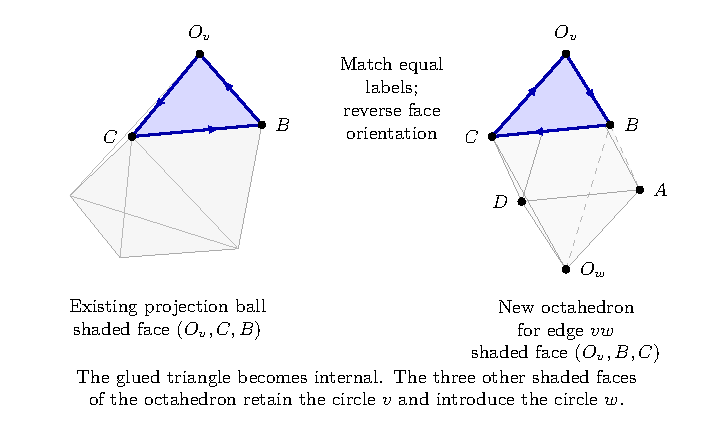
\includegraphics[width=.94\linewidth,keepaspectratio]{../book/figures/octahedral-page-attachment.pdf}
\caption{One ordered page attachment glues an edge block along a shaded triangle, retaining circle v and introducing circle w.}
\end{figure}

The attachment follows the original order of the tangle factors.
Its shaded triangle is glued to the designated disk page; the remaining
faces carry the new circle and the continuing main strands.

\subsection{Positive main meridians and their flags}\label{gi:positive-main-meridians-and-their-flags}

The bipartition signs describe native page coordinates. They are
not extra choices of the knot orientation. At a main boundary
vertex, take the actual small oriented meridian word supplied by
the physical collar. Its local derivative at the displayed ideal
point is \(m\) or \(m^{-1}\), depending on whether that native
meridian is the positive one or its inverse. Transport the word
and its eigenflag together through each face map.

For a main component, choose its orientation at one segment.
The same oriented small meridian propagates by the actual
annular collar conjugacies. The geometric ideal flag propagates
by those same conjugacies, so its chosen eigenvalue stays fixed.
There is no freedom to exchange it after returning around the
component: for generic \(M\), the peripheral longitude commutes
with a nonparabolic meridian and hence preserves both eigenlines.
At \(M=1\) use the analytic limit of this transported flag.
Thus one can record which global component orientation makes
the displayed flag the \(M^{-1}\) source flag. For a knot this
is one global orientation choice, not a separate reset at each
edge. A comparison with an already specified positive
meridian must make this initial choice explicitly.

This argument identifies the local auxiliary products for the
pure tree. Sections~\ref{gi:boundary-isotropy-and-the-edge-differential}--\ref{gi:determining-the-monomial-and-the-preferred-framing} identify the preferred main longitude
using the full boundary representation and its framing.

\subsection{Why the old odd three-point maps cannot be inserted unchanged}\label{gi:why-the-old-odd-three-point-maps-cannot-be-inserted-unchanged}

In the local chart keep the pure white maps \(W_j\) fixed.
Let \(A_{\mathrm o}\) and \(B_{\mathrm o}\) be the unique
three-point maps with the old odd permutations
\[
 (A,\infty,1)\mapsto(a,S,0),\qquad
 (A,R,0)\mapsto(a,\infty,1).
\]
They are

\begin{equation}\label{gi:S6}
A_{\mathrm o}=
 \begin{pmatrix}S&-S\\1&S(A-1)/a-A\end{pmatrix},\qquad
 B_{\mathrm o}=
 \begin{pmatrix}(a(A-R)+R)/A&-R\\1&-R\end{pmatrix}.
\end{equation}

The first original odd edge return is not trivial:

\begin{equation}\label{gi:S7}
W_0^{-1}B_{\mathrm o}W_2^{-1}A_{\mathrm o}:
             z\longmapsto m^{-2}z+(1-m^{-2})A.
\end{equation}

The second return is likewise nontrivial; the third,
\(W_1^{-1}B_{\mathrm o}W_3^{-1}A_{\mathrm o}\), is
projectively the identity. In particular the two defects vanish
at \(M=1\), which is why the old parabolic calculation did not
detect them.

Equation \eqref{gi:S7} is an obstruction to keeping both the pure white
charts and the old odd vertex assignment. It is not an
obstruction to the half-twist homeomorphism. That homeomorphism
must transport the puncture eigenflags and the adjacent charts.

\subsection{A regular matrix implementing the actual positive braid collar}\label{gi:a-regular-matrix-implementing-the-actual-positive-braid-collar}

Let \(a,b\in\mathrm{SL}_2(\mathbb C)\) be the two ordered
puncture meridians in the physical braid frame. They have the
same trace \(M+M^{-1}\). The original positive crossing
convention is

\begin{equation}\label{gi:S8}
(a,b)\longmapsto(a^{-1}ba,a),\qquad P=ba.
\end{equation}

This is the literal Wirtinger rule of
\href{https://sashakolpakov.github.io/murakamis_dream/notes/marked_braid_holonomy.html}{the marked braid calculation},
section 5. In particular the preserved product is \(ba\),
not \(ab\).

Put

\begin{equation}\label{gi:S9}
H=P^{-1}-I.
\end{equation}

Near the auxiliary complete lift \(P\), whose trace is \(-2\),
\(\det H=2-\operatorname{tr}P\) is near \(4\).
There is no singular diagonalizing frame.
The Cayley--Hamilton identities for \(a,b\), with their equal
traces, give

\begin{equation}\label{gi:S10}
(P-I)a=b(P-I),\qquad
 (P-I)^2=(\operatorname{tr}P-2)P.
\end{equation}

Consequently \(H\) is projectively \((P-I)^{-1}\), it
commutes with \(P\), and

\begin{equation}\label{gi:S11}
HaH^{-1}=a^{-1}ba,\qquad HbH^{-1}=a.
\end{equation}

This is the exact positive collar rule \eqref{gi:S8}. Its inverse realizes
the negative crossing.

Suppose the selected auxiliary flag has \(P\)-eigenvalue
\(-Q\). The eigenvalue ratio of \(H\) at that flag is

\begin{equation}\label{gi:S12}
\frac{-Q^{-1}-1}{-Q-1}=Q^{-1}.
\end{equation}

Thus composing a pure auxiliary meridian with \(H^\epsilon\)
changes its similarity by \(Q^{-\epsilon}\). It keeps the
disk longitude \(P\) and its chosen flag.

There is an independent matrix calibration against the original
geometric collar. In the local chart set

\begin{equation}\label{gi:S13}
P=m^{-1}W_2^{-1}W_0.
\end{equation}

This is the determinant-one disk word and has selected
eigenvalue \(-Q\). At \(m=1\), for all nearby \(E_0,Q\),
not just at the complete point,

\begin{equation}\label{gi:S14}
S_v^{-1}(P^{-1}-I)=W_0^{-1}B_{\mathrm o}
                        \quad\text{projectively}.
\end{equation}

The right side is the original physical positive-\(R\)
meridian, by section 6 of
\href{https://sashakolpakov.github.io/murakamis_dream/notes/actual_conway_general_mask_marked_filling.html}{the marked mask filling proof}.
Its inverse crossing is the other old odd path.
Equations \eqref{gi:S8} and \eqref{gi:S14} fix both the braid sign and the actual
copy/collar marking; the sign has not been chosen from a desired
source formula.

\subsection{The full ordered boundary groups in the actual edge chart}\label{gi:the-full-ordered-boundary-groups-in-the-actual-edge-chart}

Let \(N_j=W_{j-1}^{-1}W_j\), with indices modulo four.
Their determinant-one lifts, in the order of the original
equatorial boundary, are

\begin{equation}\label{gi:S14a}
A_g=M^{-3}N_3,\qquad B_g=MN_0,\qquad
 C_g=MN_1,\qquad D_g=MN_2,\qquad
                    A_gB_gC_gD_g=I.
\end{equation}

Each trace is \(M+M^{-1}\). These lifts follow from
\(\det W_0=L,\det W_1=L/m,\det W_2=L/m^2,\det W_3=Lm\).
They include the native loop directions, which need not all be
positive main meridians.

The pure edge returns give the following complete boundary
intertwinings:

\begin{equation}\label{gi:S14b}
\begin{array}{c|c|c|c|c}
 \text{circle}&(a,b)\text{ on the input side}
 &(a',b')\text{ on the output side}&C_0&P=ba=b'a'\\ \hline
 v&(B_g,A_g)&(C_g^{-1},D_g^{-1})&S_v^{-1}&A_gB_g\\
 w&(B_g^{-1},C_g^{-1})&(A_g,D_g)&S_w^{-1}&(B_gC_g)^{-1}.
\end{array}
\end{equation}

Here \(C_0aC_0^{-1}=a'\) and \(C_0bC_0^{-1}=b'\).
For example the first row is equivalent to

\begin{equation}\label{gi:S14c}
S_v C_g S_v^{-1}=B_g^{-1},\qquad
 S_v D_g S_v^{-1}=A_g^{-1}.
\end{equation}

The second is equivalently
\(S_w A_gS_w^{-1}=B_g^{-1}\) and
\(S_w D_gS_w^{-1}=C_g^{-1}\).
These are consequences of the full white/shaded returns;
they may also be checked by direct multiplication of the local
matrices. The product columns agree because
\(D_g^{-1}C_g^{-1}=A_gB_g\) and
\(D_gA_g=(B_gC_g)^{-1}\).

The disk convention \(P=ba\) is therefore explicit at both
ends, including the inversions caused by the turned second
circle. The same table transports under the actual conjugating
frames in a tree; an orientation reversal transports the whole
tuple and its disk word. It does not silently replace \(P\)
by a different boundary product.

For the positive braid put \(H=P^{-1}-I\) in the input
frame. Then \(C_+=C_0H\) satisfies

\begin{equation}\label{gi:S14d}
\begin{aligned}
 C_+aC_+^{-1}&=a'^{-1}b'a',\\
 C_+bC_+^{-1}&=a',\\
 C_+PC_+^{-1}&=P .
\end{aligned}
\end{equation}

For the negative braid use \(H^{-1}\) and the inverse
automorphism. Thus the construction checks both generators of
the actual twice-punctured disk and its outer boundary word;
it is stronger than checking a peripheral similarity or three
traces. Formula \eqref{gi:S14} fixes the positive crossing in the
original physical convention.

\subsection{The opposite-eigenflag qualification}\label{gi:the-opposite-eigenflag-qualification}

Let \(F_a,F_b\) be the two displayed puncture flags, with
eigenvalues \(\lambda_a,\lambda_b\). The natural braid output
flags for \eqref{gi:S8} are

\begin{equation}\label{gi:S15}
(a^{-1}F_b,F_a).
\end{equation}

Their eigenvalues are \((\lambda_b,\lambda_a)\), since
the strands have exchanged positions. By contrast,
\((HF_a,HF_b)\) has eigenvalues
\((\lambda_a,\lambda_b)\) on that same output tuple.
If the selected eigenvalues agree, the two descriptions coincide
by uniqueness of the relevant eigenline. If they differ, use
\(H\) on the opposite input eigenlines to obtain \eqref{gi:S15}.
At a native pure circle the geometric flags on its two main
punctures have opposite selections \(M^{-1},M\).
The qualification is therefore essential.

This identifies the error in an unqualified instruction to
transport both displayed flags by \(H\). The intertwiner is
correct; the displayed decorated triangle needs the accompanying
Weyl change. The two eigenlines coalesce at the parabolic point,
so the complete figure alone cannot distinguish the operations.

\subsection{Representation gluing followed by global decoration}\label{gi:representation-gluing-followed-by-global-decoration}

The following construction keeps that distinction explicit.
First perform the actual collar gluing at the level of
representations; then select the geometric eigenflags on the
resulting original link group.

The half-twist is the actual mapping cylinder of the two-punctured
disk, fixing its outer boundary. Its two boundary generator
tuples are related by \eqref{gi:S8}. If \(C\) is the pure boundary
intertwiner, replacing it by \(CH^\epsilon\), with the side
and composition order fixed by \eqref{gi:S14}, supplies the new
intertwiner. Equation \eqref{gi:S11} verifies the two puncture relations;
\([H,P]=0\) verifies the outer disk-boundary relation. These
are the generators and relation of the twice-punctured disk.
The van Kampen presentation of that actual cut therefore gives
the representation of the reglued exterior. It uses the one
distinguished disk seam at that circle, once.

Apply the operation in every original circle's transported
puncture frame. The other cyclic page seams remain those of
the pure-page construction above. At this stage no assertion is made that the old
pure ideal vertices still provide the correct decoration.

For each resulting main component, choose its actual positive
meridian and its \(M^{-1}\) eigenflag. At a corner whose
native loop is the inverse, take the corresponding \(M\)
eigenflag. Transport these choices by the original paths in the
completed cut. Peripheral commutation makes the choice independent
of a peripheral path. Keep the already selected disk-longitude
flag on each auxiliary circle.

These choices are holomorphic near the complete structure.
For example, for a noncentral matrix
\(\left(\begin{smallmatrix}a&b\\c&d\end{smallmatrix}\right)\)
with \(b\ne0\), an eigenline with prescribed holomorphic
eigenvalue \(\lambda\) is represented by
\((b,\lambda-a)\). The opposite eigenline is obtained by
replacing \(\lambda\) by \(\lambda^{-1}\).
Both approach the unique parabolic flag at the complete point.
A change of coordinate handles a chart with \(b=0\).
The same argument applies to the selected auxiliary eigenvalue
\(-Q\).

Develop the original topological ideal triangulation from these
global flags and the constructed representation. The map of
each triangle is the unique map of its transported ordered
triple. Adjacent white maps must be rebuilt in this way;
\eqref{gi:S7} shows why they cannot generally be retained unchanged.
Equivariance gives every edge return. At the complete parameter,
\eqref{gi:S14} and the original collar convention identify the actual odd
development. Its positively oriented tetrahedra therefore remain
positive in a sufficiently small neighborhood of the fixed
finite tree. This is a local decorated representation
construction, not a global completeness assertion for a
nonparabolic main cusp.

The tuple with \(P=ba\) is exactly \eqref{gi:S14b}, transported in the
original physical collar. The positive main loops are chosen
in the completed cut. For the canonical four-segment traversal,
they are \(C_g,B_g^{-1},A_g,D_g^{-1}\) at
\(\infty,0,R,1\), respectively; all four select their geometric
corner with eigenvalue \(M^{-1}\). A reversed physical route
transports both its loop direction and its flag. The preceding
opposite-eigenflag calculation describes the required Weyl change.

At representation level the primitive auxiliary increment is

\begin{equation}\label{gi:S16}
U_v^{\exp}
       =Q_v^{-\epsilon_v}
          \prod_{e\ni v}\frac{Q_v+X_e}{1+Q_vX_e},\qquad
 V_v^{\exp}=Q_v^2.
\end{equation}

It is unchanged by the main-flag redecoration. The exponentiated filling
equation with \(n_v=\epsilon_v-2p_v\) is then

\begin{equation}\label{gi:S17}
\prod_{e\ni v}\frac{Q_v+X_e}{1+Q_vX_e}
                                =Q_v^{n_v}.
\end{equation}

The auxiliary formulas retain the original circle words. The main
preferred longitude is determined in Sections~\ref{gi:boundary-isotropy-and-the-edge-differential}--\ref{gi:determining-the-monomial-and-the-preferred-framing} using boundary
isotropy, algebraic regularity and the independently marked cusp.
The argument does not replace a boundary word by a scalar simply
because the local representation has the correct traces.

\section{The complete anchor and the primitive filling equations}\label{gi:the-complete-anchor-and-the-primitive-filling-equations}

At \(M=1\), the local charts reduce to the
\href{https://sashakolpakov.github.io/murakamis_dream/notes/actual_all_circle_angular_octahedra.html}{angular octahedral charts}.
Their white/shaded words and primitive disk longitude agree with the
ones above. Their complete flags and oriented tetrahedral shapes
give the marked complete structure of the original augmented
exterior. The
\href{https://sashakolpakov.github.io/murakamis_dream/notes/general_marked_multicusp_gluing_rigidity.html}{multicusp gluing rigidity theorem}
identifies the nearby decorated representation with that marked
geometric germ; this uses the full original peripheral rows, not
only equality of their traces.

The pure meridian increments multiply around each circle in its
actual cyclic order. The one retained half twist contributes
\(Q_v^{-\epsilon_v}\), with the sign calibrated in \eqref{gi:S14}.
Thus, on the continued marking,

\begin{equation}\label{gi:A1}
U_v=\sum_{e\ni v}\log\rho_{v,e}-\epsilon_v\log Q_v,\qquad
 V_v=2\log Q_v.
\end{equation}

These are logarithms of the squared eigenvalues of the original
primitive auxiliary curves. No peripheral power is substituted.

For a branch supplied by the
\href{https://sashakolpakov.github.io/murakamis_dream/notes/actual_all_circle_geometric_completion.html}{geometric completion theorem}
or the corresponding marked long-filling theorem, the original
primitive logarithmic equation is

\begin{equation}\label{gi:A2}
U_v+p_vV_v=-2\pi i.
\end{equation}

Its continued mark selects the original first-charge geometric
branch. More explicitly, let \(\Psi(\tau)\) be the angular action
obtained after the original wire variables have been made stationary,
with \(Q_v=e^{i\tau_v}\). The marked circle calculation gives
\(U_v=-2\pi\Psi_{\tau_v}-i\epsilon_v\tau_v\).
The charge path is therefore exactly

\begin{equation}\label{gi:A2a}
\Psi_{\tau_v}+\frac{in_v\tau_v}{2\pi}-ic=0
 \quad\Longleftrightarrow\quad
 U_v+p_vV_v=-2\pi ic,\qquad 0\le c\le1.
\end{equation}

The logarithms are continued from the complete point at \(c=0\);
the constant \(-ic\) is part of the primitive mark.
Exponentiation at \(c=1\) gives \eqref{gi:T5}, since
\(n_v=\epsilon_v-2p_v\). The exponentiated equation alone
does not select the logarithmic branch or prove smooth completion.
At the selected filled point write \(Q_v=e^{i\tau_v}\).
The completion has \(\operatorname{Im}\tau_v<0\), hence
\(Q_v^2\ne1\). Its auxiliary longitude is therefore semisimple
with distinct eigenlines. The filling word commutes with that longitude;
equation \eqref{gi:T5} says that its eigenvalue ratio is one. A matrix commuting
with a matrix having distinct eigenlines is diagonal in that eigenbasis,
so ratio one makes it scalar. Thus the filling word is projectively
identity, and this conclusion persists on a sufficiently small
neighborhood of the selected filled point.

The marked charge path identifies the representation at \(M=1\),
not only its peripheral eigenvalues. It begins with the original
complete octahedral charts. Along the path the same labeled face maps,
primitive disk curves and source \(M^{-1}\) flag are retained.
The positive-cell completion identifies its endpoint with the
holonomy of the original complete filled knot. For the marked
long-filling branch the same identification follows from its original
Dehn-filling construction.

When the selected source critical point is nondegenerate, its
implicit branch gives holomorphic \(Q_v(M)\) and \(X_e(M)\) near
that endpoint, retaining \eqref{gi:A2}. The reconstructed matrices then give
a branch of representations of the original filled group by the
preceding semisimple argument. The geometric meridian coordinate
is a local parameter at complete knot holonomy, by the
\href{https://sashakolpakov.github.io/murakamis_dream/notes/actual_geometric_normal_period.html\#3-the-geometric-critical-scheme-is-smooth-with-two-framing-directions}{geometric knot-germ construction}
and its marked gluing input. The
\href{https://sashakolpakov.github.io/murakamis_dream/notes/general_marked_multicusp_gluing_rigidity.html}{multicusp version}
supplies the corresponding representation and decoration comparison
where a positive complete triangulation is specified.
Consequently this branch is the geometric meridian germ with the
declared eigenflag. This is the branch used when a source asymptotic
is later compared with the geometric longitude.

Every statement below about a filled geometric longitude retains
this original complete/filling anchor. An exponentiated slope equation
on a different algebraic branch is insufficient.

\section{Boundary isotropy and the edge differential}\label{gi:boundary-isotropy-and-the-edge-differential}

\subsection{The edge equation and a closed differential}\label{gi:the-edge-equation-and-a-closed-differential}

For an edge with endpoint variables \(Q,P\), let \(X\) satisfy

\begin{equation}\label{gi:R1}
(X+Q)(X+Q^{-1})(X+P)(X+P^{-1})
      =(X-1)^2(1-XM^2)(1-X/M^2).
\end{equation}

The variables are nonzero. We work first where all displayed factors
are nonzero and the selected root is simple. Write

\begin{equation}\label{gi:R2}
\begin{gathered}
 u=\log M,\quad q=\log Q,\quad p=\log P,\quad z=\log X,\\
 f=\frac{M^2-X}{1-M^2X},\quad
 \rho_Q=\frac{Q+X}{1+QX},\quad
 \rho_P=\frac{P+X}{1+PX}.
 \end{gathered}
\end{equation}

Only the differentials of the logarithms will be used. Their branches
therefore do not affect the identities below.

Let \(F\) be the logarithm of the quotient of the two sides of
\eqref{gi:R1}, holding \(z,q,p,u\) independent before differentiating.
Direct differentiation gives

\begin{equation}\label{gi:R3}
F_u=2(\log f)_z,\qquad
 F_q=-(\log\rho_Q)_z,\qquad
 F_p=-(\log\rho_P)_z.
\end{equation}

On the edge surface \(dF=0\). Moreover \(f\) has no direct
\(q,p\) dependence, and each \(\rho\) has no direct
\(u\) dependence or dependence on the other endpoint. Thus

\begin{equation}\label{gi:R4}
\begin{aligned}
 &du\wedge d\log f+
   \tfrac12d\log\rho_Q\wedge dq+
   \tfrac12d\log\rho_P\wedge dp\\
 &\quad=\tfrac12(F_u\,du+F_q\,dq+F_p\,dp)\wedge dz=0.
 \end{aligned}
\end{equation}

This proof uses the rational equation itself. It does not identify a
geometric volume by comparing numerical critical values. Since \eqref{gi:R4} is
an identity of rational differential forms, it holds on every smooth
part of the same algebraic component.

\subsection{The actual boundary pairing}\label{gi:the-actual-boundary-pairing}

Sections~\ref{gi:the-local-face-maps}--\ref{gi:ordered-pages-and-the-half-twist-collar} have assembled the ordered pieces into a representation
of the original augmented link exterior. Let \(L\) be the
eigenvalue of its preferred main longitude on the main
\(M\)-eigenline. At each auxiliary circle let \(U_v\) be the
logarithm of the primitive meridian similarity, and let the selected
longitude eigenvalue be \(-Q_v\). The exact local construction and
the original half-twist convention give

\begin{equation}\label{gi:R5}
U_v=\sum_{e\ni v}\log\rho_{v,e}-\epsilon_v\log Q_v,
 \qquad \epsilon_v\in\{-1,0,1\},
\end{equation}

up to locally constant logarithmic periods. The summands and the
primitive word must be established by the actual boundary gluing.

The infinitesimal boundary pairing is

\begin{equation}\label{gi:R6}
du\wedge d\log L+
             \tfrac12\sum_v dU_v\wedge d\log Q_v=0.
\end{equation}

Here all tori use the meridian--longitude orientations induced by the
same oriented exterior. The factor one half occurs because \(U_v\)
is a logarithm of an eigenvalue ratio, whereas \(\log Q_v\) is
a logarithm of a single determinant-one eigenvalue.

For completeness, \eqref{gi:R6} has a direct topological proof. Infinitesimal
variations of a representation are one-cocycles with values in its
adjoint local system. Pair two such cocycles by
\(\operatorname{tr}(XY)\) and take their cup product. The result
is a closed ordinary two-cochain, because the trace pairing is
invariant under conjugation. Its total evaluation on the boundary
of a fundamental three-chain is zero by the cochain Stokes identity.
On a torus with commuting diagonal holonomies, write their logarithms
as \(x\operatorname{diag}(1,-1)\) and
\(y\operatorname{diag}(1,-1)\). The alternating trace pairing
is \(2(dx\wedge dy)\). Summing over the boundary tori gives
\(\sum dx\wedge dy=0\). Substitute
\((x,y)=(u,\log L)\) at the main torus and
\((x,y)=(U_v/2,\log Q_v)\) at the auxiliary tori. This proves
\eqref{gi:R6} where the peripheral matrices are diagonalizable. The rational
identity extends over the remaining points where its terms are defined.

Subtract the sum of \eqref{gi:R4} over all edges from \eqref{gi:R6}. The half-twist term
in \eqref{gi:R5} has zero wedge product with \(d\log Q_v\). The result is

\begin{equation}\label{gi:R7}
du\wedge d\log\left(\frac{L}{\prod_e f_e}\right)=0.
\end{equation}

In particular, the discrepancy has no infinitesimal dependence on any
auxiliary variable. To avoid choosing determinant-one lifts globally,
use the squared discrepancy

\begin{equation}\label{gi:R8}
R=\frac{L^2}{\prod_e f_e^2}.
\end{equation}

It is a rational function whenever the original projective peripheral
representation is rational on the source variety: \(L^2\) is the
ratio of the two eigenvalues of the main longitude, with its ordered
main flag retained.

\section{The constant field of the source equations}\label{gi:the-constant-field-of-the-source-equations}

\subsection{Why the discrepancy is rational in the main meridian}\label{gi:why-the-discrepancy-is-rational-in-the-main-meridian}

Let \(k=\mathbb C(M)\), and let the graph have distinct unordered
edges. In particular this applies to a tree. The edge quadratic
gives, on putting \(Z=X+X^{-1}\):

\begin{equation}\label{gi:R9}
Z=\frac{2(M^2+M^{-2})-(Q+Q^{-1})(P+P^{-1})}
 {Q+Q^{-1}+P+P^{-1}+M^2+M^{-2}+2}.
\end{equation}

Work on the open set where these denominators are invertible; it
contains the complete branch. The squareclass of \(Z^2-4\) is

\begin{equation}\label{gi:R10}
H_e=(Q_v-1)^2(Q_w-1)^2
                  -4(M+M^{-1})^2Q_vQ_w.
\end{equation}

To see that the edge squareclasses are independent, extend the
coefficient field to an algebraic closure \(\overline{k}\).
Put \(t=(M+M^{-1})^2\ne0\) in this field. As a quadratic in
\(Y\), the polynomial
\((X-1)^2(Y-1)^2-4tXY\) has discriminant

\begin{equation}\label{gi:R11}
16tX[X^2+(t-2)X+1].
\end{equation}

Its order of vanishing at \(X=0\) is one, so it is not a square
in \(\overline{k}(X)\). Its coefficients in \(Y\) have no
common factor: at \(X=1\) the middle coefficient is \(-4t\).
It is therefore irreducible in \(\overline{k}[X,Y]\).

Different edges give different such prime polynomials, since they
involve different pairs of independent vertex variables. The valuation
at the prime \(H_e\) is odd for its own squareclass and zero for
every other edge. Hence every nonempty product of edge squareclasses
is nonsquare. Adjoining their square roots has degree \(2^{|\mathcal E|}\)
even after extending \(k\) to \(\overline{k}\). This proves
geometric integrality of the generic source fiber over \(M\).
In particular \(k\) is algebraically closed in its function
field \(\mathcal F\).

The logarithmic derivatives in all the \(Q_v\) extend uniquely
to the finite separable field \(\mathcal F\). If an element of
\(\mathcal F\) is killed by every such derivative, its relative
differential over \(k\) vanishes. In characteristic zero it is
algebraic over \(k\), and therefore belongs to \(k\) by the
preceding paragraph. Applying this to \eqref{gi:R7}--\eqref{gi:R8} gives

\begin{equation}\label{gi:R12}
R\in\mathbb C(M)^*.
\end{equation}

The specialization of \eqref{gi:R10} at \(M=\pm i\) is a square. This
does not invalidate the generic integrality proof; it does mean that
those fibers need the separate check in Section~\ref{gi:regular-reconstruction-at-every-nonzero-main-value}.

\section{Regular reconstruction at every nonzero main value}\label{gi:regular-reconstruction-at-every-nonzero-main-value}

\subsection{A uniform algebraic open set in every fiber}\label{gi:a-uniform-algebraic-open-set-in-every-fiber}

For one edge write

\begin{equation}\label{gi:G1}
m=M^2,\quad D=m+m^{-1},\quad
 \beta=Q+Q^{-1},\quad\gamma=P+P^{-1},\quad
 S=\beta+\gamma+D+2.
\end{equation}

Use \(X\) for the source wire coordinate. Its equation is the
quadratic

\begin{equation}\label{gi:G2}
F(X)=S(X^2+1)+(\beta\gamma-2D)X=0.
\end{equation}

This is equivalent, on \(X\ne0\), to the original degree-four
effective edge equation after its cancellation. Define

\begin{equation}\label{gi:G3}
J=\beta\gamma-2\beta-2\gamma-4D-4.
\end{equation}

The discriminant of \eqref{gi:G2} is

\begin{equation}\label{gi:G4}
\Delta=(\beta+2)(\gamma+2)J.
\end{equation}

Consider the open conditions

\begin{equation}\label{gi:G5}
\begin{gathered}
 QP\ne0,\qquad
 (\beta+2)(\gamma+2)(\beta+D)(\gamma+D)\ne0,\\
 S\ne0,\qquad \Delta\ne0.
\end{gathered}
\end{equation}

For every fixed \(M_0\in\mathbb C^*\), these conditions define
a nonempty Zariski open subset of the \(Q,P\) torus. Indeed each
excluded expression is a nonzero polynomial in the independent
variables \(\beta,\gamma\). For a fixed finite tree the same
conditions can be imposed simultaneously at every edge, since
their product is again a nonzero Laurent polynomial in the
vertex parameters \(Q_v\).

On \eqref{gi:G5}, both roots of \eqref{gi:G2} are finite, nonzero and distinct.
Several useful evaluations are

\begin{equation}\label{gi:G6}
\begin{aligned}
 F(1)&=(\beta+2)(\gamma+2),&
 F(-1)&=-J,\\
 F(m)&=m(\beta+D)(\gamma+D),&
 F(m^{-1})&=m^{-1}(\beta+D)(\gamma+D).
\end{aligned}
\end{equation}

Hence neither root is \(1,-1,m,m^{-1}\). In particular

\begin{equation}\label{gi:G7}
f=\frac{m-X}{1-mX}
\end{equation}

is a finite nonzero function at every point under consideration.
The auxiliary factors \((Q+X)/(1+QX)\) and
\((P+X)/(1+PX)\) are also finite and nonzero. To see this,
substitute \(X=-Q\) or \(X=-Q^{-1}\) in the original edge
equation. A zero can occur only when \(Q=-1\) or
\(Q=-m^{\pm1}\), excluded by \eqref{gi:G5}; the other endpoint is
identical.

\subsection{The actual character matrices remain regular}\label{gi:the-actual-character-matrices-remain-regular}

Put \(t=M+M^{-1}\), \(p=-\beta\), \(q=-\gamma\), and
\(\mathcal X=2+SX\). The character adapter uses

\begin{equation}\label{gi:G8}
A=\begin{pmatrix}M&1\\0&M^{-1}\end{pmatrix},\qquad
 B=\begin{pmatrix}M^{-1}&0\\p-2&M\end{pmatrix}.
\end{equation}

Its matrix \(C\) is given by

\begin{equation}\label{gi:G9}
\begin{gathered}
 h=M-M^{-1},\qquad
 c=\frac{M\mathcal X+M^{-1}q-2t}{D-p},\\
 d=\frac{q-M^2-1+hc}{p-2},\qquad
 e=\mathcal X-1-M^{-2}-hc,\qquad
 C=\begin{pmatrix}c&d\\e&t-c\end{pmatrix},\\
                         D_0=(ABC)^{-1}.
\end{gathered}
\end{equation}

The only denominators in \eqref{gi:G8}--\eqref{gi:G9}, besides powers of \(M\),
are \(p-2=-(\beta+2)\) and \(D-p=D+\beta\).
They are units on \eqref{gi:G5}. The four matrices have determinant one
and trace \(t\), with
\(\operatorname{tr}(AB)=-\beta\) and
\(\operatorname{tr}(BC)=-\gamma\), by \eqref{gi:G2}.
The formulas contain no division by \(M-M^{-1}\) or by \(t\).

The pure auxiliary transports are

\begin{equation}\label{gi:G10}
V=AB-\frac{1+X(\beta+1)}{1-X}I,\qquad
 T=BC+\frac{X+\gamma+1}{1-X}I.
\end{equation}

They satisfy the full puncture conjugacies, not just the trace
equations. Their determinants simplify on \eqref{gi:G2} to

\begin{equation}\label{gi:G11}
\det V=\frac{X(\beta+2)^2(\beta+D)}{S(X-1)^2},\qquad
 \det T=\frac{X(\gamma+2)^2(\gamma+D)}{S(X-1)^2}.
\end{equation}

For example the first determinant before reduction is
\[
 \frac{(\beta+2)(X^2+\beta X+1)}{(X-1)^2}.
\]
Equation \eqref{gi:G2} implies
\(X+X^{-1}+\beta=(\beta+2)(\beta+D)/S\), giving \eqref{gi:G11}.
The second computation is the same with \(\gamma\).
Thus both full transport matrices and their inverses are regular
on \eqref{gi:G5}, on either root of the source equation.

Every disk boundary pair is irreducible there. For the first
pair the standard direct trace calculation gives

\begin{equation}\label{gi:G12}
\operatorname{tr}[A,B]-2=(\beta+2)(\beta+D)\ne0.
\end{equation}

The second has the corresponding \(\gamma\) formula.
One can also derive \eqref{gi:G12} directly from the two matrices \eqref{gi:G8}.
For determinant-one two-generator representations this
nonzero expression excludes a common invariant line. In
particular neither generator is central.

The positive odd collar uses \(H=P_{\mathrm{disk}}^{-1}-I\)
with the original ordered disk product. Since
\(\operatorname{tr}P_{\mathrm{disk}}=-\beta\),

\begin{equation}\label{gi:G13}
\det H=2+\beta\ne0.
\end{equation}

The same holds at the other endpoint. The actual positive and
negative Hurwitz generators and all fixed powers remain
invertible. Thus odd seams introduce no exceptional fixed
value of \(M\).

\subsection{Sewing finitely many blocks uses a rational finite atlas}\label{gi:sewing-finitely-many-blocks-uses-a-rational-finite-atlas}

The ordered page construction glues two boundary pairs whose
matrices are explicit rational functions of the edge variables.
Their identification is the actual one in the native table;
where a loop is inverted or its order reversed, that operation
is included before asking for an intertwiner.

After those marked identifications, the two ordered boundary
pairs have the same three traces and are irreducible by \eqref{gi:G12}.
Their intertwiner is the solution line of

\begin{equation}\label{gi:G14}
G a=a'G,\qquad G b=b'G.
\end{equation}

The solution line is one-dimensional, and every nonzero solution
is invertible. Indeed a nontrivial kernel or image would be an
invariant line for one of the two irreducible pairs. Existence
can be proved without using ideal vertices. For an irreducible
pair the four matrices \(I,a,b,ab\) span
\(\operatorname{Mat}_2\). Their multiplication table is
determined by the common trace \(t\) and product trace \(p\):

\begin{equation}\label{gi:G14a}
a^2=ta-I,\quad b^2=tb-I,\quad
 ab+ba=t(a+b)+(p-t^2)I.
\end{equation}

The same table for the primed pair gives an isomorphism of
the two full matrix algebras, hence conjugation by an
invertible matrix. Equivalently put both pairs in the
explicit form \eqref{gi:G8}; irreducibility ensures that the two
selected generator flags are distinct and that the
off-diagonal entry used to normalize the frame is nonzero.
Either proof retains the ordered generators, not just the
individual conjugacy classes.

Equation \eqref{gi:G14} is a finite linear system with rational entries.
Choose a nonzero maximal minor and normalize one coordinate
on its one-dimensional kernel. This gives a rational
intertwiner regular in a neighborhood of that point.
No single choice of minor has to work at all parameters.
The finitely many choices form a rational atlas; the resulting
representation and peripheral eigenvalue ratios are independent
of the scalar normalization of an intertwiner.

Start with one edge block. The actual page insertion joins each
new block to the preceding union along one marked disk side.
Its attaching graph is a tree of blocks, so this inductively
constructs a representation of the entire page-cut object with
all matrices regular. The distinguished pure or odd seam at
each circle is then installed using \eqref{gi:G10}, \eqref{gi:G13}, and the two
full generator conjugacies of its actual mapping cylinder.
Those formulas preserve its outer disk product. Van Kampen
therefore gives the representation of the original augmented
exterior. No arbitrary pants permutation or commutativity of
tangles is used.

For any fixed finite tree, intersecting the finitely many
necessary open charts gives a nonempty open set over the
fixed \(M_0\). Equivalently, at any good point one may choose
each nonzero intertwiner minor in succession, obtaining a
regular neighborhood of that point. This proves existence of
the required actual rational \(\mathrm{PGL}_2\) reconstruction
at every nonzero main parameter.

This step requires the actual marked boundary conjugacies,
not just a formal family of characters. They were identified
with the original cut in the page/collar proof and remain
rational identities on the present open sets.

\subsection{The exceptional-looking main parameters}\label{gi:the-exceptional-looking-main-parameters}

At \(M=\pm1\), one has \(D=2\). Conditions \eqref{gi:G5} simply
exclude \(\beta=-2,\gamma=-2\), together with the stated
nonzero discriminant and denominator. The main matrix in
\eqref{gi:G8} is a noncentral parabolic. Nothing in \eqref{gi:G8}--\eqref{gi:G14} divides
by its eigenvalue difference, so the reconstruction is regular.

At \(M=\pm i\), one has \(D=-2\). The source discriminant
becomes

\begin{equation}\label{gi:G15}
\Delta=(\beta^2-4)(\gamma^2-4).
\end{equation}

With \(\beta=Q+Q^{-1}\) and \(\gamma=P+P^{-1}\),
this is a square in \(\mathbb C(Q,P)\). The fiber therefore
splits; generic-fiber irreducibility must not be asserted
at these two values. Nevertheless \eqref{gi:G5} gives two distinct
simple roots at generic \(Q,P\), and all matrices \eqref{gi:G8}--\eqref{gi:G14}
are regular. The main punctures are semisimple, with
eigenvalues \(i,-i\) or \(-i,i\), and remain noncentral.
The two roots can be written explicitly as

\begin{equation}\label{gi:G15a}
X=-\frac{Q+P}{1+QP},\qquad
             X=-\frac{1+QP}{Q+P}.
\end{equation}

For generic \(Q,P\) they differ and avoid \(1,-1\).
Fixing these auxiliary values, the implicit-function theorem
for \eqref{gi:G2} therefore continues either root holomorphically in
\(M\) through \(M_0=i\) or \(-i\).

The native ideal cell chart explains a possible false alarm.
At \(m=-1\), its preliminary white coordinate \(E_0\)
satisfies

\begin{equation}\label{gi:G16}
(E_0P-E_0Q-PQ+1)(E_0PQ-E_0-P+Q)=0.
\end{equation}

On one branch the two minus-copy circle apices coincide; on
the other the plus-copy apices coincide. Thus that particular
eight-tetrahedron ideal subdivision degenerates. This does
not make the actual group matrices singular: \eqref{gi:G8}--\eqref{gi:G14} are
an explicit regular reconstruction at precisely those points.
The rigidity argument needs the latter, not a positive
triangulation at every complex value of \(M\).

\subsection{A regular nonzero main eigenvalue ratio}\label{gi:a-regular-nonzero-main-eigenvalue-ratio}

Every main peripheral word is a fixed finite product of the
regular invertible group matrices just constructed. Hence its
matrix and inverse are regular at the chosen point.
The main meridian is noncentral.

There is one important trace-zero detail. Commutation in
\(\mathrm{PGL}_2\) alone would allow a longitude to
exchange the two eigenlines of a trace-zero meridian.
Use the matrices on the local section through nearby \(M\).
Normalize the meridian \(\mu\) to determinant one.
Its projective commutation with a regular invertible
longitude representative \(L\) gives
\(L\mu L^{-1}=\kappa\mu\), where
\(\kappa^2=1\) by determinants. At the nearby parameters
with \(M+M^{-1}\ne0\), taking traces gives \(\kappa=1\).
Consequently the exact matrix identity

\begin{equation}\label{gi:G16a}
L\mu=\mu L.
\end{equation}

extends to the trace-zero point. The undesired
anticommuting component is not part of this continued
representation. This also follows as a rational identity
on the integral generic source family.

At \(M_0\ne\pm1\), choose
its specified eigenline locally; its eigenvalue on a commuting
peripheral word is finite and nonzero. The ratio of the two
peripheral eigenvalues is therefore a regular unit.

The same conclusion holds at \(M_0=\pm1\), without
diagonalizing the meridian. In a frame in which its
upper-right entry is a unit, a commuting matrix \(L\) has
the form

\begin{equation}\label{gi:G17}
L=aI+b\mu.
\end{equation}

Here \(b=L_{12}/\mu_{12}\) and
\(a=L_{11}-b\mu_{11}\) are regular. Its two selected
eigenvalues are \(a+bM\) and \(a+bM^{-1}\). Both are
nonzero at the point because \(\det L\ne0\).
Their ratio is therefore regular and nonzero through the
parabolic value. Scalar changes of the representative \(L\)
cancel from the ratio.

The selected meridian eigenline itself is regular as well:
in this frame it is spanned by
\((\mu_{12},M-\mu_{11})\), or by
\((\mu_{12},M^{-1}-\mu_{11})\) for the other selection.
The first coordinate is a unit, including at \(M=\pm1\).
Thus coalescence of the two flags does not create a pole in
the marked eigenvalue ratio.

This directly applies to the square of a determinant-one
preferred-longitude eigenvalue, with the chosen inverse
convention if necessary. It does not require choosing a
global square root of a projective matrix determinant.
Every factor \eqref{gi:G7}, and every framing monomial in \(M\),
is likewise a unit at the point.

\subsection{Local sections and the integral total family}\label{gi:local-sections-and-the-integral-total-family}

More concretely, fix generic numerical auxiliary values
\(Q_v=q_v\) satisfying all the open conditions at \(M_0\),
and choose a simple root of every edge equation. The implicit
function theorem gives simultaneous holomorphic roots
\(X_e(M)\) near \(M_0\). At the chosen point select a
nonzero minor in each linear gluing system \eqref{gi:G14}. Those same
minors remain nonzero nearby. All actual group matrices,
their inverses and the main eigenvalue ratio are then
holomorphic along this local section. This is stronger than
the existence of an isolated good point in a special fiber.

The split trace-zero fibers do not invalidate this argument.
Let \(B\) be the Laurent coordinate ring in \(M,Q_v\),
localized at all \(S_e\). Dividing \eqref{gi:G2} by \(S_e\) makes
every edge polynomial monic with constant term one. The
simultaneous source algebra is therefore free over \(B\),
with basis the products \(\prod_e X_e^{\epsilon_e}\),
\(\epsilon_e\in\{0,1\}\). The independent generic edge
squareclasses imply that its generic localization is a
single field of degree \(2^{|\mathcal E|}\). Freeness embeds the
source algebra into that field; in particular the total
source variety is integral and has no additional vertical
component. Its simple points at \(M=\pm i\) belong to
the closure of the same generic family. A rational identity
proved there therefore holds on the regular local section
just constructed.

\section{Determining the monomial and the preferred framing}\label{gi:determining-the-monomial-and-the-preferred-framing}

By Section~\ref{gi:the-constant-field-of-the-source-equations} the discrepancy is a rational function of \(M\).
By Section~\ref{gi:regular-reconstruction-at-every-nonzero-main-value} its pullback is a regular unit along a local section
through every \(M_0\ne0\). If it had a zero or pole at \(M_0\),
that nonzero order would persist on the section. Therefore it has
no zero or pole on \(\mathbb C^*\), and

\begin{equation}\label{gi:F1}
\frac{L_{\mathrm{aug}}^2}{\prod_e f_e^2}=cM^k,\qquad
                  c\ne0,\quad k\in\mathbb Z.
\end{equation}

This is the elementary classification of units of
\(\mathbb C[M,M^{-1}]\). At the complete main cusp every
\(f_e=1\) and \(L_{\mathrm{aug}}^2=1\), so \(c=1\).

The \href{https://sashakolpakov.github.io/murakamis_dream/notes/actual_all_circle_preferred_cusp.html}{preferred-cusp calculation}
is a marked face-word calculation on the same original exterior:

\begin{equation}\label{gi:F2}
\tau_{\mathrm{main}}
      =a_{\mathrm{aug}}+2i\sum_e\cot(\pi x_e),\qquad
 X_e=e^{2\pi ix_e},\qquad
 a_{\mathrm{aug}}=-w_\epsilon-\sum_v\epsilon_v.
\end{equation}

The integer includes the retained half twists and the preferred
zero-linking correction. It is not inferred from \eqref{gi:F1}.

For completeness, the cusp shape equals the logarithmic slope
of this geometric eigenvalue curve. Near a noncentral parabolic
meridian write a commuting determinant-one longitude as
\(aI+b\mu\). Its eigenvalues are \(a+bM^{\pm1}\).
At \(M=1\), its projective translation divided by the
meridian translation is \(b/(a+b)\). Differentiating the
determinant-one relation shows that
\(d\log L/d\log M\) has the same value. Thus \eqref{gi:F2}
computes this derivative with the specified marking.

Since \(f_e(1,X)=1\) for every \(X\), its first
derivative receives no contribution from the derivative
of the wire:

\begin{equation}\label{gi:F3}
\left.\frac{d\log f_e}{d\log M}\right|_{M=1}
       =2\frac{1+X_e}{1-X_e}
       =2i\cot(\pi x_e).
\end{equation}

Equations \eqref{gi:F1}--\eqref{gi:F3} give \(k=2a_{\mathrm{aug}}\), proving
\eqref{gi:T4}. Tangent agreement fixes the exponent only after the
preceding argument has excluded every other rational factor.

Now let \(\ell_v=\operatorname{lk}(K,C_v)\).
The crossing disk has exactly two main punctures, so
\(\ell_v=0\) for opposite local strand directions and
\(\ell_v=\pm2\) for parallel directions. In the augmented
exterior,

\begin{equation}\label{gi:F4}
[\lambda_{\mathrm{aug}}]=\sum_v\ell_v[\mu_v],
             \qquad [\lambda_v]=\ell_v[\mu_K].
\end{equation}

After filling \(\mu_v+p_v\lambda_v\), its meridian has
class \(-p_v\ell_v[\mu_K]\). The original main-boundary
word that becomes the preferred filled longitude is therefore

\begin{equation}\label{gi:F5}
\lambda_{\mathrm{fill}}
       =\lambda_{\mathrm{aug}}\,
                       \mu_K^{\sum_vp_v\ell_v^2}.
\end{equation}

This is a primitive integral basis change on the same main
torus. It is not an assertion that the augmented longitude
was already zero linking after surgery.

\begin{figure}
\centering
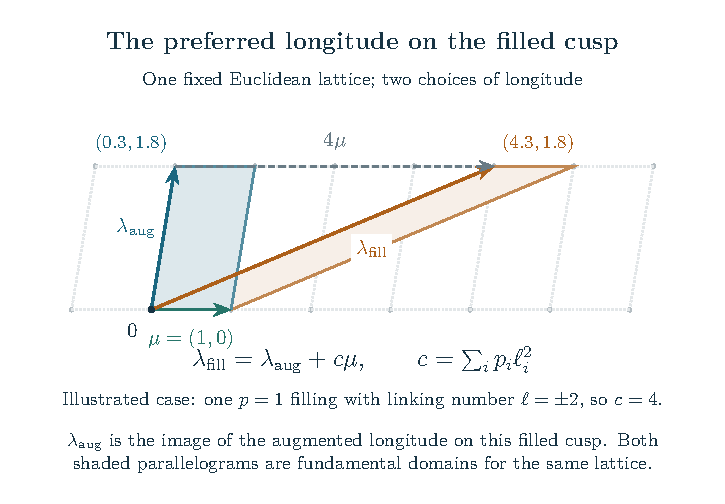
\includegraphics[width=.94\linewidth,keepaspectratio]{../book/figures/main-cusp-longitude-shear.pdf}
\caption{The image of the augmented longitude and the preferred filled longitude differ by an integral meridian shear on the same filled cusp.}
\end{figure}

Here \(\lambda_{\mathrm{aug}}\) means its image on the filled
cusp. Both shaded parallelograms use the same meridian and the
same lattice; the displayed example has
\(\sum_vp_v\ell_v^2=4\).

Write \(o_v=1\) for parallel and \(o_v=-1\) for
opposite strand directions in the fixed physical convention.
Then
\[
 \ell_v^2=2(1+o_v),\qquad
 w_\epsilon=\sum_vo_v\epsilon_v,\qquad
 w(D)=w_\epsilon-2\sum_vo_vp_v.
\]
Consequently

\begin{equation}\label{gi:F6}
\begin{aligned}
 a_{\mathrm{aug}}+\sum_vp_v\ell_v^2
  &=-w_\epsilon-\sum_v\epsilon_v+2\sum_vp_v(1+o_v)\\
  &=-w(D)-\sum_v(\epsilon_v-2p_v)=a(D).
\end{aligned}
\end{equation}

Combining \eqref{gi:T4} with \eqref{gi:F5}--\eqref{gi:F6} proves the squared filled
identity \eqref{gi:T6}, with the original primitive slopes and
preferred longitude.

\section{The determinant-one sign at the complete filled knot}\label{gi:the-determinant-one-sign-at-the-complete-filled-knot}

The squared identity leaves a two-valued ambiguity. Its sign is
fixed at the actual complete filled knot, rather than chosen
to fit the edge product.

The negative trace of a null-homologous peripheral curve is a known
fact; see Menal-Ferrer and Porti,
\cite[Corollary 3.10]{MenalFerrerPorti2012}.
The frame proof below includes the sign and its compatibility with
the lifts used here.

\subsection{A frame calculation on a once-bordered surface}\label{gi:a-frame-calculation-on-a-once-bordered-surface}

Let \(S\) be a compact connected oriented surface of genus \(g\)
with one boundary component. Embed it in an oriented three-manifold
which has a spin structure. Choose a smooth oriented tangent frame
\((e_1,e_2)\) on \(S\), and complete it by the positive unit normal
\(\nu\). Such a tangent frame exists because a surface with
boundary has trivial tangent bundle.

Pulling back the ambient spin double cover along
\((e_1,e_2,\nu)\) gives a double cover of \(S\).
Its monodromy is a homomorphism
\(H_1(S;\mathbb Z/2)\to\mathbb Z/2\).
Since the single oriented boundary is zero in this homology,
the lift of this chosen frame closes after one boundary circuit.

Now replace the first tangent vector on the boundary by its positive
unit tangent \(t\), and the second by the corresponding inward
tangent normal \(n\). Relative to \((e_1,e_2)\), the
frame \((t,n)\) has winding number

\begin{equation}\label{gi:L1}
\chi(S)=1-2g.
\end{equation}

This is the boundary form of the index formula: extend the outward
boundary normal to a tangent vector field with isolated zeros.
The sum of its indices is \(\chi(S)\); measured in the
global tangent frame, it is the degree of its boundary direction.
The boundary tangent differs from that normal by a fixed quarter
turn, which does not change the degree.

A full \(2\pi\) rotation in the tangent plane is the nontrivial
loop of the oriented three-dimensional frame group. It therefore
changes the sign of a spin lift. Formula \eqref{gi:L1} is odd. It follows
that the boundary-adapted frame

\begin{equation}\label{gi:L2}
(t,n,\nu)
\end{equation}

has an antiperiodic lift: after one boundary circuit its lift
returns to the other sheet.

No choice of spin structure changes this conclusion. The only
possible change was the monodromy of the first global frame,
and that monodromy vanishes on the boundary.

\subsection{Application to a complete hyperbolic knot cusp}\label{gi:application-to-a-complete-hyperbolic-knot-cusp}

Let \(Y\) be the oriented complete finite-volume hyperbolic complement
of a knot in \(S^3\). Take a sufficiently far cusp torus \(T\).
Its preferred longitude \(\lambda\) is primitive and bounds
a Seifert surface in the truncated complement.
Arrange the boundary of the surface to be the straight Euclidean
representative of \(\lambda\) on \(T\), and arrange its
collar to meet \(T\) orthogonally. These changes are made
inside the ordinary product collar of the boundary torus.

Along that boundary, \eqref{gi:L2} is a translation-invariant horospherical frame, up to
one constant rotation: \(t\) is the constant longitude
direction, \(n\) is the radial direction, and \(\nu\)
is the constant perpendicular direction in the horosphere.
Thus the preceding surface calculation says that the translation-invariant horospherical frame has
antiperiodic spin holonomy along \(\lambda\).

For precision, identify the oriented frame bundle of hyperbolic
three-space with \(\mathrm{PSL}_2(\mathbb C)\), and its
spin cover with \(\mathrm{SL}_2(\mathbb C)\).
Conjugate the cusp fixed point to infinity. If the longitude
translation is \(z_\lambda\ne0\), the path of translation-invariant
horospherical frames is represented by

\begin{equation}\label{gi:L3}
U(t)=
 \begin{pmatrix}1&t z_\lambda\\0&1\end{pmatrix},
                         \qquad 0\le t\le1.
\end{equation}

This is the lift starting at the identity.
Here translation-invariant refers to the cusp's Euclidean translation
group; no assertion of Levi-Civita parallel transport along a
horocycle in hyperbolic three-space is needed.
For a determinant-one holonomy lift \(\widetilde\rho\),
the endpoint of \eqref{gi:L3} closes in the quotient spin bundle precisely
when
\(\widetilde\rho(\lambda)=U(1)\).
It returns to the opposite sheet precisely when
\(\widetilde\rho(\lambda)=-U(1)\).
The antiperiodicity just proved therefore gives

\begin{equation}\label{gi:L4}
\boxed{\displaystyle
 \widetilde\rho(\lambda)=
       -\begin{pmatrix}1&z_\lambda\\0&1\end{pmatrix},
 \qquad
 \operatorname{tr}\widetilde\rho(\lambda)=-2.}
\end{equation}

Reversing the longitude replaces this matrix by its inverse and
does not change the sign. Any two determinant-one lifts differ
by a character to \(\{\pm1\}\), and the preferred longitude
is zero in the knot complement's first homology, so \eqref{gi:L4} is
independent of that choice as well.

Here spin existence needs no general three-manifold theorem.
Remove a point of the knot from \(S^3\); its complement is
\(\mathbb R^3\), whose standard tangent frame restricts to \(Y\).
Orthonormalizing for the hyperbolic metric gives a spin structure
on its oriented frame bundle and hence a lift of its geometric
holonomy. The sign calculation itself is the explicit surface-frame
argument above.

\subsection{Compatibility with the original augmented representation}\label{gi:compatibility-with-the-original-augmented-representation}

Return to the original all-circle construction. Write
\(\mu_K\) for its main meridian and \(\mu_v\) for its
original auxiliary meridians. The original circles are pairwise
unlinked. If \(\ell_v\) is the linking number of circle
\(v\) with the main knot and \(p_v\) is its integral
filling coefficient, the fixed main-boundary word which becomes
the preferred filled longitude is

\begin{equation}\label{gi:L5}
\lambda_{\mathrm{fill}}
       =\lambda_K\mu_K^{\sum_vp_v\ell_v^2}.
\end{equation}

In the augmented exterior its first homology class is

\begin{equation}\label{gi:L6}
[\lambda_{\mathrm{fill}}]
      =\sum_v\ell_v[\mu_v]
           +\sum_vp_v\ell_v^2[\mu_K].
\end{equation}

The original crossing disk is punctured by exactly two main
strands, so

\begin{equation}\label{gi:L7}
\ell_v\in\{0,2,-2\}.
\end{equation}

Consequently \eqref{gi:L6} vanishes modulo two.

At an actual complete filled knot point, pull back any
determinant-one lift of its complete holonomy to the augmented
group. Locally this lift continues through the augmented geometric
family: lift the finitely many generator matrices holomorphically;
the signs of the finitely many relations are discrete and remain
their identity values at the initial point.
If another local determinant-one lift is used for the face
construction, its ratio with this lift is a
\(\{\pm1\}\)-valued character: both project to the same
projective representation after one fixed conjugation.
By \eqref{gi:L6}--\eqref{gi:L7}, that character is one on
\(\lambda_{\mathrm{fill}}\).
Thus any such local face-map lift has exactly the same longitude
sign as the filled lift in \eqref{gi:L4}. A globally rational
determinant-one lift over the entire source variety is not
assumed or needed.

This step is useful because the original matrices of an auxiliary
filling slope may be \(-I\) rather than \(I\). One need not
assume that the particular auxiliary lifts descend to the filled
group. Their possible discrepancy is a character and cannot
change \eqref{gi:L5}.

\subsection{Fixing a holomorphic squared longitude identity}\label{gi:fixing-a-holomorphic-squared-longitude-identity}

The squared identity proved above, on a connected geometric germ
with the original selected main flag and fixed filling equations, is

\begin{equation}\label{gi:L8}
L_{\mathrm{geom}}^2
     =M^{2a(D)}
          \prod_e\left(\frac{M^2-X_e}{1-M^2X_e}\right)^2.
\end{equation}

The factors are holomorphic units near its complete filled point. Define
the longitude coordinate as the inverse eigenvalue on the source
\(M^{-1}\) meridian line. The ratio of the two sides before
squaring is then a holomorphic function taking values in
\(\{1,-1\}\); it is constant on the connected germ.

At the actual complete filled point, \(M=1\).
Each edge factor in \eqref{gi:L8} is one, since the geometric wire does
not have \(X_e=1\). The inverse selected longitude eigenvalue
is \(-1\) by the preceding complete-cusp and lift comparison. Therefore the constant is negative:

\begin{equation}\label{gi:L9}
\boxed{\displaystyle
 L_{\mathrm{geom}}
       =-M^{a(D)}
          \prod_e\frac{M^2-X_e}{1-M^2X_e}.}
\end{equation}

The conclusion requires the exact squared identity as input.
The complete-value sign fixes only its remaining two-valued
ambiguity; it is not being used to infer the dependence on \(M\)
or on any auxiliary parameter.

\section{The geometric factor of an actual quantum recurrence}\label{gi:the-geometric-factor-of-an-actual-quantum-recurrence}

The geometric identity now applies to the classical characteristic
selected by the actual invariant. This step uses the separate
\href{https://sashakolpakov.github.io/murakamis_dream/notes/actual_main_meridian_filtered_characteristic.html}{all-order source theorem};
the geometric construction by itself does not imply a quantum
asymptotic estimate.

\subsection{The source hypotheses and the factor statement}\label{gi:the-source-hypotheses-and-the-factor-statement}

Keep the original all-circle tree and knot qualifications of Section~\ref{gi:the-diagram-and-the-longitude-identity}.
Fix the signed powers and the diagram before the level tends to
infinity, and assume one of the following proved source hypotheses:

\begin{itemize}

\item
  the original strict presentation has independently sufficiently long
  fixed signed filling powers, as in the
  \href{https://sashakolpakov.github.io/murakamis_dream/notes/actual_main_meridian_filled_volume.html}{filled-meridian theorem};
\item
  its degrees and powers satisfy the
  \href{https://sashakolpakov.github.io/murakamis_dream/notes/actual_all_circle_quantitative_volume.html}{summed criterion},
  \(\sum_v d_v/(d_v^2+n_v^2)\le2^{-25}\);
\item
  they satisfy the
  \href{https://sashakolpakov.github.io/murakamis_dream/notes/actual_all_circle_local_message_volume.html}{local criterion},
  \(\max_v d_v/(d_v^2+n_v^2)\le2^{-120}\).
\end{itemize}

Here \(d_v\) is the number of edges incident to vertex \(v\).
The last two alternatives do not require every \(n_v\ne0\).
All original knot-pattern qualifications remain; in particular the
two-circle knot case excludes the two-odd link pattern. Both level
parities are retained.

Let \(F_N(M)\) be the actual zero-framed reduced ADO state, with

\begin{equation}\label{gi:O1}
q_N=e^{\pi i/N},\qquad M=-q_Nx,\qquad F_N(1)=K_N.
\end{equation}

The letter \(x\) here is the raw highest-weight parameter, not the
normalized internal index \(x_e\) with \(X_e=e^{2\pi ix_e}\).
Thus the marked complete meridian is \(M=1\). The
\href{https://sashakolpakov.github.io/murakamis_dream/notes/kashaev_ado_pointing.html}{ADO normalization and pointing} fix the
state and its complete value \(K_N\).

Consider any specified nonzero fixed operator

\begin{equation}\label{gi:O2}
P(q,M,T)=\sum_{j=0}^{d}a_j(q,M)T^j,\qquad
 a_j\in\mathbb C(q,M),\qquad TM=qMT,
\end{equation}

which annihilates the whole function \(F_N(M)\) at every sufficiently
large level \(q=q_N\). The shift \(T\) replaces \(M\) by \(qM\).
This is an actual all-level annihilator. Its existence is proved
independently by the
\href{https://sashakolpakov.github.io/murakamis_dream/notes/finite_sum_annihilator.html}{finite-sum annihilator theorem};
it is not defined by fitting complete values or by adding a desired
geometric factor.

Clear its fixed rational denominators to obtain Laurent-polynomial
coefficients, and remove their common \(q-1\) valuation. Let
\(P_0(M,L)\ne0\) be the first classical symbol that remains. If the
original operator has negative shift powers, first multiply by a
power of \(T\); this contributes only a Laurent unit to its
classical symbol.

Let \(A_{\mathrm{geom},\mathbb C}(M,L)\) generate the Laurent
prime of the actual oriented geometric eigenvalue germ through
\((M,L)=(1,-1)\). The longitude is the preferred one in \eqref{gi:T7},
on the \(M\) line, equivalently the inverse eigenvalue on the
source \(M^{-1}\) line.

\textbf{Corollary.} Under the stated all-circle source hypotheses,

\begin{equation}\label{gi:O3}
A_{\mathrm{geom},\mathbb C}(M,L)\mid P_0(M,L)
       \quad\text{in }\mathbb C[M^{\pm1},L^{\pm1}].
\end{equation}

This is the selected irreducible geometric factor, defined up to a
nonzero Laurent monomial. It is not a claim about its multiplicity,
the other factors of the symbol, or the full classical A-polynomial.
The rational-coefficient version is stated in Section~\ref{gi:the-irreducible-factor-and-its-field-of-definition}.

\subsection{The exact reduced/full conversion}\label{gi:the-exact-reducedfull-conversion}

The normalization factors must be retained before taking the
classical symbol. Write

\begin{equation}\label{gi:O4}
H_N(s)=\frac{\sin\pi s}{N\sin(\pi s/N)},\qquad
 d_N(M)=\eta_N\frac{M-M^{-1}}{M^N-M^{-N}},\qquad
 d_N(1)=\frac{\eta_N}{N},\quad \eta_N=i^{N+3}.
\end{equation}

The full modified-trace state is \(d_N(M)F_N(M)\). On
\(M=q_N^s\), the exact identity

\begin{equation}\label{gi:O5}
\frac{d_N(q_N^s)}{d_N(1)}=H_N(s)^{-1}
\end{equation}

shows that
\(\mathcal Z_N(s)=F_N(q_N^s)/(K_NH_N(s))\) is its normalized
full value. The source theorem makes \(K_N\ne0\) at every
sufficiently large level.

Put \(f(M)=M-M^{-1}\), distinct from the edge factors \(f_e\).
For every integer shift used in \eqref{gi:O2},

\begin{equation}\label{gi:O6}
\frac{d_N(q_N^jM)}{d_N(M)}
        =(-1)^j\frac{f(q_N^jM)}{f(M)}.
\end{equation}

The normalized full state therefore satisfies the root equation
of the fixed rational Ore operator

\begin{equation}\label{gi:O7}
\widetilde P=
   \sum_{j=0}^{d}a_j(q,M)(-1)^j
                        \frac{f(M)}{f(q^jM)}T^j.
\end{equation}

Multiplying on the left by \(\prod_{j=1}^{d}f(q^jM)\)
clears these additional denominators. After the same common
\(q-1\) valuation has been removed, its first classical symbol is

\begin{equation}\label{gi:O8}
f(M)^dP_0(M,-L).
\end{equation}

The meridian divisor and the sign character have both been
recorded. Neither is deleted by redefining the state.

\subsection{All orders, shifted charts and the geometric branch}\label{gi:all-orders-shifted-charts-and-the-geometric-branch}

The all-order source theorem proves, for every prescribed finite
order, an expansion

\begin{equation}\label{gi:O9}
\log\mathcal Z_N(s)\sim
       \sum_{r\ge1}N^{-r}p_r(s),\qquad \deg p_r\le r+1.
\end{equation}

Its proof uses the exact finite source on translated microscopic
charts, not analytic continuation of an asymptotic formula initially
known only on \(|s|<1\). For a fixed operator order \(d\), choose
a small open disk in the upper half-plane and retain all its
translates by \(0,1,\ldots,d\). Those compacts avoid ordinary-color
resonances. The same all-order expansion, with its original
normalization, holds at every shifted argument required by \eqref{gi:O7}.
If lower amplitudes depend on level parity, the argument is made
on either parity subsequence; the leading action is the same.

The degree bound in \eqref{gi:O9} is supplied by the canonical sine-factorial
interpolation and the original joint first-charge saddle. More
precisely, let \(\Phi\) be that joint phase at \(s=0\), including
the linear angular terms in \eqref{gi:A2a}. With its continued logarithms,
put

\begin{equation}\label{gi:O10}
\begin{aligned}
 J'(x)&=\log(2\sin\pi x),\\
 \mathcal K(x,t)&=2J(x)-J(x+t)-J(x-t),\\
 \Phi_t&=\Phi+\sum_{e\in\mathcal E}\mathcal K(x_e,t)
                       +\frac{\pi i\,a(D)}2t^2,\qquad
 S(t)=\Phi_t\bigl(\text{its selected critical point}\bigr).
 \end{aligned}
\end{equation}

The original Hessian is invertible, so the selected critical point
and \(S(t)\) are analytic near zero. The exact scalar in \eqref{gi:O10}
is the original zero-framing factor; no extra geometric phase has
been inserted.

The full stationary expansion has the form

\begin{equation}\label{gi:O11}
\log\mathcal Z_N(s)\sim
  N\{S(t)-S(0)\}
       +\sum_{j\ge0}N^{-j}\{C_j(t)-C_j(0)\},
          \qquad t=s/N,
\end{equation}

with holomorphic coefficient germs \(C_j\). Consequently the
coefficient of \(s^{r+1}\) in \(p_r(s)\) is exactly the coefficient
of \(t^{r+1}\) in \(S(t)-S(0)\); lower amplitudes cannot contribute
to that degree. This is the filtration needed for the operator
argument. A leading profile or finitely many microscopic jets
would not supply it.

Set \(h=\log q\), \(u=\log M=hs\), and define

\begin{equation}\label{gi:O12}
\mathcal S(u)=\pi i\{S(u/(\pi i))-S(0)\}.
\end{equation}

Regrading \eqref{gi:O9} by \(h^rs^k=h^{r-k}u^k\) gives

\begin{equation}\label{gi:O13}
h^{-1}\mathcal S(u)+\sum_{j\ge0}h^jA_j(u).
\end{equation}

The degree bound permits only the displayed negative power of
\(h\). Under the \(j\)-fold shift, the ratio of the formal
periods lies in \(\mathbb C[[h,u]]\), and its constant
\(h\)-coefficient is \(e^{j\mathcal S'(u)}\):
the negative power cancels in
\(h^{-1}[\mathcal S(u+jh)-\mathcal S(u)]\), while the other
terms have zero constant coefficient in their finite difference.

Insert the actual expansions at the finitely many translated
arguments into \eqref{gi:O7}. Its exact equation makes every asymptotic
coefficient vanish on the chosen open disk. Those coefficient
identities are therefore formal identities in \(s\). The substitution

\begin{equation}\label{gi:O14}
\mathbb{C}[[h,u]]\longrightarrow\mathbb{C}[s][[h]],
                      \qquad u\mapsto hs.
\end{equation}

is injective, since distinct monomials \(h^au^b\) have distinct
images \(h^{a+b}s^b\). Thus the equation holds before substitution.
Its constant \(h\)-coefficient, using \eqref{gi:O8}, is

\begin{equation}\label{gi:O15}
f(e^u)^dP_0(e^u,-e^{\mathcal S'(u)})=0.
\end{equation}

The series \(f(e^u)^d\) is nonzero, and the formal series ring is
an integral domain. Cancellation in this identity gives
\(P_0(e^u,-e^{\mathcal S'(u)})=0\). This cancels a factor in
a proved domain identity; it does not remove a peripheral
component from the original operator.

The derivative of a critical value has no derivative-of-critical-point
term. The exact sine identity in the source theorem gives

\begin{equation}\label{gi:O16}
\exp\mathcal K_t(x_e,t)
       =\frac{M^2-X_e}{1-M^2X_e},\qquad M=e^{\pi it}.
\end{equation}

Its logarithm is fixed by its value zero at \(t=0\).
Consequently \eqref{gi:O10}--\eqref{gi:O12} give

\begin{equation}\label{gi:O17}
-e^{\mathcal S'(\log M)}
       =-M^{a(D)}
           \prod_e\frac{M^2-X_e(M)}{1-M^2X_e(M)}
       =L_{\mathrm{geom}}(M).
\end{equation}

The last equality is \eqref{gi:T7} on the same branch. Section~\ref{gi:the-complete-anchor-and-the-primitive-filling-equations} identifies
the original first-charge point with the actual complete filled
knot and proves that its continued source equations give the
geometric meridian germ. Section~\ref{gi:the-determinant-one-sign-at-the-complete-filled-knot} fixes its negative lift at
that filled point. Thus neither tangent agreement nor an unmarked
choice among the exponentiated solutions is being used in \eqref{gi:O17}.
Equation \eqref{gi:O15} proves that \(P_0\) vanishes on the full geometric
eigenvalue germ.

\subsection{The irreducible factor and its field of definition}\label{gi:the-irreducible-factor-and-its-field-of-definition}

Evaluation on this germ defines a prime ideal of
\(\mathbb C[M^{\pm1},L^{\pm1}]\). It is nonzero because it contains
\(P_0\), and it contains no nonzero polynomial in \(M\) alone,
since \(M\) varies on an open disk. The prime therefore has
height one. The Laurent polynomial ring is a unique factorization
domain, so the prime is generated by one irreducible Laurent
polynomial. The representation identification in Section~\ref{gi:the-complete-anchor-and-the-primitive-filling-equations}
makes it the selected geometric factor. Its membership statement
for \(P_0\) is precisely \eqref{gi:O3}.

If \(a_j\in\mathbb Q(q,M)\), perform the denominator clearing over
\(\mathbb Q\). Contract the same germ prime to
\(\mathbb Q[M^{\pm1},L^{\pm1}]\). It is again nonzero, contains
no polynomial in \(M\) alone, and has height one. If
\(A_{\mathrm{geom},\mathbb Q}\) is its irreducible generator, then

\begin{equation}\label{gi:O18}
A_{\mathrm{geom},\mathbb Q}\mid P_0
                  \quad\text{over }\mathbb Q.
\end{equation}

Its complex factorization contains the selected geometric factor
and any conjugate components forced by the rational coefficient
field. A particular complex component need not itself be defined
over \(\mathbb Q\).

The conclusion applies to every specified genuine annihilator,
including a minimal one if one is chosen. It does not identify
the whole classical symbol with the full A-polynomial, compare
entire operator ideals, or determine factor multiplicities.
It also asserts no fixed-\(M\ne1\) quantum asymptotic by substituting
\(s\) of order \(N\), and no uniform nonvanishing through ordinary
resonances.

The all-order source theorem continues to cover strict presentations
with bare product junctions. The geometric adapter proved here is
for the ordered all-circle trees, so the new geometric-factor
conclusion is restricted accordingly. The previously proved
complete and moving volume results outside that geometric
identification retain their existing scopes.

\chapter{The geometric longitude for strict Conway trees}
\label{app:strict-tree-geometric-characteristic}\label{gj:the-geometric-longitude-for-strict-conway-trees}

A product junction without a crossing circle can be treated geometrically
by inserting a circle around a zero-crossing two-strand box. Filling
that new circle along its meridian removes it and restores the same
ordered tangle. The new circle supplies an angular variable whose
stationary elimination recovers the original product action exactly.

This appendix uses that construction to identify the full preferred
longitude selected by the strict-tree action, including junctions
of arbitrary valence and adjacency. The proof keeps the original
peripheral paths and also covers the possible physical edge label
\(x=1/2\), where an individual edge quadratic has a double root.

\section{The theorem and its geometric conventions}\label{gj:the-theorem-and-its-geometric-conventions}

Use a fixed strict ordered Conway construction from the
\href{https://sashakolpakov.github.io/murakamis_dream/notes/actual_conway_all_strict_tree_long_twist_volume.html}{strict-tree theorem}.
The elementary twist pieces are joined by their prescribed ordered
products and physical quarter-turns, then closed by the original
cylindrical matching. After the forced final product is removed,
strictness means that the real angle domain contains a point with

\begin{equation}\label{gj:T1}
0<a_i<\tfrac12,\qquad
              \max(u,v)<w<u+v<1
\end{equation}

at each original leaf and each retained binary product.
A \emph{bare junction} is a maximal group of consecutive products that
contains no crossing-circle operator. Any binary association used
to calculate it is retained only as an internal resolution;
it does not create additional physical turns.

Require the original strand pairing to give one knot, counting
any circles already closed inside intermediate tangles. Keep all
original parity qualifications. In the two-leaf case retain the
original pure-leaf qualification; the two-odd pairing is a link
and is excluded by the knot test. The construction and
the independently signed twist powers \(n_i\) are fixed before
the quantum level varies. Assume those powers are sufficiently
long for the existing marked strict-tree filling theorem.

A \emph{meridian} goes once around a strand. The \emph{preferred longitude}
follows the knot once and has zero linking number with it.
Holonomy assigns a Möbius transformation to each based closed
path in the complement. We use determinant-one matrix lifts;
\(M\) is the eigenvalue of the positively oriented main meridian,
and \(L\) is the eigenvalue of the preferred longitude on the same
line. The source cut selects the other, \(M^{-1}\), eigenline,
so \(L\) is the inverse longitude eigenvalue on that selected line.

Let \(\mathcal E_T\) be the original physical quarter-turn edges
of the reduced junction tree. On edge \(e\), \(x_e\) is the
normalized polynomial index shared by its two ends after the
trace pairing. When that incidence is exposed as the ordinary
output of the rooted branch, the output angle is \(1-x_e\).
The original ordered construction fixes this convention.
Put \(X_e=e^{2\pi ix_e}\).

\textbf{Theorem.} For every such fixed construction, sufficiently long
independent signed twists give the original complete hyperbolic
knot complement and its regular geometric meridian germ.
On that germ,

\begin{equation}\label{gj:T2}
\boxed{\displaystyle
 L_{\mathrm{geom}}(M)
  =-M^{a(D)}
     \prod_{e\in\mathcal E_T}
       \frac{M^2-X_e(M)}{1-M^2X_e(M)},\qquad
                 a(D)=-w(D)-\sum_i n_i.}
\end{equation}

Here \(w(D)\) is the oriented writhe of the original filled
diagram. The variables \(x_e(M)\) are those of the original
strict-tree stationary action, not those of a different knot
presentation.

More precisely, write \(M=e^{\pi it}\) and let \(\Phi\) be the
original joint first-charge phase at \(M=1\). This is the limiting
logarithmic action of the finite tangle evaluation, with all primitive
filling logarithms retained. Its continued critical point is
defined by

\begin{equation}\label{gj:T3}
\Phi_t=\Phi+
   \sum_{e\in\mathcal E_T}
      \{2J(x_e)-J(x_e+t)-J(x_e-t)\}
                  +\frac{\pi i\,a(D)}2t^2,
 \qquad J'(x)=\log(2\sin\pi x),\quad J(0)=0.
\end{equation}

The theorem identifies this critical branch with the geometric
representation germ of the original filled knot. It identifies
more than its cusp tangent.

At an auxiliary circle the primitive filling slope is
\(\mu_v+p_v\lambda_v\), with original signed crossing power
\(n_v=\epsilon_v-2p_v\). The disk longitude has selected
eigenvalue \(-Q_v\), hence eigenvalue ratio \(Q_v^2\).
A retained half twist means \(\epsilon_v\in\{-1,0,1\}\).
These words and flags are kept in the proof. In particular,
an eigenvalue-ratio equation at \(Q_v=\pm1\) is not used to
discard a possibly nontrivial parabolic filling word.

The \href{https://sashakolpakov.github.io/murakamis_dream/notes/actual_conway_general_mask_marked_filling.html}{marked mask geometry}
supplies the original complete and long-filled holonomies.
The \href{https://sashakolpakov.github.io/murakamis_dream/notes/actual_all_circle_geometric_characteristic.html}{all-circle longitude theorem}
supplies its full rational representation and longitude identity
after circles have been inserted. The argument below connects
the two at the level of ordered group words and of the
\href{https://sashakolpakov.github.io/murakamis_dream/notes/actual_main_meridian_filtered_characteristic.html}{filtered stationary action}.
It imposes no new restriction on bare-junction valence or adjacency
and adds no short-filling quantum claim.

\section{The literal insertion}\label{gj:the-literal-insertion}

Use the reduced tree of original product junctions, with consecutive unturned products already grouped. A bare vertex has full valence at least three. Its incident edges are the original quarter-turns; a binary resolution used to describe its positive kernel does not add physical edges.

At a bare vertex insert the literal unturned box \(R^0=I\), at the distinguished position immediately before the original ordered child product. Encircle its two strands by a new crossing circle. Keep every child in its original order. Put

\begin{equation}\label{gj:1}
\epsilon_v=p_v=n_v=0
\end{equation}

at this new circle. Filling its original primitive meridian removes the auxiliary circle and restores the literal identity box. Thus the filled tangle, its endpoints, its framed main strands and its original peripheral curves are unchanged. No new quarter-turn is inserted. Repeating the operation at all bare vertices produces a literal all-circle tree on the same physical edge set.

\begin{figure}
\centering
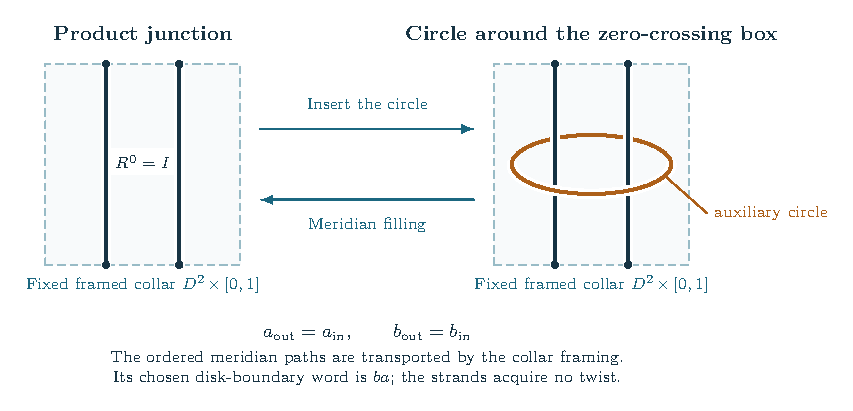
\includegraphics[width=.94\linewidth,keepaspectratio]{../book/figures/zero-circle-junction.pdf}
\caption{A crossing circle is added around two straight strands in a fixed framed collar. Meridian filling removes it. The transported based meridians satisfy \(a_{\mathrm{out}}=a_{\mathrm{in}}\) and \(b_{\mathrm{out}}=b_{\mathrm{in}}\); their chosen disk-boundary word is \(ba\).}
\label{fig:strict-zero-circle-junction}
\end{figure}

The fixed access paths make these ordered equalities precise. They
are constructed in Section~\ref{gj:what-the-edge-equations-see-at-the-complete-bare-representation}; the figure records the collar without
choosing additional paths.

For a holonomy representation, the added meridian must be projectively
identity: its matrix must be a scalar. An eigenvalue ratio of one would
also permit a nontrivial parabolic matrix. Section~\ref{gj:a-unique-regular-zero-power-angular-saddle} excludes this
ambiguity by exhibiting an auxiliary longitude with distinct eigenvalues.

The original crossing powers, writhe and integer

\begin{equation}\label{gj:2}
a(D)=-w(D)-\sum_v n_v.
\end{equation}

are unchanged. The added circles have filling parameter zero, so their preferred-longitude surgery correction \(p_v\ell_v^2\) also vanishes.

\begin{figure}
\centering
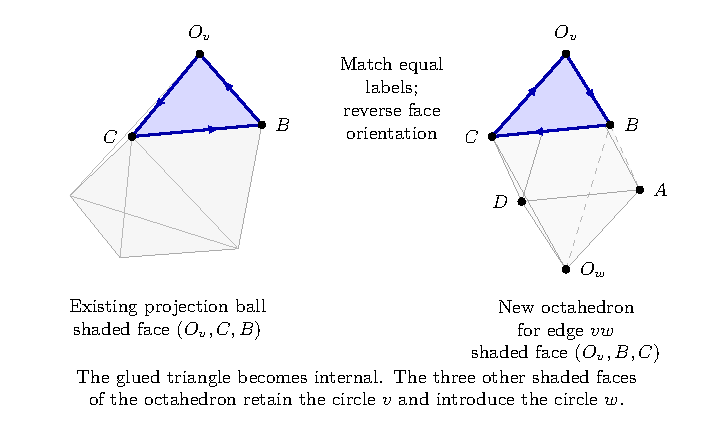
\includegraphics[width=.94\linewidth,keepaspectratio]{../book/figures/octahedral-page-attachment.pdf}
\caption{An ordered page attachment glues an edge block along a shaded triangle, retaining circle v and introducing circle w.}
\end{figure}

After the zero-power circles have been inserted, the
\href{https://sashakolpakov.github.io/murakamis_dream/notes/actual_all_circle_octahedral_decomposition.html}{ordered all-circle cut}
uses this attachment at every tree edge. The labels fix the page order.
The representation comparison below also permits a flat added
subdivision; it uses the original strict geometry to identify the knot
holonomy.

\section{A unique regular zero-power angular saddle}\label{gj:a-unique-regular-zero-power-angular-saddle}

Let a bare hub have \(m\ge3\) incident covariant labels \(x_1,\ldots,x_m\), with

\begin{equation}\label{gj:3}
0<x_j\le\tfrac12,\qquad
 \#\{j:x_j=\tfrac12\}\le1,\qquad
                         \sum_jx_j>1.
\end{equation}

The \href{https://sashakolpakov.github.io/murakamis_dream/notes/actual_main_meridian_component_pressure.html\#4-complete-physical-edge-labels-are-at-most-half}{complete physical-edge theorem}
and the \href{https://sashakolpakov.github.io/murakamis_dream/notes/actual_main_meridian_general_component_comparison.html\#8-the-original-complete-wire-window-and-complex-angular-parameters}{original wire-window argument}
give these conditions at the original complete strict optimizer. All physical labels are strictly below half except for the internal edge of the two-trivalent-hub component; that exception supplies at most one half label to either hub. Strict whole-hub support gives the final inequality. Hidden resolution labels are not included in \eqref{gj:3}.

The angular variable \(\tau\) describes the auxiliary disk longitude
by \(Q=e^{i\tau}\). The
\href{https://sashakolpakov.github.io/murakamis_dream/notes/actual_main_meridian_regular_circle_trace.html}{circle-incidence action}
is

\begin{equation}\label{gj:4}
b(x,\tau)=\int_0^x
       \log(2\cos(2\pi r)+2\cos\tau)\,dr-2J(x),
 \qquad J'(x)=\log(2\sin\pi x).
\end{equation}

Here \(J(0)=0\); its derivative specifies its continued branch. For \(\tau=-iy\), \(y>0\), every logarithm in the integral is real and finite. Put \(k=\tanh(y/2)\). Direct integration gives

\begin{equation}\label{gj:5}
b_\tau(x,-iy)=\frac{i}{\pi}
             \arctan\bigl(k\tan(\pi x)\bigr),
 \quad 0<x<\tfrac12,
\end{equation}

with value \(i/2\) at \(x=1/2\). Indeed
\[
 \int_0^x\frac{\sinh y}{\cosh y+\cos2\pi r}\,dr
   =\frac1\pi\arctan\bigl(k\tan\pi x\bigr).
\]
The zero-power first-charge equation is therefore

\begin{equation}\label{gj:6}
\sum_jb_\tau(x_j,\tau)-i=0
 \quad\Longleftrightarrow\quad
 \sum_j\arctan(k\tan\pi x_j)=\pi.
\end{equation}

A half label contributes \(\pi/2\). The left side is strictly increasing for \(0<k<1\), starts at zero or \(\pi/2\), and tends to \(\pi\sum_jx_j>\pi\). Thus \eqref{gj:6} has exactly one solution \(0<k<1\). Consequently

\begin{equation}\label{gj:7}
y=2\operatorname{arctanh}k>0,\qquad
 Q=e^{i\tau}=e^y=\frac{1+k}{1-k}>1.
\end{equation}

At least two labels are strictly below half. Differentiating \eqref{gj:6} shows that its derivative is strictly positive, so the angular Hessian is nonzero. The saddle and its selected logarithms extend holomorphically to a complex neighborhood of the fixed label tuple. The half-label case causes no singularity: the integrand of \eqref{gj:4} remains nonzero at \(y>0\), and \eqref{gj:6}'s derivative still has the contributions of the other labels.

In particular the new auxiliary longitude has distinct eigenvalues. If its meridian has similarity one and commutes with that longitude, it is projectively identity. The possible unipotent ambiguity at \(Q^2=1\) is absent.

\section{Exact elimination of the angular action}\label{gj:exact-elimination-of-the-angular-action}

Let \(V_m(\mathbf x)\) be the complete positive action of the whole hub.
It is defined by the \href{https://sashakolpakov.github.io/murakamis_dream/notes/actual_main_meridian_component_pressure.html\#1-complete-actions-boundary-variables-and-product-junctions}{ordered product kernel}: resolve the original ordered product by any fixed binary association, sum its cubic gate actions, and optimize the hidden complementary labels. The conditional optimizer is strict and has negative definite Hessian on the strict whole-hub support.

Then on \eqref{gj:3},

\begin{equation}\label{gj:8}
V_m(\mathbf x)=
 \underset{\tau}{\operatorname{stat}}
       \left\{\sum_jb(x_j,\tau)-i\tau\right\},
 \qquad \tau=-iy \text{ from (6)}.
\end{equation}

The equality includes its constant.

Here is one derivation retaining the exact complete normalization. The Newton factors are the finite polynomial basis used for the
tangle evaluation. For a factor with normalized index \(0<x<1/2\),
the logarithm of its Laurent coefficient at normalized exponent \(r\),
divided by the level, has rate

\begin{equation}\label{gj:9}
B_x(r)=J(2x)-2J(x)-J(x+r)-J(x-r),\qquad |r|\le x.
\end{equation}

The complete trace of a product has first Fourier charge one with coefficient exactly one. Its higher charges have strictly smaller rate; this follows from strict concavity of the positive coefficient convolution, or directly from the \href{https://sashakolpakov.github.io/murakamis_dream/notes/actual_main_meridian_regular_bare_trace.html}{regular bare-trace theorem}. The same exact complete trace is the positive binary-resolution sum. Therefore its rate is both \(V_m(\mathbf x)\) and

\begin{equation}\label{gj:10}
\max_{\substack{\sum_jr_j=1\\ |r_j|\le x_j}}
                               \sum_jB_{x_j}(r_j).
\end{equation}

The two expressions evaluate the same finite polynomial trace. Their
equality determines the local action with its constant and uses no
global quantum-volume asymptotic.

For \(0<x<1/2\),
\[
 B_x'(r)=\log\frac{\sin\pi(x-r)}{\sin\pi(x+r)}.
\]
The unique maximizer of \(B_x(r)+yr\) is

\begin{equation}\label{gj:11}
r=\frac1\pi\arctan\bigl(\tanh(y/2)\tan\pi x\bigr).
\end{equation}

Moreover

\begin{equation}\label{gj:12}
b(x,-iy)=\max_{|r|\le x}\{B_x(r)+yr\}.
\end{equation}

To verify the constant, at \(y=0\) both sides are
\(J(2x)-4J(x)\). Their \(y\)-derivatives are the same \(r\) by \eqref{gj:5} and \eqref{gj:11}. The constrained maximizer \eqref{gj:10} has common multiplier \(y>0\), determined by \(\sum r_j=1\). Equations \eqref{gj:10}--\eqref{gj:12} prove \eqref{gj:8}. A half label follows by continuity. Equivalently \(B_{1/2}(r)=0\), so its tilted maximum is \(y/2\), as also follows directly from \eqref{gj:4}.

For a cubic vertex one can avoid the finite trace altogether. The old action is

\begin{equation}\label{gj:13}
t(x_1,x_2,x_3)=
 \sum_{i<j}J(x_i+x_j)-\sum_iJ(x_i)-J(x_1+x_2+x_3-1).
\end{equation}

Writing \(a_j=\tan\pi x_j\), equation \eqref{gj:6} gives
\(k^2=(a_1+a_2+a_3)/(a_1a_2a_3)\).
The derivative of the right side of \eqref{gj:8} in \(x_j\) is

\begin{equation}\label{gj:14}
\log\frac{\cosh y+\cos2\pi x_j}{2\sin^2\pi x_j}
   =\log\frac{k^2+\cot^2\pi x_j}{1-k^2},
\end{equation}

which is exactly \(\partial_jt\). As \(\sum x_j\downarrow1\), \(y\to\infty\), and both actions tend to \(-2\sum_jJ(x_j)\). This proves the cubic identity with its absolute constant.

Both sides of \eqref{gj:8} are holomorphic near the fixed strict tuple. Their equality on an open real set proves equality of the continued germs. At the possible half label, use their holomorphic continuation from labels below half; both Hessians remain invertible there.

\section{The actual added longitude in the old prism geometry}\label{gj:the-actual-added-longitude-in-the-old-prism-geometry}

The previous section identifies actions. The following matrix calculation identifies the new circle inside the
original marked geometry. A white map is the full Möbius transition
between a white face in one projection copy and its partner in the
other copy. Its translation as well as its fixed points is retained.

In an ordinary output port of the bare product write
\[
 E=e^{2\pi ib},\qquad R=\frac1{1+\kappa},\qquad
 \kappa=e^{-f'(b)}.
\]
The \href{https://sashakolpakov.github.io/murakamis_dream/notes/actual_conway_general_mask_marked_filling.html\#4-actual-and-virtual-white-maps-for-every-mask}{marked product construction}
gives the universal white maps

\begin{equation}\label{gj:15}
W_1=\begin{pmatrix}1&E-1\\0&E\end{pmatrix},\qquad
 W_3=\begin{pmatrix}R&0\\1-E&ER\end{pmatrix}.
\end{equation}

They are the actual top and bottom white-face maps at an unmasked bare product. Through every original binary product, the full matrix identities give

\begin{equation}\label{gj:16}
W_{F,1}=W_{G,1}=W_{o,1},\qquad
 W_{F,3}=W_{G,3}=W_{o,3}
\end{equation}

in the original world frame. Consequently the same ordered side word is seen at every port of that hub.

Insert the zero-crossing box in the original disk frame. Its primitive disk-longitude path crosses these two white sides, giving \(W_1^{-1}W_3\), up to the inversion required when the circle's orientation is reversed. The determinant-one normalization is

\begin{equation}\label{gj:17}
P=\frac1R W_1^{-1}W_3,\qquad
 \operatorname{tr}P
   =2-\frac{4\sin^2\pi b}{R}.
\end{equation}

This is the same \(W_1^{-1}W_3\) disk word used at the corresponding end of an all-circle edge; it is not a trace chosen to fit \eqref{gj:6}.

The response metric records the ordered quadrilateral shape at a
product boundary. Its coordinate \(X_{\mathrm{met}}\) is distinct
from the exponential wire variable \(X_e=e^{2\pi ix_e}\). It is
\[
 X_{\mathrm{met}}^2=\frac{1+\cot^2\pi b}{1+\kappa}.
\]
Therefore

\begin{equation}\label{gj:18}
\operatorname{tr}P=2-\frac4{X_{\mathrm{met}}^2}.
\end{equation}

At a boundary incidence with covariant label \(x\), the ordinary output is \(b=1-x\), and the conditional action satisfies \(f'(b)=-\partial_xV_m\). Using \eqref{gj:14}, valid at any valence by the envelope identity \eqref{gj:8}, gives

\begin{equation}\label{gj:19}
X_{\mathrm{met}}^2
 =\frac1{\sin^2\pi x\,[1+\exp(\partial_xV_m)]}
 =\operatorname{sech}^2(y/2)=1-k^2.
\end{equation}

Thus

\begin{equation}\label{gj:20}
\operatorname{tr}P=-2\cosh y=-(Q+Q^{-1}).
\end{equation}

This proves that the actual added longitude has the regular eigenvalues required by the angular saddle. The proof retains the old group word, and shows why a bare hub has a common \(Q\) across all its pages.

When an incidence is viewed through its physical turn, the old identity
\(T W_{j+1}(E,R)=W_j(E^{-1},1-R)T\)
takes the \(W_1^{-1}W_3\) word to the appropriate inverse of the \(W_2^{-1}W_0\) word. Its trace is unchanged. The auxiliary flag may be selected on the eigenvalue \(-Q\), \(Q>1\); the main meridian flags are not changed by this auxiliary choice.

\section{What the edge equations see at the complete bare representation}\label{gj:what-the-edge-equations-see-at-the-complete-bare-representation}

Pull the original complete holonomy back along the exact filling quotient obtained in Section~\ref{gj:the-literal-insertion}. This gives a representation of the enlarged augmented link with every newly added meridian equal to identity. It is a representation-theoretic pullback; no assertion that the drilled link carries this metric is needed.

\subsection{The marked zero-crossing collar}\label{gj:the-marked-zero-crossing-collar}

Choose the box in a framed ball \(D^2\times[0,1]\), with its two strands
\(\{p_1,p_2\}\times[0,1]\). Choose a basepoint \(z_*\in\partial D^2\),
an ordered pair of disjoint access paths from it to small circles around
\(p_1,p_2\), and transport that entire system by the product framing.
Orient and name the resulting based puncture loops \(a,b\) so that
the oriented disk-boundary word is \(ba\). The boundary basepath is
\(\{z_*\}\times[0,1]\). Transport across this literal zero-crossing box gives

\begin{equation}\label{gj:22c}
a_{\mathrm{out}}=a_{\mathrm{in}},\qquad
                        b_{\mathrm{out}}=b_{\mathrm{in}}.
\end{equation}

These are equalities in the based fundamental group, before taking any
representation. No permutation of punctures, turn of an access path,
or power of the disk-boundary curve is included.

Place the new auxiliary circle at the disk boundary in the middle
of this collar, with the original disk framing. Its longitude is
the parallel copy of that boundary and retains the based word \(ba\).
The meridian filling deletes the auxiliary circle and returns exactly
the framed collar just described. Its quotient on fundamental groups
fixes \(a,b\), their access paths, and the boundary basepath. Thus it
also fixes the ordered maps by which this collar is joined to all
earlier and later product factors. This remains true when there are
several child factors: transport the same system through them in
their recorded order. It never requires the factors to commute.

For comparison with a pair of projection faces, transport the framed
loops to the face basepoints along the original specified paths.
If the old transport is \(C_0\), \eqref{gj:22c} becomes the simultaneous
conjugacy \(C_0aC_0^{-1}=a'\), \(C_0bC_0^{-1}=b'\).
Reading the other side of a puncture changes the corresponding
native generator to its inverse. Those inversions are recorded
explicitly in \eqref{gj:22b} below; they do not change \eqref{gj:22c} into a braid.
This is the marked van Kampen statement used at every added seam.
Only a retained nonzero half twist changes \eqref{gj:22c}, by the separately
calibrated Hurwitz action.

A port here is the ordered quadrilateral chart supplied by the
original cell construction. It is not assumed to be a new
four-punctured topological boundary. On a physical turn edge use its
original coordinate \((0,\infty,1,R)\) and its phase \(E=e^{2\pi ix}\).
This is the transported physical-edge frame from the last paragraph
of Section~\ref{gj:the-actual-added-longitude-in-the-old-prism-geometry}; its phase is the reciprocal of the ordinary-output
phase \(e^{2\pi ib}\), with the corresponding change \(R\mapsto1-R\).
At \(M=1\) the four \href{https://sashakolpakov.github.io/murakamis_dream/notes/actual_all_circle_geometric_characteristic.html\#2-the-local-face-maps}{native all-circle white matrices} are exactly the universal old \(W_j(E,R)\), projectively. This follows by putting \(m=1\) in the explicit native chart, without specializing the auxiliary eigenvalues to one.

The two disk words have normalized traces \(-\beta,-\gamma\), where

\begin{equation}\label{gj:21}
\beta=\frac{2R-(E+E^{-1})}{1-R},\qquad
 \gamma=\frac{2-(E+E^{-1})-2R}{R}.
\end{equation}

At an inserted hub these are supplied by \eqref{gj:20}; at an original circle they are its original marked longitude trace. Eliminating \(R\) yields

\begin{equation}\label{gj:22}
A=\frac{4-\beta\gamma}{\beta+\gamma+4},
 \qquad A=E+E^{-1},
\end{equation}

which is exactly the all-circle edge equation at \(M=1\). Thus the old phase is one of its two reciprocal roots. The native white maps retain \(E\) itself, not just \(E+E^{-1}\); the existing native/character comparison identifies the all-circle source variable with that \(E\).

All character-chart denominators are units at this point: \(\beta,\gamma\ge2\), \(E\ne1\), and the displayed original port vertices are distinct. The allowed value \(E=-1\) on the two-hub half edge does not cause a character-matrix singularity. In that case the edge quadratic may ramify over its endpoint parameters; one must use the full stationary branch or another local coordinate, not assert that \(E\) is a simple quadratic root.

Indeed \(E=-1\) gives

\begin{equation}\label{gj:22e}
(\beta-2)(\gamma-2)=16
 \quad\Longleftrightarrow\quad
 X_{\mathrm{met},v}^{\,2}+X_{\mathrm{met},w}^{\,2}=1,
\end{equation}

by \eqref{gj:18}. This is the possible half-edge fold of the old geometry.
The normalized matrices and the two irreducible puncture pairs
below remain regular there.

Here is the boundary-group comparison, including the tuple that has to be retained. First choose the normalized native matrix representatives for the four old projective white maps. In terms of the raw universal representatives used in \eqref{gj:15}, their scalar factors are respectively

\begin{equation}\label{gj:22d}
E^{-1},\quad E^{-1},\quad
                [E(1-R)]^{-1},\quad (ER)^{-1}.
\end{equation}

Each normalized matrix has determinant \(E^{-1}\) at \(M=1\).
The raw universal representatives do not all have that determinant:
in particular the factors involving \(R\) and \(1-R\) cannot be
discarded when taking an SL trace. With \(W_j\) now denoting these
normalized native representatives, put in each original edge frame

\begin{equation}\label{gj:22a}
N_j=W_{j-1}^{-1}W_j,\qquad
 (A,B,C,D)=(N_3,N_0,N_1,N_2)
\end{equation}

with the subsequent determinant-one puncture normalizations from the
all-circle chart. These subsequent powers of \(M\), not the scalar
factors in \eqref{gj:22d}, are one at \(M=1\). Thus every \(N_j\) has determinant
one and trace two. The actual page table is

\begin{equation}\label{gj:22b}
\begin{array}{c|c|c|c}
\text{end}&(a,b)&(a',b')&ba=b'a'\\ \hline
v&(B,A)&(C^{-1},D^{-1})&AB\\
w&(B^{-1},C^{-1})&(A,D)&(BC)^{-1}.
\end{array}
\end{equation}

The entries refer to paths, with the inverse on each puncture determined by its side of the disk. They are exactly the table of the literal all-circle cut, not a new identification of equal traces.

To apply that table to the old holonomy, first insert the zero-crossing box in the actual diagram, before assigning matrices. The main strands and their ordered endpoint paths are unchanged. Add the new circle and perform the literal projection/disk cut. The filling quotient takes every old main meridian and its old basepath to itself and kills the new circle meridian. In particular the four small corner paths reduce to the original consecutive-white words in \eqref{gj:22a}. A white face split by the added cut retains the same transport on both of its pieces: crossing the extra cut and returning differs by the new meridian, whose image is identity. This is also the full-map invariant \eqref{gj:16} through every prism of the original product. Thus the developed four white transitions of the pulled-back representation are exactly the four \(W_j\) already compared above.

The paths across the added disk pages are still the paths of this cut. By van Kampen they intertwine both generators in the appropriate row of \eqref{gj:22b}, with precisely the displayed inversions; the product column is their original primitive disk boundary. The inserted box has no crossing, so no Hurwitz exchange is made at its distinguished seam. The old retained half twists keep their original exchanges.

At \(M=1\), either input pair in \eqref{gj:22b} is irreducible. Both punctures have trace two, and the products in the two rows have traces \(-\beta\) and \(-\gamma\), respectively, with \(\beta,\gamma\ge2\). Their irreducibility obstructions are \((\beta+2)^2\ne0\) and \((\gamma+2)^2\ne0\). Two intertwiners of either full ordered pair differ by its scalar centralizer. Therefore the pulled-back page transport equals the native pure transport in PGL. At an original odd seam the same argument is applied after the already calibrated full Hurwitz action. The corner flags on the main cusp are the old parabolic flags, and the extra auxiliary flags are chosen from \eqref{gj:20}; these choices do not alter a group generator.

All white and shaded generators of the cut now agree, in their original tree frames. This proves equality of the complete representations, not only of the local character triples or the main-cusp translation. It identifies the selected all-circle algebraic point with the pullback of the original bare-tree holonomy. The newly introduced ideal vertices need not form positive tetrahedra in this pulled-back representation. In particular an edge with \(E=-1\) can make that added subdivision flat. No metric on the enlarged unfilled exterior is asserted or required.

\section{Stationary elimination at a nonparabolic main meridian}\label{gj:stationary-elimination-at-a-nonparabolic-main-meridian}

Let \(t\) be the actual main deformation parameter, \(M=e^{\pi it}\).
In the existing strict-tree filtered action it enters only through

\begin{equation}\label{gj:23}
\sum_{e\in\mathcal E_T}
       \{2J(x_e)-J(x_e+t)-J(x_e-t)\}
       +\frac{\pi i a(D)}2t^2.
\end{equation}

It does not enter the old bare tensor action or its hidden resolution wires.

The enlarged all-circle action replaces a bare hub by
\(\sum_jb(x_j,\tau_v)-i\tau_v\), with \(n_v=0\).
Eliminating \(\tau_v\) by \eqref{gj:8} returns exactly the old whole-hub action, including its constant, for complex physical wires in the regular neighborhood. The edge set and \eqref{gj:23} do not change, and neither does \(a(D)\). Hence the two full critical-value germs are equal after stationary elimination.

The new angular Hessian at each bare hub is nonzero. To state the
comparison precisely, first eliminate the old hidden binary-resolution
variables. Their conditional Hessian is invertible by strictness.
Let \(z\) collect the remaining original variables and let
\(\tau_{\mathrm{new}}\) collect only the added angular variables.
The enlarged Hessian has blocks

\begin{equation}\label{gj:23a}
H_{\mathrm{new}}=
 \begin{pmatrix}
 H_{zz}&H_{z\tau}\\ H_{\tau z}&H_{\tau\tau}
 \end{pmatrix},\qquad
 H_{\mathrm{old,red}}
   =H_{zz}-H_{z\tau}H_{\tau\tau}^{-1}H_{\tau z}.
\end{equation}

The block \(H_{\tau\tau}\) is diagonal over the added hubs, with
nonzero entries from \eqref{gj:6}. Equality \eqref{gj:8} identifies its Schur
complement with the old reduced Hessian. The original full Hessian
and its eliminated hidden block are invertible, so
\(\det H_{\mathrm{new}}
 =\det H_{\tau\tau}\det H_{\mathrm{old,red}}\ne0\).
No individual edge Hessian is inverted, including at \eqref{gj:22e}.

The enlarged analytic branch therefore exists with all the original
logarithms retained. Original sufficiently long fillings keep their
auxiliary \(Q_v^2\ne1\); every added zero-power circle has
\(Q_v^2\ne1\) by \eqref{gj:7}, and this persists near the complete branch.

By Section~\ref{gj:what-the-edge-equations-see-at-the-complete-bare-representation} this branch reconstructs the original filled knot representation, rather than only an algebraic solution of the slope eigenvalue equations. Near the old augmented complete point the original auxiliary deformation is fixed by its primitive peripheral rows. Equality at completeness and the marked gluing/representation local inverse identify the two nearby deformations. The original sufficiently long filling point lies on that same small branch. There every original filled circle, as well as every added zero circle, has \(Q_v^2\ne1\); the filling words are projectively identity by Section~\ref{gj:a-unique-regular-zero-power-angular-saddle}. The nondegenerate main-meridian branch is then the geometric germ of the original filled knot.

The all-circle squared longitude identity is a rational identity on its integral source variety. It extends to this regular representation, including the half-edge fold, without solving for an individual edge root. The added zero fillings contribute no surgery exponent, the Seifert sign is that of the same original complete knot, and stationary elimination leaves the effective longitude unchanged. Consequently

\begin{equation}\label{gj:24}
L_{\mathrm{geom}}(M)
   =-M^{a(D)}
      \prod_{e\in\mathcal E_T}
                \frac{M^2-X_e(M)}{1-M^2X_e(M)}
\end{equation}

on the original strict-tree filled branch, with \(X_e=e^{2\pi ix_e}\).

This proves the theorem on the geometric germ of the original
filled knot. The same physical edges occur before and after the
zero-circle elimination, and the added circles contribute neither
a crossing power nor a preferred-longitude shear.

The geometric identification uses the full ordered boundary-group
comparison in Section~\ref{gj:what-the-edge-equations-see-at-the-complete-bare-representation}. The equality of actions in Section~\ref{gj:exact-elimination-of-the-angular-action} supplies
the stationary branch, while the marked face maps identify its
representation. These are distinct parts of the proof. The established
strict-tree quantum estimates retain their existing long-filling
hypotheses; this argument adds no estimate for short fillings.

\section{The geometric factor selected by the actual recurrence}\label{gj:the-geometric-factor-selected-by-the-actual-recurrence}

The geometric theorem identifies the curve already selected by the
full asymptotic expansion of the original strict-tree invariant.
This extends the operator consequence beyond trees whose junctions
all carry crossing circles. It requires no quantum estimate for the
newly drilled diagram: the quantum source remains the original
strict presentation.

Fix an oriented strict ordered Conway knot presentation \(D\), with
its original cut, endpoint orders, framing and signed integral
crossing powers. Assume the powers are independently sufficiently
long for the \href{https://sashakolpakov.github.io/murakamis_dream/notes/actual_main_meridian_filled_volume.html}{filled-meridian theorem}
and the geometric theorem above. The entire diagram and every power
are fixed before \(N\) tends to infinity. All original knot-pattern
and absence-of-internal-component qualifications remain in force.
Both level parities and all sufficiently large composite levels are
included.

Write \(F_N(M)\) for the actual zero-framed reduced ADO invariant,
with

\begin{equation}\label{gj:O1}
q_N=e^{\pi i/N},\qquad M=-q_Nx,\qquad F_N(1)=K_N(K).
\end{equation}

Here \(x\) is the raw highest-weight parameter, distinct from an
internal normalized index \(x_e\). The marked complete meridian is
\(M=1\), and \(X_e=e^{2\pi ix_e}\) denotes the original physical-edge
variable.

Let

\begin{equation}\label{gj:O2}
P(q,M,T)=\sum_{j=0}^{d}a_j(q,M)T^j,\qquad
 a_j\in\mathbb C(q,M),\qquad TM=qMT,
\end{equation}

be any specified nonzero fixed operator that annihilates the whole
function \(F_N(M)\) at every sufficiently large level. The shift \(T\)
replaces \(M\) by \(qM\). Such an actual all-level annihilator exists
by the \href{https://sashakolpakov.github.io/murakamis_dream/notes/finite_sum_annihilator.html}{finite-sum construction}; it is not
defined by fitting the complete values or adjoining a desired factor.
An operator with negative shift powers can first be multiplied by
a power of \(T\).

Clear fixed rational denominators, remove the common \(q-1\)
valuation of the coefficients, and denote the resulting first nonzero
classical symbol by \(P_0(M,L)\). Let
\(A_{\mathrm{geom},\mathbb C}(M,L)\) generate the Laurent prime of the
actual geometric eigenvalue germ through \((1,-1)\), in the preferred
meridian and longitude of the original knot. The longitude coordinate
is its eigenvalue on the \(M\) line, equivalently the inverse
eigenvalue on the source \(M^{-1}\) line.

Then

\begin{equation}\label{gj:O3}
\boxed{\displaystyle
 A_{\mathrm{geom},\mathbb C}(M,L)\mid P_0(M,L)
 \quad\text{in }\mathbb C[M^{\pm1},L^{\pm1}].}
\end{equation}

Thus every genuine all-level annihilator has the same selected
irreducible geometric factor in its first classical symbol.

\subsection{Proof and normalization}\label{gj:proof-and-normalization}

The \href{https://sashakolpakov.github.io/murakamis_dream/notes/actual_main_meridian_filtered_characteristic.html}{filtered characteristic theorem},
Sections 2--6, already applies to the full strict long-filling class,
including arbitrary bare components. It proves the complete
microscopic expansion with its degree filtration on all the finitely
many translated parameter charts needed by \eqref{gj:O2}. This shifted-chart
statement follows from the exact source and its endpoint estimates,
not from continuation of an asymptotic formula on a single disk.

The normalized full state is

\begin{equation}\label{gj:O4}
\mathcal Z_N(s)=\frac{F_N(q_N^s)}{F_N(1)H_N(s)},\qquad
 H_N(s)=\frac{\sin\pi s}{N\sin(\pi s/N)}.
\end{equation}

It retains the exact modified-dimension gauge

\begin{equation}\label{gj:O5}
d_N(M)=\eta_N\frac{M-M^{-1}}{M^N-M^{-N}},\qquad
 d_N(1)=\eta_N/N,\qquad
 \frac{d_N(q_N^s)}{d_N(1)}=H_N(s)^{-1}.
\end{equation}

Here \(\eta_N=i^{N+3}\). Put \(f(M)=M-M^{-1}\). The operator on the
full state has shift coefficients

\begin{equation}\label{gj:O6}
\widetilde a_j(q,M)
 =a_j(q,M)(-1)^j\frac{f(M)}{f(q^jM)}.
\end{equation}

Multiplication on the left by \(\prod_{j=1}^{d}f(q^jM)\)
gives the first classical symbol \(f(M)^dP_0(M,-L)\). The meridian
divisor and shift sign are therefore retained before the formal cancellation.

The filtered theorem defines the selected critical value \(S(t)\)
using the original phase and the insertion

\begin{equation}\label{gj:O7}
\sum_{e\in\mathcal E_T}
 [2J(x_e)-J(x_e+t)-J(x_e-t)]
 +\frac{\pi i a(D)}2t^2.
\end{equation}

Its expansion has coefficient of order \(N^{-r}\) of degree at
most \(r+1\) in \(s\). The top-degree coefficients come from \(S\);
lower Gaussian amplitudes cannot change them. With
\(\mathcal S(u)=\pi i[S(u/(\pi i))-S(0)]\), the exact operator
equation and this filtration give the formal domain identity

\begin{equation}\label{gj:O8}
f(e^u)^dP_0(e^u,-e^{\mathcal S'(u)})=0.
\end{equation}

The full argument, including injectivity of the substitution
\(u=hs\), is in
\href{https://sashakolpakov.github.io/murakamis_dream/notes/actual_all_circle_geometric_characteristic.html\#11-the-geometric-factor-of-an-actual-quantum-recurrence}{the all-circle operator proof},
Section~\ref{gi:all-orders-shifted-charts-and-the-geometric-branch}. That argument depends on the filtered source expansion
and the exact gauge, not on the absence of bare vertices. The
nonzero series \(f(e^u)^d\) can be cancelled in this proved integral
domain identity.

The new geometric input identifies its entire selected germ:

\begin{equation}\label{gj:O9}
-e^{\mathcal S'(\log M)}
 =-M^{a(D)}\prod_{e\in\mathcal E_T}
              \frac{M^2-X_e(M)}{1-M^2X_e(M)}
 =L_{\mathrm{geom}}(M).
\end{equation}

The zero-circle elimination above preserves the whole critical-value
germ and the original physical-edge set. Its ordered boundary-group
anchor identifies the original filled geometric representation.
The preferred-longitude sign is fixed at that filled knot point.
Thus \eqref{gj:O9} is not inferred from the cusp tangent or from a choice among
unmarked exponentiated solutions.

It follows that \(P_0\) vanishes on the geometric eigenvalue germ.
Its Laurent evaluation kernel is a nonzero prime and contains no
nonzero polynomial in \(M\) alone, because \(M\) varies. It is
therefore a height-one prime in a Laurent polynomial unique
factorization domain, proving \eqref{gj:O3}.

If the operator coefficients lie in \(\mathbb Q(q,M)\), contract
that same germ prime to \(\mathbb Q[M^{\pm1},L^{\pm1}]\). Its
irreducible generator divides the rational symbol. Its complex
factorization contains the selected geometric factor and any
conjugate factors required over \(\mathbb Q\); an individual complex
component need not itself be defined over \(\mathbb Q\).

\section{Transfer to presentations with net twists and arbitrary closures}\label{gj:transfer-to-presentations-with-net-twists-and-arbitrary-closures}

The conclusion is intrinsic to the zero-framed knot with its marked
peripheral curves. Suppose the
\href{https://sashakolpakov.github.io/murakamis_dream/notes/actual_conway_net_twist_volume.html}{ordered net-twist reduction} gives
an actual ambient isotopy from the input knot to a strict knot
presentation covered by Section~\ref{gj:the-geometric-factor-selected-by-the-actual-recurrence}. The isotopy carries the knot
orientation, meridian, preferred zero-linking longitude and cut mark.
Correcting any transported ribbon framing to zero gives exactly the
same reduced ADO function \(F_N(M)\) at every level and every
meridian value where it is defined. Its rational continuation is
therefore the same function as well.

The geometric eigenvalue germ is also the same under this marked
isotopy. An actual all-level operator for the input family thus
satisfies the hypotheses of Section~\ref{gj:the-geometric-factor-selected-by-the-actual-recurrence} for that same intrinsic
family. Its first classical symbol contains the selected geometric
factor. This transfers the factor statement without identifying
presentation-specific recurrence formulas or their unreduced
polynomial representatives.

The same argument applies to the
\href{https://sashakolpakov.github.io/murakamis_dream/notes/actual_conway_arbitrary_closure_volume.html}{arbitrary-closure reduction}
when its hypotheses yield one covered strict knot factor and only
unknot factors. In particular, under its long surviving-factor
hypotheses, a hyperbolic knot input has exactly that form. Removing
the exhibited unknot summands is an actual orientation-preserving
ambient isotopy. The preferred peripheral pair is carried by the
induced map of exteriors. No multiplicativity assertion for quantum
growth over connected sums is required.

For a fixed original expression there are finitely many recorded
reduction and parity branches. If a uniform net-weight statement is
desired, take the maximum of the strict source and geometric
thresholds over those finitely many possible strict outputs. The
threshold concerns their surviving signed net powers. Large
individual powers that cancel to a short surviving power do not
satisfy it. This does not assert that an earlier, smaller
complete-value threshold automatically supplies the stronger
moving-meridian hypotheses.

The integer \(a(D)\) and the individual edge factors in \eqref{gj:O9} are
computed on the covered strict diagram. They are not claimed to
equal those read from an unreduced input presentation term by term.
The preferred geometric longitude and its selected irreducible
factor are the intrinsic objects that transfer.

The conclusions concern one irreducible geometric factor, not the
full A-polynomial, its multiplicity, or an equality of quantum
operator ideals. They do not provide a fixed-\(M\) large-level WKB
theorem, nonvanishing through ordinary-color resonances, or a
general short-twist theorem. The wider quantitative all-circle
alternatives remain available under their own source and geometric
hypotheses; this section neither narrows those results nor extends
them to arbitrary short bare-junction fillings.

\chapter{Volume limits from the degree and twist at each circle}
\label{app:directed-circle-messages}\label{dk:volume-limits-from-the-degree-and-twist-at-each-circle}

Start with a fixed finite ordered tree of two-strand integer braids, with
at least one edge and one crossing circle at every vertex. Turn each child tangle through its
specified quarter-turn before stacking it at the parent, and use the
original cylindrical closure. The
\href{https://sashakolpakov.github.io/murakamis_dream/notes/actual_all_circle_quantitative_volume.html\#the-knot-construction}{literal construction and strand test}
retain the endpoint frames and require one closed main knot, with no
component closed inside an intermediate tangle.

Write \(d_v\) for the degree of vertex \(v\), and \(n_v\) for its signed
number of half-twists. A sufficient condition for the volume limit is
\[
 \boxed{\qquad d_v\ge2^{28}\quad\text{or}\quad |n_v|\ge2^{27}
                       \qquad\text{at every vertex}.\qquad}
\]
The alternative can be chosen separately at each vertex. High-degree
vertices may retain any fixed signed powers, including zero and small
nonzero powers. If the strand test gives a knot \(K\), its original
complement is hyperbolic and
\[
 \lim_{N\to\infty}\frac{2\pi}{N}\log|K_N(K)|
                       =\operatorname{Vol}(S^3\setminus K).
\]
Both level parities are included. The tree, powers and degrees are fixed
before \(N\) tends to infinity. The constants are coarse sufficient
bounds; they make no claim about the shortest possible twists.

The more general criterion below assigns a real-decay bound to each
subtree polynomial. Dividing by that polynomial's exact value at zero
retains its complex scalar and isolates the contribution of the next
trace. Different edges may use different bounds. The final vertex has
no outgoing polynomial, so it need not pay the extra loss needed to
send one to a parent. This distinction also gives a short-power star
outside both the earlier summed and uniform local tests.

Section~\ref{dk:sec-8} explains how to retain arbitrarily many prescribed short
powers: add an even stack of sufficiently long terminal tangles at every
vertex of a fixed ordered knot core. Their endpoint pairing preserves
the knot condition, although the resulting knot type can change. The
proof estimates the actual finite invariant throughout; it does not
assume that a proposed global critical point dominates.

\section{The directed criterion}\label{dk:sec-1}

Put

\begin{equation}\label{dk:eq-1}
\begin{gathered}
a_0=\frac1{2\pi},\qquad k_0=2^{-16},\qquad
 R_0=\frac18,\qquad b_0=2^{-11},\qquad\\
 r_0=\frac1{16},\qquad t_0=2^{-14},\qquad
 \chi=1-\cos r_0.
\end{gathered}
\end{equation}

The parent-variable rectangle is

\begin{equation}\label{dk:eq-2}
\mathcal R=\{u:|\Re u|\le R_0,\ |\Im u|\le b_0\}.
\end{equation}

Choose any vertex as root and direct all edges toward it. For every
nonroot vertex choose a number

\begin{equation}\label{dk:eq-3}
0<c_v<k_0,
 \qquad
 \delta_v=\min\left\{\frac{b_0}2,
               \frac{c_v\chi}{4(1+c_v)}\right\}.
\end{equation}

These are parameters of the criterion. They can differ at every edge.
They are not asymptotic quantities to be inferred from the invariant.

Write \(q_v=1\) at a nonroot vertex and \(q_v=0\) at the root. If \(\mathrm{Ch}(v)\) is the
set of children, define

\begin{equation}\label{dk:eq-4}
\begin{aligned}
 a_v&=\frac{d_v}{2\pi},& b_v&=\frac{n_v}{2\pi},&
 D_v&=a_v-i b_v,\\
 A_v&=\frac2{\pi^2}
       \left(q_vk_0+\frac12\sum_{w\in\mathrm{Ch}(v)}c_w\right),&
 B_v&=16q_v+|\mathrm{Ch}(v)|,&
 C_v&=B_v+\frac{b_v^2}{4A_v}.
\end{aligned}
\end{equation}

There is at least one incidence at every vertex, so \(A_v,B_v\) are positive.
Let

\begin{equation}\label{dk:eq-5}
\delta_v^{\mathrm{in}}
      =\min\bigl(\{b_0\}\cup
                     \{\delta_w:w\in\mathrm{Ch}(v)\}\bigr)
\end{equation}

and set

\begin{equation}\label{dk:eq-6}
y_v=\min\left\{
 \frac{\delta_v^{\mathrm{in}}}2,
 \frac{t_0|D_v|}{4C_v},
 \frac{A_v\pi^2}{8(\pi|b_v|+t_0|D_v|)},
 \sqrt{\frac{A_v\pi^2}{8B_v}}
 \right\}.
\end{equation}

Finally define two action quantities

\begin{equation}\label{dk:eq-7}
\beta_v=\frac{210}{361}\frac{a_v}{|D_v|^2},
 \qquad
 \eta_v=\min\left\{
 \frac12t_0|D_v|y_v,
 \frac12A_v\pi^2,
 A_vr_0^2,
 \frac18a_vr_0^2
 \right\}.
\end{equation}

The criterion consists of the strict inequalities

\begin{equation}\label{dk:eq-8}
\boxed{\quad t_0|D_v|\ge2,\qquad
                 \beta_v<\frac{\eta_v}{2}\quad
                      \text{at every vertex},\quad}
\end{equation}

and, only at nonroot vertices,

\begin{equation}\label{dk:eq-9}
\boxed{\qquad
       \beta_v<(k_0-c_v)\chi.\qquad}
\end{equation}

It is a finite elementary test in the degrees, signed powers, root and
positive numbers \(c_v\). It uses no value of an unknown quantum invariant
and no assumed dominance of a global saddle. Its quantities are local:
\(A_v\) and the available strip depend on the child budgets, while the exact
child scalar will be divided out rather than estimated.

Use the original reduced-state normalization
\(q_N=e^{\pi i/N}\), \(M=-q_Nx=q_N^s\), and \(F_N(1)=K_N\).
The raw highest-weight parameter \(x\) here is distinct from a normalized
wire coordinate. The \href{https://sashakolpakov.github.io/murakamis_dream/notes/kashaev_ado_pointing.html}{pointing theorem} fixes this
ADO invariant and its zero framing.

\textbf{Theorem.} If \eqref{dk:eq-3}, \eqref{dk:eq-8}, and \eqref{dk:eq-9} hold, the actual reduced state has

\begin{equation}\label{dk:eq-10}
\frac{F_N(q_N^s)}{F_N(1)A_N(s)H_N(s)}
                  =1+O_{\mathcal T,\mathbf n,R}(N^{-1}),
             \qquad |s|\le R<1,
\end{equation}

where

\begin{equation}\label{dk:eq-11}
H_N(s)=\frac{\sin\pi s}{N\sin(\pi s/N)},\qquad
 A_N(s)=q_N^{a(D)s^2/2},\qquad a(D)=-w(D)-\sum_vn_v.
\end{equation}

Its complete values are nonzero for all sufficiently large levels and

\begin{equation}\label{dk:eq-12}
\lim_{N\to\infty}\frac{2\pi}{N}\log|K_N(K)|
                      =\operatorname{Vol}(S^3\setminus K).
\end{equation}

Both level parities and the original normal channels are retained.
The proof identifies the same original filled critical value as the
marked geometric completion. It does not use a sum of independent
subtree volumes.

\section{An actual conditional kernel on a rectangle}\label{dk:sec-2}

The fixed Newton polynomials are

\begin{equation}\label{dk:eq-N1}
\begin{gathered}
 d=N-1,\qquad c_j=2\cos((2j+1)\pi/N),\qquad
 S_k=\prod_{r=1}^k2\sin(\pi r/N),\\
 e_k(z)=S_k^{-2}\prod_{j<k}(c_j-z),\qquad 0\le k<N.
 \end{gathered}
\end{equation}

Let \(\mathcal T_N(2\cos\theta)=2\cos(N\theta)\), and put
\(P_\sigma(z)=\mathcal T_N(z)+2\cos(2\pi\sigma)\). The normalized
polynomial trace is

\begin{equation}\label{dk:eq-N2}
\phi_\sigma(F)=(-1)^dN^2[z^d]\operatorname{rem}_{P_\sigma}F,
 \qquad \phi_\sigma(e_i e_j)=\mathbf1_{i+j=d}.
\end{equation}

The remainder has degree less than \(N\). This is the full polynomial
functional, including its derivative values when roots coalesce.
The \href{https://sashakolpakov.github.io/murakamis_dream/notes/actual_main_meridian_turn_comparison.html}{typed turn theorem}
retains the paired factors

\begin{equation}\label{dk:eq-N3}
W_k(s)=\prod_{r=1}^k
     \left(1-\frac{\sin^2(\pi s/N)}{\sin^2(\pi r/N)}\right).
\end{equation}

After lowering the pairing \eqref{dk:eq-N2}, a physical turn gives the equal-index
weight \(\gamma_e(s)H_N(s)/W_k(s)\). The factor \(\gamma_e\) is the
original scalar prescribed by that edge's orientation type. It stays in
the exact scalar ledger.

For the edge action write

\begin{equation}\label{dk:eq-N4}
\begin{gathered}
 J(x)=\int_0^x\log(2\sin\pi v)\,dv,\qquad
 g(x)=J(2x)-4J(x),\qquad G_0=g(1/4),\\
 b(x,t)=\int_0^x\log(2\cos(2\pi v)+2\cos t)\,dv-2J(x),\\
 \psi(t,u)=\operatorname{stat}_x[b(x,t)+b(x,u)],
                       \qquad\psi(0,0)=2G_0.
 \end{gathered}
\end{equation}

The logarithms and stationary branch are continued from
\(x=1/4,t=u=0\). The finite factorial interpolation, the actual edge
contour and this phase are proved in
\href{https://sashakolpakov.github.io/murakamis_dream/notes/actual_all_circle_curvature_filling_limit.html}{the all-circle finite-sum theorem}.
Its polynomial estimates use
\href{https://sashakolpakov.github.io/murakamis_dream/notes/all_circle_uniform_newton_bounds.html}{the full Newton bounds}.
Use the exact full kernel

\begin{equation}\label{dk:eq-13}
K_N(t,u;s)=\sum_{k=0}^{N-1}
       e_k(-2\cos t)e_k(-2\cos u)\frac{H_N(s)}{W_k(s)}.
\end{equation}

The definitions of \(e_k,W_k\) and the fixed anti-diagonal trace metric are
unchanged. It is a polynomial of degree at most \(N-1\) in each of
\(-2\cos t\) and \(-2\cos u\), hence has trigonometric degree at most
\(N-1\) in either angle.
The paired factors and their inverses are bounded for fixed \(|s|\le R<1\).
Every inequality below permits a polynomial factor in N.

The \href{https://sashakolpakov.github.io/murakamis_dream/notes/actual_all_circle_local_message_volume.html\#two-full-kernel-bounds}{full-kernel real estimate} is

\begin{equation}\label{dk:eq-14}
|K_N(t,u;s)|\le C_RN^{A_R}
   e^{N\{2G_0-k_0[(1-\cos t)+(1-\cos u)]\}},
                 \qquad t,u\in[-\pi,\pi].
\end{equation}

The new estimate needed here is

\begin{equation}\label{dk:eq-15}
|K_N(t+iy,u;s)|\le C_RN^{A_R}
 e^{N\{\Re\psi(0,u)-k_0(1-\cos t)+16y^2\}},
 \quad u\in\mathcal R,\quad t\in[-\pi,\pi],\quad |y|\le b_0.
\end{equation}

Thus the parent compact is a long, thin rectangle, rather than the old
disk of radius \(2^{-12}\). The constant term is the actual conditional phase
\(\psi(0,u)\), not its upper bound \(2G_0+O(|u|^2)\).

Here is a proof from the original finite kernel. Split the indices into
\(I=[1/5,3/10]\) and its complement. The complementary full polynomial
has the established single-edge loss \(\eta_K=\pi/200\), including high
indices and their complete derivatives. Its ellipse bound is

\begin{equation}\label{dk:eq-16}
C_RN^{A_R}
       e^{N\{2G_0-\eta_K+|y|+|\Im u|\}}.
\end{equation}

The exact edge phase has, on the radius 1/4 bidisk,

\begin{equation}\label{dk:eq-17}
|\psi_{tt}+a_0|\le a_0/50,
 \quad |\psi_{uu}+a_0|\le a_0/50,
 \quad |\psi_{tu}|\le a_0/50,
 \quad \psi_t(0,u)=\psi_u(t,0)=0.
\end{equation}

In particular \(|\psi(0,u)-2G_0|\le |u|^2/10\). Hence \eqref{dk:eq-16} is smaller
than \eqref{dk:eq-15}: the sum \(b_0+b_0+(R_0^2+b_0^2)/10+2k_0\) is less
than \(\eta_K/2\). All these constants are independent of the tree.

For the retained indices write \(u=a+ib\). Their factors at \(a\) are positive.
If \(r_j=\cos(2\pi(j+1/2)/N)\), then \(r_j>-1/3\) and
\(r_j+\cos a>253/384\). Along \(|a|\le1/8,\ |b|\le2^{-11}\), the denominator
\(r_j+\cos(a+ib)\) has modulus greater than \(3/5\), and

\begin{equation}\label{dk:eq-18}
\left|\frac{d^2}{du^2}\log(r_j+\cos u)\right|
 =\left|\frac{-r_j\cos u-1}{(r_j+\cos u)^2}\right|<9.
\end{equation}

The first derivative at real a is real. Integrating vertically therefore
gives the actual finite-product estimate

\begin{equation}\label{dk:eq-19}
|e_k(-2\cos(a+ib))|
       \le e_k(-2\cos a)e^{5Nb^2},\qquad k/N\in I.
\end{equation}

At the other end retain the original product bound

\begin{equation}\label{dk:eq-20}
|e_k(-2\cos(t+iy))|
   \le e^2e_k(-2)e^{N[-\alpha\sin^2(t/2)+11y^2]},
                       \qquad \alpha>1/250.
\end{equation}

The positive retained sum at \((0,a)\) is bounded by a polynomial times
\(\exp(N\psi(0,a))\), uniformly for real \(|a|\le1/8\). This is the original
one-edge positive Laplace estimate: its unique critical wire is

\begin{equation}\label{dk:eq-21}
\tan^2(\pi x)=\frac1{1+\tan^2(a/2)},
\end{equation}

which stays in the interior of \(I\). Its second derivative stays negative
on this fixed real compact. Equations \eqref{dk:eq-19}--\eqref{dk:eq-20}, and the second bound
in \eqref{dk:eq-17}, consequently give

\begin{equation}\label{dk:eq-22}
|K_{N,I}(t+iy,u;s)|\le C_RN^{A_R}
 e^{N\{\Re\psi(0,u)-\alpha\sin^2(t/2)+11y^2+6b^2\}}.
\end{equation}

For \(|t|\ge1/8\),

\begin{equation}\label{dk:eq-23}
6b_0^2<\frac{\alpha}{2}\sin^2(1/16),\qquad
                         2k_0<\alpha/2.
\end{equation}

For example \(\sin(1/16)>1/(8\pi)\), \(\pi^2<10\) and \(\alpha>1/250\) already
prove the first inequality. This proves \eqref{dk:eq-15} in this range.

For \(|t|\le1/8\), the \href{https://sashakolpakov.github.io/murakamis_dream/notes/actual_all_circle_curvature_filling_limit.html}{canonical wire contour} gives the exact
nonzero edge asymptotic on the 1/4 bidisk. Both \(u\) and \(t+iy\) lie strictly
inside that disk. Integrating the first bound of \eqref{dk:eq-17} gives \eqref{dk:eq-15} there.
The original lattice currents and \eqref{dk:eq-16} are exponentially smaller.
In particular the full kernel, uniformly on this smaller rectangle
product, retains

\begin{equation}\label{dk:eq-24}
K_N(t,u;s)=N^{-3/2}a_e(t,u)e^{N\psi(t,u)}
                         (1+O_R(N^{-1})),
\end{equation}

with the original nonzero holomorphic leading amplitude and midpoint
normalization. The outside physical edge gamma is not included in \(a_e\).

\section{The exact recursion may be rooted anywhere}\label{dk:sec-3}

Lower the fixed Frobenius pairing at every vertex of the original closed
source. Every physical turn then identifies equal Newton indices and
retains its factor \(\gamma_e H_N/W_k\). The resulting finite scalar is a
sum over the original edge indices of a product of the original vertex
trace tensors. Choosing a root merely specifies the order of these
finite contractions. It does not move a cut through a tangle, commute
open operators or change a framing.

Consequently the \href{https://sashakolpakov.github.io/murakamis_dream/notes/actual_all_circle_local_message_volume.html\#the-full-finite-kernel-and-exact-recursion}{exact recursions}
hold for any chosen root:

\begin{equation}\label{dk:eq-25}
M_{v,N}(u)=\gamma_{e_v}(s)\,
 \mathcal D_{n_v,\sigma_v,N}^{(t)}
 \left[K_N(t,u;s)\prod_{w\in\mathrm{Ch}(v)}M_{w,N}(t)\right]
\end{equation}

at a nonroot vertex, and

\begin{equation}\label{dk:eq-26}
Z_N=\mathcal D_{n_o,\sigma_o,N}^{(t)}
                  \left[\prod_{w\in\mathrm{Ch}(o)}M_{w,N}(t)\right]
\end{equation}

at the root. The \href{https://sashakolpakov.github.io/murakamis_dream/notes/actual_main_meridian_exact_scalar.html}{original global closing, framing and reference factors},
and the original single reduced cut \(H_N\), remain outside \eqref{dk:eq-26}. Edge
gammas are counted once. The exact normal value \(\sigma_v=0\) and the moving
values \(\pm s\) retain their actual orientation types.

Each message is an even trigonometric polynomial of degree at most \(N-1\)
in \(u\), regardless of the subtree. There is no discarded-source error in
\eqref{dk:eq-25}--\eqref{dk:eq-26}.

\section{The phase class and the variable envelopes}\label{dk:sec-4}

The inductive analytic class is

\begin{equation}\label{dk:eq-27}
h_v(0)=h'_v(0)=0,\qquad h_v(-u)=h_v(u),\qquad
 |h_v''(u)+a_0|\le a_0/20,\quad u\in\mathcal R.
\end{equation}

The leading normalized amplitude \(\alpha_v(u)/\alpha_v(0)\) is holomorphic
and nonzero on a neighborhood of the required smaller compact. Exact
subtree constants are retained:

\begin{equation}\label{dk:eq-28}
\frac{M_{v,N}(u)}{M_{v,N}(0)}
 =\frac{\alpha_v(u)}{\alpha_v(0)}e^{Nh_v(u)}(1+O(N^{-1})),
                     \quad u\in\mathcal R.
\end{equation}

As usual a slightly smaller rectangle can be used for fixed derivative
estimates; the strict margins permit an initially slightly larger one.

The global assertions attached to \(c_v\) are

\begin{equation}\label{dk:eq-29}
\left|\frac{M_{v,N}(t)}{M_{v,N}(0)}\right|
          \le CN^A e^{-Nc_v(1-\cos t)},
                         \quad t\in[-\pi,\pi],
\end{equation}

\begin{equation}\label{dk:eq-30}
\left|\frac{M_{v,N}(t+iy)}{M_{v,N}(0)}\right|
 \le CN^A e^{N[-(c_v/2)(1-\cos t)+y^2]},
                      \quad |y|\le\delta_v.
\end{equation}

The real sup norm, full canonical polynomial norm and complete derivative
norm differ by polynomial factors at the required fixed multiples of N.
No estimate drops the repeated-root normal data.

For completeness, \eqref{dk:eq-30} follows from \eqref{dk:eq-28}--\eqref{dk:eq-29} and exact degree. The
Poisson estimate for a Laurent polynomial of degree less than \(N\) is

\begin{equation}\label{dk:eq-31}
|M_{v,N}(t+iy)/M_{v,N}(0)|
 \le CN^A e^{N[-c_v(1-\cos t)+(1+c_v)|y|]}.
\end{equation}

For \(|t|\ge r_0\) use \eqref{dk:eq-3}. For \(|t|<r_0\) use the rectangle expansion and

\begin{equation}\label{dk:eq-32}
\Re h_v(t+iy)\le
       -\frac{19a_0}{40}t^2+\frac{21a_0}{40}y^2.
\end{equation}

Both arguments give \eqref{dk:eq-30}, without a conjectured quadratic estimate for
an individual high Newton basis element.

Assume the children satisfy \eqref{dk:eq-27}--\eqref{dk:eq-30}. At a nonroot vertex set

\begin{equation}\label{dk:eq-33}
A_v^{\mathrm{loc}}(t,u)=\psi(t,u)+\sum_wh_w(t),
 \quad
 C_{v,\ell}(u)=\operatorname{stat}_t
       \{A_v^{\mathrm{loc}}(t,u)+ib_vt^2/2-i\ell t\}.
\end{equation}

At the root omit \(\psi\) and \(u\). There are \(d_v\) incidences in \(t\). Hence

\begin{equation}\label{dk:eq-34}
A_v^{\mathrm{loc}}(t,u)=\psi(0,u)-a_vt^2/2+E_v(t,u),
       \quad |E_{v,tt}|,\ |E_{v,t}/t|\le a_v/20.
\end{equation}

The root constant in this formula is zero. For \(0\le\ell\le L_v=\lfloor t_0|D_v|\rfloor\)
the equation \(D_vt=-i\ell+E_{v,t}\) contracts in \(|t|\le b_0\). Indeed
\(t_0+b_0/20<b_0\). The actual solutions lie in the smaller disk
\(|t|\le t_0/(19/20)\), leaving room for the translated contours.

The same elementary calculation as in the original proof gives

\begin{equation}\label{dk:eq-35}
\frac{380}{441}\frac{\ell a_v}{|D_v|^2}
 \le-\Im t_{v,\ell}\le
 \frac{420}{361}\frac{\ell a_v}{|D_v|^2},
\end{equation}

also for complex parent \(u\). No child phase is asserted to be real on
the real axis. Its nonlinear derivative is \(t\) times a function bounded
by \(a_v/20\), so the real part of the denominator remains positive.

The normalized phase \(h_v=C_{v,1}(u)-C_{v,1}(0)\) satisfies

\begin{equation}\label{dk:eq-36}
h'_v=\psi_u(t_{v,1},u),\qquad
 h''_v=\psi_{uu}
       -\frac{\psi_{ut}^2}{A_{v,tt}^{\mathrm{loc}}+ib_v}.
\end{equation}

Using \eqref{dk:eq-17} and \(|A_{v,tt}^{\mathrm{loc}}+ib_v|\ge(19/20)|D_v|\ge(19/20)a_0\) proves \eqref{dk:eq-27},
since \(1/50+20/(19\cdot2500)<1/20\). This is uniform on the rectangle.
Charge ordering and the current-vertex drop are

\begin{equation}\label{dk:eq-37}
\Re C_{v,\ell}(u)\le\Re C_{v,1}(u)
  -\frac{190}{441}\frac{a_v}{|D_v|^2}(\ell^2-1),
 \quad
 0\le\Re\psi(0,u)-\Re C_{v,1}(u)\le\beta_v.
\end{equation}

At the root again replace \(\psi(0,u)\) by zero.

\section{Actual trace tails with the directed budgets}\label{dk:sec-5}

Divide every child by its exact nonzero value \(M_{w,N}(0)\). The induction
uses those complex constants exactly; it never estimates them by their
complete-source magnitudes. Equations \eqref{dk:eq-15} and \eqref{dk:eq-30} imply

\begin{equation}\label{dk:eq-38}
|\text{normalized trace input}(t+iy,u)|
 \le CN^A
   e^{N[\Re\psi(0,u)-A_vt^2+B_vy^2]},
                      \quad |y|\le\delta_v^{\mathrm{in}}.
\end{equation}

The root constant is zero. The factor \(2/\pi^2\) in \eqref{dk:eq-4} is exactly the
inequality \(1-\cos t\ge2t^2/\pi^2\) on the original interval.

The \href{https://sashakolpakov.github.io/murakamis_dream/notes/actual_main_meridian_direct_crossing_trace.html}{exact finite translated-grid trace}, with its endpoint currents,
has charge coefficients

\begin{equation}\label{dk:eq-39}
c_{\ell,N}(\sigma)=(-1)^{(N-1)(\ell-1)}
               U_{\ell-1}(\cos2\pi\sigma),\qquad c_{1,N}=1.
\end{equation}

For \(\ell>L_v\), moving the single-grid rectangle by \(y_v\) costs, after
maximizing the chirp term in the real variable, at most \(C_v y_v^2\).
Since \(\ell>L_v\) implies \(\ell>t_0|D_v|\), \eqref{dk:eq-6} gives a tail loss at least

\begin{equation}\label{dk:eq-40}
t_0|D_v|y_v-C_vy_v^2\ge\frac12t_0|D_v|y_v.
\end{equation}

Successive charges have the additional factor \(\exp(-Ny_v)\). The exact
fixed-compact growth of \eqref{dk:eq-39} is absorbed for all sufficiently large N.
This starting level may depend on the fixed vertex.

At an original endpoint \(\pm\pi\), the chirp and finite-charge connectors cost
at most

\begin{equation}\label{dk:eq-41}
(\pi|b_v|+t_0|D_v|)y_v+B_vy_v^2
                            \le A_v\pi^2/4.
\end{equation}

Thus their loss is at least \(A_v\pi^2/2\). This includes the original
zero-mode current. Nothing is inferred by dropping the endpoint terms
of the nonperiodic chirp.

For a retained charge, restrict its real integral to \([-r_0,r_0]\).
Its complement loses \(A_vr_0^2\) by \eqref{dk:eq-38}. Translate the retained interval
to \(\Im t_{v,\ell}\). Its endpoints remain in the analytic rectangle. The
original local Young inequality, now on this larger real interval,
is

\begin{equation}\label{dk:eq-42}
\begin{aligned}
 \Re\{A_v^{\mathrm{loc}}(t-iz,u)+ib_v(t-iz)^2/2-i\ell(t-iz)\}
 &\le\Re\psi(0,u)-a_vt^2/8\\
 &\quad+\left[\frac{21}{40}a_v+
                 \frac{2b_v^2}{(14/5)a_v}\right]z^2-\ell z.
\end{aligned}
\end{equation}

For \(0\le z\le-\Im t_{v,\ell}\), the last line after its quadratic term is
at most \(-\ell z/8\), since \((420/361)\max(21/40,5/7)=300/361<7/8\).
Every such connector therefore loses at least \(a_vr_0^2/8\).
The translated horizontal saddle has negative real quadratic part
at most \(-(19/20)a_v\). The physical sine factor is nonzero at \(t_{v,\ell}\).

Equations \eqref{dk:eq-40}--\eqref{dk:eq-42} give an error of at most
\(CN^A\exp N[\Re\psi(0,u)-\eta_v]\). Nonminimal charges are their saddle
terms plus this absolute error; no relative approximation is asserted
at a much lower nonminimal action. Conditions \eqref{dk:eq-8} and \eqref{dk:eq-37} put the
whole conditional error strictly below the first charge. Equation
\eqref{dk:eq-39} gives its nonzero coefficient for both parities. This establishes
\eqref{dk:eq-28} and nonvanishing of the exact \(M_{v,N}(0)\).

For the child inputs, their exact analytic logarithms differ from the
limiting phases by \(O(N^{-1})\), with fixed derivatives on the required
smaller compact. The finite product of those corrections is retained
in the amplitude, or moves the saddle by \(O(N^{-1})\). As the tree is fixed,
it spends no new exponential budget. The leading amplitude is a product
of nonzero edge, child and Gaussian factors. All N-dependent physical
crossing and carrier phases remain in \(M_{v,N}(0)\); its normalized leading
amplitude does not conceal such phases.

The full physical trace and the first-charge approximation are
holomorphic in the formal meridian variables. As in the original
proof, first take parameter circles avoiding collisions and then apply
the maximum principle to their whole difference. This covers every
actual \(\sigma_v=0,\pm s\), including normal limits. No isolated divided
current is declared removable without its companions.

\section{Regenerating the outgoing real bound}\label{dk:sec-6}

The \href{https://sashakolpakov.github.io/murakamis_dream/notes/actual_main_meridian_source_bounds.html}{canonical polynomial bounds}, equations (D9)--(D14), retain the full source. For real \(u\), \eqref{dk:eq-14},
the polynomial real sup bounds of the normalized children, the actual
fixed-power crossing polynomial, Chebyshev folding in the correct
quotient, and the full top-coefficient functional give

\begin{equation}\label{dk:eq-43}
|M_{v,N}(u)|\le CN^A
       \left|\prod_wM_{w,N}(0)\right|
                  e^{N[2G_0-k_0(1-\cos u)]}.
\end{equation}

This retains repeated-root derivatives and all fixed normals. Dividing
by the nonzero first-charge value at zero costs at most \(\beta_v\). For
\(|u|\ge r_0\), \eqref{dk:eq-9} absorbs that cost and yields \eqref{dk:eq-29}. For \(|u|<r_0\), \eqref{dk:eq-28}
and \eqref{dk:eq-32} give the stronger estimate, since \(c_v<k_0\ll19a_0/20\).
Equation \eqref{dk:eq-30} follows by Section~\ref{dk:sec-4}. Thus the induction closes with
the selected directed budgets, rather than a common decay constant.

There is no outgoing real bound at the final root. Imposing \eqref{dk:eq-9} there
would be an unnecessary restriction. Its only normalization comparison
is the conditional trace estimate \eqref{dk:eq-8}.

\section{Original action, geometry, and scope}\label{dk:sec-7}

Restore the exact subtree constants successively. Stationary
elimination in \eqref{dk:eq-33} gives the original joint equations

\begin{equation}\label{dk:eq-44}
\sum_{e\sim v}\psi_{e,\tau_v}
                      +\frac{in_v\tau_v}{2\pi}=i.
\end{equation}

The constants telescope to the original critical value

\begin{equation}\label{dk:eq-45}
\mathcal C(\mathbf1)=\operatorname{stat}_{\boldsymbol\tau}
 \left[\sum_e\psi_e+
       \frac{i}{4\pi}\sum_vn_v\tau_v^2-i\sum_v\tau_v\right].
\end{equation}

Back-substitute from the final root: its first-charge angle belongs to
the rectangle, so each child's selected parent value does also, and
the same statement continues down the finite tree. Every restored angle
has modulus at most \(1/[(19/20)|D_v|]\). Thus the vector satisfying
\eqref{dk:eq-44} lies inside the full simultaneous small-angular uniqueness
polydisk, not just the conditional disks used during elimination.
The existing contraction identifies it with the same branch as the
marked positive charge path. Indeed
\eqref{dk:eq-8} implies

\begin{equation}\label{dk:eq-46}
\sqrt{d_v^2+n_v^2}=2\pi|D_v|\ge 2\pi\,2^{15}>630.
\end{equation}

The \href{https://sashakolpakov.github.io/murakamis_dream/notes/actual_all_circle_vertexwise_geometry.html}{vertexwise geometric theorem} applies with no sum condition.
Its original ordered two-octahedron cut, odd seam, primitive periods and
calibrated action identify \(2\pi\Re\mathcal C(\mathbf1)\) with the volume of the actual
filled knot complement. This is a geometric input, not a deduction
from the quantum saddle alone.

There are \(|E|\) edge Gaussians \(N^{-3/2}\) and \(|V|\) trace Gaussians \(N^{3/2}\);
\(|V|=|E|+1\) leaves the original \(N^{3/2}\) power with nonzero amplitude.
The exact first Fourier coefficient is one. The retained edge insertion
has leading value one, and the scalar ledger remains precisely \eqref{dk:eq-11}.
This proves \eqref{dk:eq-10}--\eqref{dk:eq-12}, with the original peripheral and framing factors.

The criterion allows different strip and real-decay budgets and a
different choice of final vertex. It is not the assertion that arbitrary
capped short-twist islands can be substituted as black-box messages.
Such an island requires a multi-boundary version of the conditional
normalization proved here for an actual edge. The pointwise source
estimates on the older tiny disk alone do not supply that extension.

\section{A uniform twist corollary, with no degree sampling}\label{dk:sec-8}

The directed criterion has the following simple consequence:

\begin{equation}\label{dk:eq-47}
|n_v|\ge2^{27}\quad\text{at every vertex}
             \quad\Longrightarrow\quad\text{(10)--(12)}.
\end{equation}

This sufficient constant is independent of the number of vertices,
their degrees and the choice of root. Here is a proof covering all
degrees simultaneously. Choose \(c_v=k_0/2\) at every nonroot vertex
and write \(\delta\) for their common value in \eqref{dk:eq-3}. The elementary
cosine estimate gives

\begin{equation}\label{dk:eq-48}
\chi\ge\frac{r_0^2}{2}-\frac{r_0^4}{24}
       =2^{-9}\frac{3071}{3072}>2^{-10},\qquad
                          \delta>2^{-30}.
\end{equation}

At any vertex, including the root, put
\(\mathcal R_v=\sqrt{d_v^2+n_v^2}\). Then

\begin{equation}\label{dk:eq-49}
A_v\ge\frac{k_0d_v}{2\pi^2},\qquad B_v\le16d_v,
 \qquad C_v\le\frac{\mathcal R_v^2}{8k_0d_v}.
\end{equation}

For the last inequality use \(16\le1/(8k_0)\). Each of the four
branches of the minimum in \eqref{dk:eq-6} consequently has the following lower
bound, respectively:

\begin{equation}\label{dk:eq-50}
\frac\delta2,\qquad
 \frac{t_0k_0d_v}{\pi\mathcal R_v},\qquad
 \frac{k_0d_v}{16\mathcal R_v},\qquad 2^{-12}.
\end{equation}

The second displayed quantity is smaller than the third and fourth.
For the third bound, use
\(\pi|b_v|+t_0|D_v|\le\mathcal R_v(1+t_0/\pi)/2\).
Thus every branch of \eqref{dk:eq-7}, not just its tail branch, is bounded below by

\begin{equation}\label{dk:eq-51}
\eta_v\ge\min\left\{
       \frac{t_0\mathcal R_v\delta}{8\pi},
       \frac{t_0^2 k_0d_v}{4\pi^2}\right\}.
\end{equation}

Indeed the second entry here is smaller than each of the other three
entries in \eqref{dk:eq-7}, by their explicit values and \(t_0\ll r_0\).
On the other hand

\begin{equation}\label{dk:eq-52}
\beta_v=\frac{420\pi}{361}\frac{d_v}{\mathcal R_v^2}
                       <\frac{4d_v}{\mathcal R_v^2}.
\end{equation}

For comparison with half the first entry of \eqref{dk:eq-51}, it suffices that
\(\mathcal R_v^2>64\pi/(t_0\delta)\), since \(d_v\le\mathcal R_v\).
The right side is less than \(2^{52}\), using \(\pi<4\) and \eqref{dk:eq-48}.
For comparison with half the second entry it suffices that
\(\mathcal R_v^2>32\pi^2/(t_0^2k_0)\), whose right side is less
than \(2^{53}\), since \(\pi^2<10\). Both inequalities follow
strictly from \(\mathcal R_v^2\ge n_v^2\ge2^{54}\).
The charge-cut condition in \eqref{dk:eq-8} follows as well.

For the outgoing patch, the sharper elementary estimate is

\begin{equation}\label{dk:eq-53}
\beta_v\le\frac{210\pi}{361|n_v|}
 \le\frac{330}{361}\,2^{-26}
 <\frac{3071}{3072}\,2^{-26}
 \le\frac{k_0}2\chi.
\end{equation}

Here \(\pi<22/7\),
\(d_v/(d_v^2+n_v^2)\le1/(2|n_v|)\), and the displayed rational
comparison prove \eqref{dk:eq-9} for every degree. This completes the corollary
without a numerical scan or a threshold depending on the tree.

The same proof gives a mixed condition, chosen independently at each
vertex:

\begin{equation}\label{dk:eq-53a}
\boxed{\qquad
       d_v\ge2^{28}\quad\text{or}\quad |n_v|\ge2^{27}
               \qquad\text{for every }v.\qquad}
\end{equation}

Under the degree alternative, \(\mathcal R_v^2\ge d_v^2\ge2^{56}\)
proves the same two tail comparisons, while

\begin{equation}\label{dk:eq-53b}
\beta_v\le\frac{420\pi}{361d_v}
             \le\frac{330}{361}\,2^{-26}
                    <\frac{k_0}2\chi
\end{equation}

is the same outgoing patch bound. Neither alternative needs to hold
uniformly over all vertices. In particular, the high-degree vertices
may retain any fixed signed powers, including zero and small nonzero
powers. No sum over the number of such vertices occurs.

Here is a precise extension construction illustrating that freedom.
Start with any fixed ordered circle-tree core whose original endpoint
pairing closes to a knot and has no internal closed component. Retain
all its fixed signed powers. At every core vertex choose one of its
actual product slots next to its crossing box and insert a consecutive
stack of an even number \(B\ge2^{28}\) of new terminal pieces. Every
new leaf has a fixed odd power satisfying

\begin{equation}\label{dk:eq-53c}
|n_{\mathrm{leaf}}|\ge2^{27}+1.
\end{equation}

The physical quarter-turn of an odd two-strand braid has diagonal
pairing \(X=\{02,13\}\); this pairing is invariant under the
quarter-turn. An even ordered stack of these leaves has the through
pairing \(I=\{03,12\}\) and creates no internal circle. Inserting it
in the specified slot therefore preserves the original local endpoint
pairing in that actual frame. This is a pairing calculation, not an
isotopy removing the new tangles. At the original closing box the same
insertion takes place inside its local ball. An added terminal leaf may
then be chosen as the recursive root using the original closed-collar
move with its induced frame reversal and factor order retained.

Thus the resulting diagram is again a knot, while its knot type may
change. Each old vertex now satisfies the degree alternative and each
new leaf satisfies the twist alternative in \eqref{dk:eq-53a}. The resulting actual
knot complement is hyperbolic and satisfies \eqref{dk:eq-10}--\eqref{dk:eq-12}. The number and
arrangement of prescribed short-power vertices are arbitrary but fixed;
the number \(B\) does not depend on their total count.

\begin{figure}
\centering
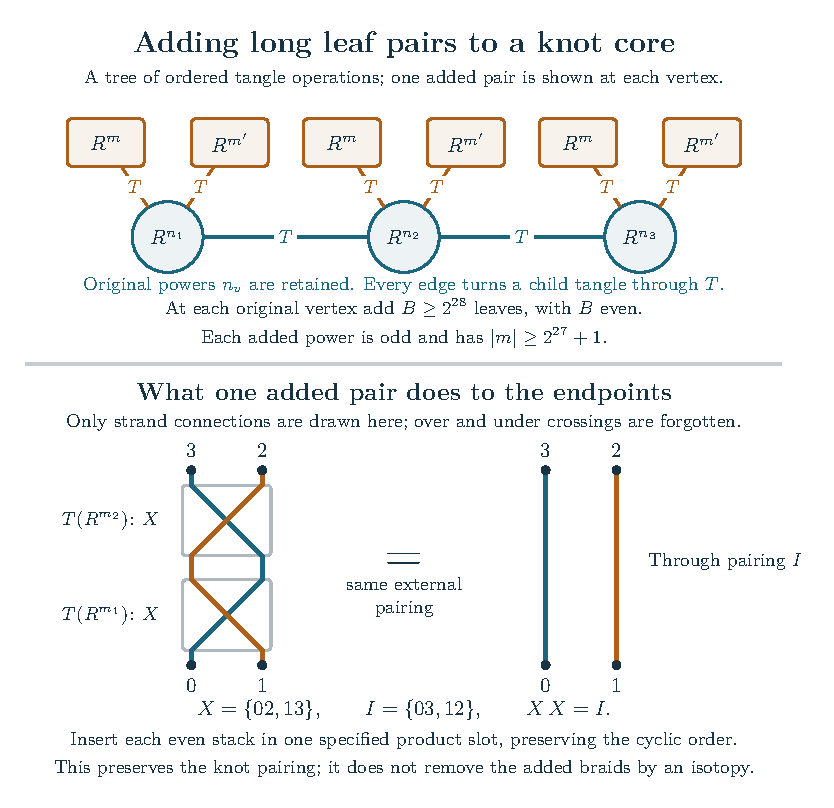
\includegraphics[width=.94\linewidth,keepaspectratio]{../book/figures/directed-tree-volume.pdf}
\caption{An even stack of added odd terminal tangles preserves the core's endpoint pairing.}
\end{figure}

The upper drawing is a tree of tangle operations, not a knot projection.
Only one added pair is drawn at each original vertex. The construction
inserts \(B/2\) consecutive pairs in one specified product slot, retaining
the original cyclic order; \(B\ge2^{28}\) is even. Each added leaf has odd
\(|m|\ge2^{27}+1\), and every tree edge applies the physical quarter-turn
\(T\). The lower drawing forgets crossings and shows the literal endpoint
pairings: two diagonal pairings compose to the through pairing.
It does not claim that the new braids can be removed by an isotopy.

\section{A star beyond both previous quantitative tests}\label{dk:sec-9}

Consider an ordered star rooted at its central vertex, of odd degree
\(d=30{,}000{,}001\). Set its power to 2 and every terminal power to the fixed
odd integer \(2^{60}+1\). Choose \(c_v=k_0/2\) on every leaf.

The knot pairing can be checked in the original terminal-root syntax,
even though the finite contraction is evaluated from the center. Label
the boundary points lower left, lower right, upper right, upper left
by \(0,1,2,3\). The even and odd braid pairings are respectively

\begin{equation}\label{dk:eq-54a}
I=\{03,12\},\qquad X=\{02,13\};\qquad
 T(I)=H=\{01,23\},\quad T(X)=X.
\end{equation}

At a terminal root there are \(d-1\) other leaves. Their turned odd
braids have pairing \(X\); their ordered product has pairing \(I\)
because \(d-1\) is even. The central power \(2\) preserves it. Its
actual quarter-turn has pairing \(H\), and stacking the root's odd
braid against \(H\) still gives \(H\), with no internal closed arc.
Cylindrical closure joins \(03\) and \(12\), so it closes \(H\)
into one component. All intermediate products before that last stack
are two through-strand braids. There is no hidden internal component.

The criterion can be verified by rational enclosures without expanding this large
tree. All leaves have the same data. The center has approximately

\begin{equation}\label{dk:eq-54}
\beta_o=1.219\,10^{-7},\qquad
 \eta_o=2.713\,10^{-7},\qquad
       \frac{\beta_o}{\eta_o/2}<0.9.
\end{equation}

Every leaf has a much smaller ratio. The root does not satisfy the
nonroot patch inequality for any \(c>0\), because \(\beta_o>k_0\chi\).
Nevertheless its exact final trace satisfies \eqref{dk:eq-8}. Thus that outgoing
patch must not be charged to a root that sends no message.

Moreover

\begin{equation}\label{dk:eq-55}
\sum_v\frac{d_v}{d_v^2+n_v^2}
       >\frac{30,000,001}{30,000,001^2+4}>2^{-25},
\end{equation}

and its maximum is far above \(2^{-120}\). The example therefore lies beyond
both published quantitative alternatives. Its size and all its powers
are fixed; it is not an N-growing family. The constant sizes are coarse,
and no optimality assertion is intended.

Here are rational enclosures proving the inequalities rather than
inferring them from those decimal values. Put

\begin{equation}\label{dk:eq-56}
\pi_- =3,\quad \pi_+=22/7,\quad c=k_0/2,\quad
 \chi_-=r_0^2/2-r_0^4/24,\quad
 \delta_- =\frac{c\chi_-}{4(1+c)}.
\end{equation}

At the central vertex use the conservative height
\(y_* =\delta_-/2\). It is at most each branch of \eqref{dk:eq-6}. For example,
with

\begin{equation}\label{dk:eq-57}
D_- =\frac d{2\pi_+},\quad D_+=\frac{d+1}{2\pi_-},\quad
 A_- =\frac{dc}{\pi_+^2},\quad
 C_+=d+\frac{\pi_-^{-2}}{4A_-},
\end{equation}

the three non-strip comparisons are

\begin{equation}\label{dk:eq-58}
y_*<\frac{t_0D_-}{4C_+},\qquad
 y_*<\frac{dc}{8(1+t_0D_+)},\qquad y_*^2<\frac c8.
\end{equation}

The strip comparison follows from \(\delta\ge\delta_-\).
Every quantity in \eqref{dk:eq-56}--\eqref{dk:eq-58} is rational. Direct cross-multiplication
also gives

\begin{equation}\label{dk:eq-59}
\frac{2[420\pi_+d/(361(d^2+4))]}
             {t_0D_-y_*/2}<\frac9{10},
 \qquad
 2\frac{420\pi_+d}{361(d^2+4)}
 <\min\left\{\frac{dc}{2},\ A_-r_0^2,
                          \frac{D_-r_0^2}{8}\right\}.
\end{equation}

These compare the upper bound for twice the first-charge drop with
all four lower bounds for \(\eta_o\). The charge cutoff is greater
than two.

For a leaf with \(n=2^{60}+1\), take
\(y_*=t_0k_0/(2n)\). The same direct rational comparisons, using
\(D_-=n/(2\pi_+)\), \(D_+=(n+1)/(2\pi_-)\),
\(A_-=2k_0/\pi_+^2\), and
\(C_+=16+[n/(2\pi_-)]^2/(4A_-)\), put this height below each
branch of \eqref{dk:eq-6}. They give a lower bound greater than \(2^{-49}\)
for every entry of \eqref{dk:eq-7}, while \(\beta_v<2^{-117}\).
The outgoing patch follows from
\(\beta_v<(k_0/2)\chi_-\). This proves the leaf inequalities.

\section{Reproducing the finite arithmetic and pairings}\label{dk:sec-10}

From the repository root run:

\begin{verbatim}
python3 experiments/audit_actual_all_circle_directed_volume.py
\end{verbatim}

The \href{https://github.com/sashakolpakov/murakamis_dream/blob/main/experiments/audit_actual_all_circle_directed_volume.py}{script}
writes \href{https://github.com/sashakolpakov/murakamis_dream/blob/main/experiments/actual_all_circle_directed_volume_results.json}{its results}.
An optional --output selects a different JSON file. It uses exact rational
arithmetic for the constant inequalities, the all-degree corollaries and
the star enclosures. It also constructs the literal four-endpoint
pairings and checks the composition and closure identities used above.

Those are finite checks, not numerical evidence for the asymptotic
theorem. The proof of the full invariant estimates is the conditional
kernel and trace induction in sections~\ref{dk:sec-2}--\ref{dk:sec-7}. The earlier
\href{https://github.com/sashakolpakov/murakamis_dream/blob/main/experiments/audit_all_circle_local_message_recursion.py}{exact tree-message reproduction}
independently compares canonical quotient contractions with root-grid and
complete first-normal traces; the present argument retains those same
finite identities.

\backmatter
\bibliographystyle{plain}
\bibliography{references}
\end{document}
